\section{Experiments}
\label{sec:experiment}

In this section we analyze the performance of the CGD algorithms derived in Section \ref{sec:fitting} on the specific problem of non-rigid face alignment in-the-wild. 

Results for five experiments are reported. The first experiment compares the fitting accuracy and convergence properties of all algorithms on the test set of the popular Labeled Faces in-the-Wild (LFPW) \cite{Belhumeur2011} database. The second experiment quantifies the importance of the two terms in the Bayesian project-out cost function in relation to the fitting accuracy obtained by Project-Out algorithms. In the third experiment, we study the effect that varying the value of the parameters $\alpha$ and $\beta$ has on the performance of Asymmetric algorithms. The forth experiment explores the effect of optimizing the cost functions using reduced subsets of the total number of pixels and quantifies the impact that this has on the accuracy and computational efficiency of CGD algorithms. Finally, in the fifth and last experiment we report the performance of the most accurate CGD algorithms on the test set of the Helen \cite{Le2012} database and on the entire Annotated Faces in-the-Wild (AFW) \cite{Zhu2012} database.

In all experiments, we use a single AAM, trained using the $\sim800$ and $\sim2000$ training images of the LFPW and Helen databases. Similar to \cite{Tzimiropoulos2014}, we use a modified version of the \emph{Dense} Scale Invariant Feature Transform (DSIFT) \cite{Lowe1999, Dalal2005} to define the appearance representation of the previous AAM. In particular, we describe each pixel with a reduced SIFT descriptor of length $8$ using the public implementation provided by the authors of \cite{Vedaldi2008vlfeat}. All algorithms are implemented in a coarse to fine manner using a Gaussian pyramid with $2$ levels (face images are normalized to a \emph{face size}\footnote{We use the definition of face size given in \cite{Zhu2012} i.e. computed as the mean of the height and width of the bounding box containing the face.} of roughly $150$ pixels at the top level). In all experiments, we optimized over $7$ shape parameters ($4$ similarity transform and $3$ non-rigid shape parameters) at the first pyramid level and over $16$ shape parameters ($4$ similarity transform and $12$ non-rigid shape parameters) at the second one. The dimensionality of the appearance models is kept to represent $75\%$ of the total variance in both levels. This results in $225$ and $280$ appearance parameters at the first and second pyramid levels respectively. The previous choices were determined by testing on a small hold out set of the training data. 

In all experiments, algorithms are initialized by perturbing the similarity transforms that perfectly align the model's mean shape (a frontal pose and neutral expression looking shape) with the ground truth shape of each image. These transforms are perturbed by adding uniformly distributed random noise to their scale, rotation and translation parameters. Exemplar initializations obtained by this procedure for different amounts of noise are shown in Figure \ref{fig:ini}.

Unless stated otherwise:
\begin{inparaenum}[\itshape i\upshape)] 
\item algorithms are initialized with $5\%$ uniform noise;
\item results for Project-Out algorithms are obtained using the Bayesian Project-Out (BPO) cost function defined by Equation \ref{eq:prob_po}; and
\item results for Asymmetric algorithms are reported for the special case of symmetric composition i.e. $\alpha=\beta=0.5$ in Equation \ref{eq:ssd_ac}.
\end{inparaenum}

Landmark annotations for all databases are provided by the iBug group\footnote{\url{http://ibug.doc.ic.ac.uk/resources/300-W/}} and accuracy is reported using the normalized point-to-point error measure proposed in \cite{Zhu2012} over the 49 interior points of the iBug annotation scheme.

Finally, in order to encourage open research and facilitate future comparisons with the results presented in this section, we make the implementation of all CGD algorithms publicly available as part of the Menpo Project \cite{Menpo2014}.


\subsection{Comparison on LFPW}

In this experiment, we report the fitting accuracy and convergence properties of all CGD algorithms studied in this paper. Results are reported on the $\sim220$ test images of the LFPW database. In order to keep the information easily readable and interpretable, we group algorithms by cost function i.e. (SSD or BPO), and optimization method (i.e. Gauss-Newton, Newton or Wiberg).

Results for this experiment are reported in Figures \ref{fig:ssd_gn_5}, \ref{fig:ssd_n_5}, \ref{fig:ssd_w_5}, \ref{fig:bpo_gn_5}, \ref{fig:bpo_n_5} and \ref{fig:bpo_w_5}. These figures have all the same structure and are composed of four figures and a table. Figures \ref{fig:ced_ssd_gn_5}, \ref{fig:ced_ssd_n_5}, \ref{fig:ced_ssd_w_5}, \ref{fig:ced_bpo_gn_5}, \ref{fig:ced_bpo_n_5} and \ref{fig:ced_bpo_w_5} report the Cumulative Error Distribution (CED), i.e the proportion of images vs normalized point-to-point error. Tables \ref{tab:stats_ssd_gn_5}, \ref{tab:stats_ssd_n_5}, \ref{tab:stats_ssd_w_5}, \ref{tab:stats_bpo_gn_5}, \ref{tab:stats_bpo_n_5}, and \ref{tab:stats_bpo_w_5} summarize and complete the information on the previous CEDs by stating the proportion of images fitted with a normalized point-to-point error smaller than $0.02$, $0.03$ and $0.04$; and by stating the mean, std and median of the final normalized point-to-point error. The aim of the previous figures and tables is to help us compare the final fitting accuracy obtained by each algorithm. On the other hand, Figures \ref{fig:mean_error_vs_iters_ssd_gn_5}, \ref{fig:mean_error_vs_iters_ssd_n_5}, \ref{fig:mean_error_vs_iters_ssd_w_5}, \ref{fig:mean_error_vs_iters_bpo_gn_5}, \ref{fig:mean_error_vs_iters_bpo_n_5} and \ref{fig:mean_error_vs_iters_bpo_w_5} report the mean normalized point-to-point error at each iteration while Figures \ref{fig:mean_cost_vs_iters1_ssd_gn_5}, \ref{fig:mean_cost_vs_iters2_ssd_gn_5}, \ref{fig:mean_cost_vs_iters1_ssd_n_5}, \ref{fig:mean_cost_vs_iters2_ssd_n_5}, \ref{fig:mean_cost_vs_iters1_ssd_w_5}, \ref{fig:mean_cost_vs_iters2_ssd_w_5}, \ref{fig:mean_cost_vs_iters1_bpo_gn_5}, \ref{fig:mean_cost_vs_iters2_bpo_gn_5}, \ref{fig:mean_cost_vs_iters1_bpo_n_5}, \ref{fig:mean_cost_vs_iters2_bpo_n_5} and \ref{fig:mean_cost_vs_iters1_bpo_w_5}, \ref{fig:mean_cost_vs_iters2_bpo_w_5} report the mean normalized cost at each iteration\footnote{The Figures are produced by dividing the value of the cost function at each iteration by its initial value and averaging for all images.}. The aim of the previous figures is to help us compare the convergence properties of every algorithm.


\subsubsection{SSD Gauss-Newton algorithms}

Results for \emph{SSD Gauss-Newton} algorithms are reported in Figure \ref{fig:ssd_gn_5}. We can observe that \emph{Inverse}, \emph{Asymmetric} and \emph{Bidirectional} algorithms obtain a similar performance and significantly outperform \emph{Forward} algorithms in terms of fitting accuracy, Figure \ref{fig:ced_ssd_gn_5} and Table \ref{tab:stats_ssd_gn_5}. In absolute terms, \emph{Bidirectional} algorithms slightly outperform \emph{Inverse} and \emph{Asymmetric} algorithms however this difference in performance was not found to be statistically significant. On the other hand, the difference in performance between the \emph{Simultaneous Schur} and \emph{Alternated} optimizations strategies for each algorithm are minimal and they were found to have no statistical significance.

On the other hand, looking at Figures \ref{fig:mean_error_vs_iters_ssd_gn_5}, \ref{fig:mean_cost_vs_iters1_ssd_gn_5} and \ref{fig:mean_cost_vs_iters2_ssd_gn_5} there seems to be a clear (and obviously expected) correlation between the normalized point-to-point error and the normalized value of the cost function at each iteration. In terms of convergence, it can be seen that \emph{Forward} algorithms converge slower than \emph{Inverse}, \emph{Asymmetric} and \emph{Bidirectional}. \emph{Bidirectional} algorithms converge slightly faster than \emph{Inverse} algorithms and these slightly faster than \emph{Asymmetric} algorithms. In this case, the \emph{Simultaneous Schur} optimization strategy seems to converge slightly faster than the \emph{Alternated} one for all \emph{SSD Gauss-Newton} algorithms.


\subsubsection{SSD Newton algorithms}

Results for \emph{SSD Newton} algorithms are reported on Figure \ref{fig:ssd_n_5}. In this case, we can observe that the fitting performance of all algorithms decreases with respect to their \emph{Gauss-Newton} counterparts \ref{fig:ced_ssd_n_5} and Table \ref{tab:stats_ssd_n_5}. This is most noticeable in the case of \emph{Forward} algorithms for which there is $\sim20\%$ drop in the proportion of images fitted below $0.02$, $0.03$ and $0.04$ with respect to its \emph{Gauss-Newton} equivalents. For these algorithms there is also a significant increase in the mean and median of the normalized point-to-point error. \emph{Asymmetric Newton} algorithms also perform considerably worse, between $5\%$ and $10\%$, than their \emph{Gauss-Newton} versions. This drop in performance is reduced for \emph{Inverse} and \emph{Bidirectional Newton} algorithms for which accuracy is reduced by around $3\%$ with respect their \emph{Gauss-Newton} equivalent. 

Within Newton algorithms, there are clear differences in terms of speed of convergence \ref{fig:mean_error_vs_iters_ssd_n_5}, \ref{fig:mean_cost_vs_iters1_ssd_n_5} and \ref{fig:mean_cost_vs_iters2_ssd_n_5}. Bidirectional algorithms are the fastest to converge followed by Inverse and Asymmetric algorithms, in this order, and lastly Forward algorithms. In this case, the \emph{Simultaneous Schur} optimization strategy seems to converge again slightly faster than the \emph{Alternated} one for all algorithms but \emph{Bidirectional} algorithms, for which the \emph{Alternated} strategy converges slightly faster.

\subsubsection{SSD Wiberg algorithms}

Results for SSD Wiberg algorithms are reported on Figure \ref{fig:ssd_w_5}. Figure \ref{fig:ced_ssd_w_5} and Table \ref{tab:stats_ssd_w_5} and Figures \ref{fig:mean_error_vs_iters_ssd_w_5}, \ref{fig:mean_cost_vs_iters1_ssd_w_5} and \ref{fig:mean_cost_vs_iters2_ssd_w_5} show that these results are (as we would expect) virtually equivalent to those obtained by their \emph{Gauss-Newton} counterparts.

\begin{figure*}[t!]
	\centering
	\begin{subfigure}{0.16\textwidth}
		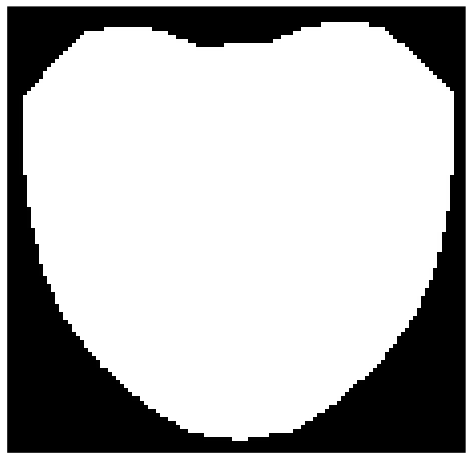
\includegraphics[width=\textwidth]{figures/sampling_100.png}
		\caption{$100\%$}
		\label{fig:sampling_100}
	\end{subfigure}
	\begin{subfigure}{0.16\textwidth}
		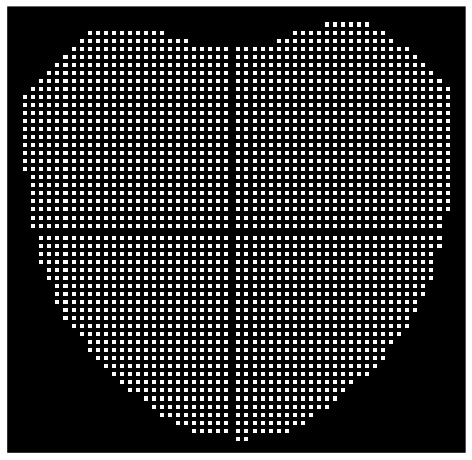
\includegraphics[width=\textwidth]{figures/sampling_50.png}
		\caption{$50\%$}
		\label{fig:sampling_50}
	\end{subfigure}
	\begin{subfigure}{0.16\textwidth}
		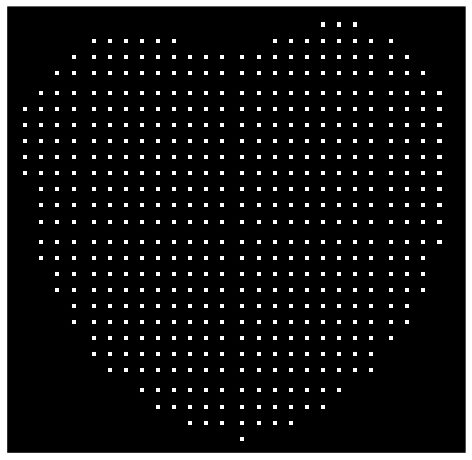
\includegraphics[width=\textwidth]{figures/sampling_25.png}
		\caption{$25\%$}
		\label{fig:sampling_25}
	\end{subfigure}
	\begin{subfigure}{0.16\textwidth}
		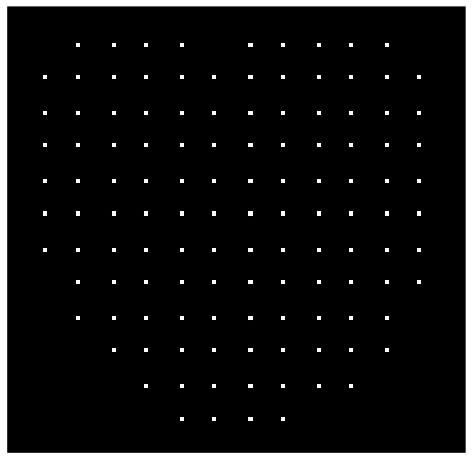
\includegraphics[width=\textwidth]{figures/sampling_12.png}
		\caption{$12\%$}
		\label{fig:ini_12}
	\end{subfigure}
	\caption{Subset of pixels on the reference frame used to optimize the SSD and Project-Out cost functions for different rates of sampling.}
    \label{fig:sampling_masks}
\end{figure*}


\begin{figure*}[p]
	\centering
	\begin{subfigure}{0.48\textwidth}
	    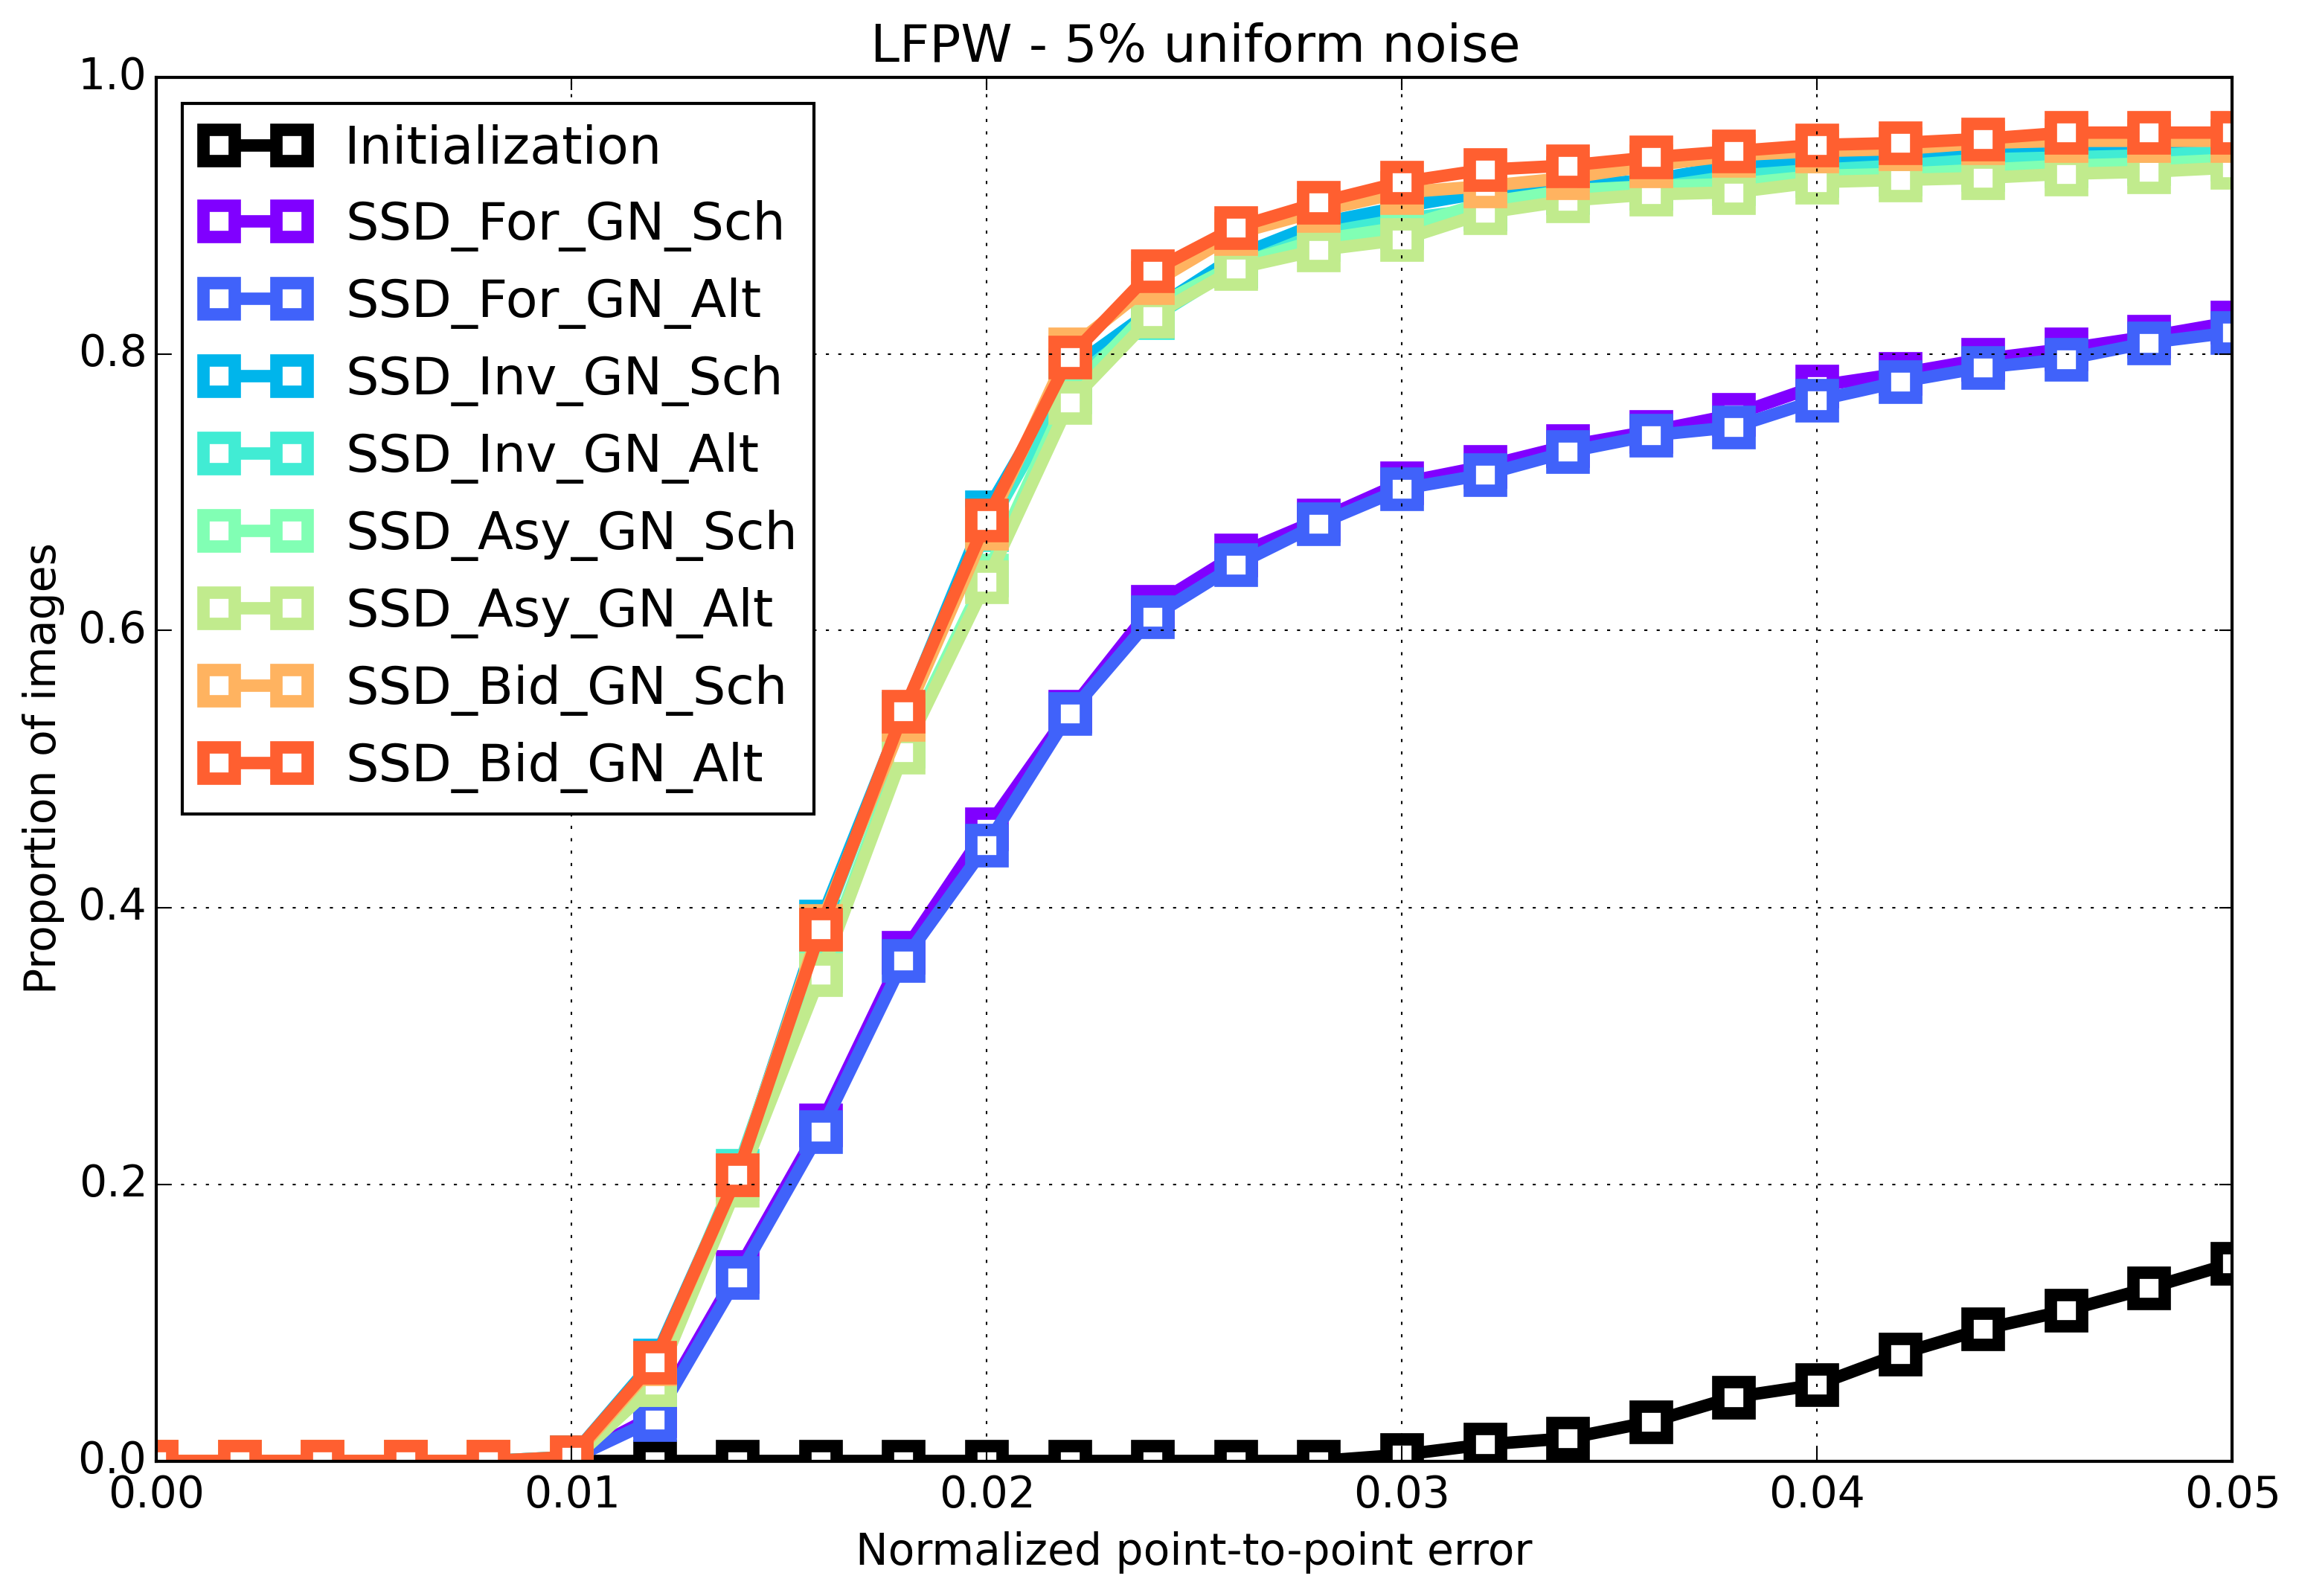
\includegraphics[width=\textwidth]{experiments/algorithms/ssd_gn/ced_ssd_gn_5.png}
	    \caption{Cumulative error distribution on the LFPW test dataset for all SSD Gauss-Newton algorithms initialized with $5\%$ uniform noise.}
	    \label{fig:ced_ssd_gn_5}
	\end{subfigure}
	\hfill
	\begin{subfigure}{0.48\textwidth}
	    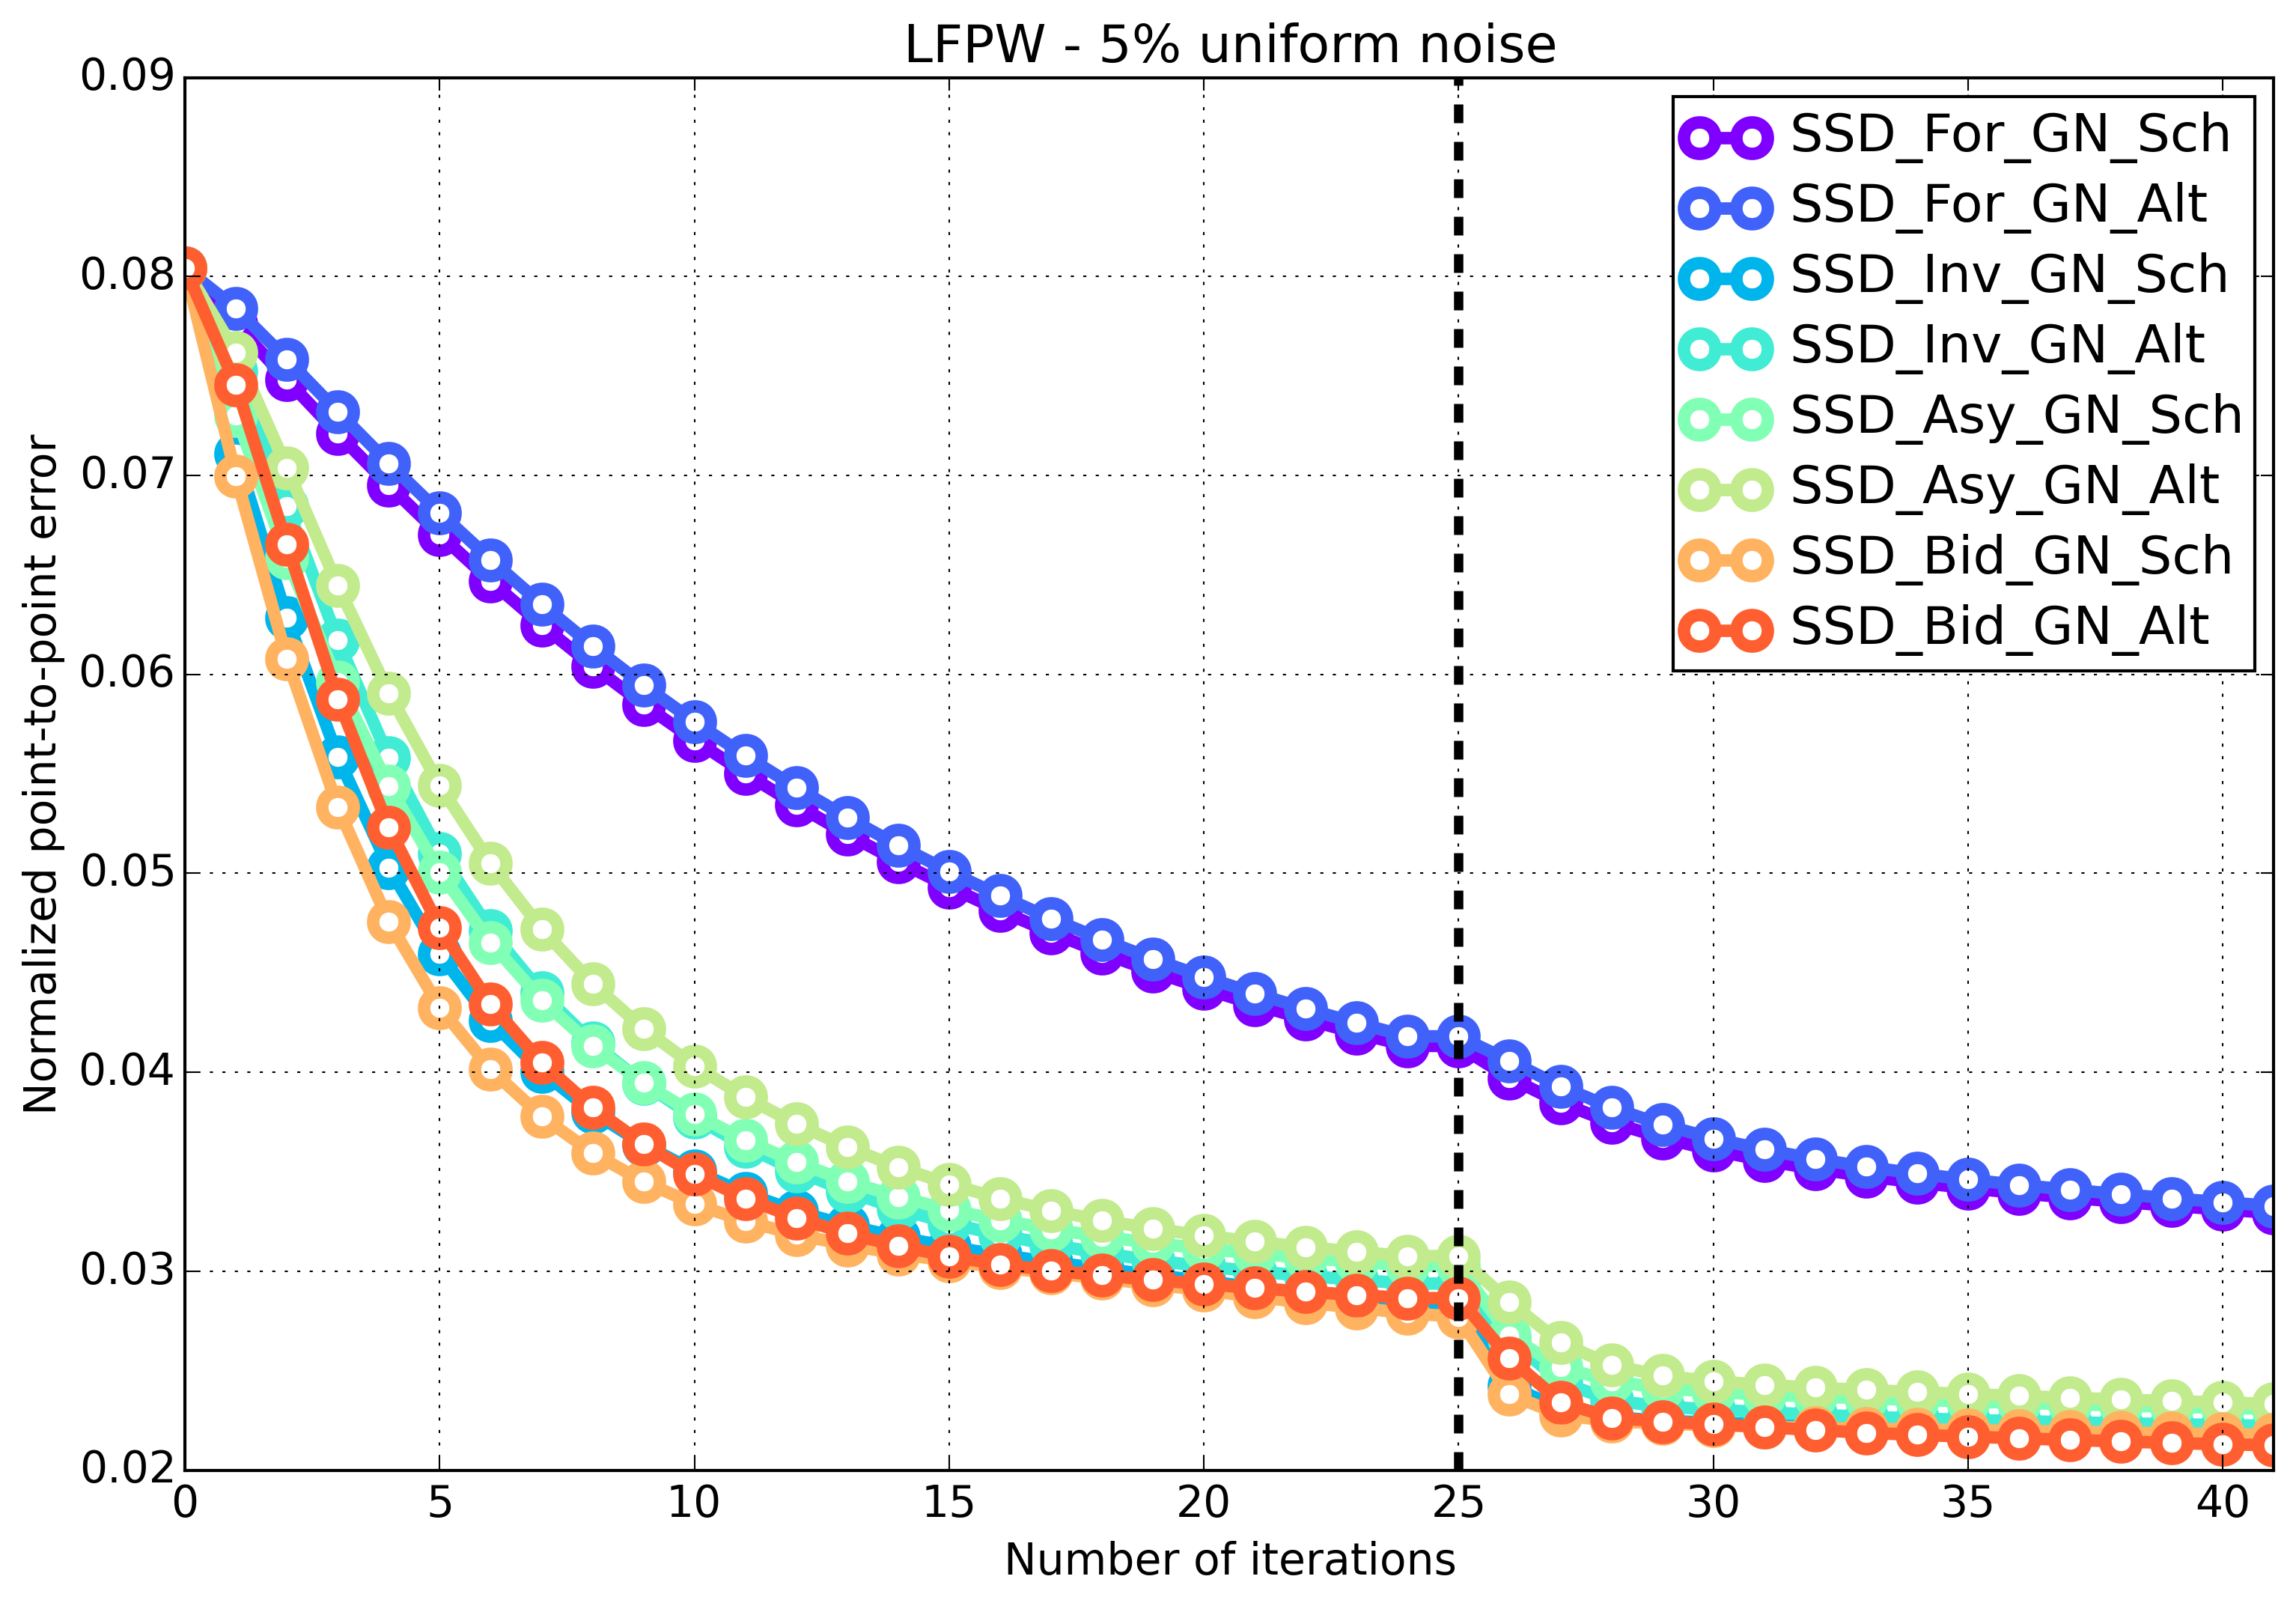
\includegraphics[width=\textwidth]{experiments/algorithms/ssd_gn/mean_error_vs_iters_ssd_gn_5.png}
	    \caption{Mean normalized point-to-point error vs number of iterations on the LFPW test dataset for all SSD Gauss-Newton algorithms initialized with $5\%$ uniform noise.}
	    \label{fig:mean_error_vs_iters_ssd_gn_5}
	\end{subfigure}
	\par\bigskip\bigskip
	\begin{subfigure}{0.48\textwidth}
	    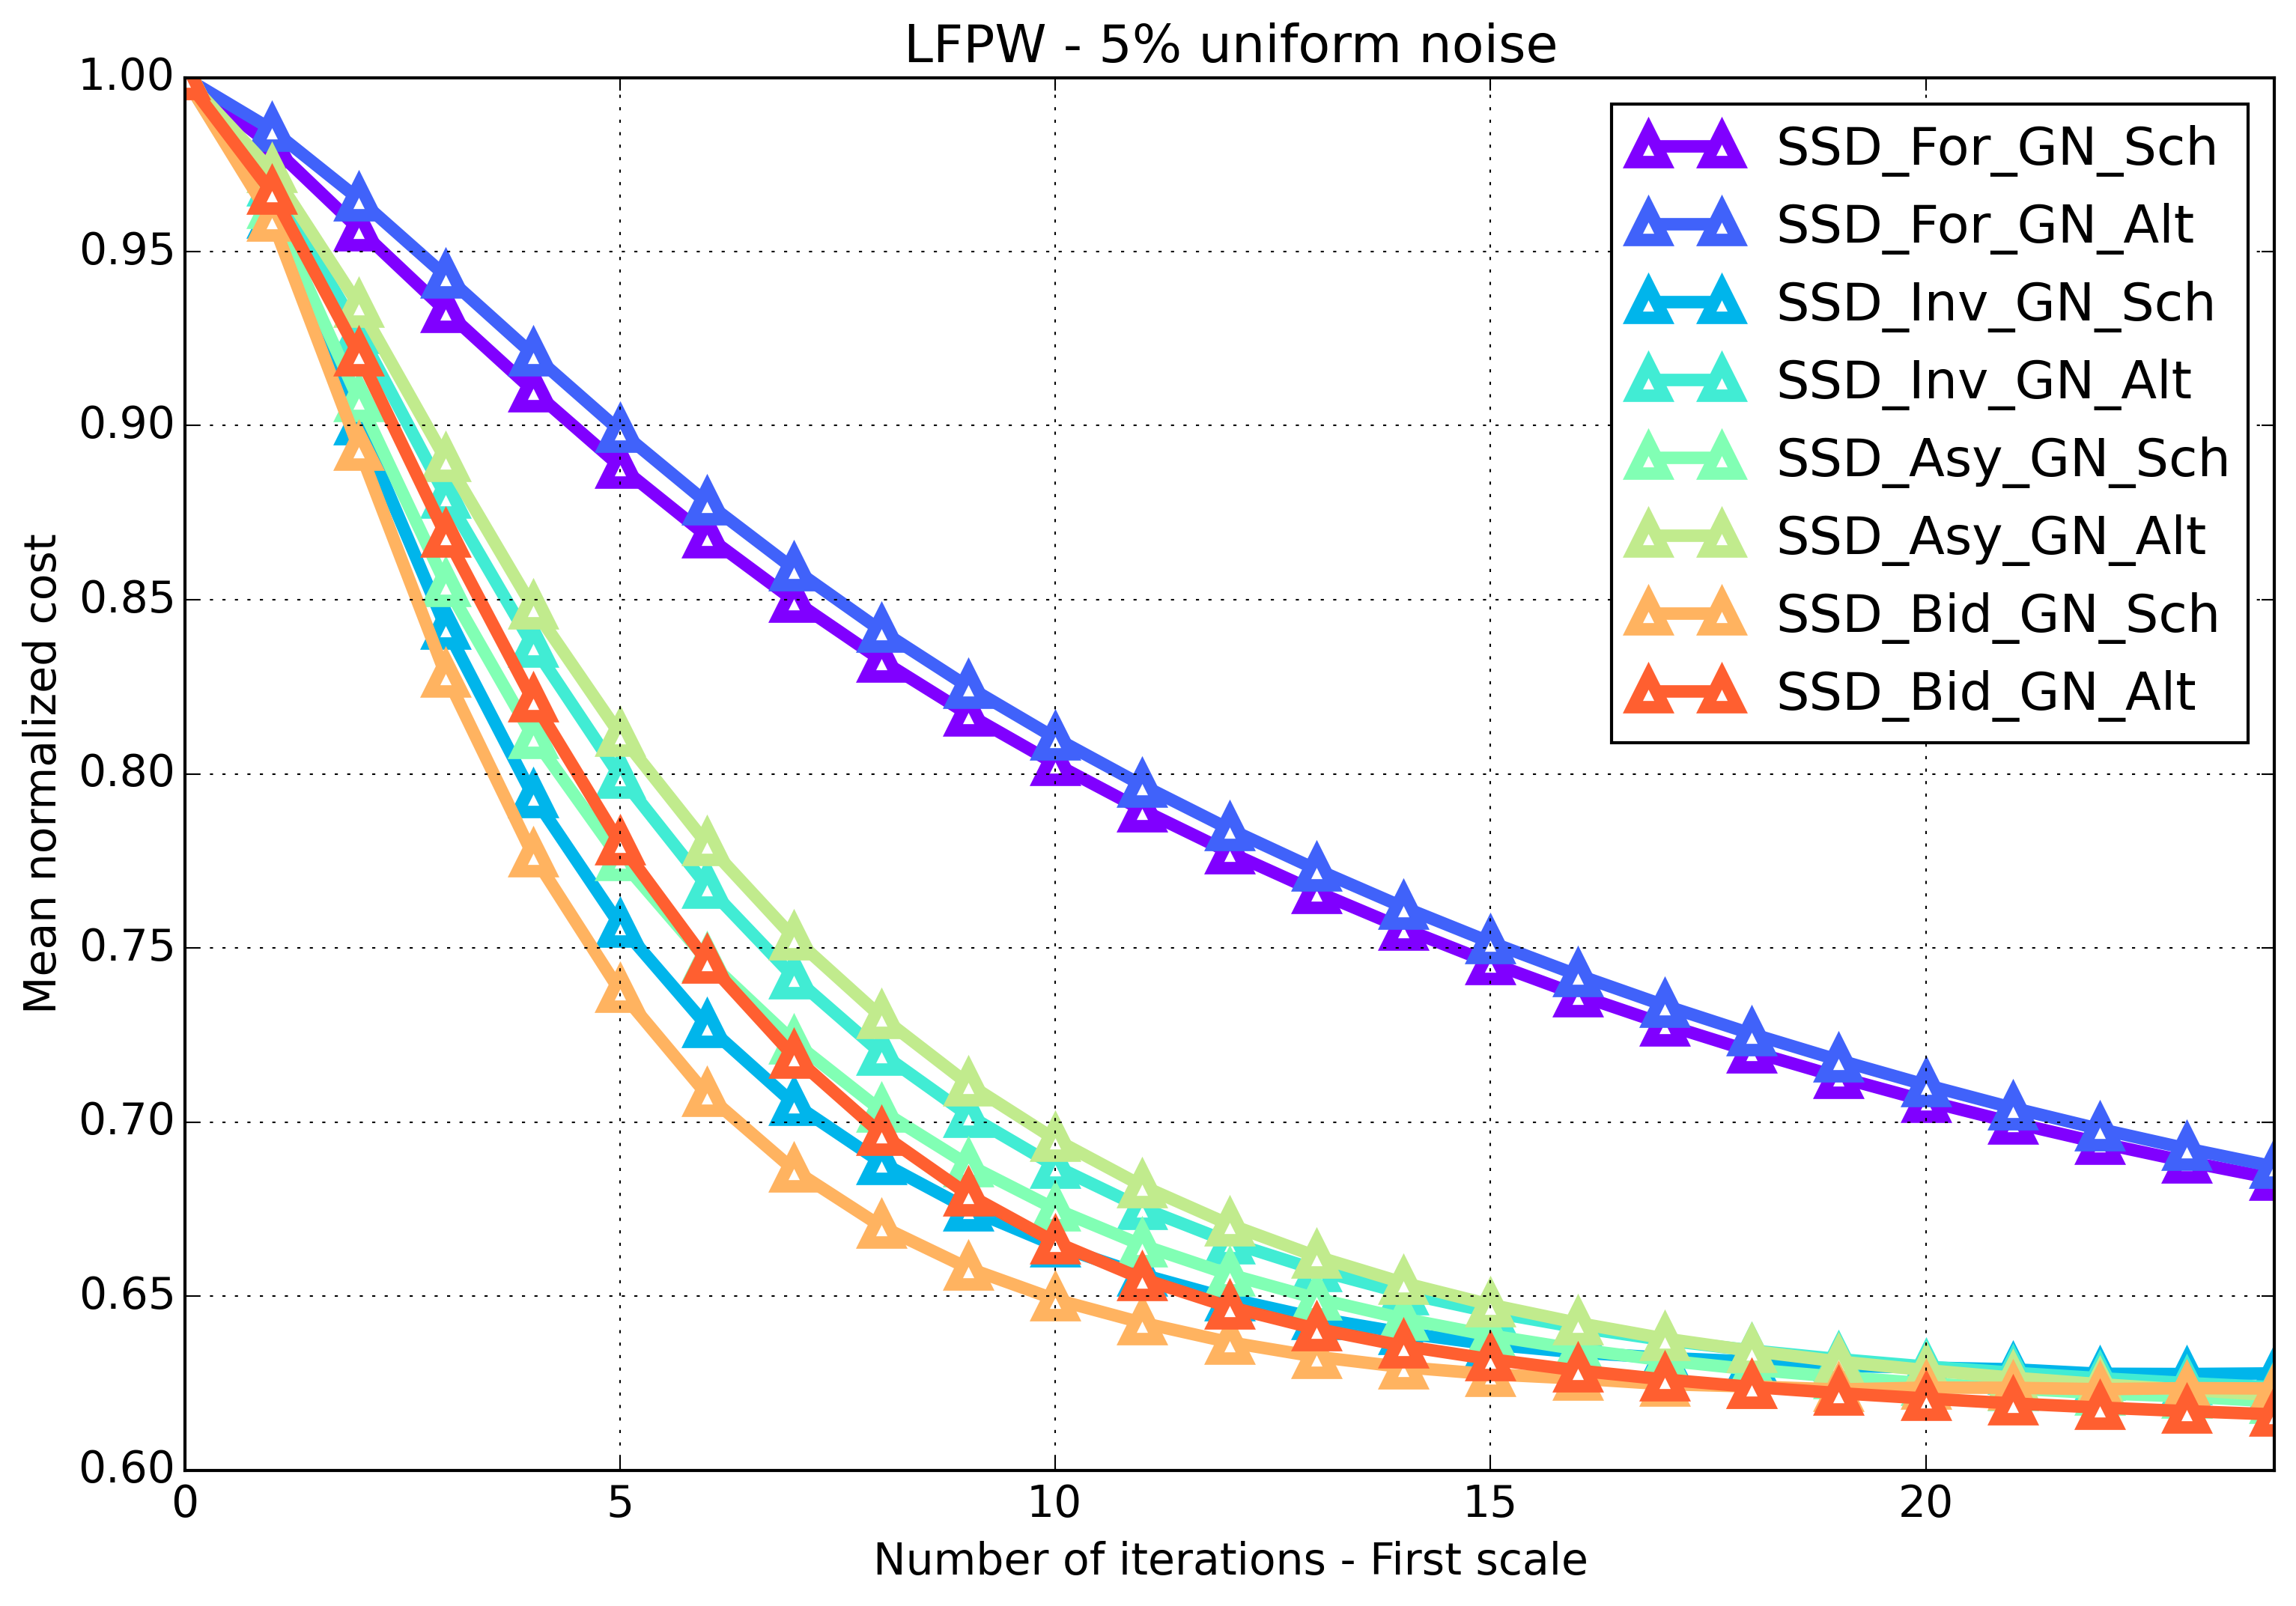
\includegraphics[width=\textwidth]{experiments/algorithms/ssd_gn/mean_cost_vs_iters1_ssd_gn_5.png}
	    \caption{Mean normalized cost vs number of first scale iterations on the LFPW test dataset for all SSD Gauss-Newton algorithms initialized with $5\%$ uniform noise.}
	    \label{fig:mean_cost_vs_iters1_ssd_gn_5}
	\end{subfigure}
	\hfill
	\begin{subfigure}{0.48\textwidth}
	    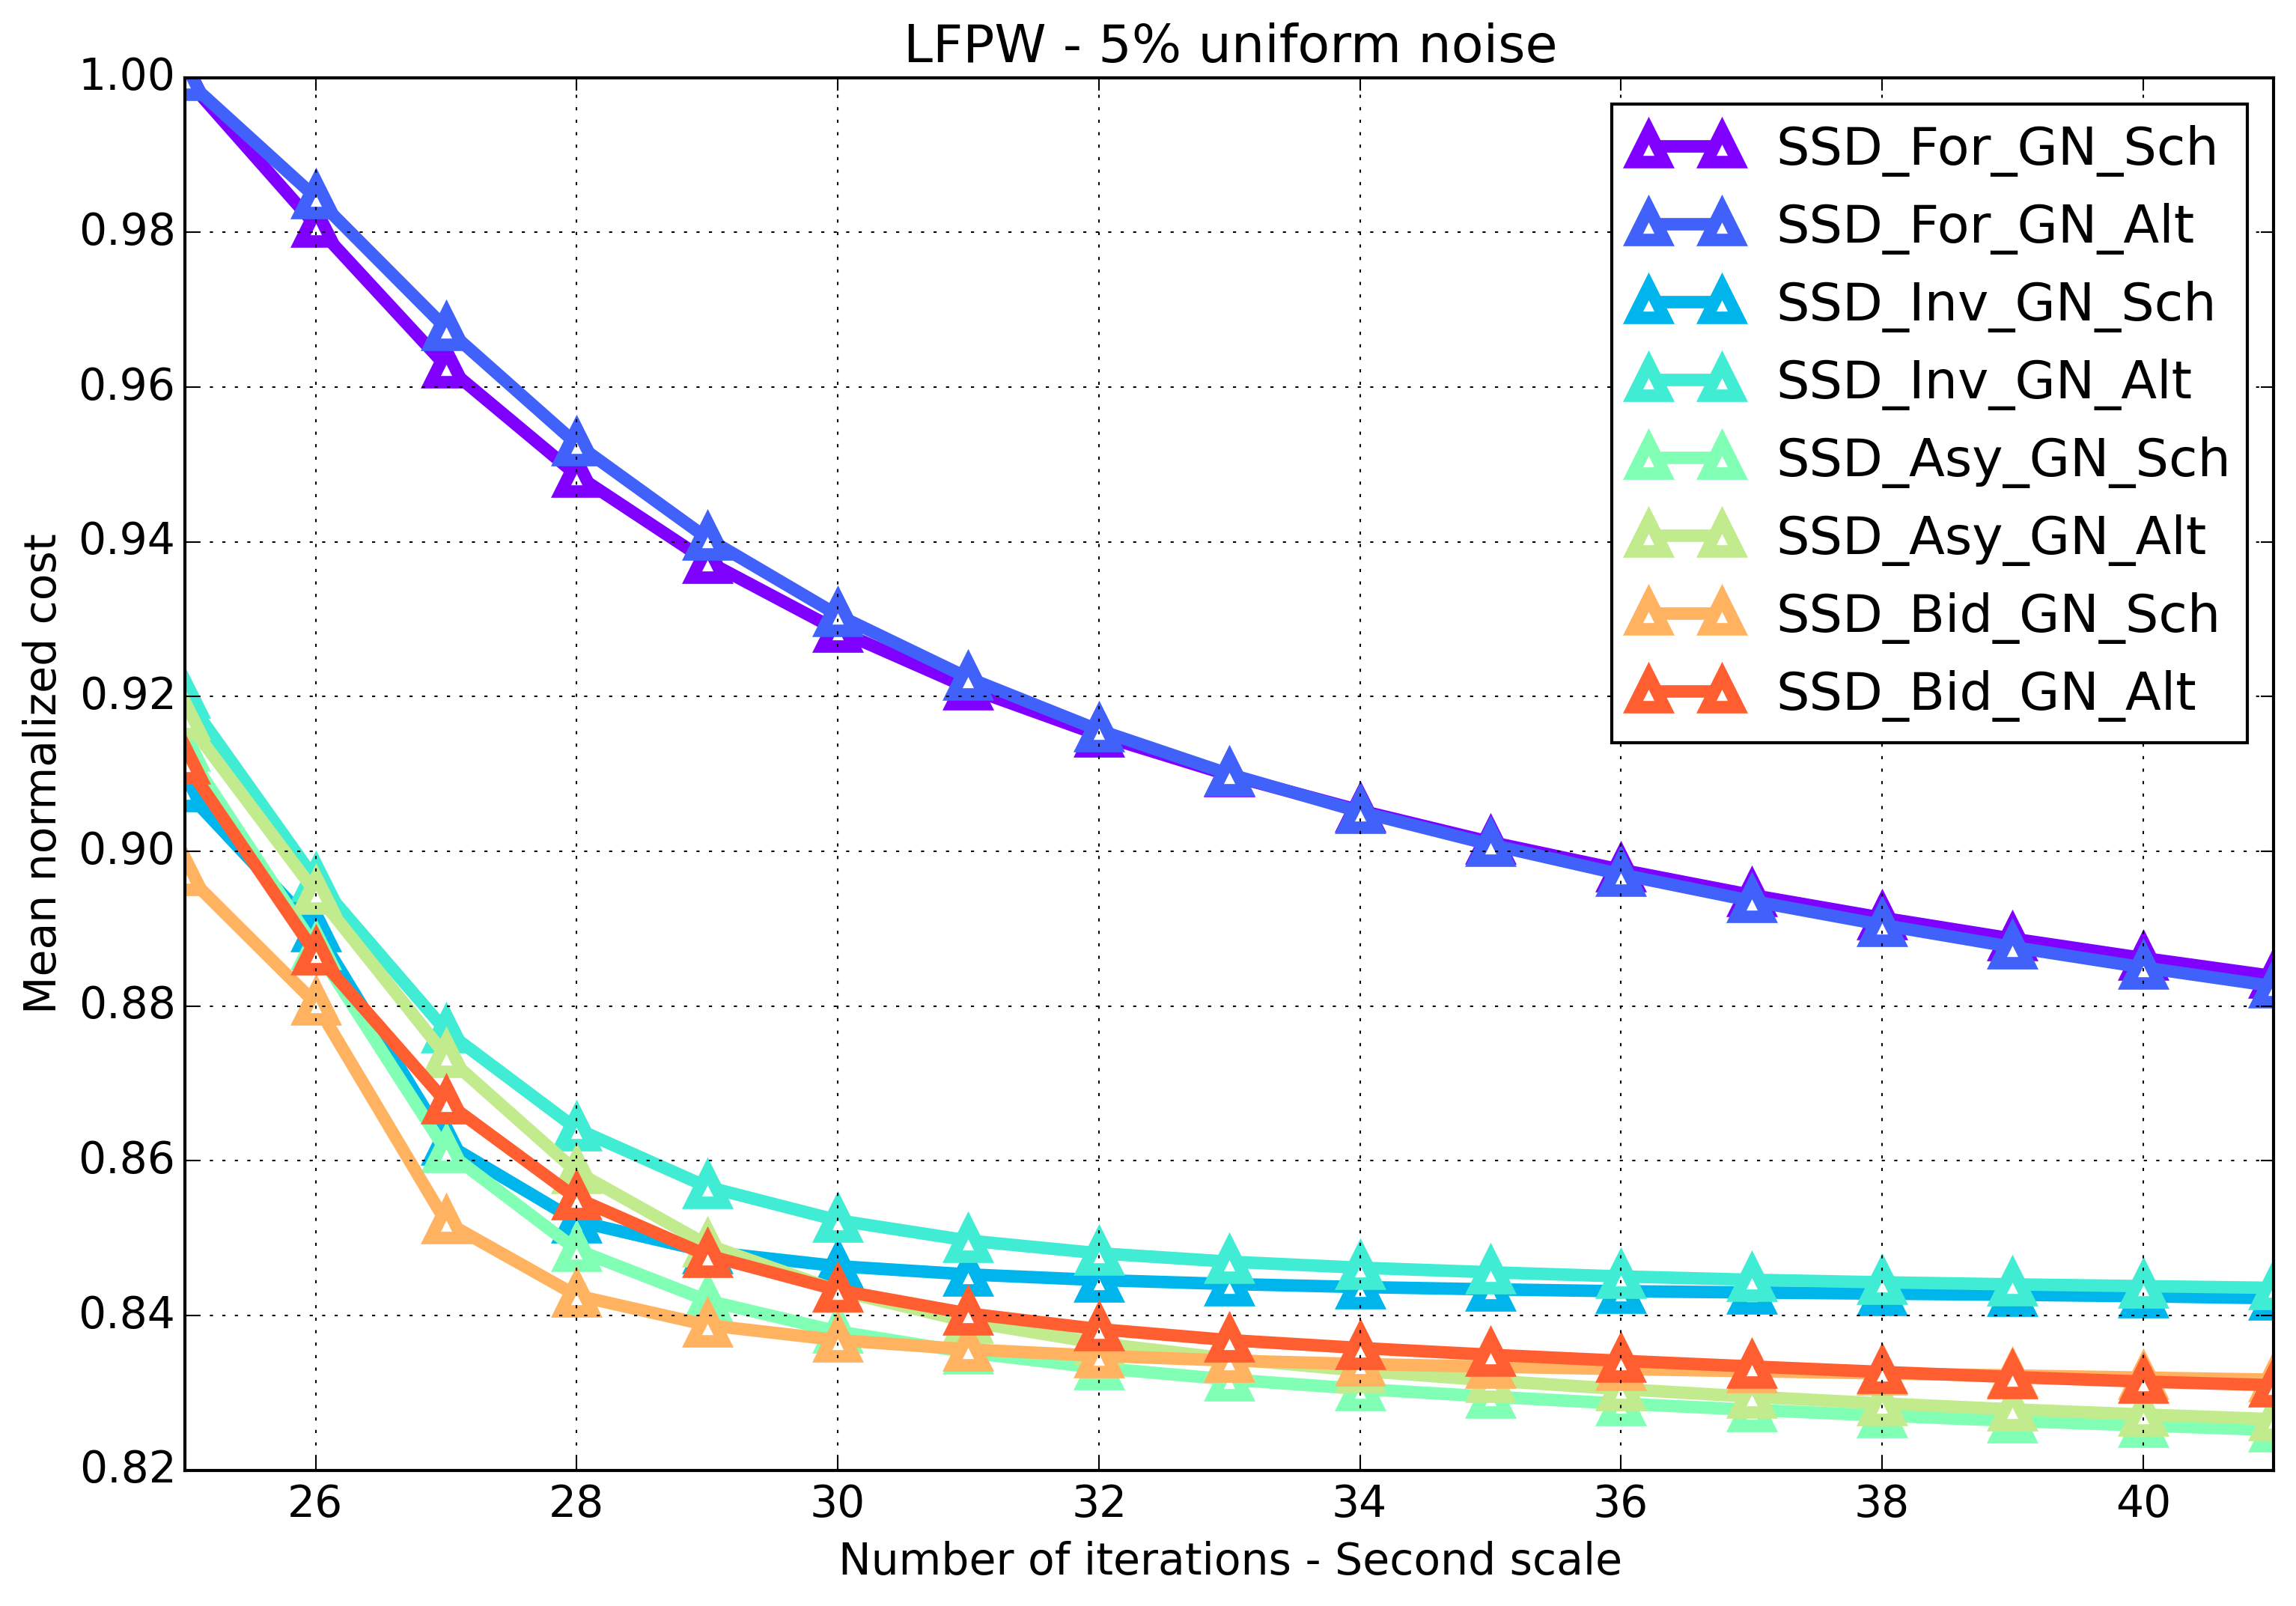
\includegraphics[width=\textwidth]{experiments/algorithms/ssd_gn/mean_cost_vs_iters2_ssd_gn_5.png}
	    \caption{Mean normalized cost vs number of second scale iterations on the LFPW test dataset for all SSD Gauss-Newton algorithms initialized with $5\%$ uniform noise.}
	    \label{fig:mean_cost_vs_iters2_ssd_gn_5}
	\end{subfigure}
	\par\bigskip\bigskip
	\begin{subfigure}{\textwidth}
		\center
		\begin{tabular}{lcccccc}
			\toprule
		    Algorithm & $<0.02$ & $<0.03$ & $<0.04$ & Mean & Sdt & Median 
		    \\
		    \midrule
		    Initialization & 0.000 & 0.004 & 0.055 & 0.080 & 0.028 & 0.078
		    \\
		    SSD\_For\_GN\_Sch & 0.456 & 0.707 & 0.777 & 0.033 & 0.030 & 0.021 
		    \\
		    SSD\_For\_GN\_Alt & 0.445 & 0.702 & 0.766 & 0.033 & 0.030 & 0.021
		    \\
		    SSD\_Inv\_GN\_Sch & 0.686 & 0.906 & 0.939 & 0.022 & \textbf{0.019} & \textbf{0.017}
		    \\
		    SSD\_Inv\_GN\_Alt & 0.673 & 0.897 & 0.933 & 0.022 & 0.020 & \textbf{0.017}
		    \\
		    SSD\_Asy\_GN\_Sch & 0.640 & 0.891 & 0.929 & 0.023 & 0.021 & 0.018
		    \\
		    SSD\_Asy\_GN\_Alt & 0.635 & 0.882 & 0.924 & 0.023 & 0.021 & 0.018
		    \\
		    SSD\_Bid\_GN\_Sch & 0.674 & 0.917 & 0.946 & 0.022 & \textbf{0.019} & \textbf{0.017}
		    \\
		    SSD\_Bid\_GN\_Alt & \textbf{0.680} & \textbf{0.924} & \textbf{0.951} & \textbf{0.021} & \textbf{0.019} & \textbf{0.017} 
		    \\
		    \bottomrule
	  	\end{tabular}
	  	\caption{Table showing the proportion of images fitted with a normalized point-to-point error below $0.02$, $0.03$ and $0.04$ together with the normalized point-to-point error Mean, Std and Median for all SSD Gauss-Newton algorithms initialized with $5\%$ uniform noise.}
	    \label{tab:stats_ssd_gn_5}
	\end{subfigure}
	\caption{Results showing the fitting accuracy and convergence properties of the SSD Gauss-Newton algorithms on the LFPW test dataset initialized with $5\%$ uniform noise.}
	\label{fig:ssd_gn_5}
\end{figure*}


\begin{figure*}[p]
	\centering
	\begin{subfigure}{0.48\textwidth}
	    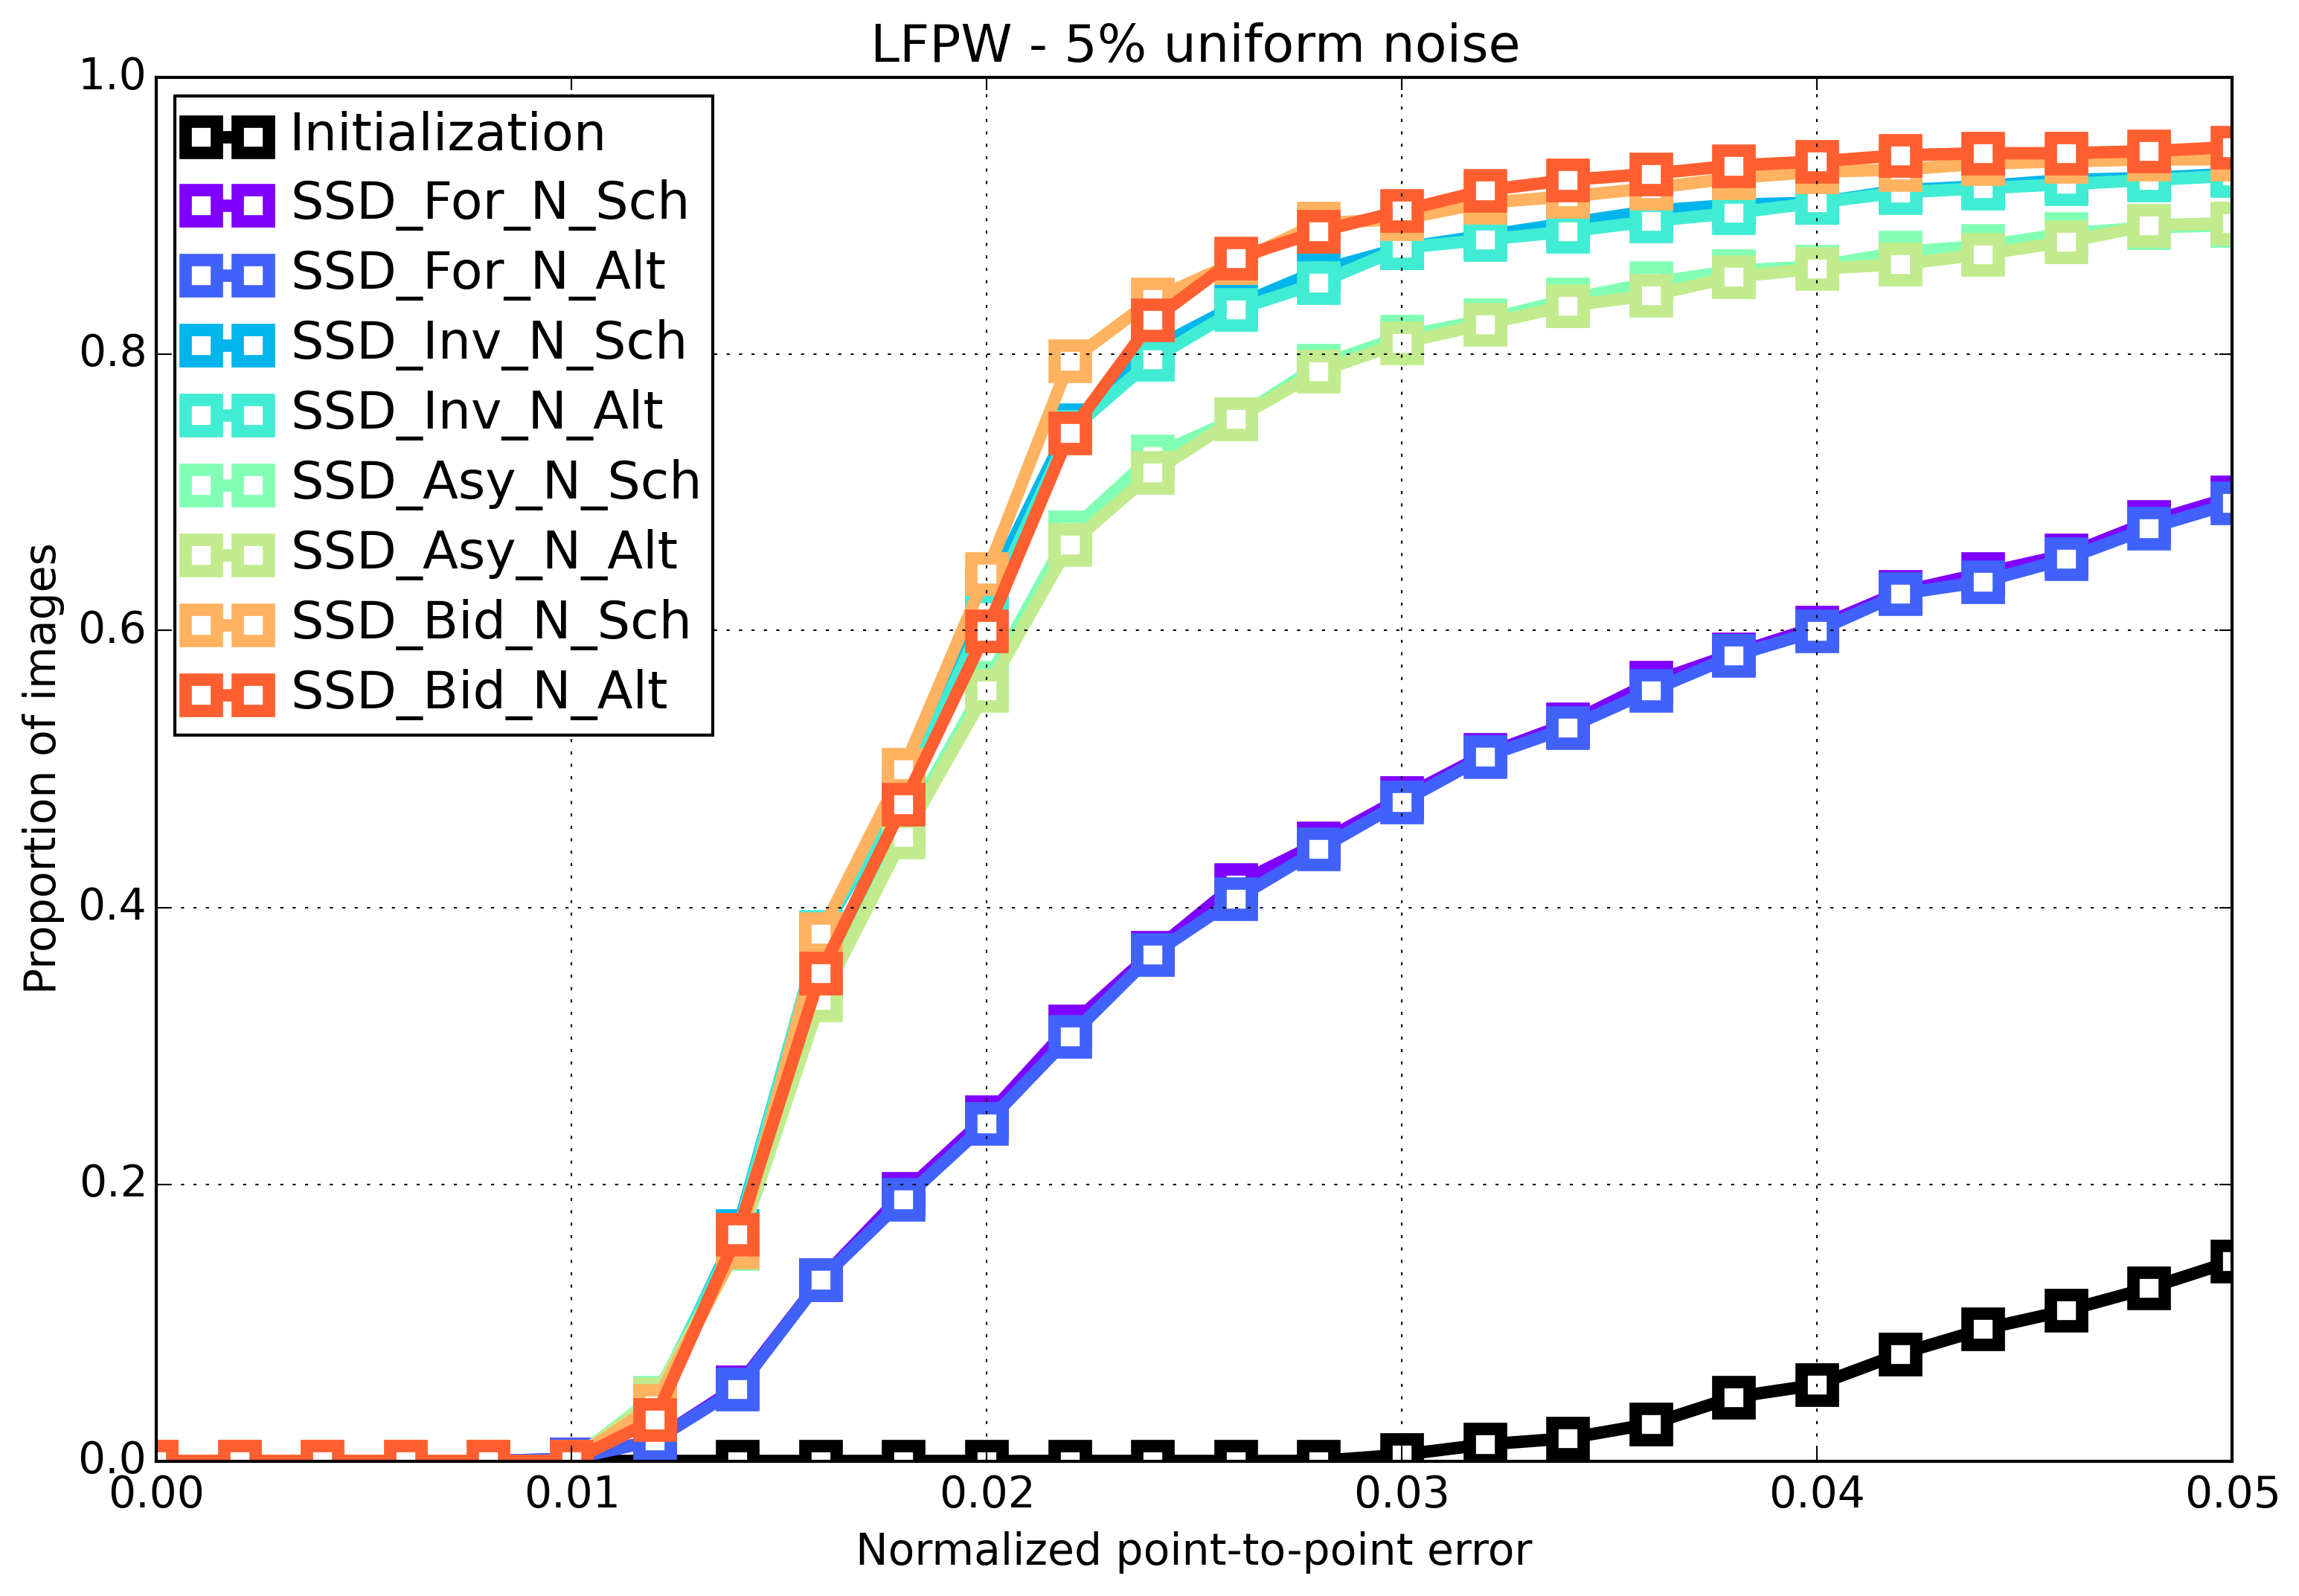
\includegraphics[width=\textwidth]{experiments/algorithms/ssd_n/ced_ssd_n_5.png}
	    \caption{Cumulative error distribution on the LFPW test dataset for all SSD Newton algorithms initialized with $5\%$ uniform noise.}
	    \label{fig:ced_ssd_n_5}
	\end{subfigure}
	\hfill
	\begin{subfigure}{0.48\textwidth}
	    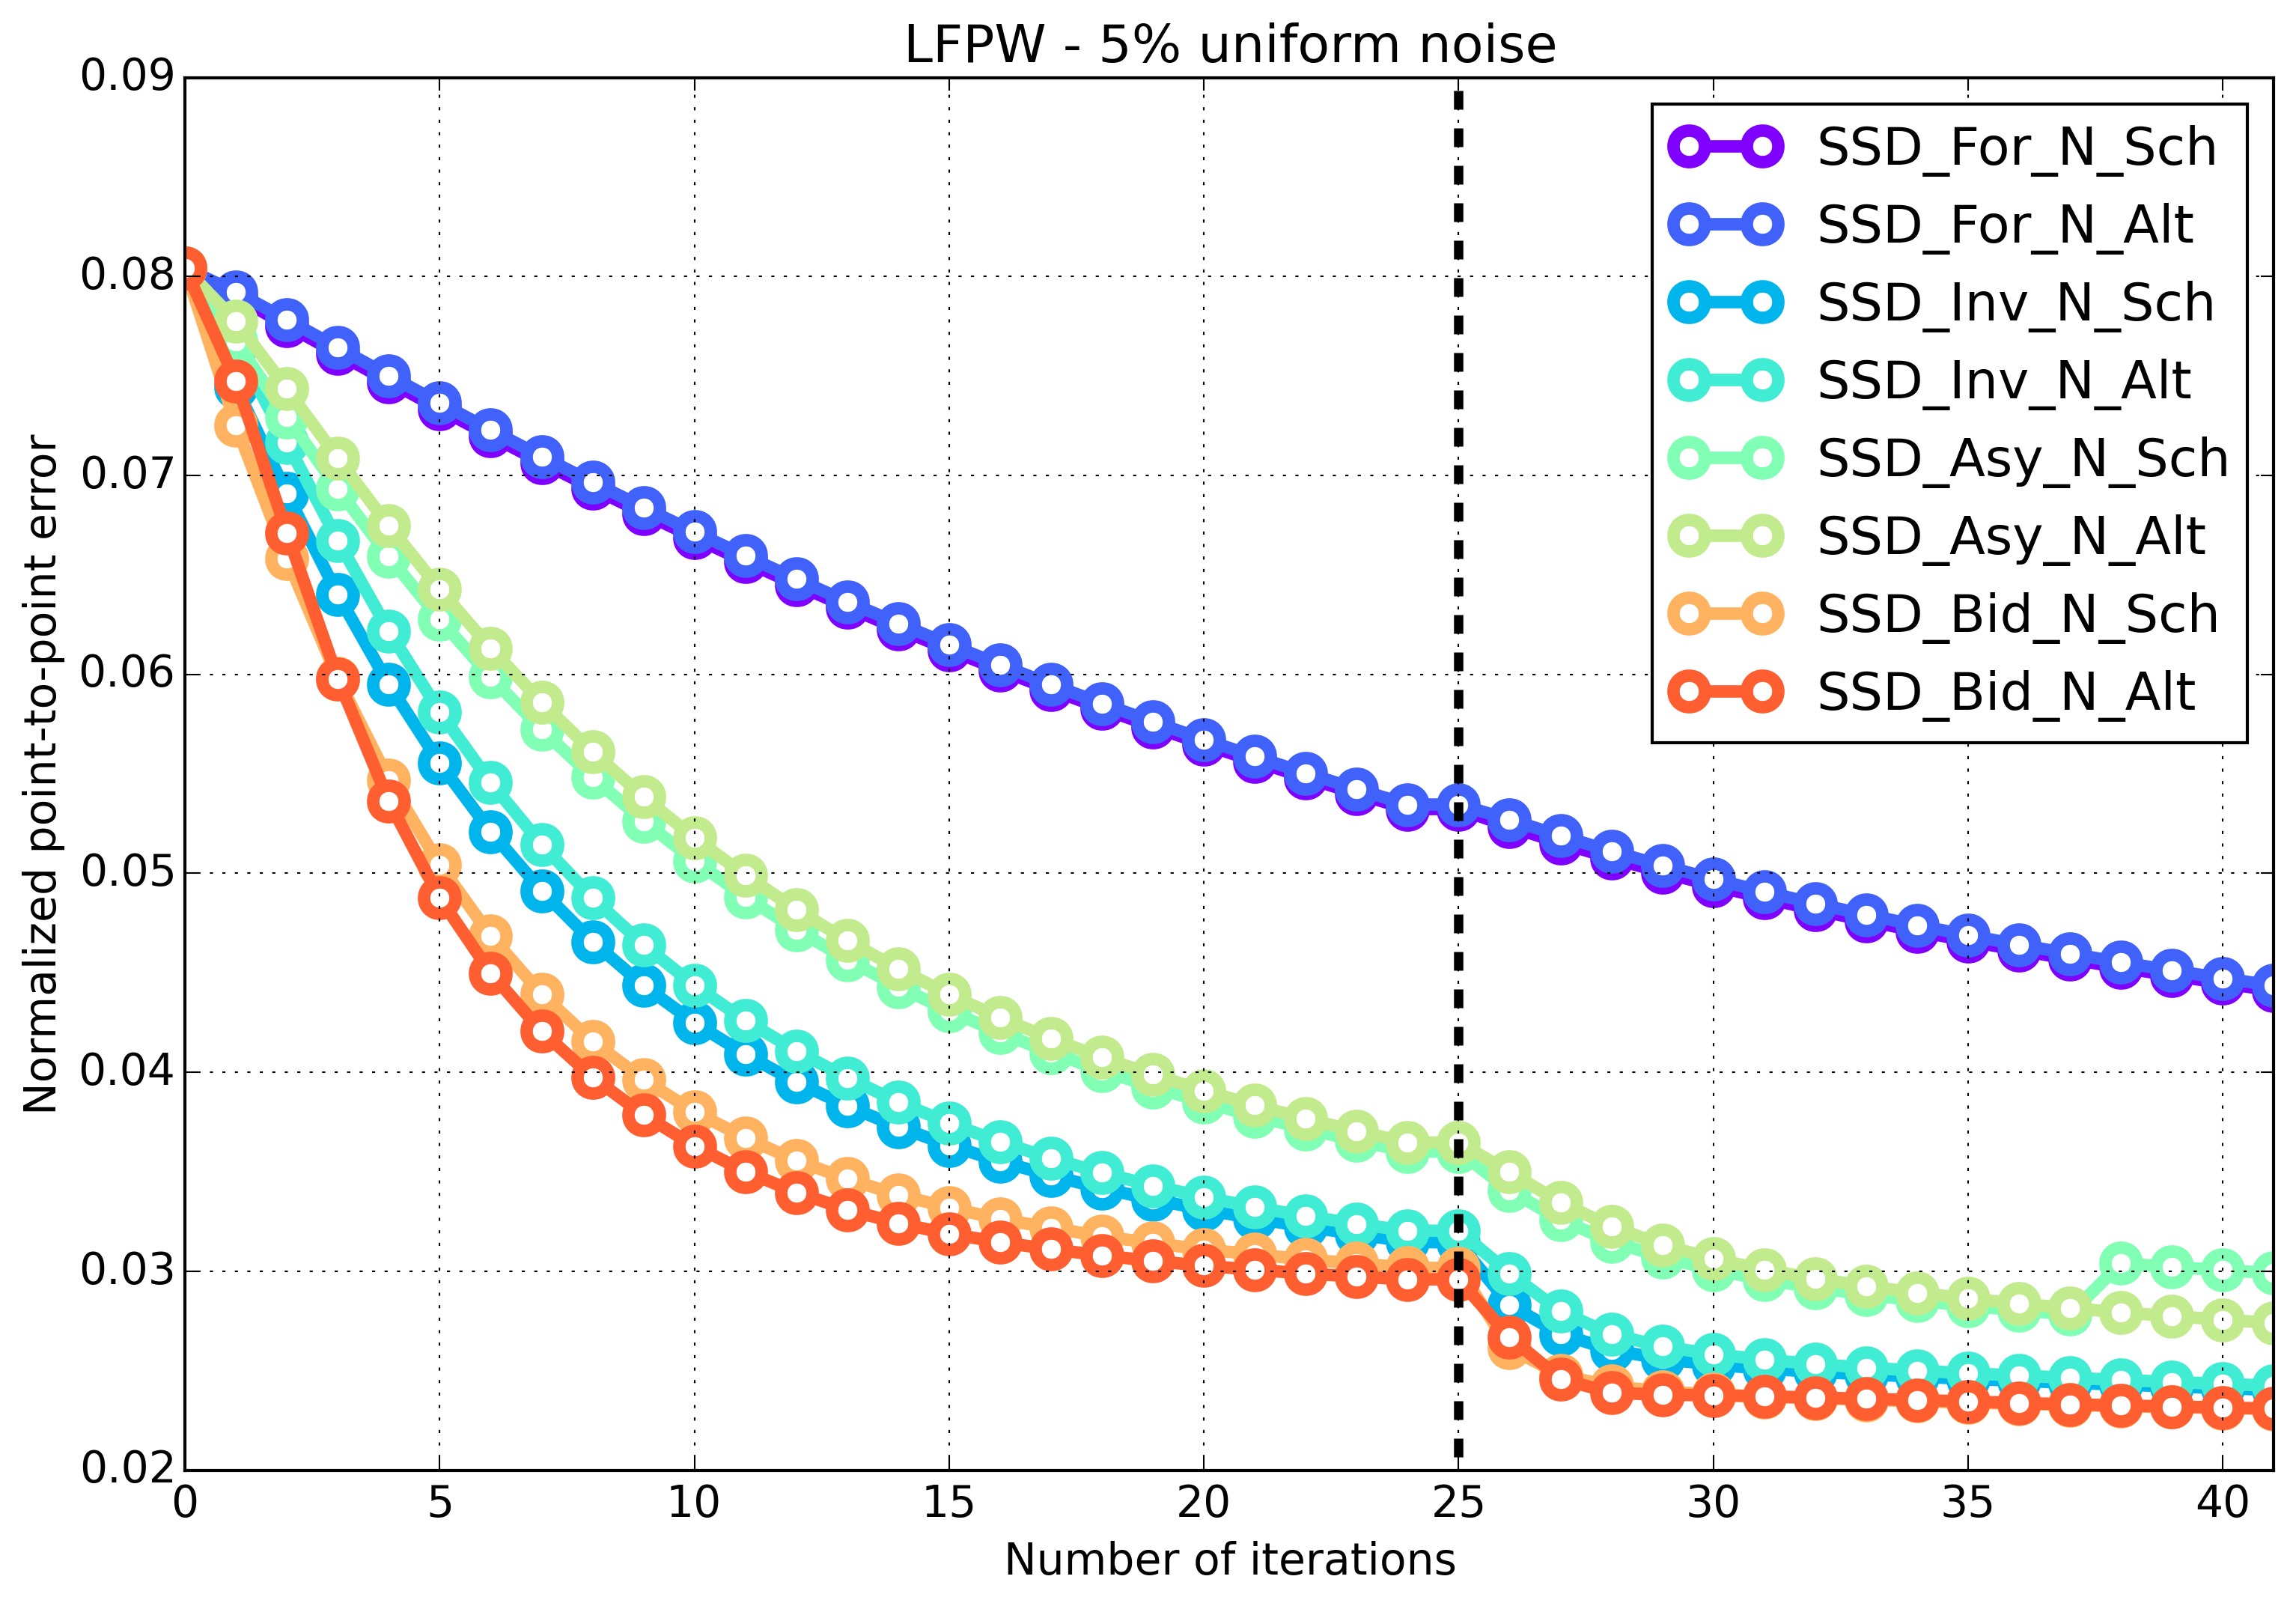
\includegraphics[width=\textwidth]{experiments/algorithms/ssd_n/mean_error_vs_iters_ssd_n_5.png}
	    \caption{Mean normalized point-to-point error vs number of iterations on the LFPW test dataset for all SSD Newton algorithms initialized with $5\%$ uniform noise.}
	    \label{fig:mean_error_vs_iters_ssd_n_5}
	\end{subfigure}
	\par\bigskip\bigskip
	\begin{subfigure}{0.48\textwidth}
	    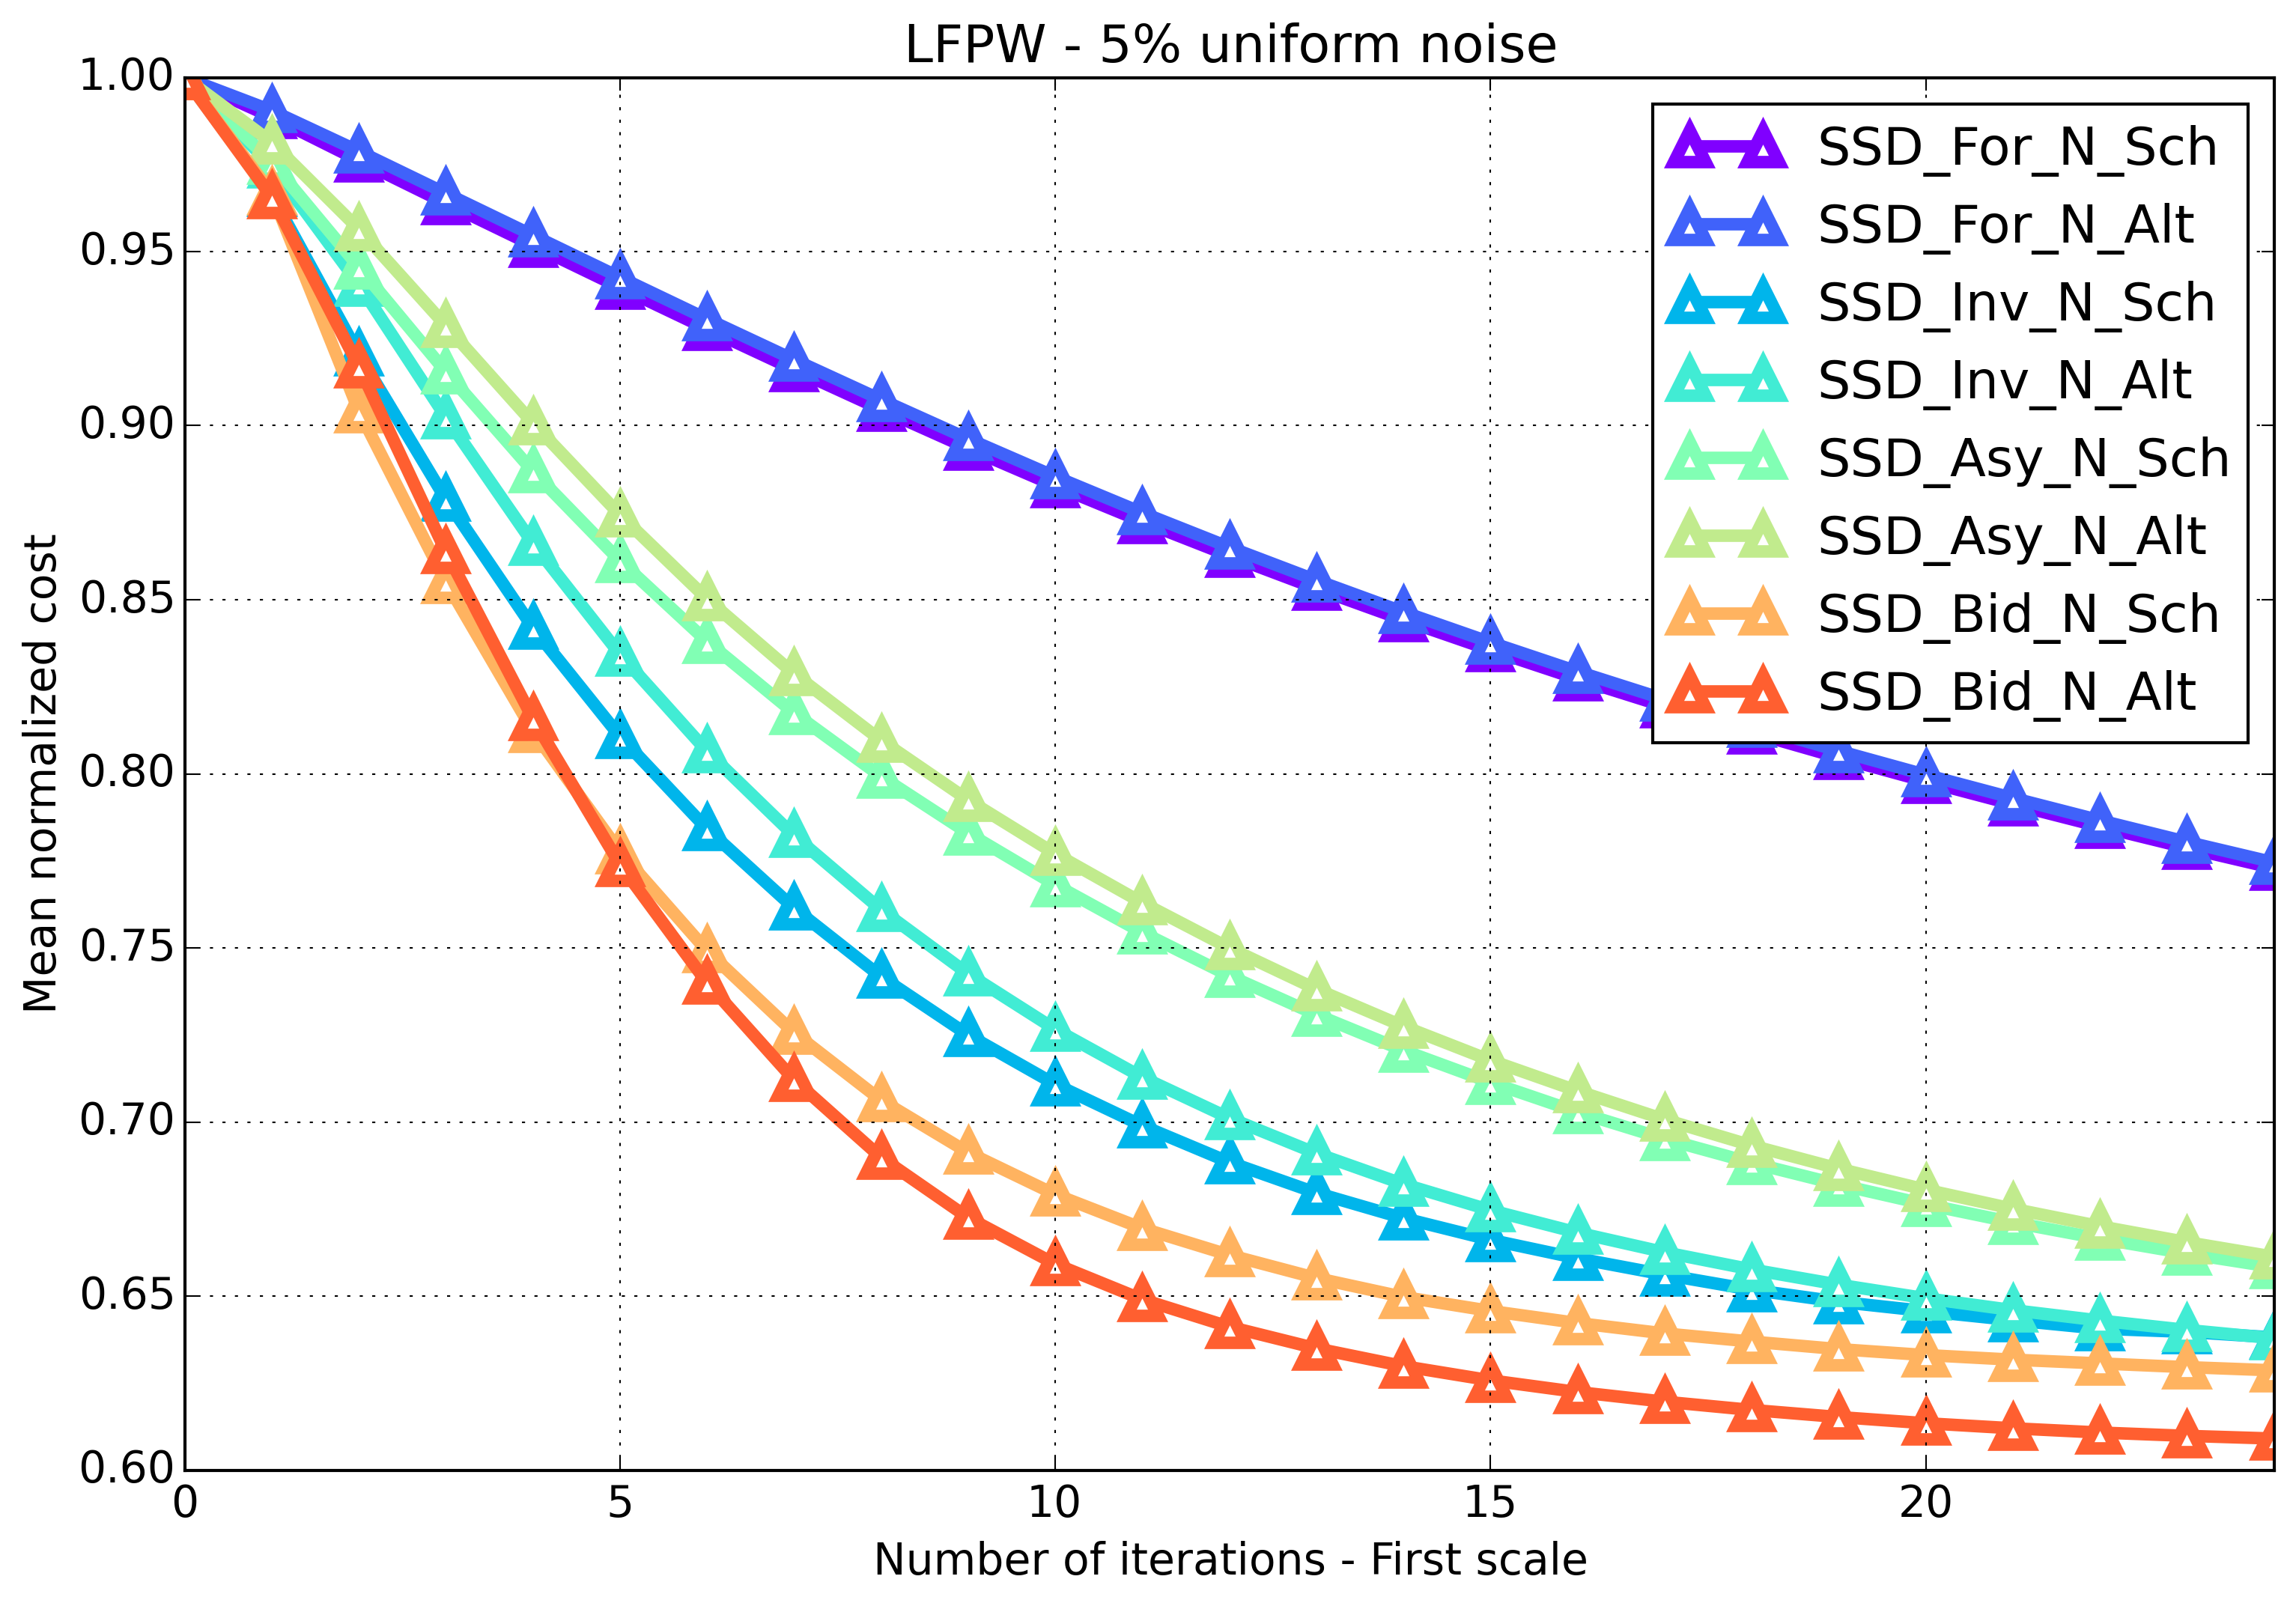
\includegraphics[width=\textwidth]{experiments/algorithms/ssd_n/mean_cost_vs_iters1_ssd_n_5.png}
	    \caption{Mean normalized cost vs number of first scale iterations on the LFPW test dataset for all SSD Newton algorithms initialized with $5\%$ uniform noise.}
	    \label{fig:mean_cost_vs_iters1_ssd_n_5}
	\end{subfigure}
	\hfill
	\begin{subfigure}{0.48\textwidth}
	    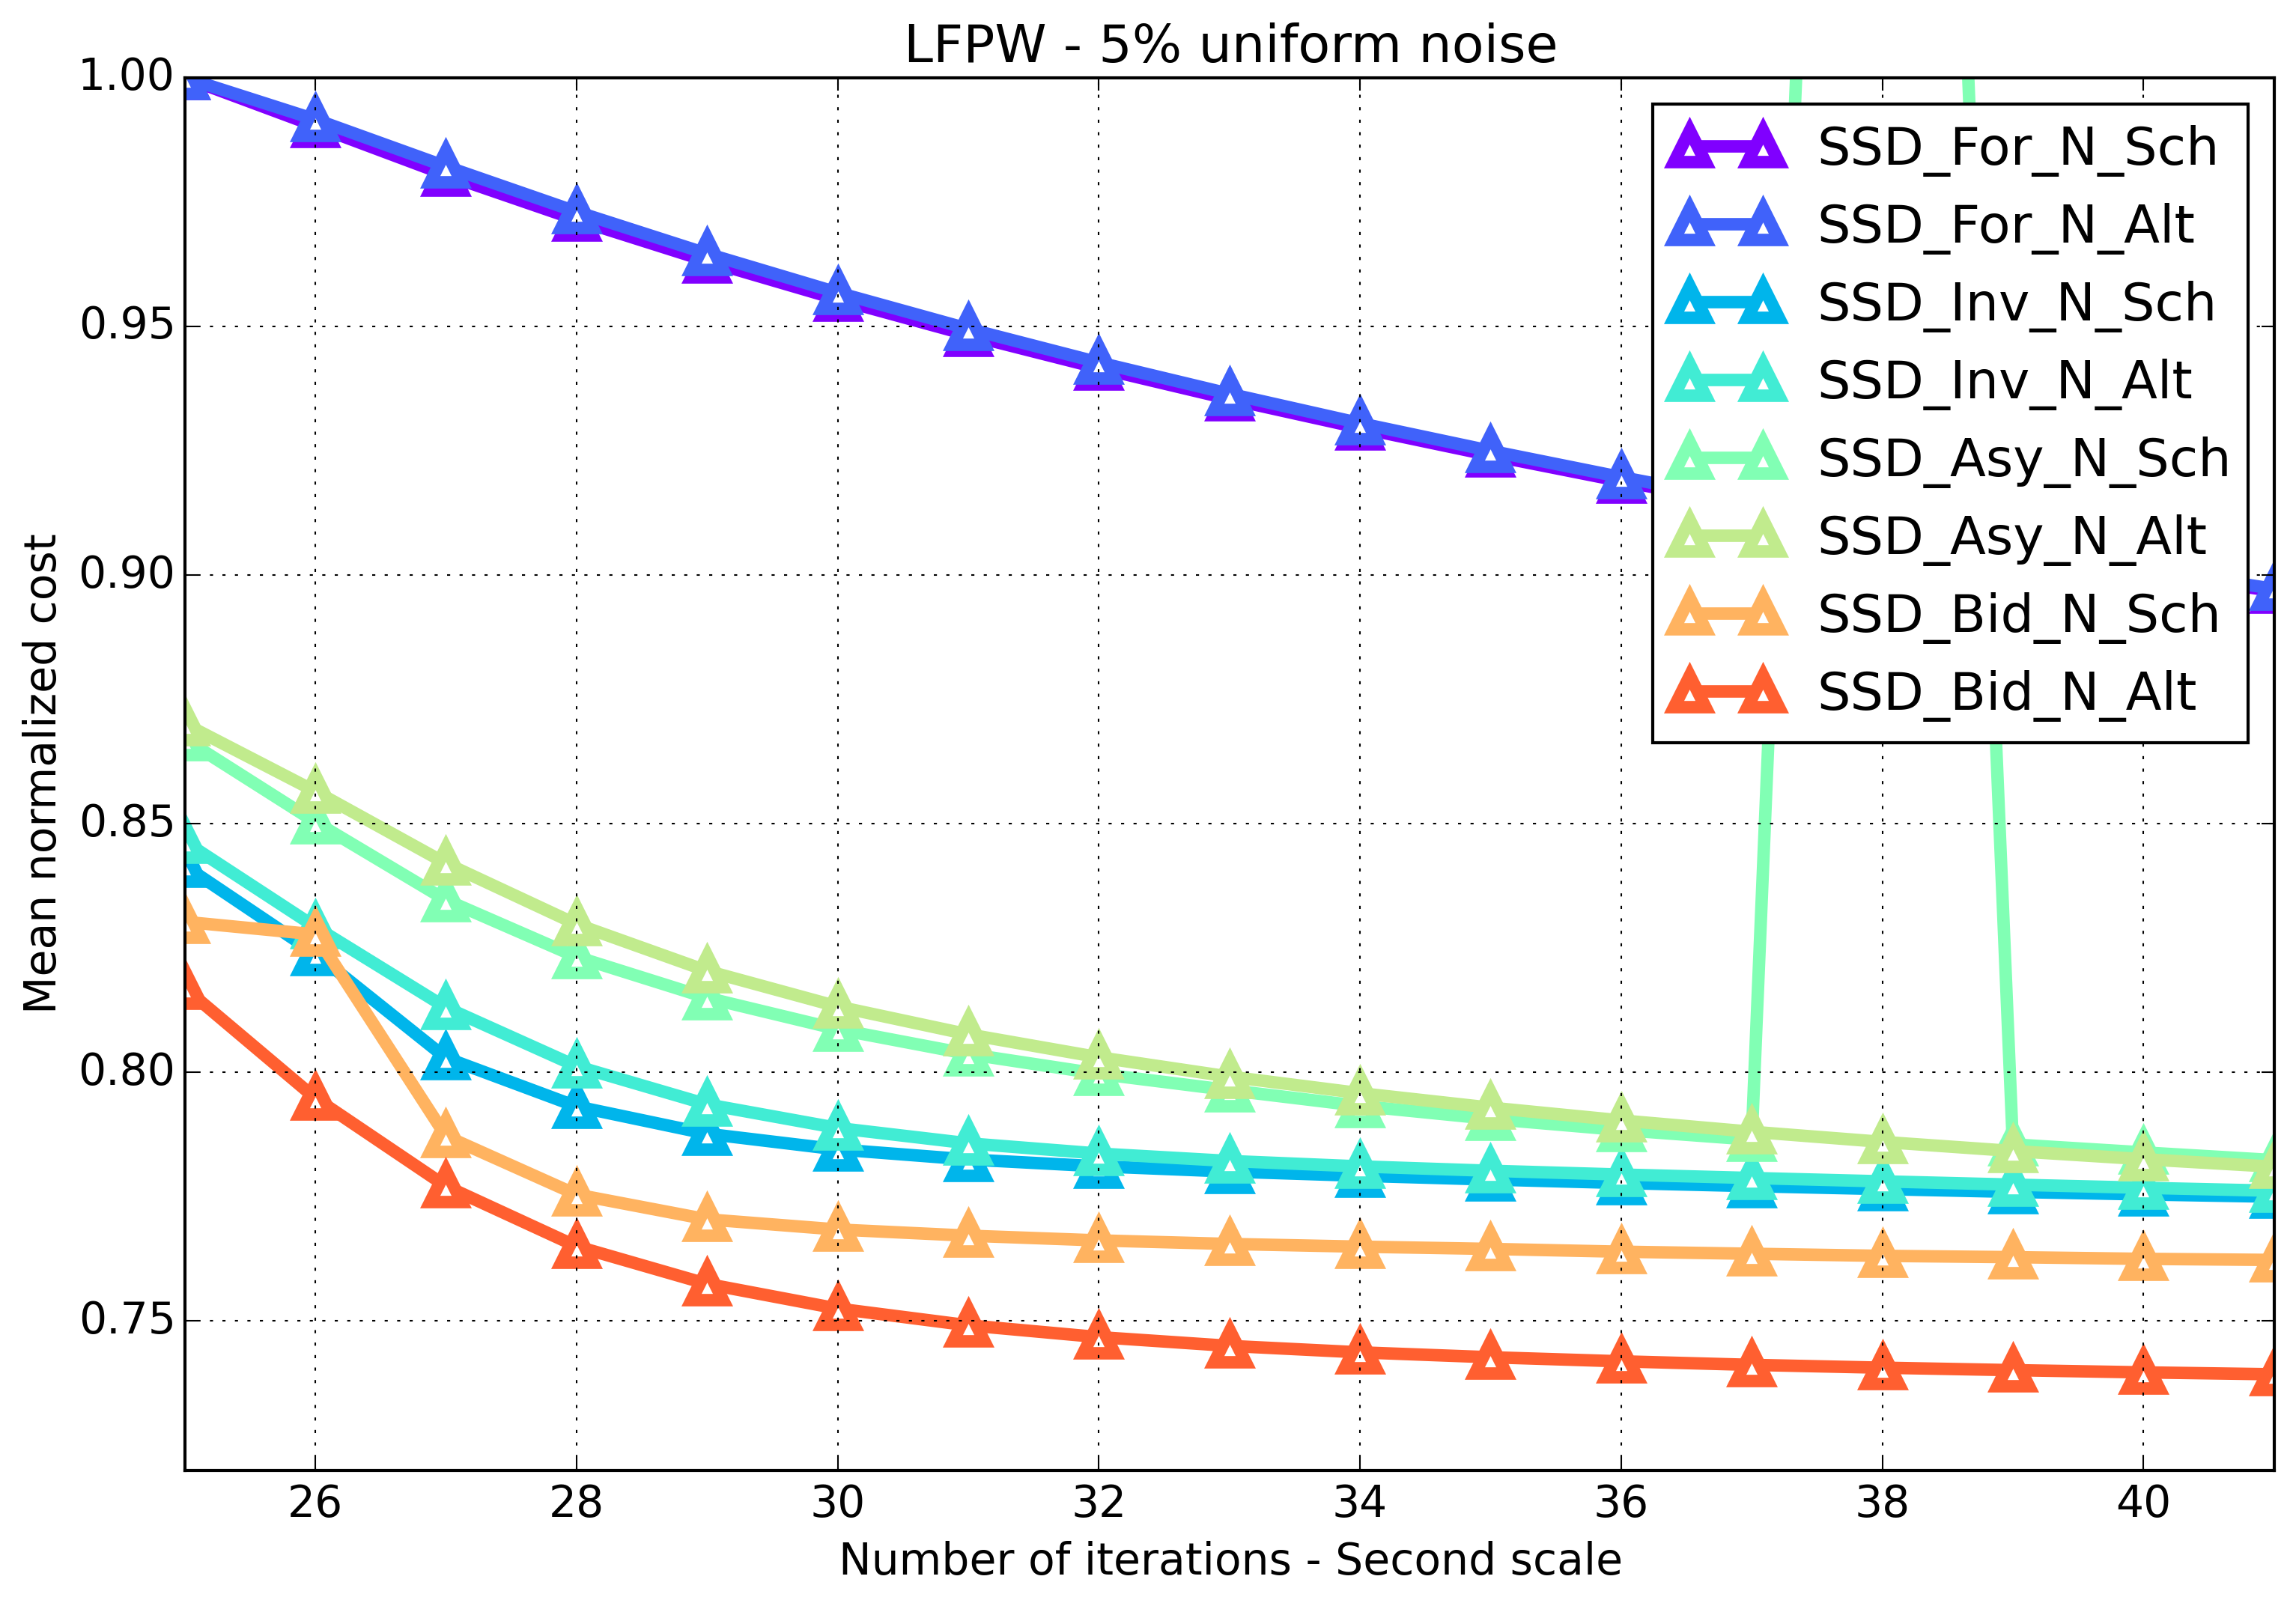
\includegraphics[width=\textwidth]{experiments/algorithms/ssd_n/mean_cost_vs_iters2_ssd_n_5.png}
	    \caption{Mean normalized cost vs number of second scale iterations on the LFPW test dataset for all SSD Newton algorithms initialized with $5\%$ uniform noise.}
	    \label{fig:mean_cost_vs_iters2_ssd_n_5}
	\end{subfigure}
	\par\bigskip\bigskip
	\begin{subfigure}{\textwidth}
		\center
		\begin{tabular}{lcccccc}
			\toprule
		    Algorithm & $<0.02$ & $<0.03$ & $<0.04$ & Mean & Sdt & Median 
		    \\
		    \midrule
		    Initialization & 0.000 & 0.004 & 0.055 & 0.080 & 0.028 & 0.078
		    \\
		    SSD\_For\_N\_Sch & 0.249 & 0.479 & 0.603 & 0.044 & 0.033 & 0.031
		    \\
		    SSD\_For\_N\_Alt & 0.244 & 0.476 & 0.600 & 0.044 & 0.033 & 0.032
		    \\
		    SSD\_Inv\_N\_Sch & 0.626 & 0.876 & 0.909 & 0.024 & 0.022 & \textbf{0.018}
		    \\
		    SSD\_Inv\_N\_Alt & 0.613 & 0.876 & 0.909 & 0.024 & 0.022 & \textbf{0.018}
		    \\
		    SSD\_Asy\_N\_Sch & 0.562 & 0.812 & 0.863 & 0.030 & 0.076 & 0.019
		    \\
		    SSD\_Asy\_N\_Alt & 0.557 & 0.808 & 0.862 & 0.027 & 0.025 & 0.019
		    \\
		    SSD\_Bid\_N\_Sch & \textbf{0.641} & 0.897 & 0.932 & \textbf{0.023} & 0.022 & \textbf{0.018}
		    \\
		    SSD\_Bid\_N\_Alt & 0.600 & \textbf{0.903} & \textbf{0.939} & \textbf{0.023} & \textbf{0.021} & \textbf{0.018}
		    \\
		    \bottomrule
	  	\end{tabular}
	  	\caption{Table showing the proportion of images fitted with a normalized point-to-point error below $0.02$, $0.03$ and $0.04$ together with the normalized point-to-point error Mean, Std and Median for all SSD Newton algorithms initialized with $5\%$ uniform noise.}
	    \label{tab:stats_ssd_n_5}
	\end{subfigure}
	\caption{Results showing the fitting accuracy and convergence properties of the SSD Newton algorithms on the LFPW test dataset initialized with $5\%$ uniform noise.}
	\label{fig:ssd_n_5}
\end{figure*}


\begin{figure*}[p]
	\centering
	\begin{subfigure}{0.48\textwidth}
	    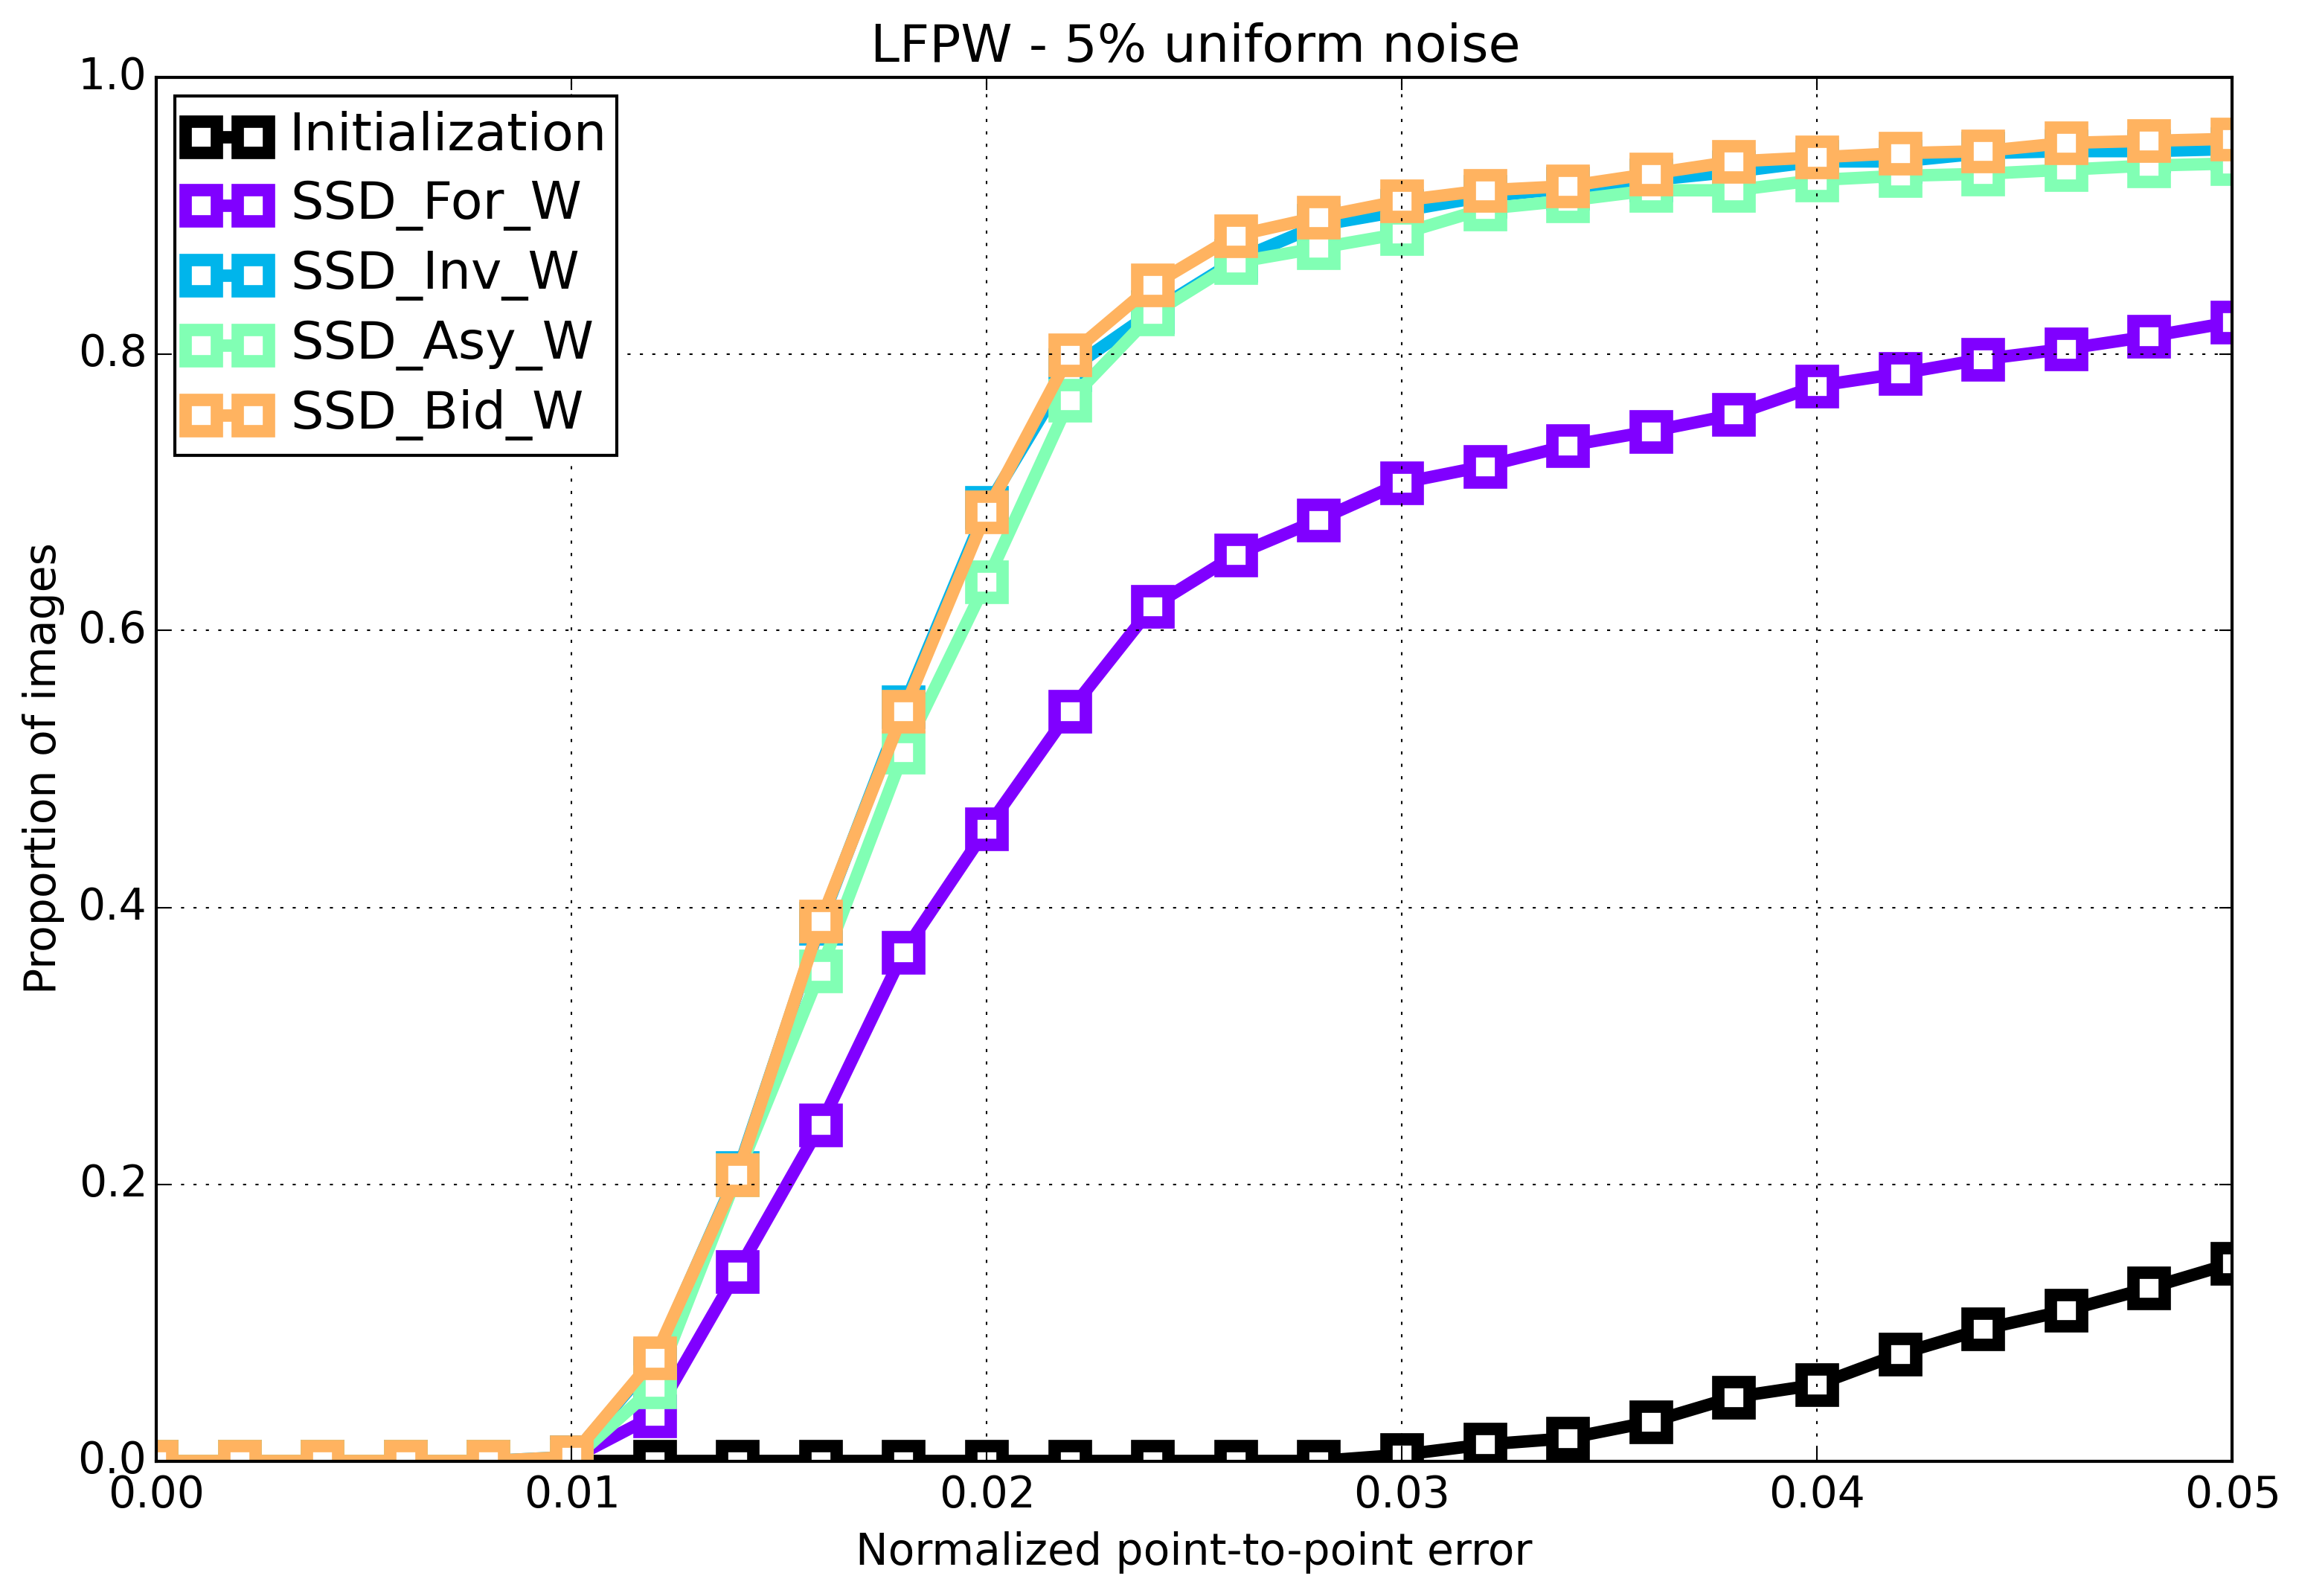
\includegraphics[width=\textwidth]{experiments/algorithms/ssd_w/ced_ssd_w_5.png}
	    \caption{CED on the LFPW test dataset for all SSD Wiberg algorithms initialized with $5\%$ uniform noise.}
	    \label{fig:ced_ssd_w_5}
	\end{subfigure}
	\hfill
	\begin{subfigure}{0.48\textwidth}
	    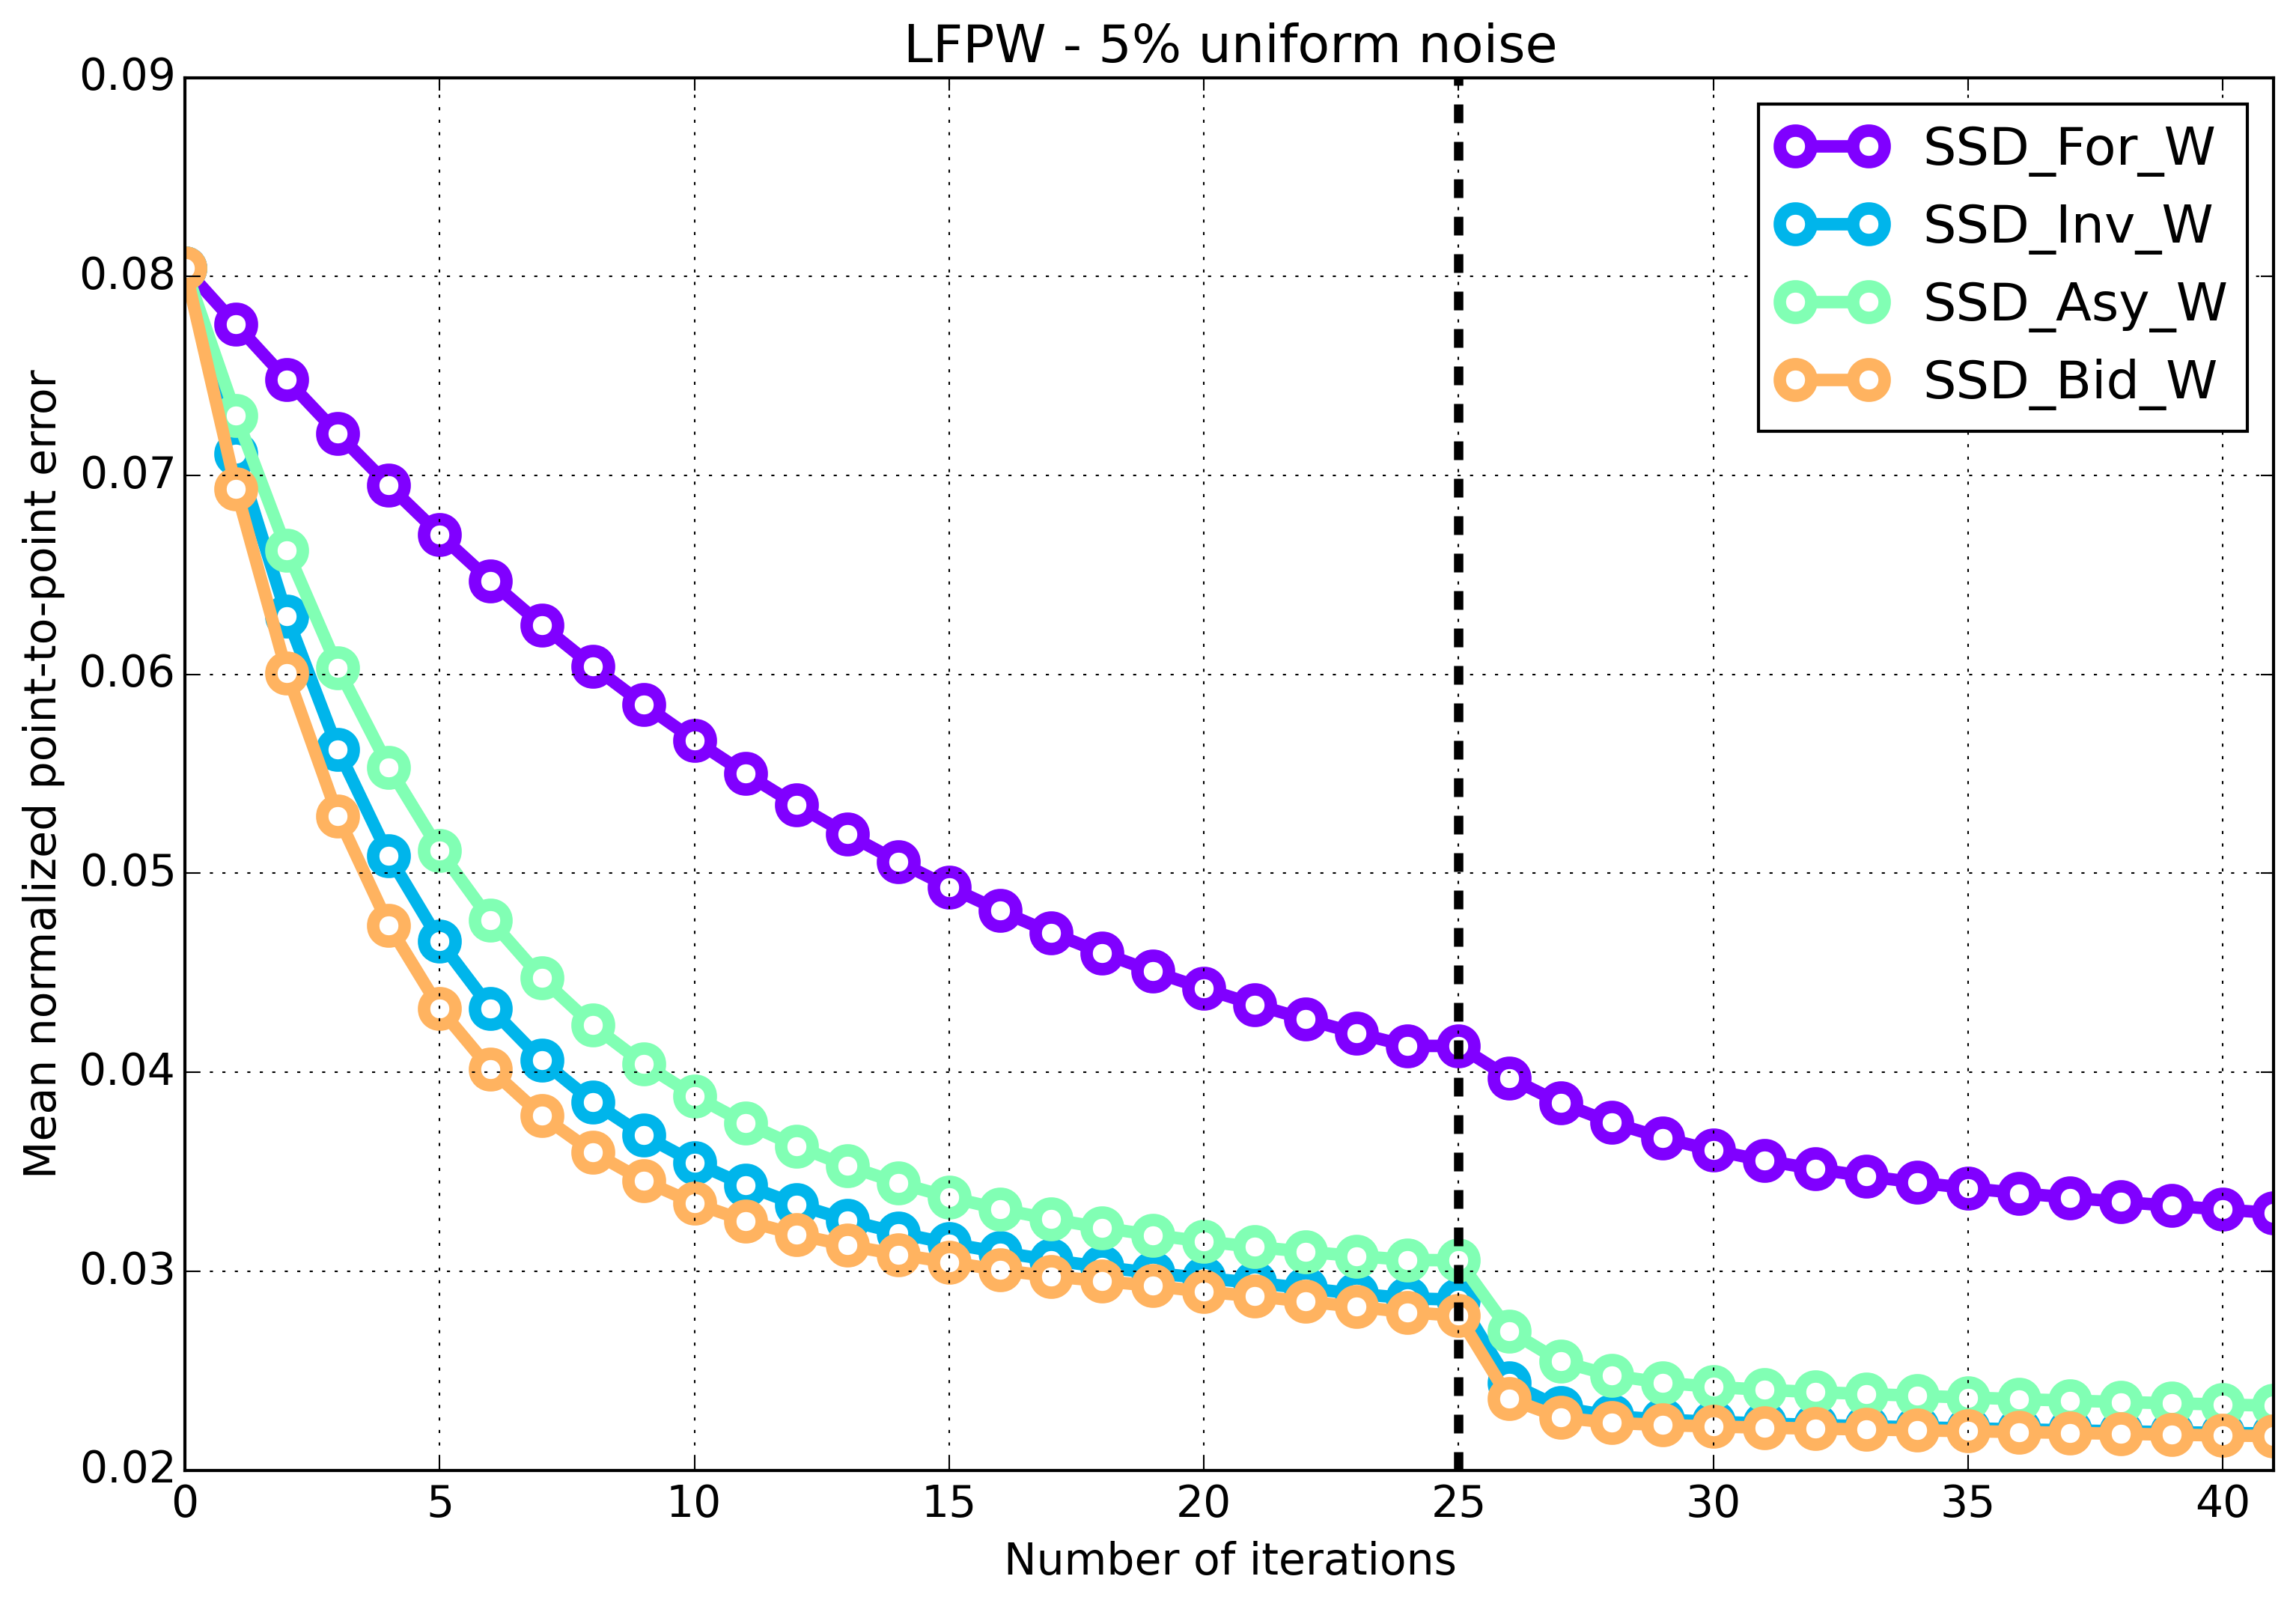
\includegraphics[width=\textwidth]{experiments/algorithms/ssd_w/mean_error_vs_iters_ssd_w_5.png}
	    \caption{Mean normalized point-to-point error vs number of iterations on the LFPW test dataset for all SSD Wiberg algorithms initialized with $5\%$ uniform noise.}
	    \label{fig:mean_error_vs_iters_ssd_w_5}
	\end{subfigure}
	\par\bigskip\bigskip
	\begin{subfigure}{0.48\textwidth}
	    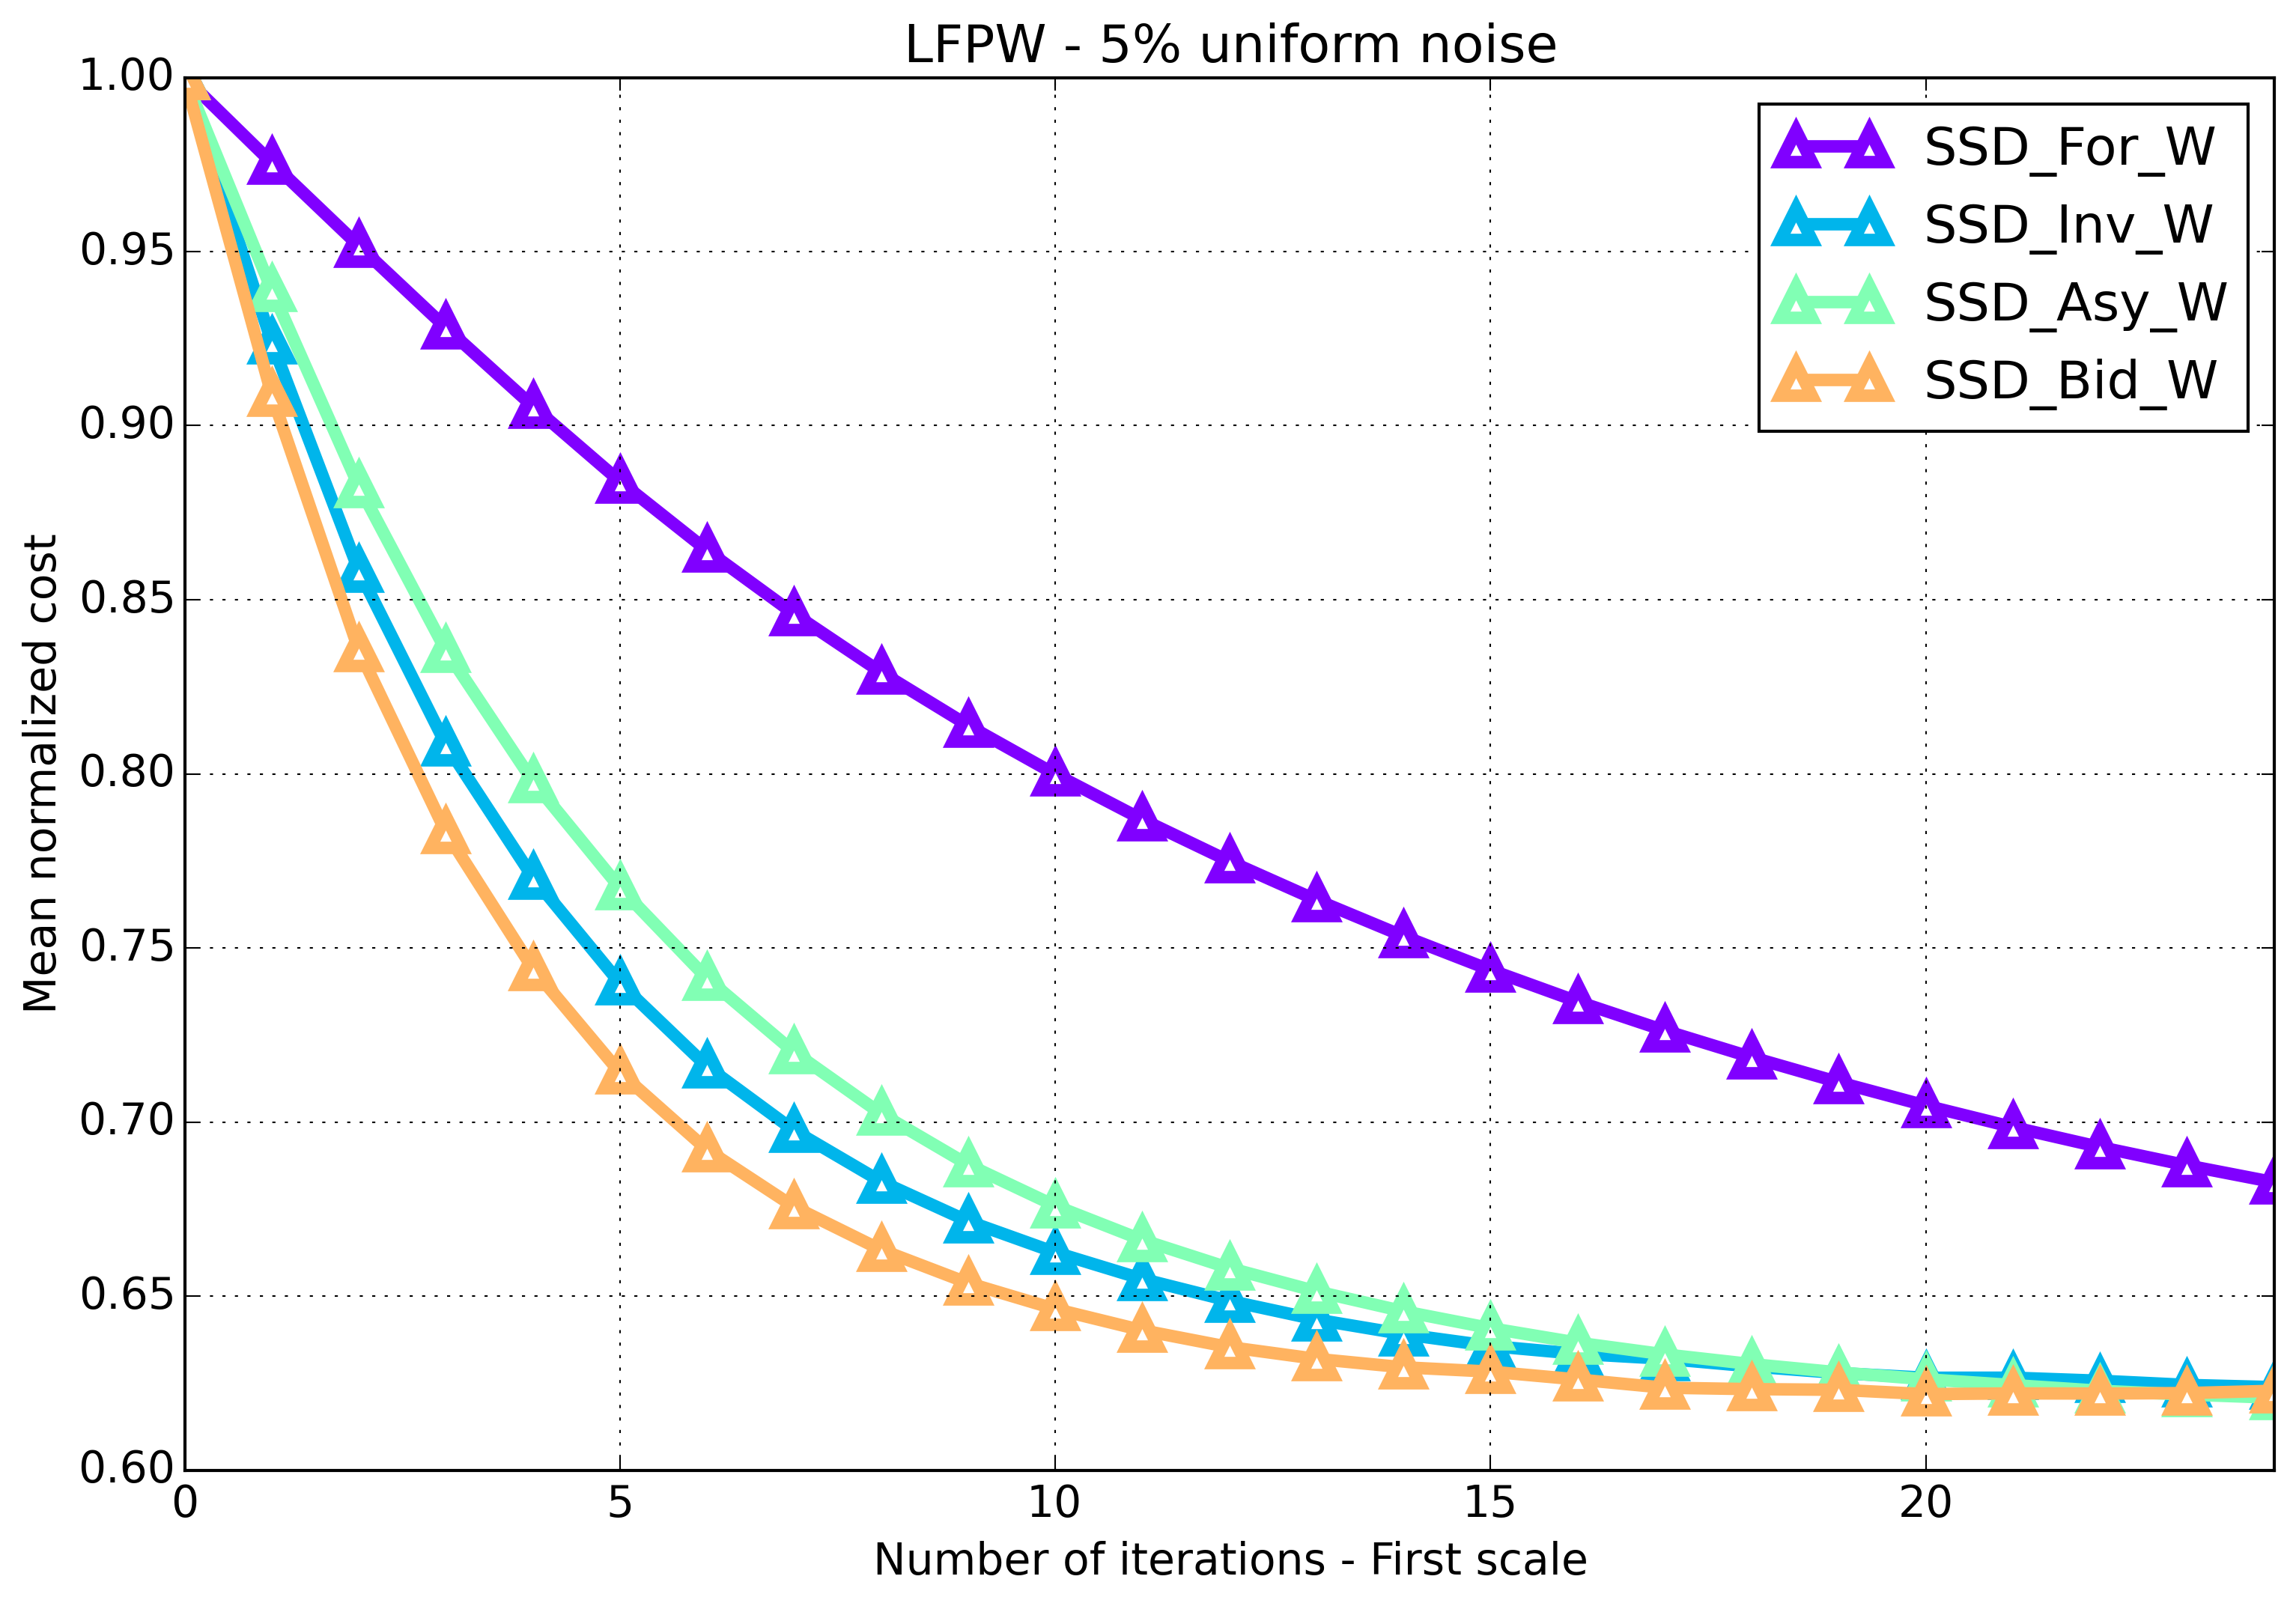
\includegraphics[width=\textwidth]{experiments/algorithms/ssd_w/mean_cost_vs_iters1_ssd_w_5.png}
	    \caption{Mean normalized cost vs number of first scale iterations on the LFPW test dataset for all SSD Wiberg algorithms initialized with $5\%$ uniform noise.}
	    \label{fig:mean_cost_vs_iters1_ssd_w_5}
	\end{subfigure}
	\hfill
	\begin{subfigure}{0.48\textwidth}
	    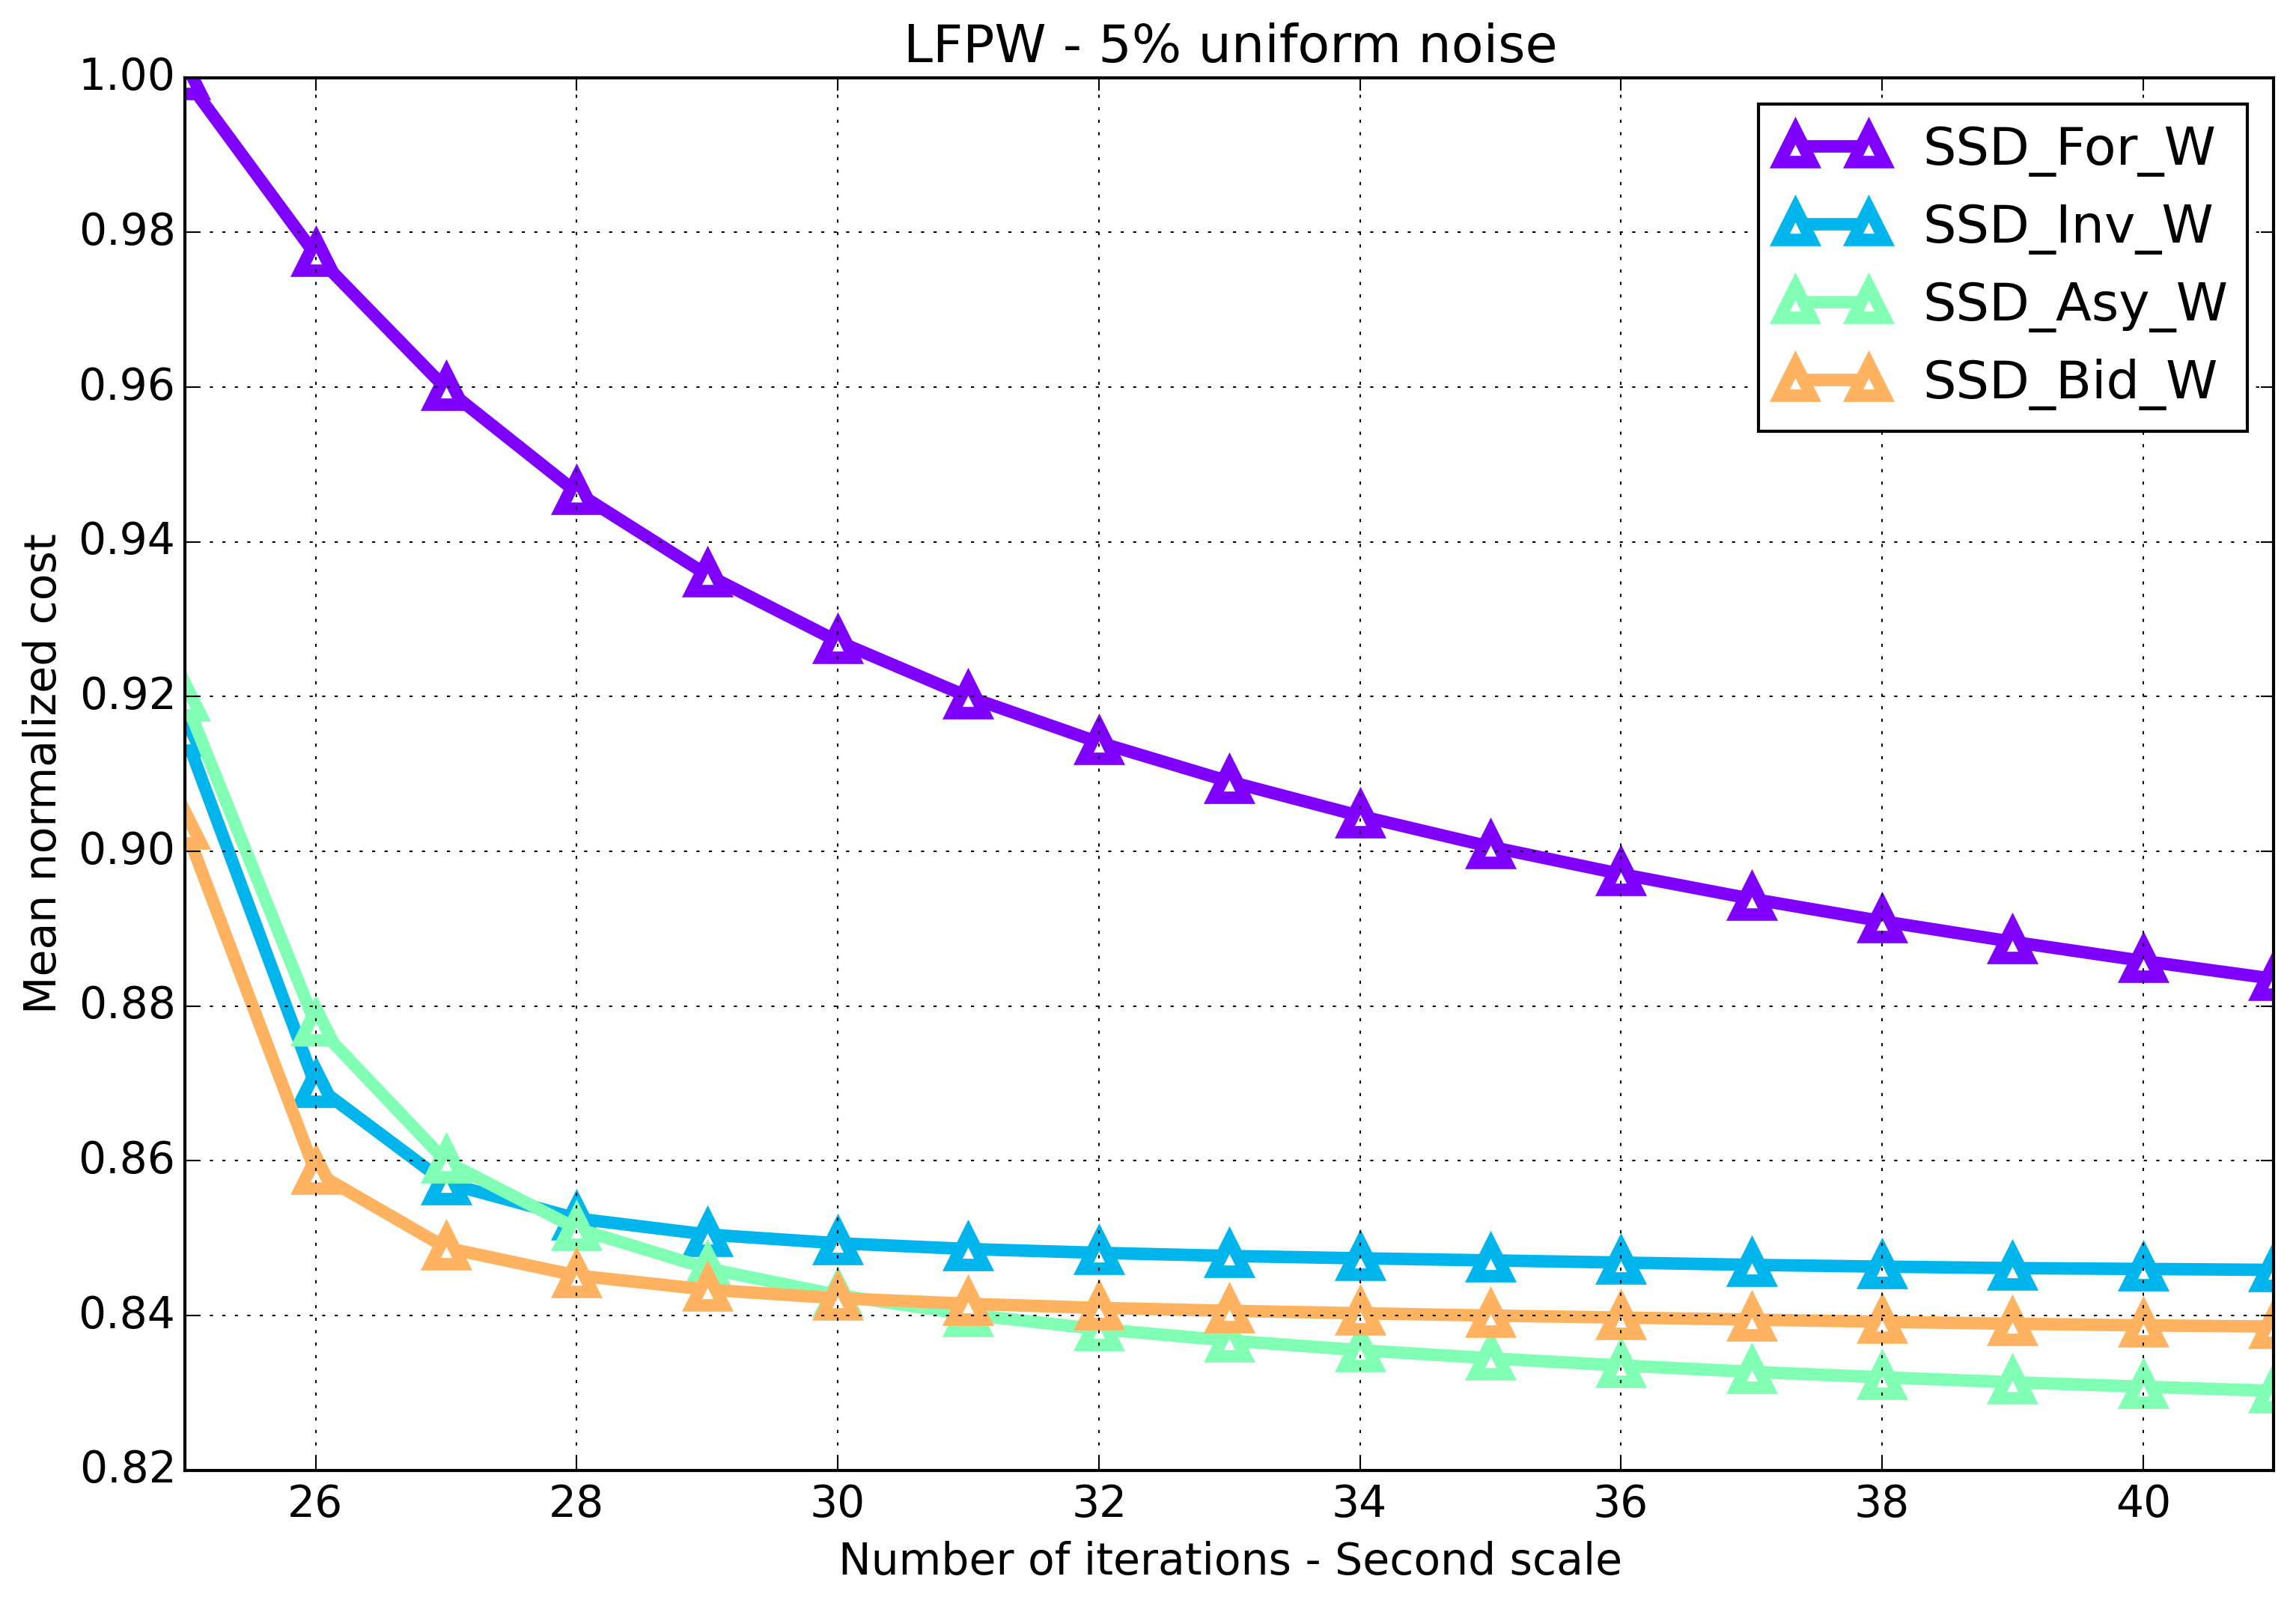
\includegraphics[width=\textwidth]{experiments/algorithms/ssd_w/mean_cost_vs_iters2_ssd_w_5.png}
	    \caption{Mean normalized cost vs number of second scale iterations on the LFPW test dataset for all SSD Wiberg algorithms initialized with $5\%$ uniform noise.}
	    \label{fig:mean_cost_vs_iters2_ssd_w_5}
	\end{subfigure}
	\par\bigskip\bigskip
	\begin{subfigure}{\textwidth}
		\center
		\begin{tabular}{lcccccc}
		    \toprule
		    Algorithm & $<0.02$ & $<0.03$ & $<0.04$ & Mean & Sdt & Median 
		    \\
		    \midrule
		    Initialization & 0.000 & 0.004 & 0.055 & 0.080 & 0.028 & 0.078
		    \\ 
		    SSD\_For\_W & 0.457 & 0.707 & 0.777 & 0.33 & 0.030 & 0.021
		    \\
		    SSD\_Inv\_W & \textbf{0.689} & 0.903 & 0.939 & \textbf{0.22} & \textbf{0.019} & \textbf{0.017}
		    \\
		    SSD\_Asy\_W & 0.635 & 0.887 & 0.926 & 0.23 & 0.021 & 0.018
		    \\
		    SSD\_Bid\_W & 0.686 & \textbf{0.911} & \textbf{0.942} & \textbf{0.22} & \textbf{0.019} & \textbf{0.017}
		    \\
		    \bottomrule
	  	\end{tabular}
	  	\caption{Table showing the proportion of images fitted with a normalized point-to-point error below $0.02$, $0.03$ and $0.04$ together with the normalized point-to-point error Mean, Std and Median for all SSD Wiberg algorithms initialized with $5\%$ uniform noise.}
	    \label{tab:stats_ssd_w_5}
	\end{subfigure}
	\caption{Results showing the fitting accuracy and convergence properties of the SSD Wiberg algorithms on the LFPW test dataset.}
	\label{fig:ssd_w_5}
\end{figure*}


\subsubsection{BPO Gauss-Newton algorithms}

Results for \emph{BPO Gauss-Newton} algorithms are reported on Figure \ref{fig:bpo_gn_5}. We can observe that, there is significant drop in accuracy for \emph{Inverse} and \emph{Bidirectional} algorithms with respect to their \emph{SSD} version, \ref{fig:ced_bpo_gn_5} and Table \ref{tab:stats_bpo_gn_5}. As expected, the \emph{Forward} algorithm achieves virtually the same results as its \emph{SSD} counterpart. The \emph{Asymmetric} algorithm obtains similar accuracy to that of the best performing \emph{SSD} algorithms.

Looking at Figures \ref{fig:mean_error_vs_iters_bpo_gn_5}, \ref{fig:mean_cost_vs_iters1_bpo_gn_5} and \ref{fig:mean_cost_vs_iters2_bpo_gn_5} we can see that \emph{Inverse} and \emph{Bidirectional} algorithms converge slightly faster than the \emph{Asymmetric} algorithm. However, the \emph{Asymmetric} algorithm ends descending to a significant lower value of the mean normalized cost which also translates to a lower value for the final mean normalized point-to-point error. Similar to \emph{SSD} algorithms, the \emph{Forward} algorithm  is the worst convergent algorithm.

Finally notice that, in this case, there is virtually no difference, in accuracy and speed of convergence, between the \emph{Simultaneous Schur} and \emph{Alternated} optimizations strategies used by the \emph{Bidirectional} algorithm.


\subsubsection{BPO Newton algorithms}

Results for \emph{BPO Newton} algorithms are reported on Figure \ref{fig:bpo_n_5}. It can be clearly seen that BPO Newton algorithms perform much worse than their Gauss-Newton and SSD counterparts. The final fitting accuracy obtained by these algorithms is very poor compared to the one obtained by the best \emph{SSD} and \emph{BPO Gauss-Newton} algorithms, Figures \ref{fig:ced_bpo_n_5} and Table \ref{tab:stats_bpo_n_5}. In fact, by looking at Figures \ref{fig:mean_error_vs_iters_bpo_n_5}, \ref{fig:mean_cost_vs_iters1_bpo_n_5} and \ref{fig:mean_cost_vs_iters2_bpo_n_5} only the \emph{Forward} and \emph{Asymmetric} algorithms seem to be stable at the second level of the Gaussian pyramid with \emph{Inverse} and \emph{Bidirectional} algorithms completely diverging in for some of the images as shown by the large mean and std of their final normalized point-to-point errors. 


\subsubsection{BPO Wiberg algorithms}

Results for the \emph{BPO Bidirectional Wiberg} algorithm are reported on Figure \ref{fig:bpo_n_5}. As expected, the results are virtually identical to those of the obtained by \emph{BPO Bidirectional Gauss-Newton} algorithms.  


\begin{figure*}[p]
	\centering
	\begin{subfigure}{0.48\textwidth}
	    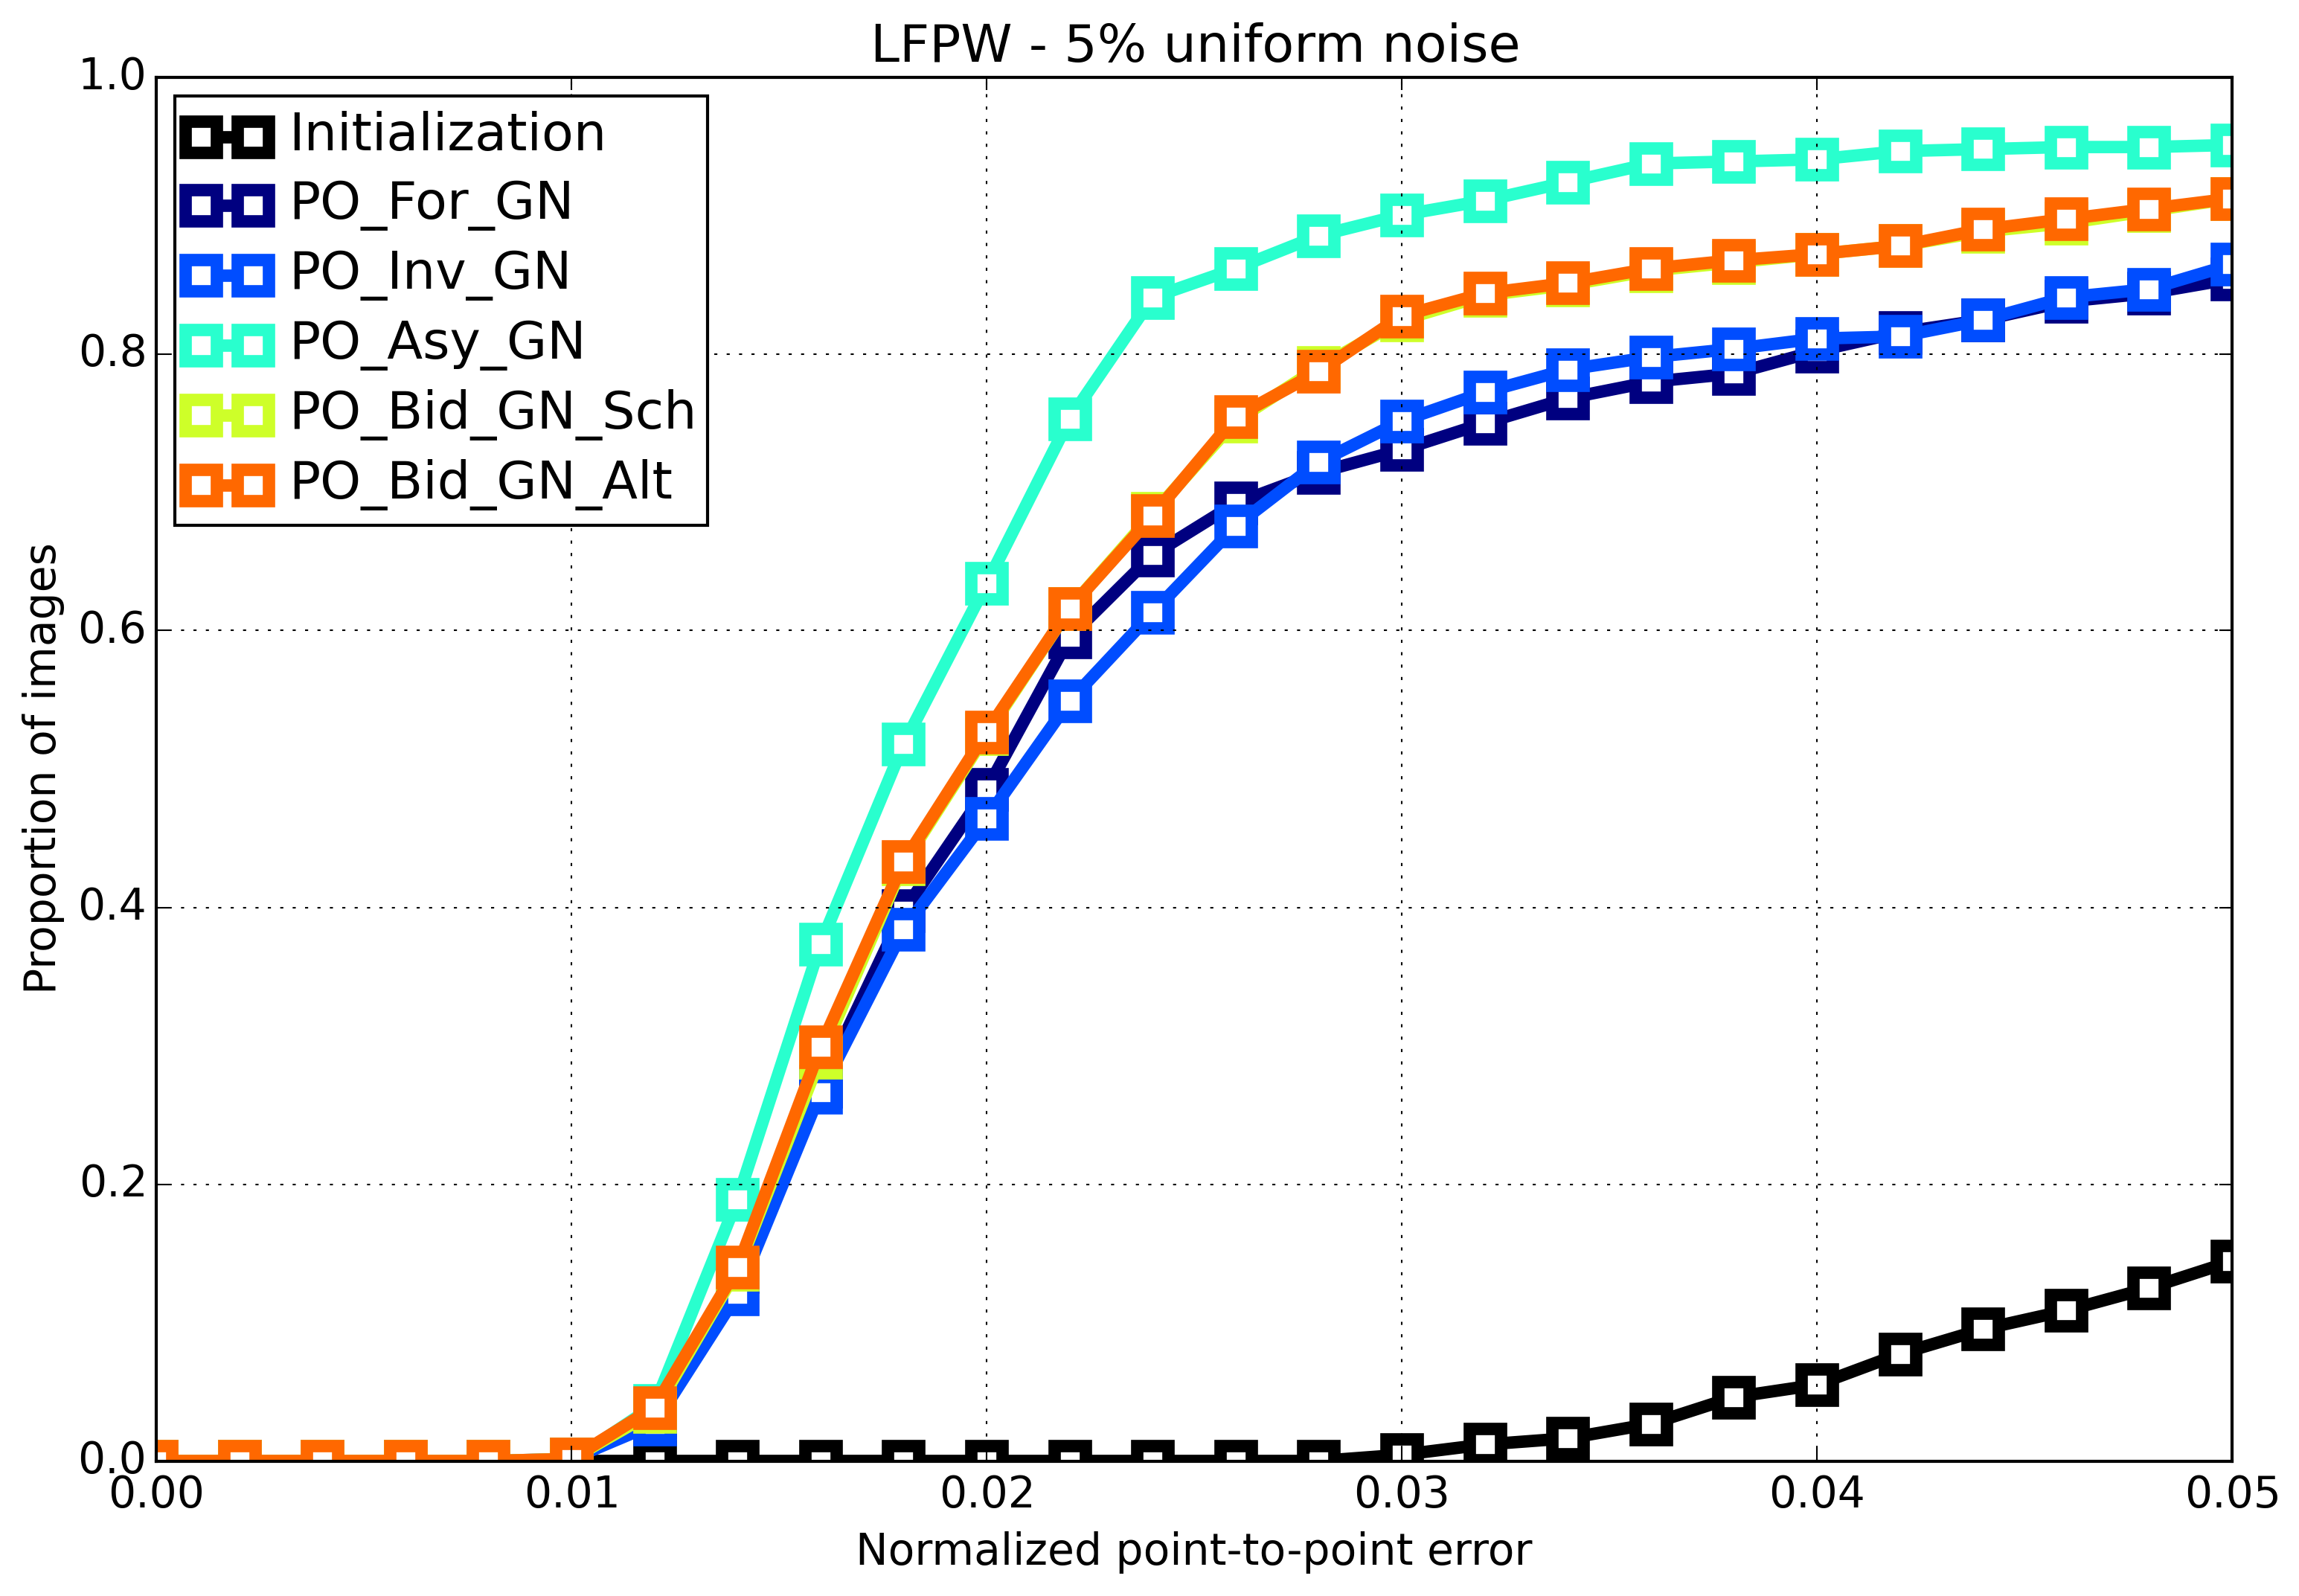
\includegraphics[width=\textwidth]{experiments/algorithms/po_gn/ced_po_gn_5.png}
	    \caption{CED graph on the LFPW test dataset for all Project-Out Gauss-Newton algorithms initialized with $5\%$ uniform noise.}
	    \label{fig:ced_bpo_gn_5}
	\end{subfigure}
	\hfill
	\begin{subfigure}{0.48\textwidth}
	    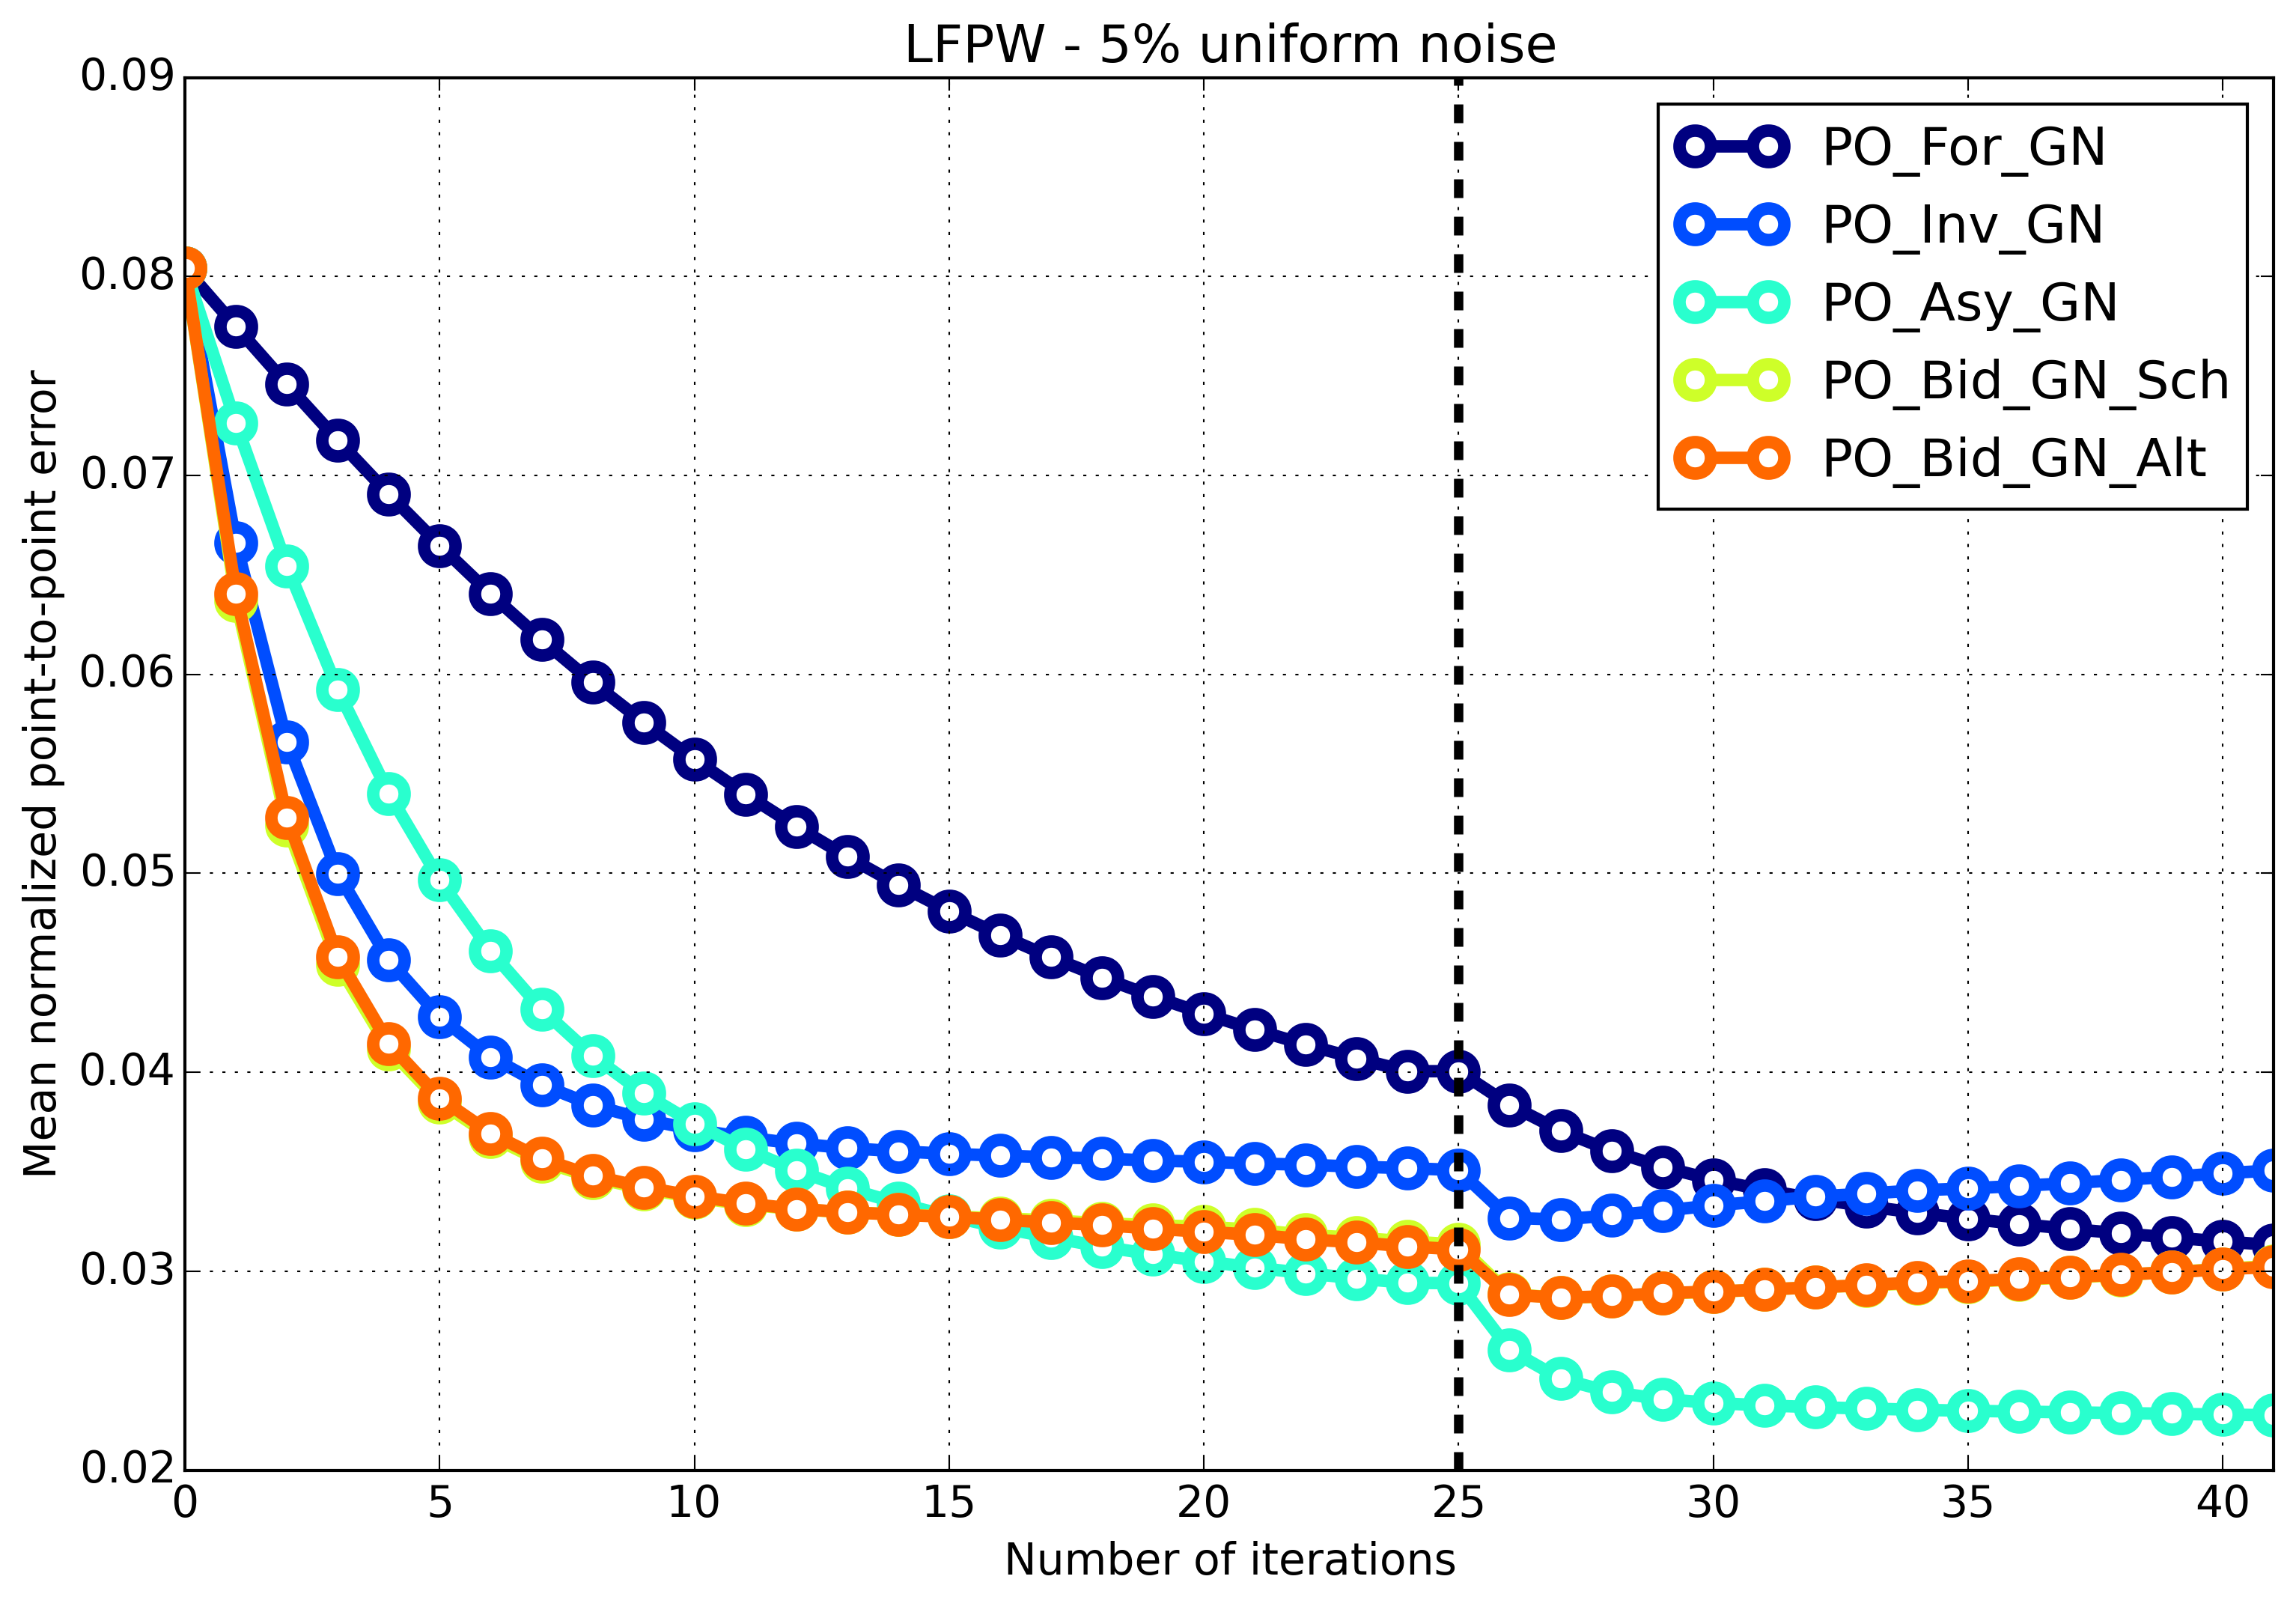
\includegraphics[width=\textwidth]{experiments/algorithms/po_gn/mean_error_vs_iters_po_gn_5.png}
	    \caption{Mean normalized point-to-point error vs number of iterations on the LFPW test dataset for all Project-Out Gauss-Newton algorithms initialized with $5\%$ uniform noise.}
	    \label{fig:mean_error_vs_iters_bpo_gn_5}
	\end{subfigure}
	\par\bigskip\bigskip
	\begin{subfigure}{0.48\textwidth}
	    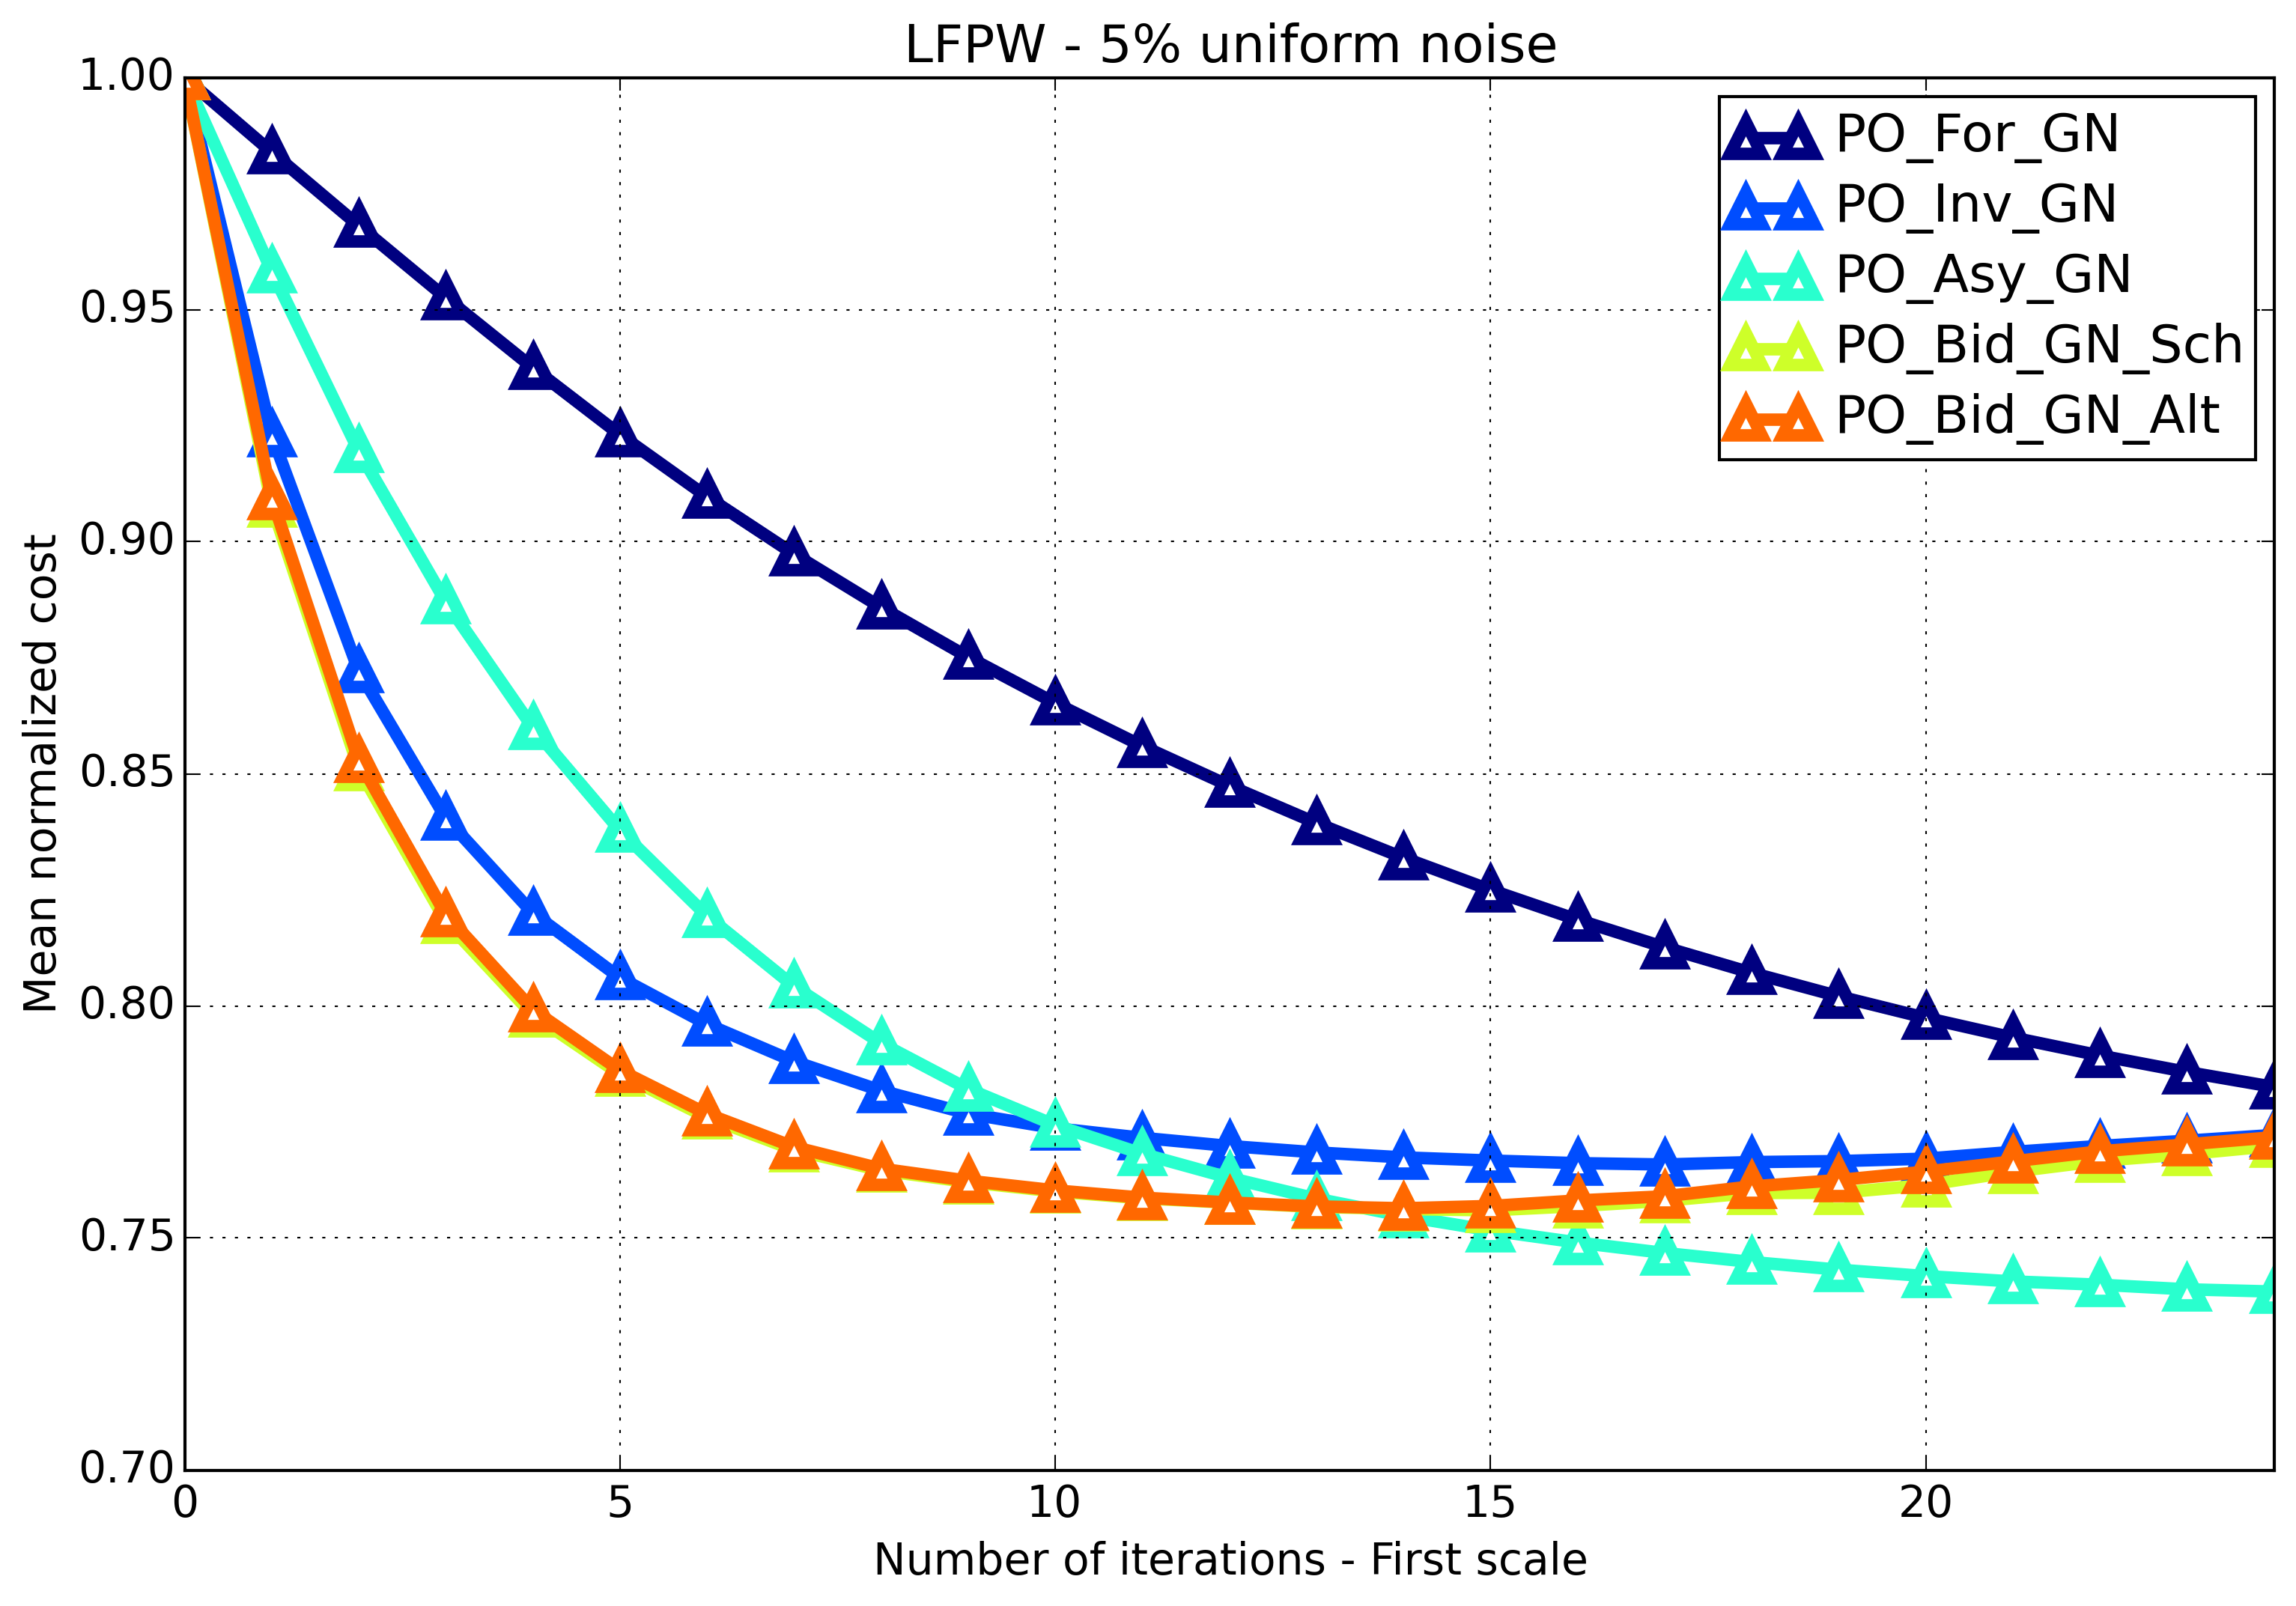
\includegraphics[width=\textwidth]{experiments/algorithms/po_gn/mean_cost_vs_iters1_po_gn_5.png}
	    \caption{Mean normalized cost vs number of first scale iterations on the LFPW test dataset for all Project-Out Gauss-Newton algorithms initialized with $5\%$ uniform noise.}
	    \label{fig:mean_cost_vs_iters1_bpo_gn_5}
	\end{subfigure}
	\hfill
	\begin{subfigure}{0.48\textwidth}
	    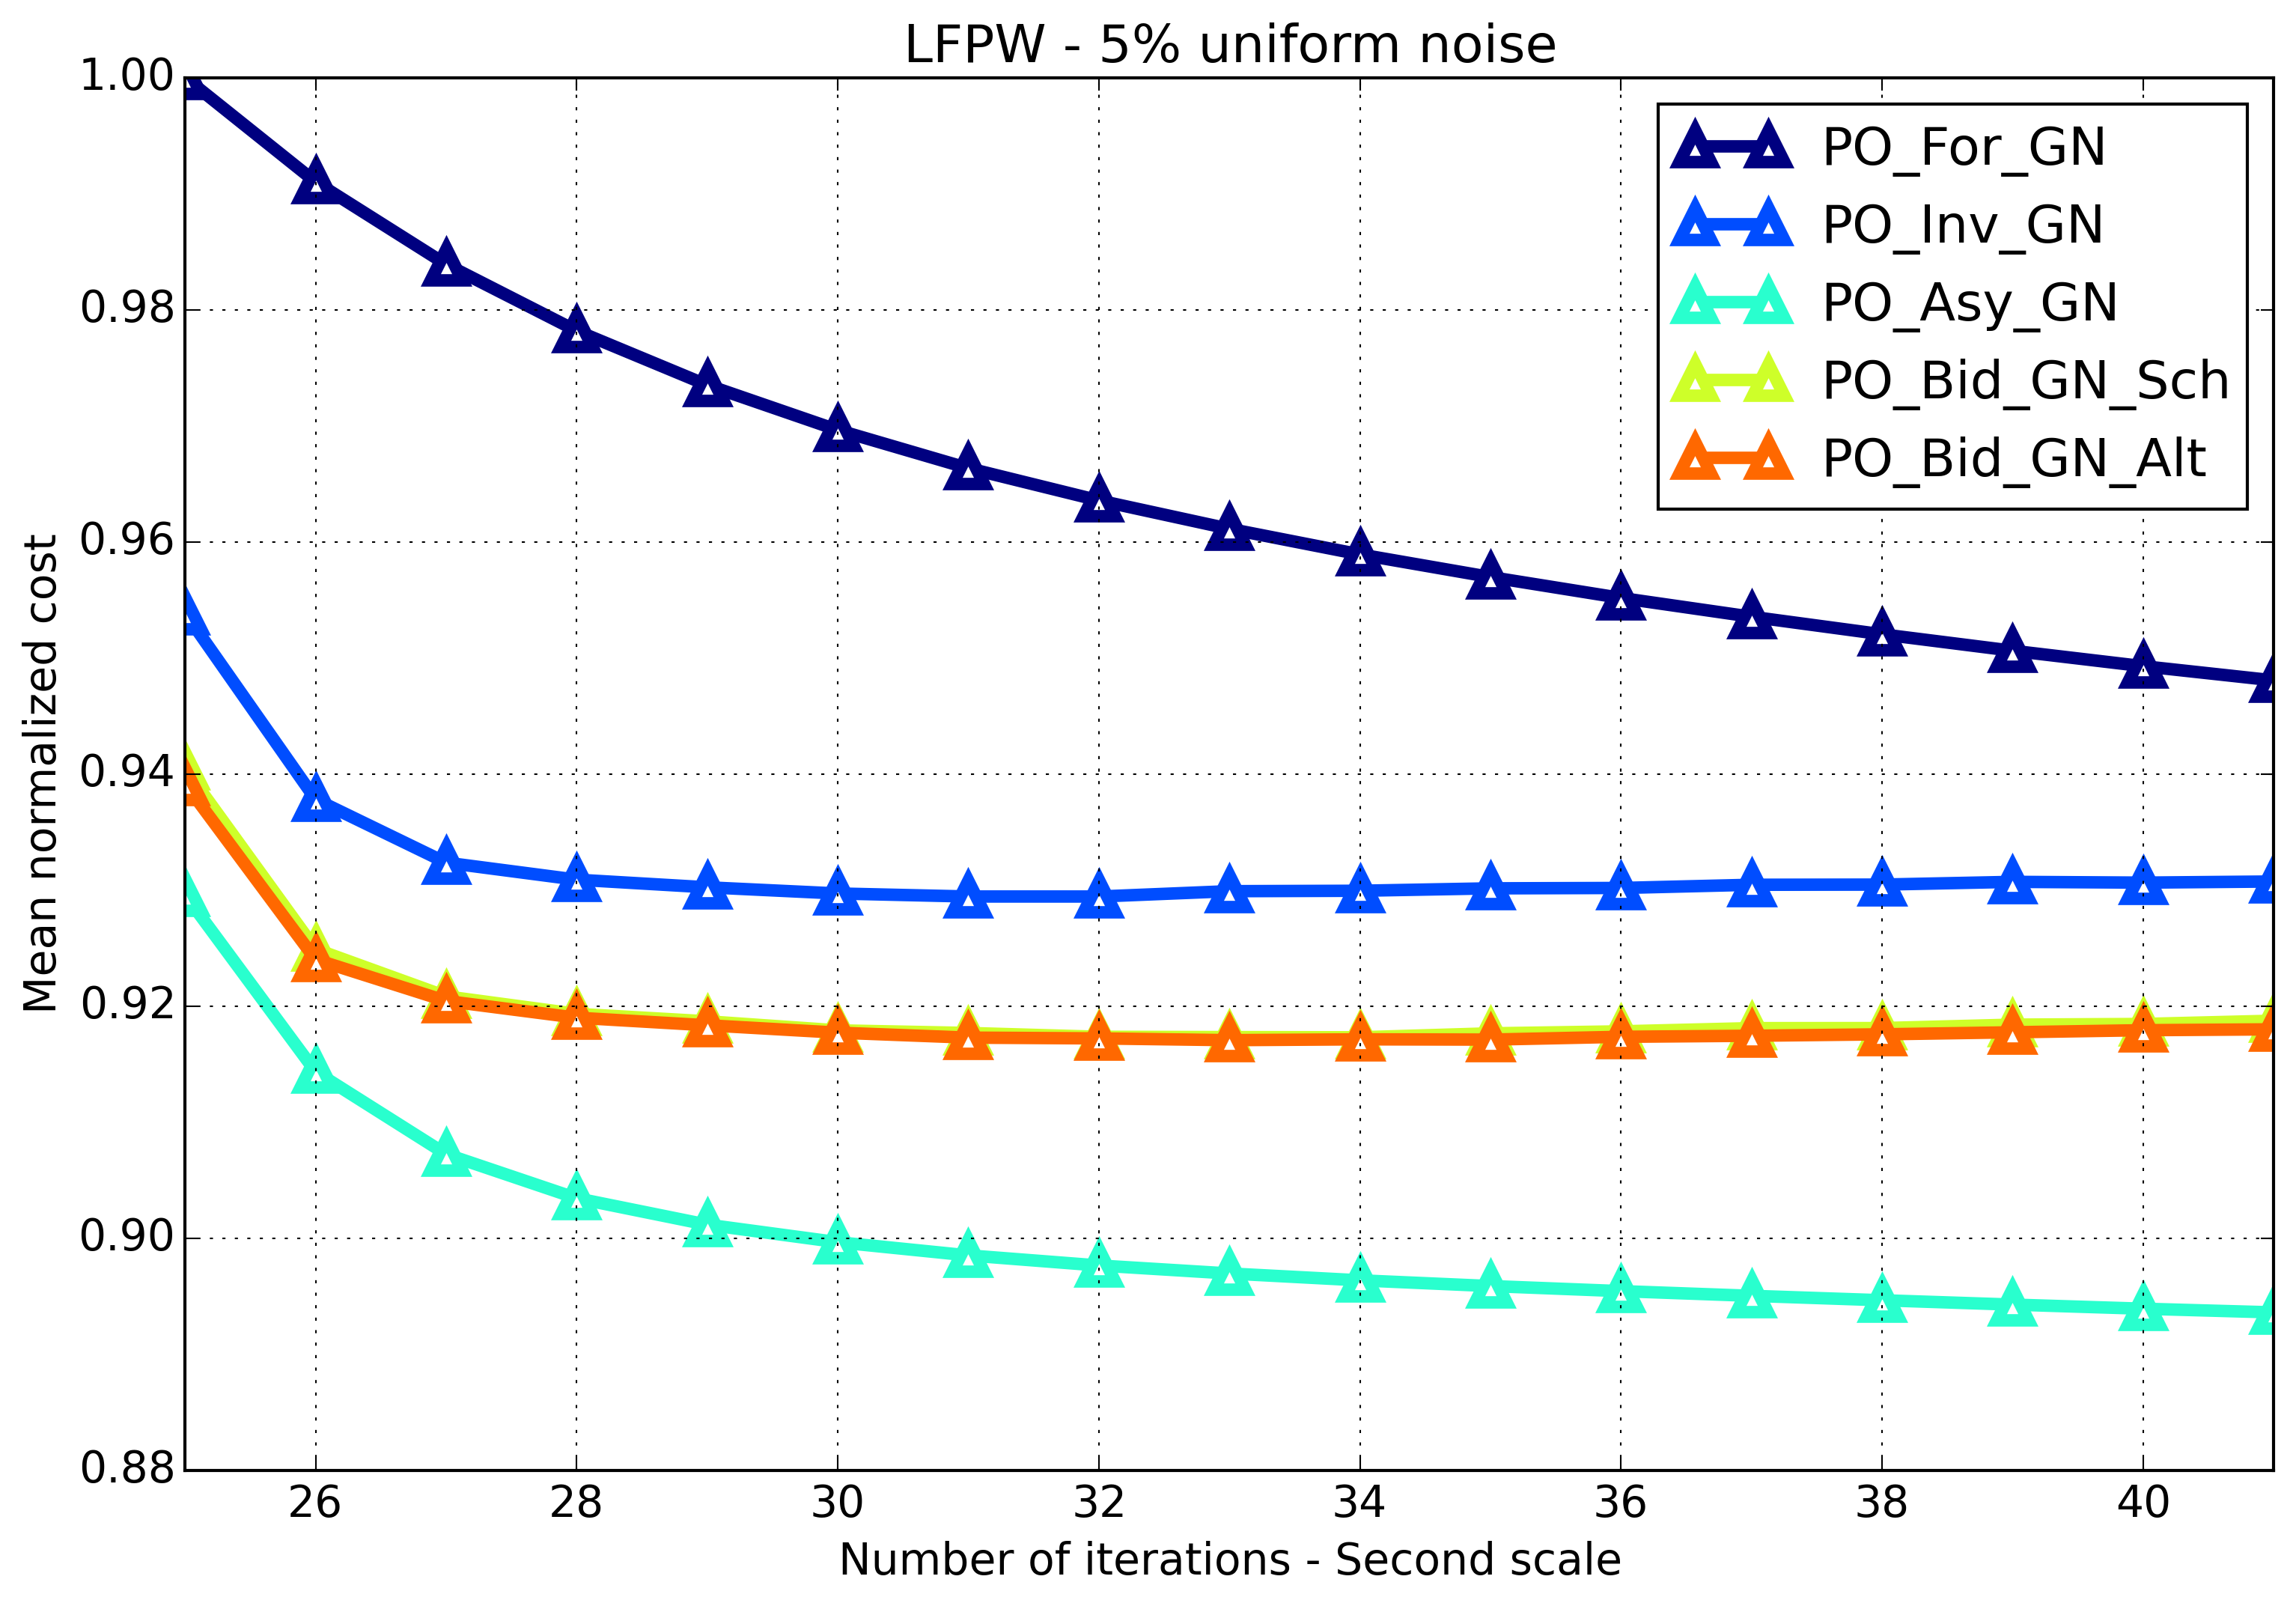
\includegraphics[width=\textwidth]{experiments/algorithms/po_gn/mean_cost_vs_iters2_po_gn_5.png}
	    \caption{Mean normalized cost vs number of second scale iterations on the LFPW test dataset for all Project-Out Gauss-Newton algorithms initialized with $5\%$ uniform noise.}
	    \label{fig:mean_cost_vs_iters2_bpo_gn_5}
	\end{subfigure}
	\par\bigskip\bigskip
	\begin{subfigure}{\textwidth}
		\center
		\begin{tabular}{lcccccc}
		    \toprule
		    Algorithm & $<0.02$ & $<0.03$ & $<0.04$ & Mean & Sdt & Median 
		    \\
		    \midrule
		    Initialization & 0.000 & 0.004 & 0.055 & 0.080 & 0.028 & 0.078
		    \\ 
		    PO\_For\_GN\_Sch & 0.470 & 0.729 & 0.799 & 0.031 & 0.029 & 0.021
		    \\
		    PO\_For\_GN\_Alt & 0.458 & 0.719 & 0.780 & 0.035 & 0.044 & 0.021
		    \\
		    PO\_Inv\_GN\_Sch & \textbf{0.637} & \textbf{0.891} & \textbf{0.938} & \textbf{0.023} & \textbf{0.021} & \textbf{0.018}
		    \\
		    PO\_Bid\_GN\_Sch & 0.528 & 0.802 & 0.862 & 0.030 & 0.039 & 0.020
		    \\
		    PO\_Bid\_GN\_Alt & 0.528 & 0.805 & 0.865 & 0.030 & 0.040 & 0.019
		    \\
		    \bottomrule
	  	\end{tabular}
	  	\caption{Table showing the proportion of images fitted with a normalized point-to-point error below $0.02$, $0.03$ and $0.04$ together with the normalized point-to-point error Mean, Std and Median for all Project-Out Gauss-Newton algorithms initialized with $5\%$ uniform noise.}
	    \label{tab:stats_bpo_gn_5}
	\end{subfigure}
	\caption{Results showing the fitting accuracy and convergence properties of the Project-Out Gauss-Newton algorithms on the LFPW test dataset.}
	\label{fig:bpo_gn_5}
\end{figure*}


\begin{figure*}[p]
	\centering
	\begin{subfigure}{0.48\textwidth}
	    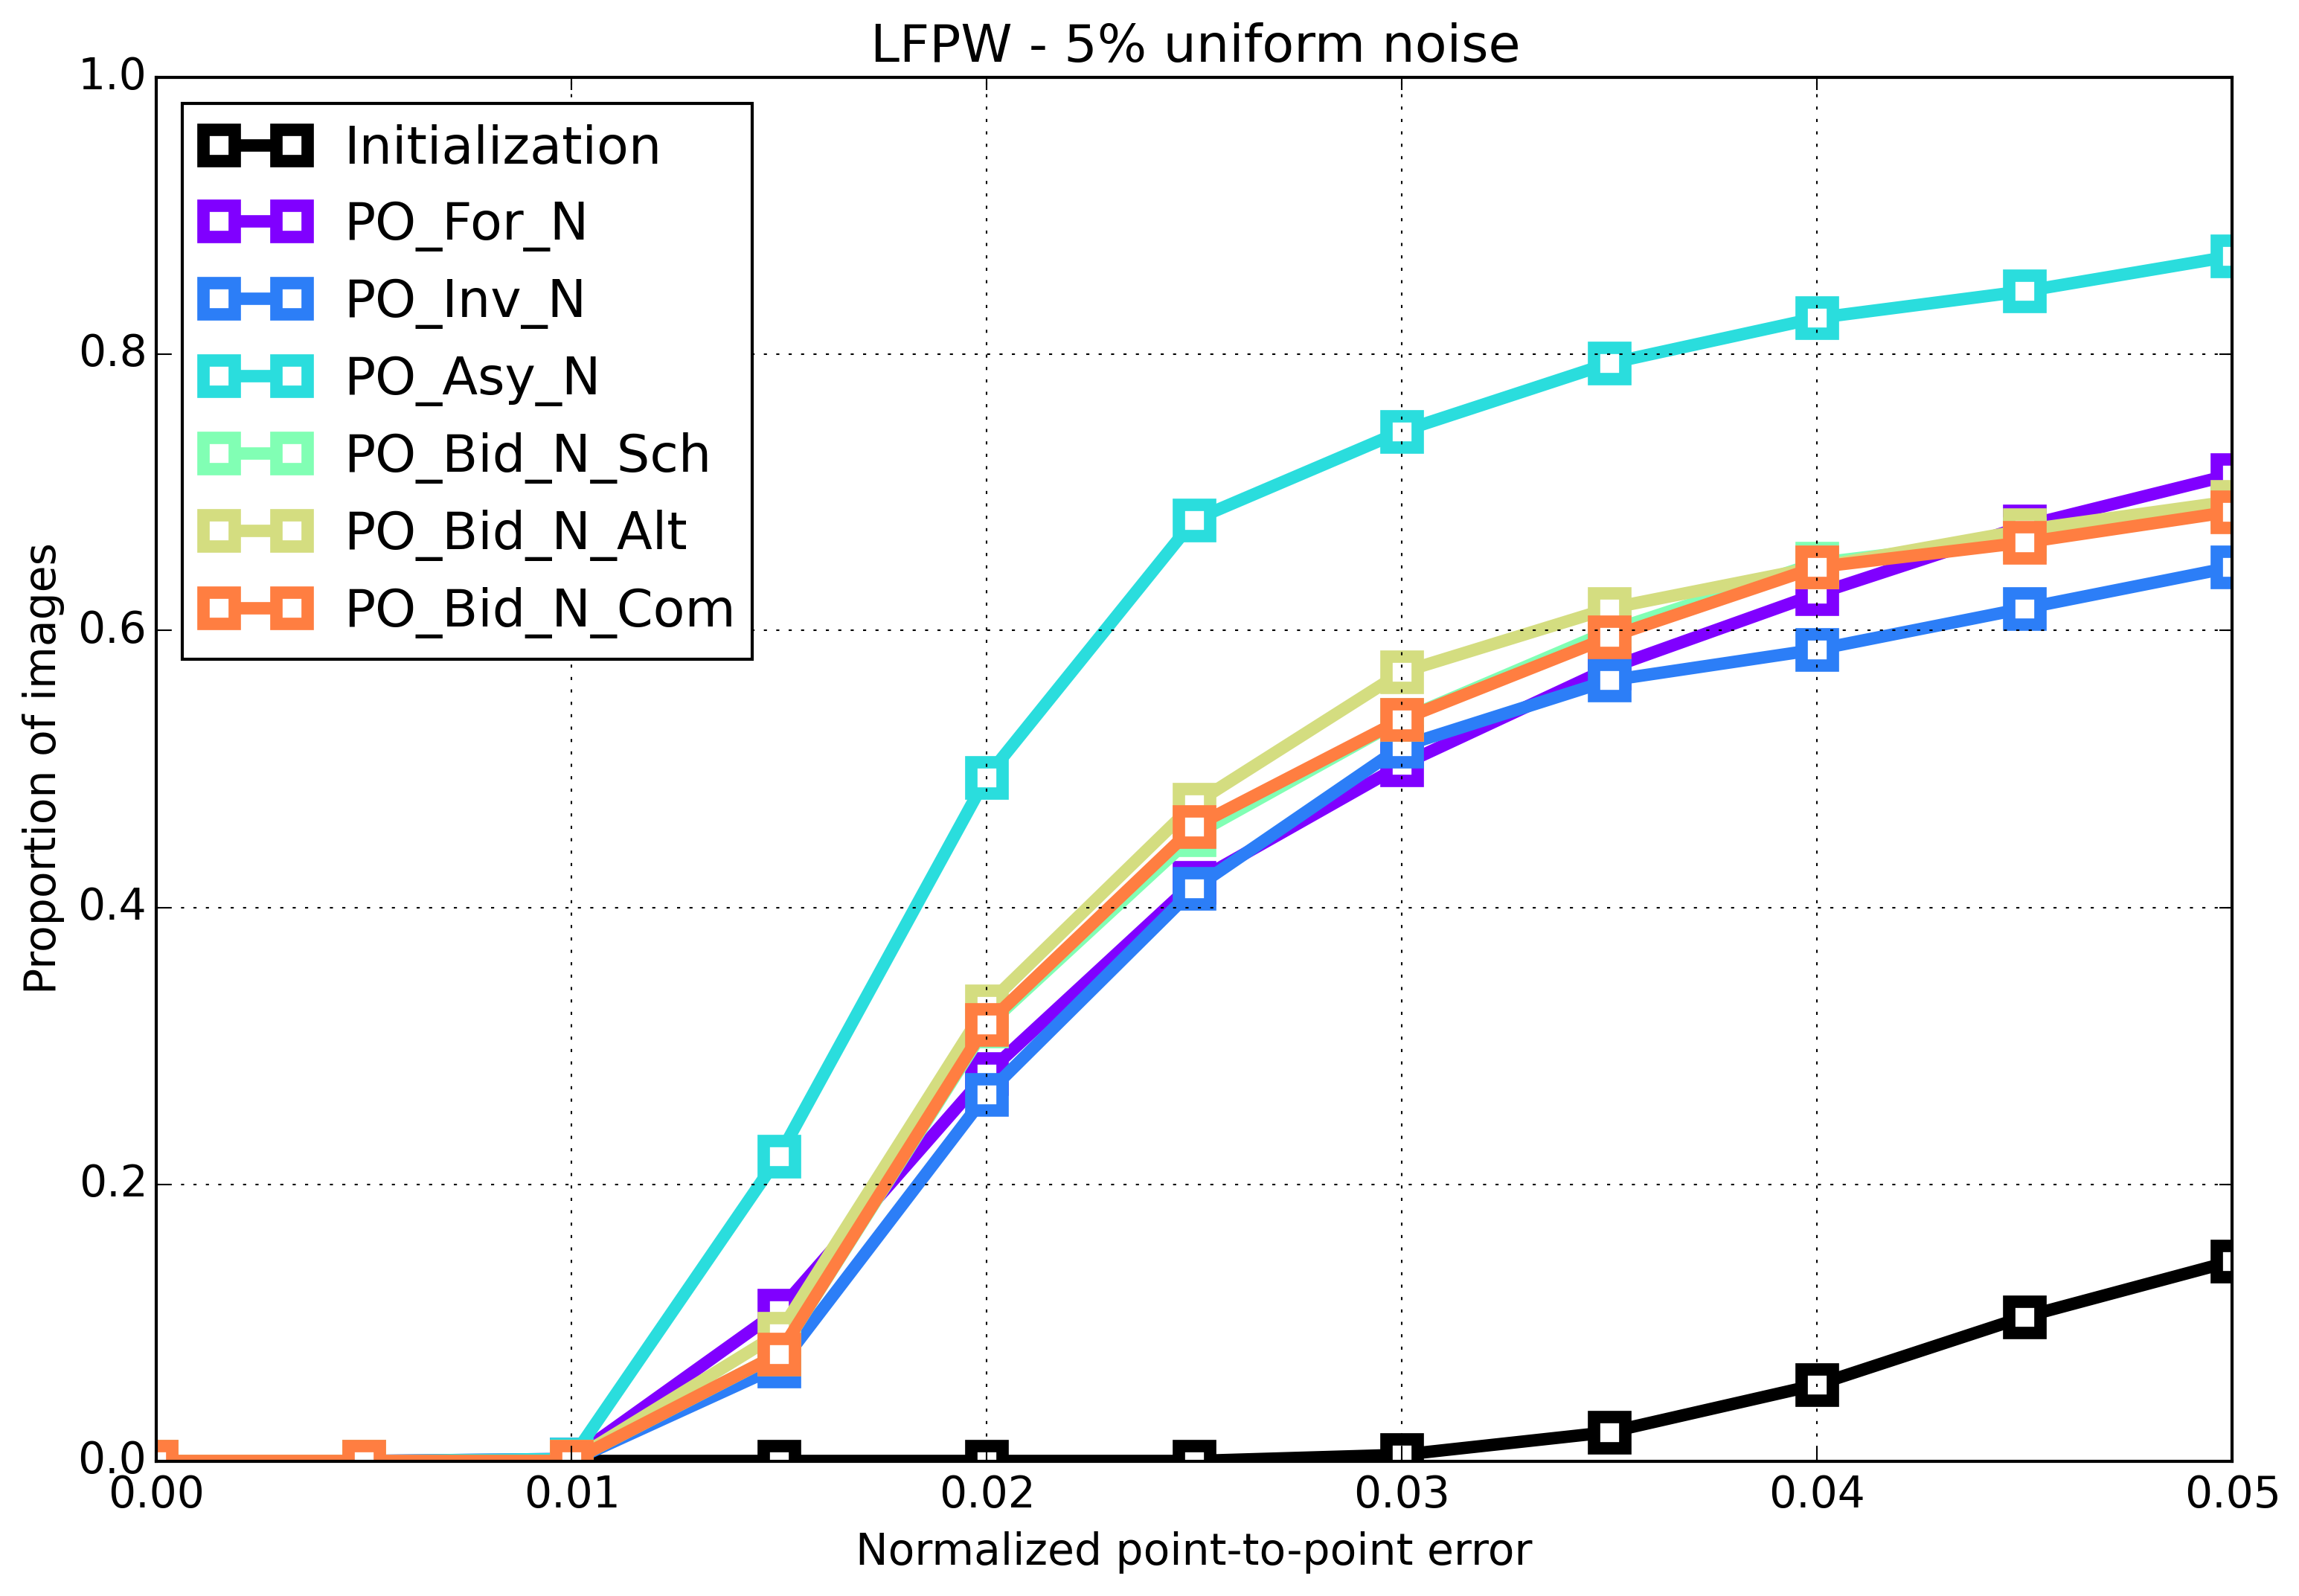
\includegraphics[width=\textwidth]{experiments/algorithms/po_n/ced_po_n_5.png}
	    \caption{CED graph on the LFPW test dataset for all Project-Out Newton algorithms initialized with $5\%$ uniform noise.}
	    \label{fig:ced_bpo_n_5}
	\end{subfigure}
	\hfill
	\begin{subfigure}{0.48\textwidth}
	    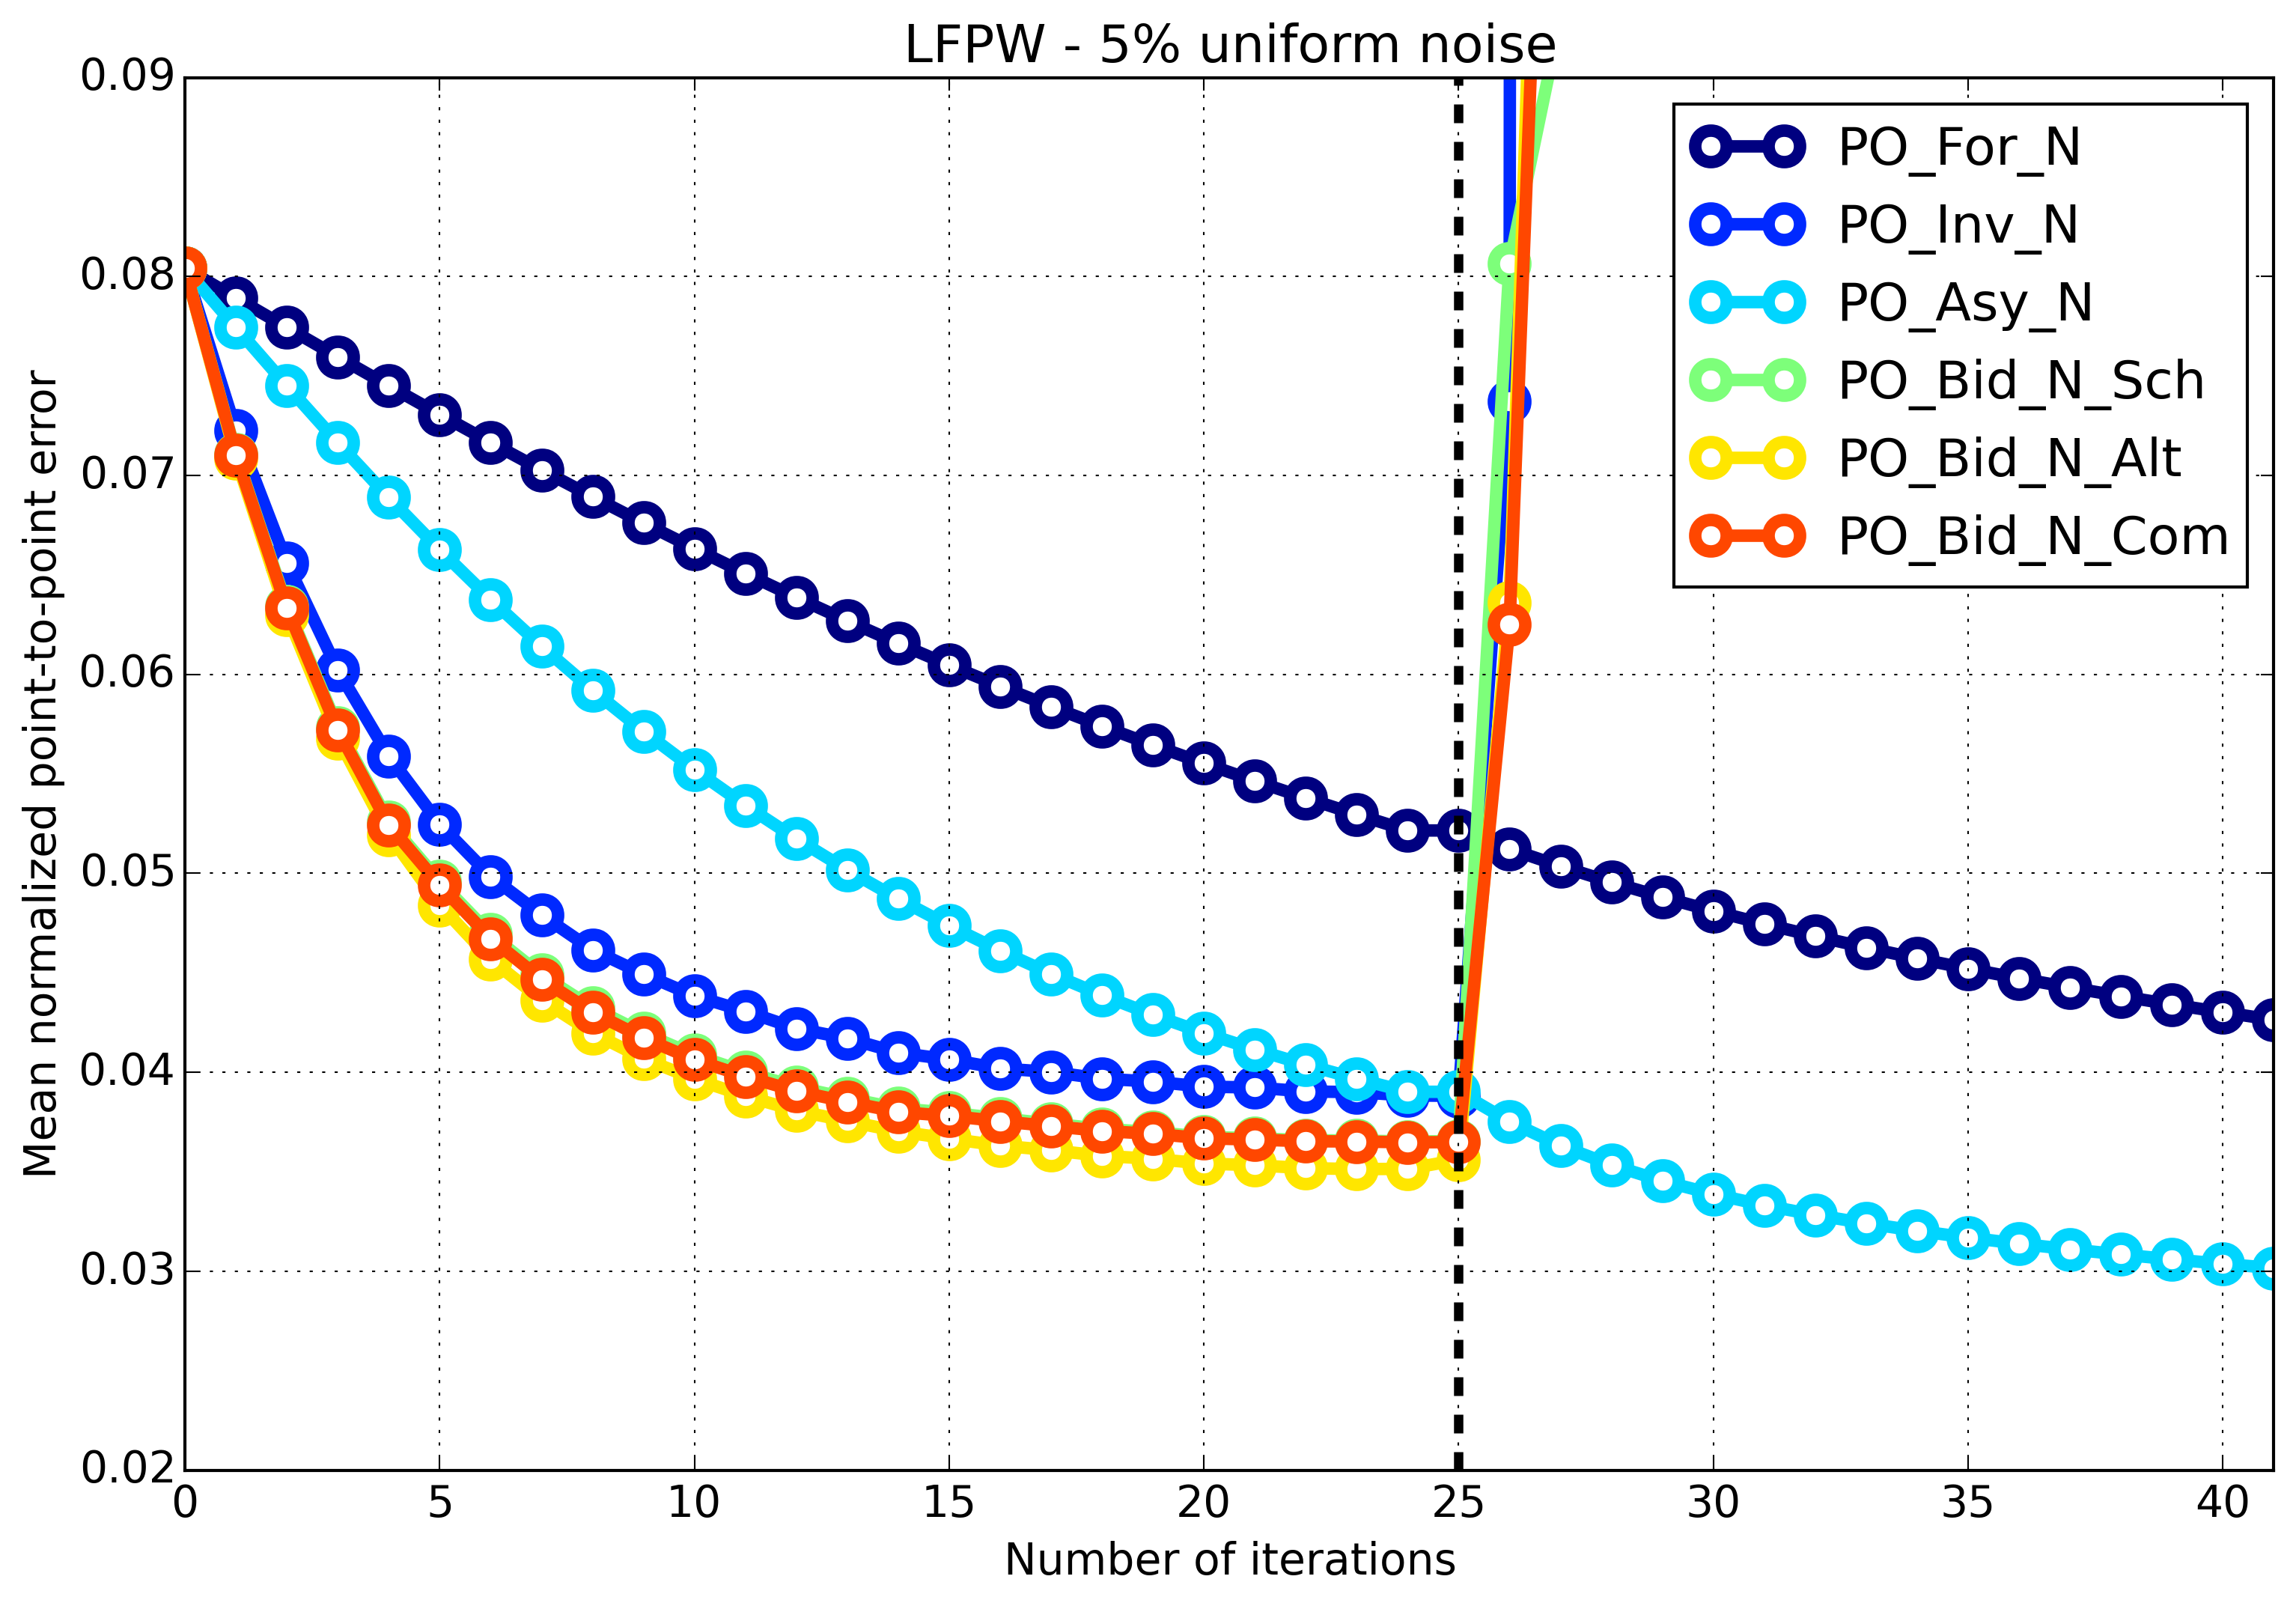
\includegraphics[width=\textwidth]{experiments/algorithms/po_n/mean_error_vs_iters_po_n_5.png}
	    \caption{Mean normalized point-to-point error vs number of iterations on the LFPW test dataset for all Project-Out Newton algorithms initialized with $5\%$ uniform noise.}
	    \label{fig:mean_error_vs_iters_bpo_n_5}
	\end{subfigure}
	\par\bigskip\bigskip
	\begin{subfigure}{0.48\textwidth}
	    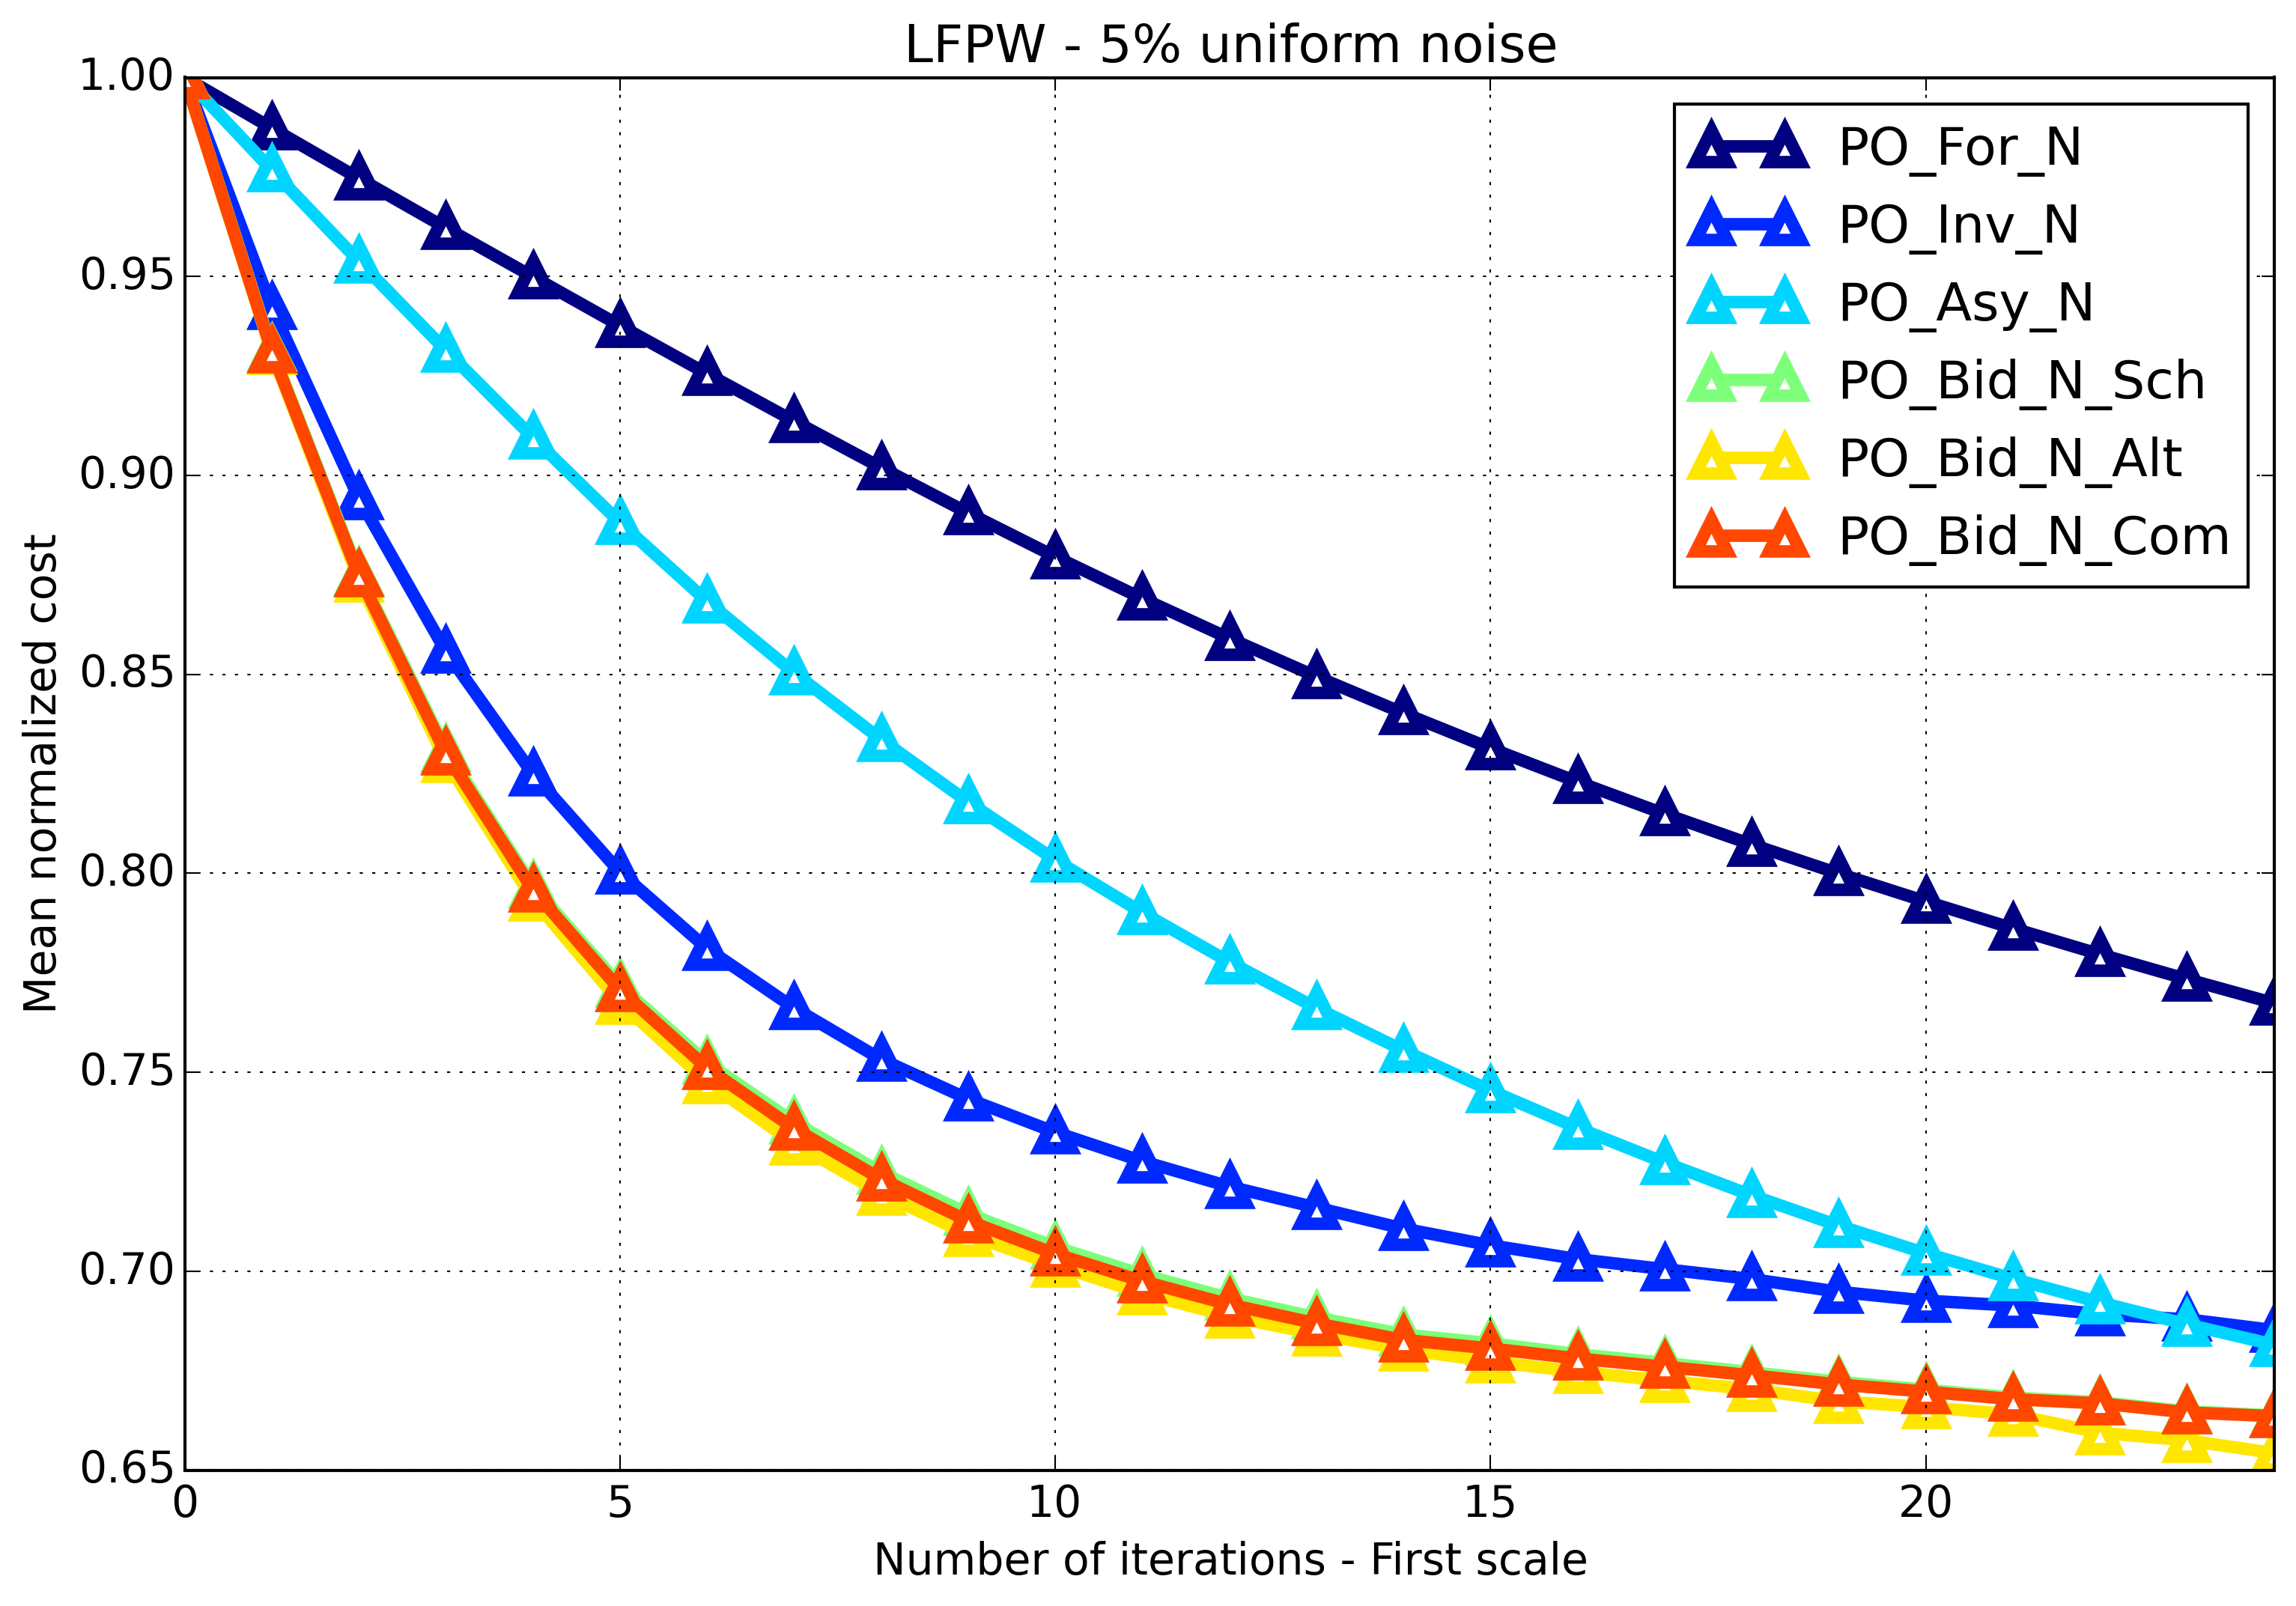
\includegraphics[width=\textwidth]{experiments/algorithms/po_n/mean_cost_vs_iters1_po_n_5.png}
	    \caption{Mean normalized cost vs number of first scale iterations on the LFPW test dataset for all Project-Out Newton algorithms initialized with $5\%$ uniform noise.}
	    \label{fig:mean_cost_vs_iters1_bpo_n_5}
	\end{subfigure}
	\hfill
	\begin{subfigure}{0.48\textwidth}
	    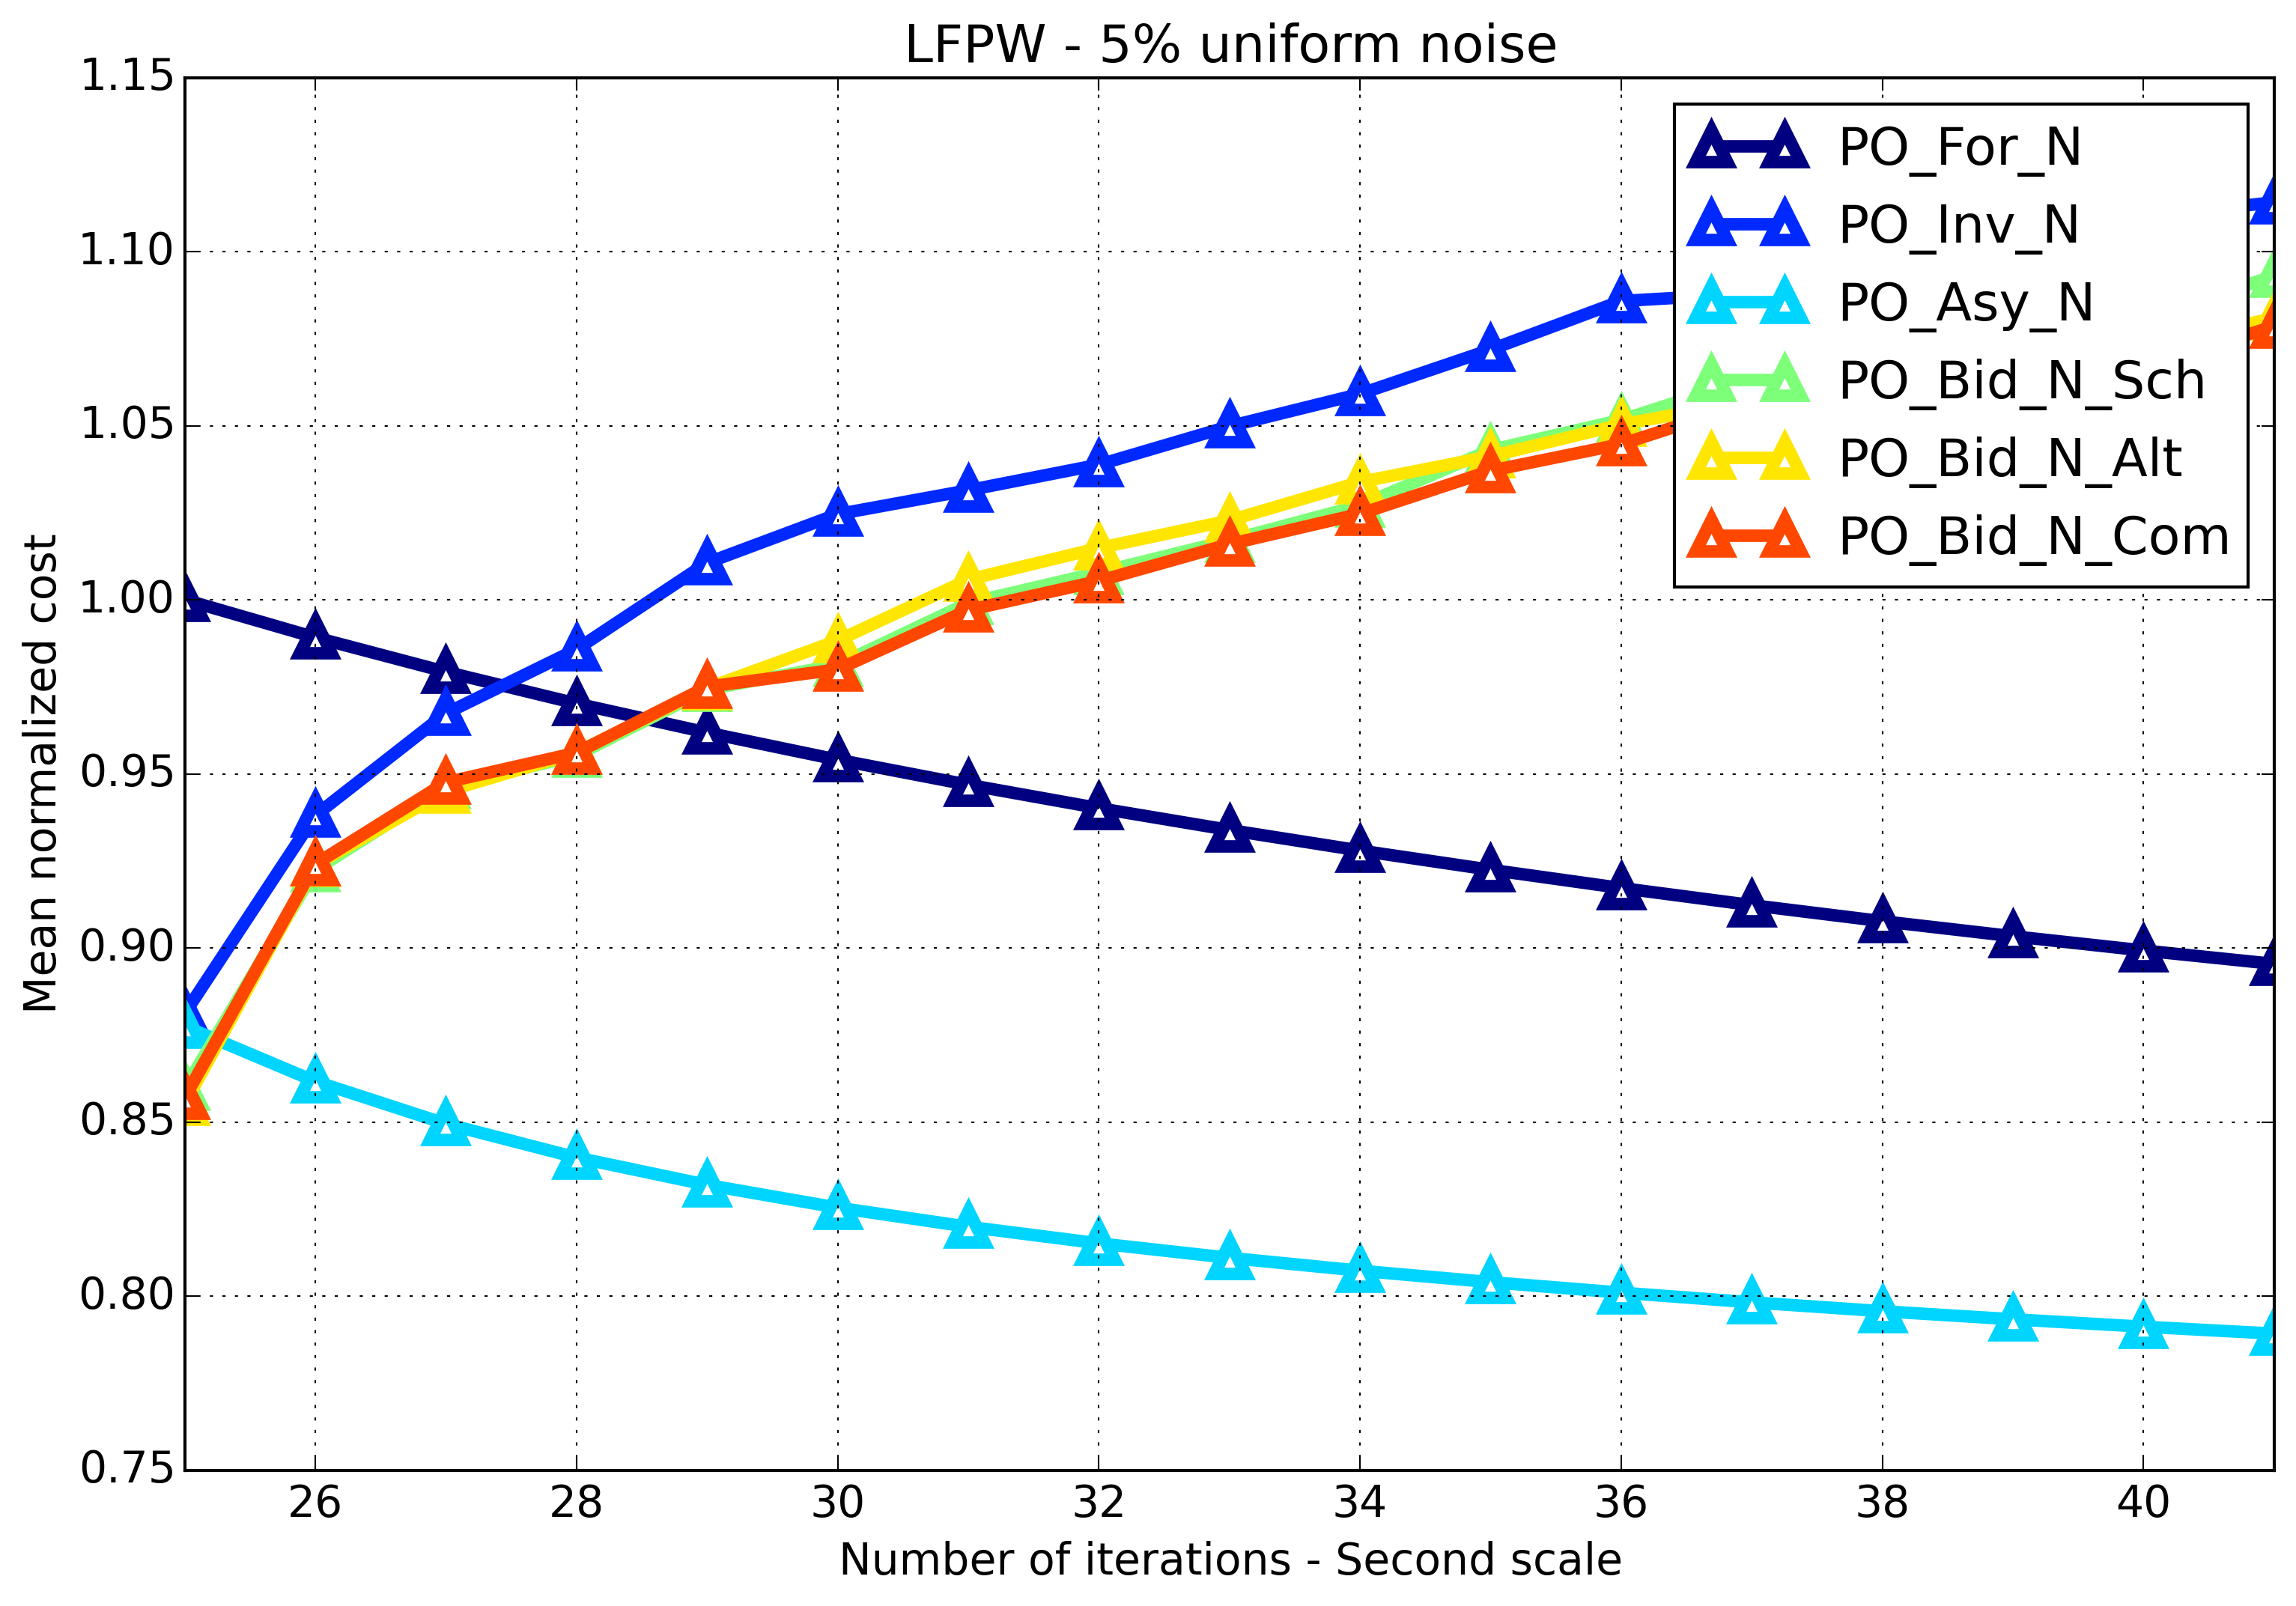
\includegraphics[width=\textwidth]{experiments/algorithms/po_n/mean_cost_vs_iters2_po_n_5.png}
	    \caption{Mean normalized cost vs number of second scale iterations on the LFPW test dataset for all Project-Out Newton algorithms initialized with $5\%$ uniform noise.}
	    \label{fig:mean_cost_vs_iters2_bpo_n_5}
	\end{subfigure}
	\par\bigskip\bigskip
	\begin{subfigure}{\textwidth}
		\center
		\begin{tabular}{lcccccc}
		    \toprule
		    Algorithm & $<0.02$ & $<0.03$ & $<0.04$ & Mean & Sdt & Median 
		    \\
		    \midrule
		    Initialization & 0.000 & 0.004 & 0.055 & 0.080 & 0.028 & 0.078
		    \\ 
		    PO\_For\_N\_Sch & 0.280 & 0.503 & 0.626 & 0.043 & 0.033 & 0.030
		    \\
		    PO\_Inv\_N\_Alt & 0.265 & 0.516 & 0.586 & 11.929 & 179.525 & 0.029
		    \\
		    PO\_Asy\_N\_Sch & \textbf{0.494} & \textbf{0.744} & \textbf{0.826} & \textbf{0.030} & \textbf{0.028} & \textbf{0.020}
		    \\
		    PO\_Bid\_N\_Sch & 0.314 & 0.536 & 0.649 & 0.287 & 1.347 & 0.027
		    \\
		    PO\_Bid\_N\_Alt & 0.329 & 0.570 & 0.649 & 0.280 & 1.465 & 0.026
		    \\
		    \bottomrule
	  	\end{tabular}
	  	\caption{Table showing the proportion of images fitted with a normalized point-to-point error below $0.02$, $0.03$ and $0.04$ together with the normalized point-to-point error Mean, Std and Median for all Project-Out Newton algorithms initialized with $5\%$ uniform noise.}
	    \label{tab:stats_bpo_n_5}
	\end{subfigure}
	\caption{Results showing the fitting accuracy and convergence properties of the Project-Out Newton algorithms on the LFPW test dataset.}
	\label{fig:bpo_n_5}
\end{figure*}


\begin{figure*}[p]
	\centering
	\begin{subfigure}{0.48\textwidth}
	    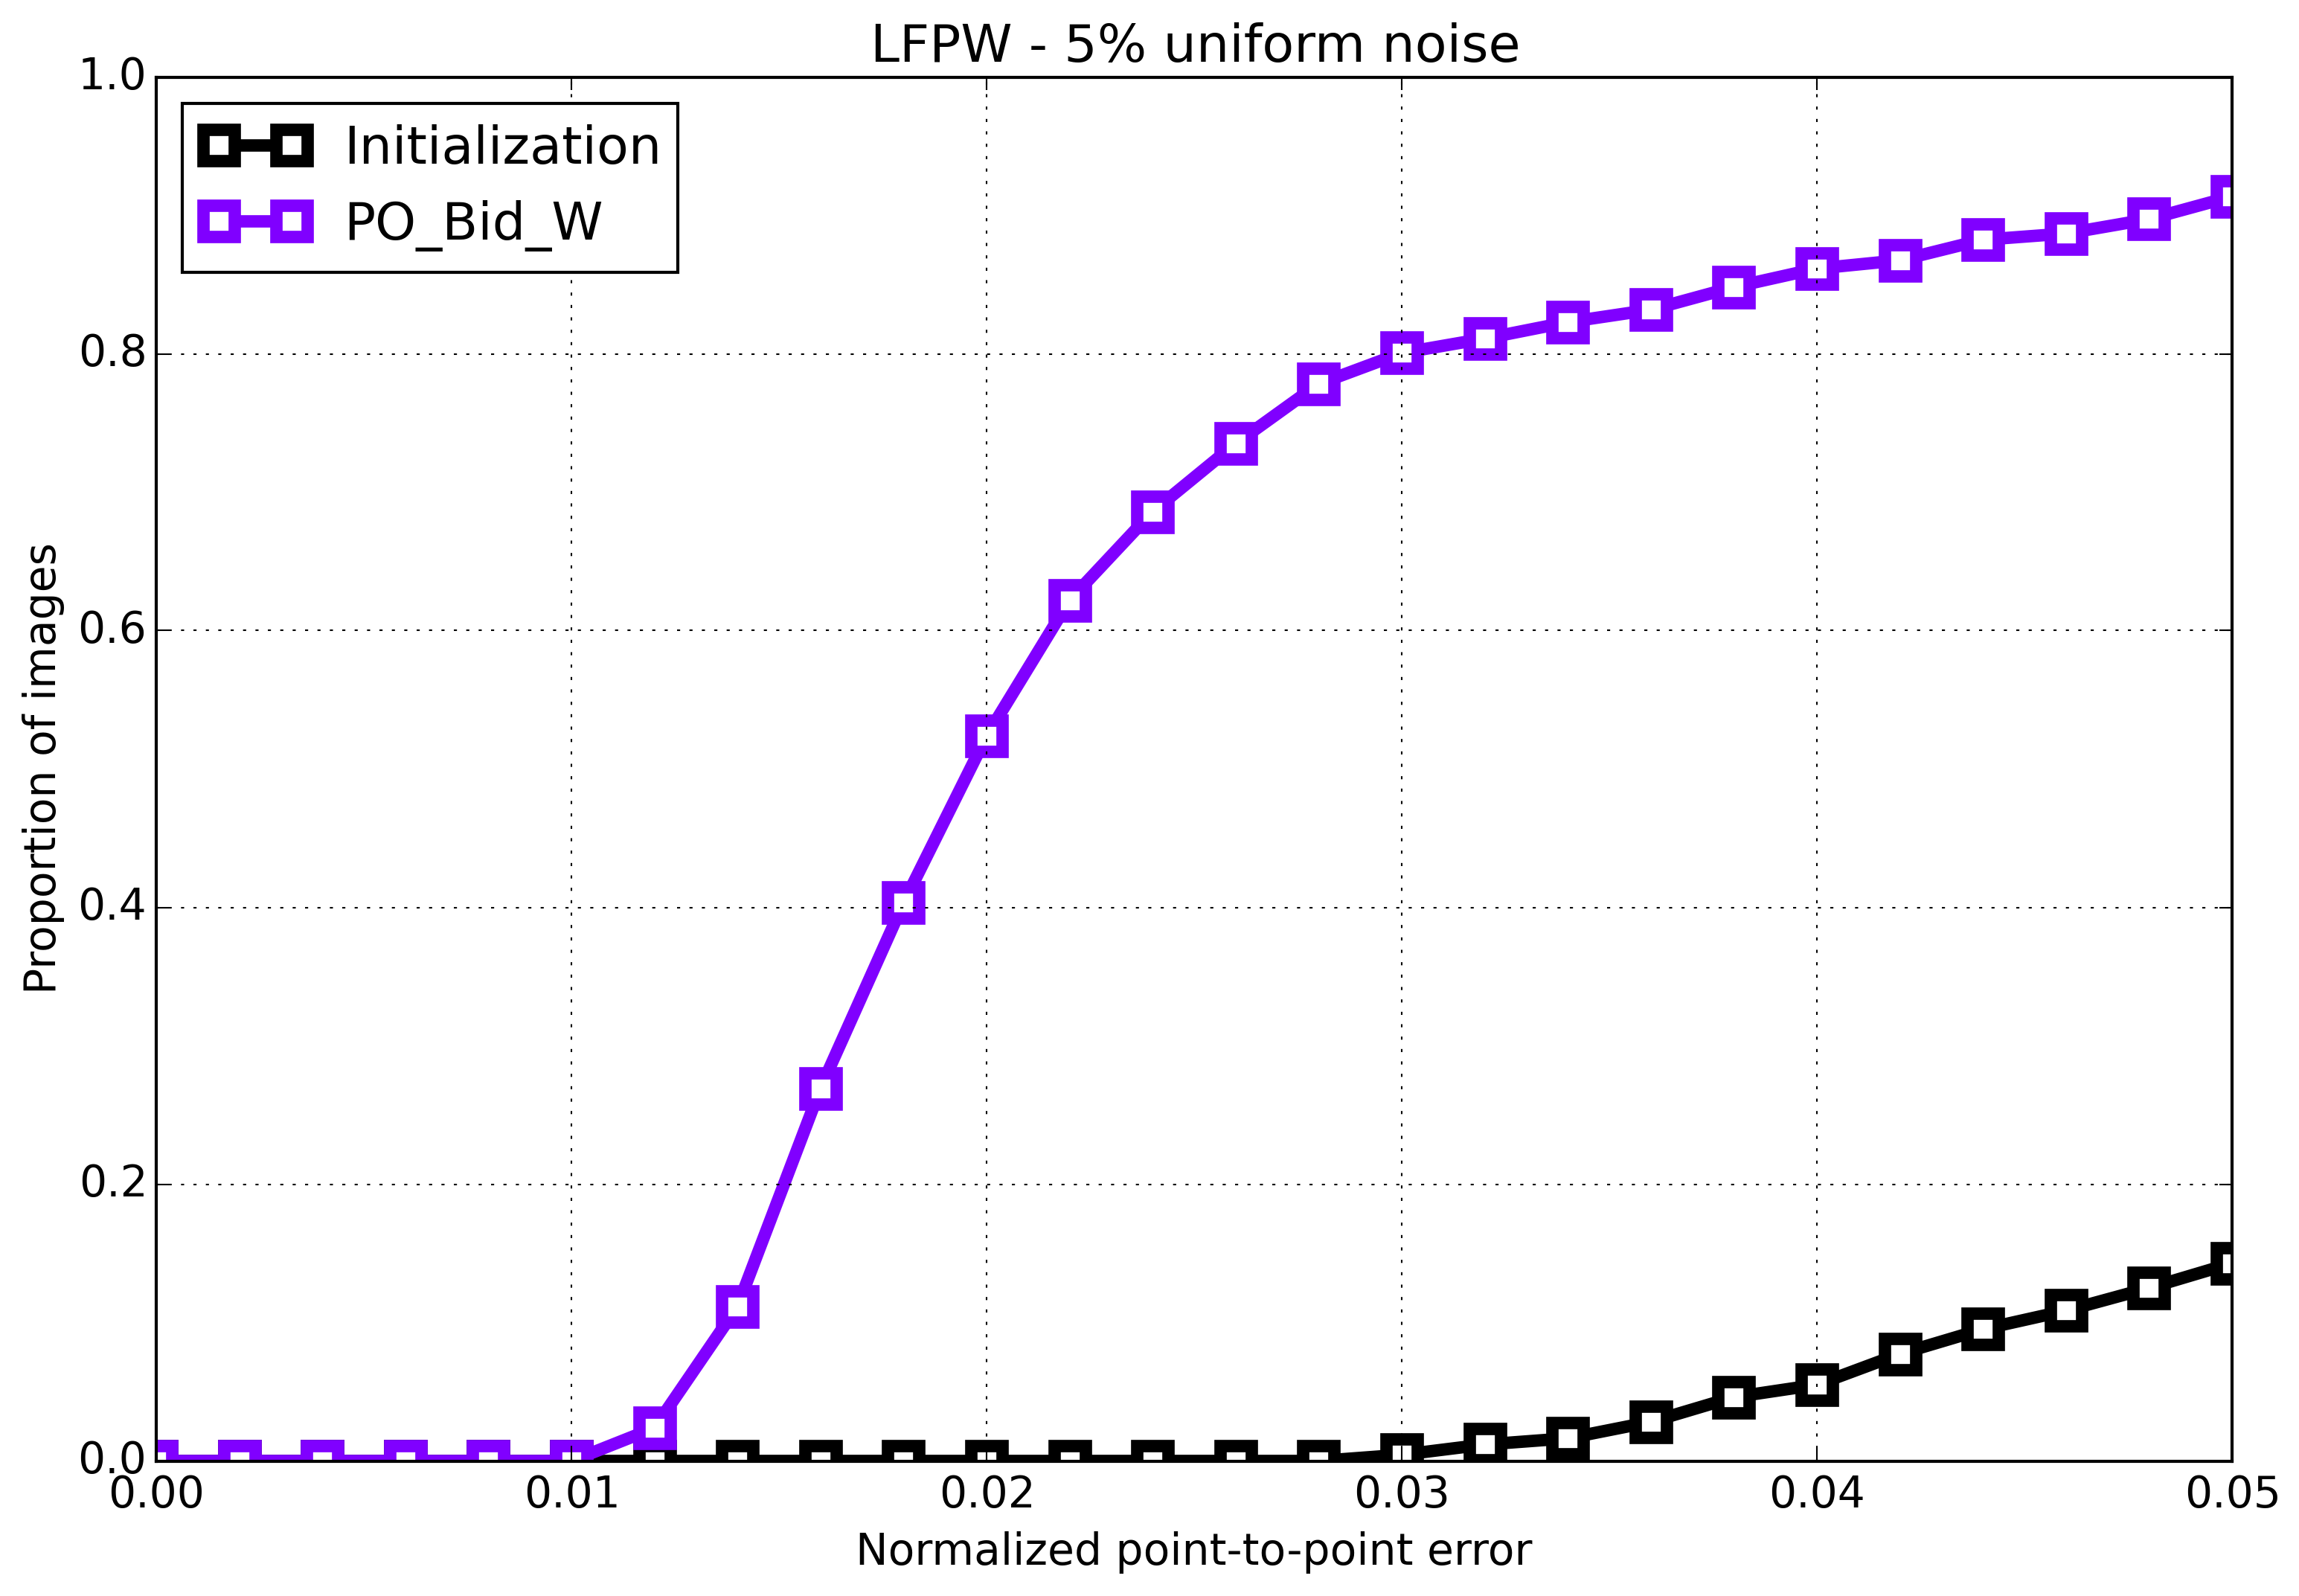
\includegraphics[width=\textwidth]{experiments/algorithms/po_w/ced_po_w_5.png}
	    \caption{Cumulative Error Distribution graph on the LFPW test dataset for all Project-Out Wiberg algorithms initialized with $5\%$ uniform noise.}
	    \label{fig:ced_bpo_w_5}
	\end{subfigure}
	\hfill
	\begin{subfigure}{0.48\textwidth}
	    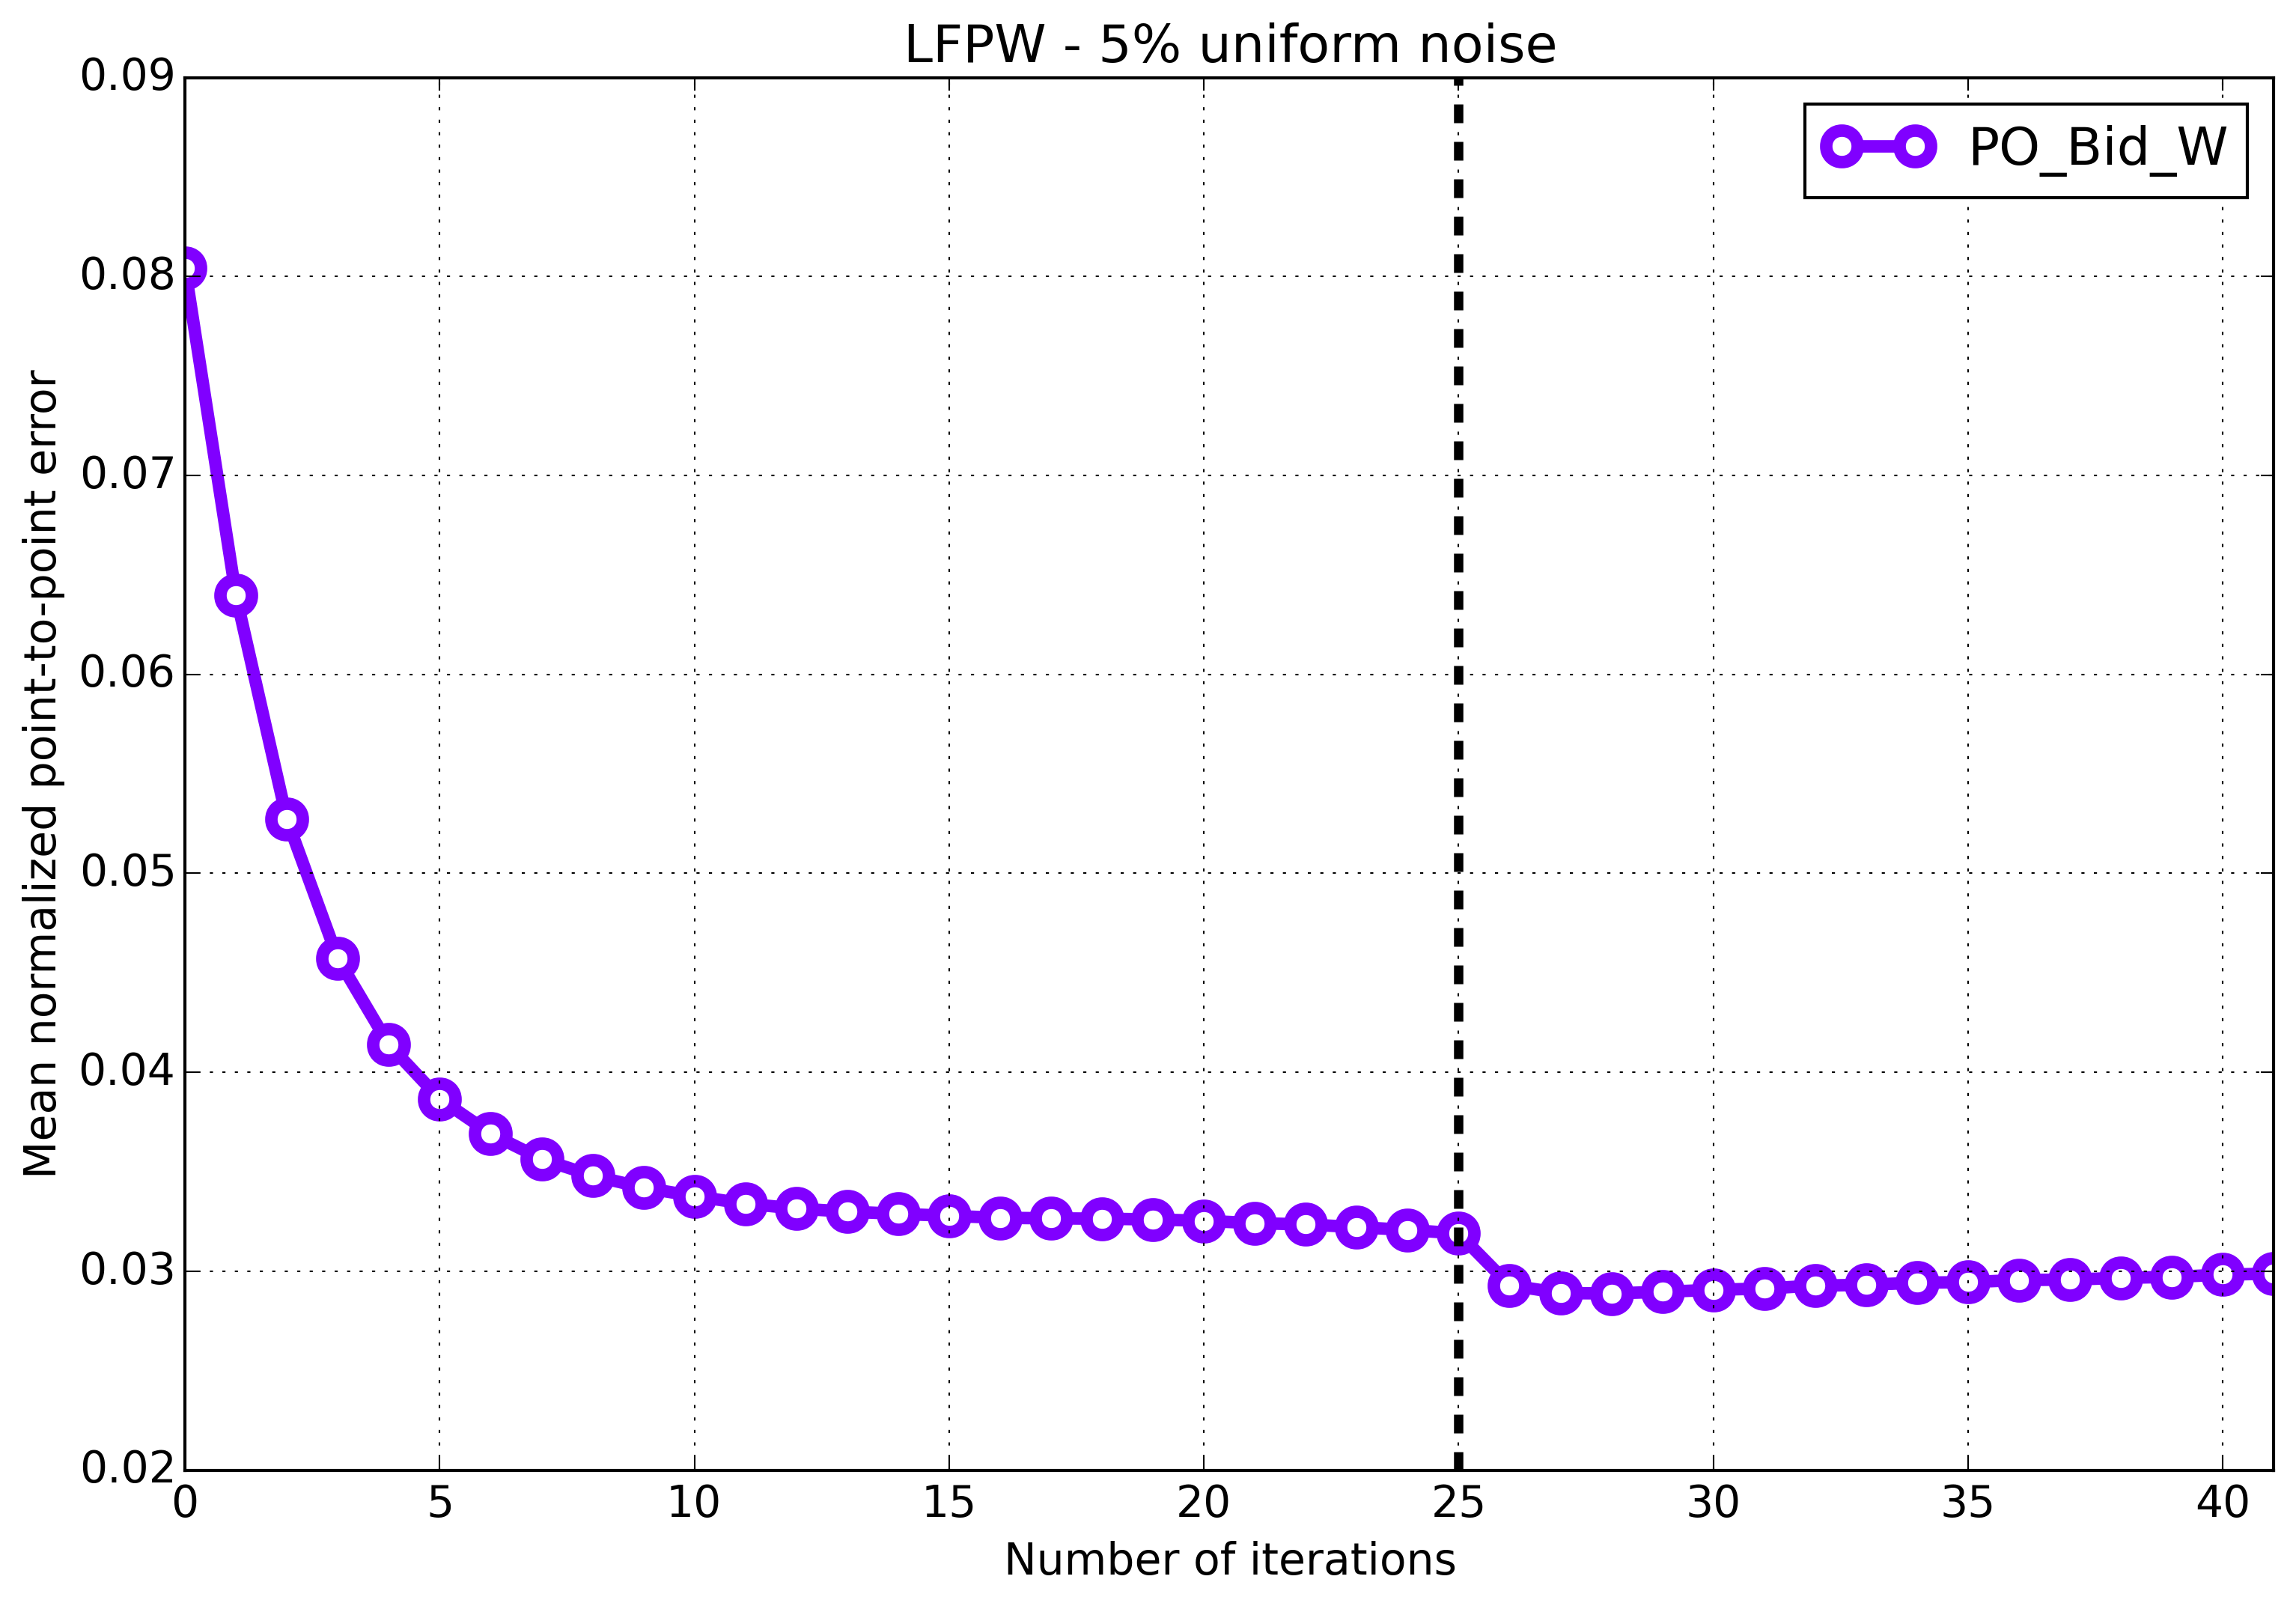
\includegraphics[width=\textwidth]{experiments/algorithms/po_w/mean_error_vs_iters_po_w_5.png}
	    \caption{Mean normalized point-to-point error vs number of iterations graph on the LFPW test dataset for all Project-Out Wiberg algorithms initialized with $5\%$ uniform noise.}
	    \label{fig:mean_error_vs_iters_bpo_w_5}
	\end{subfigure}
	\par\bigskip\bigskip
	\begin{subfigure}{0.48\textwidth}
	    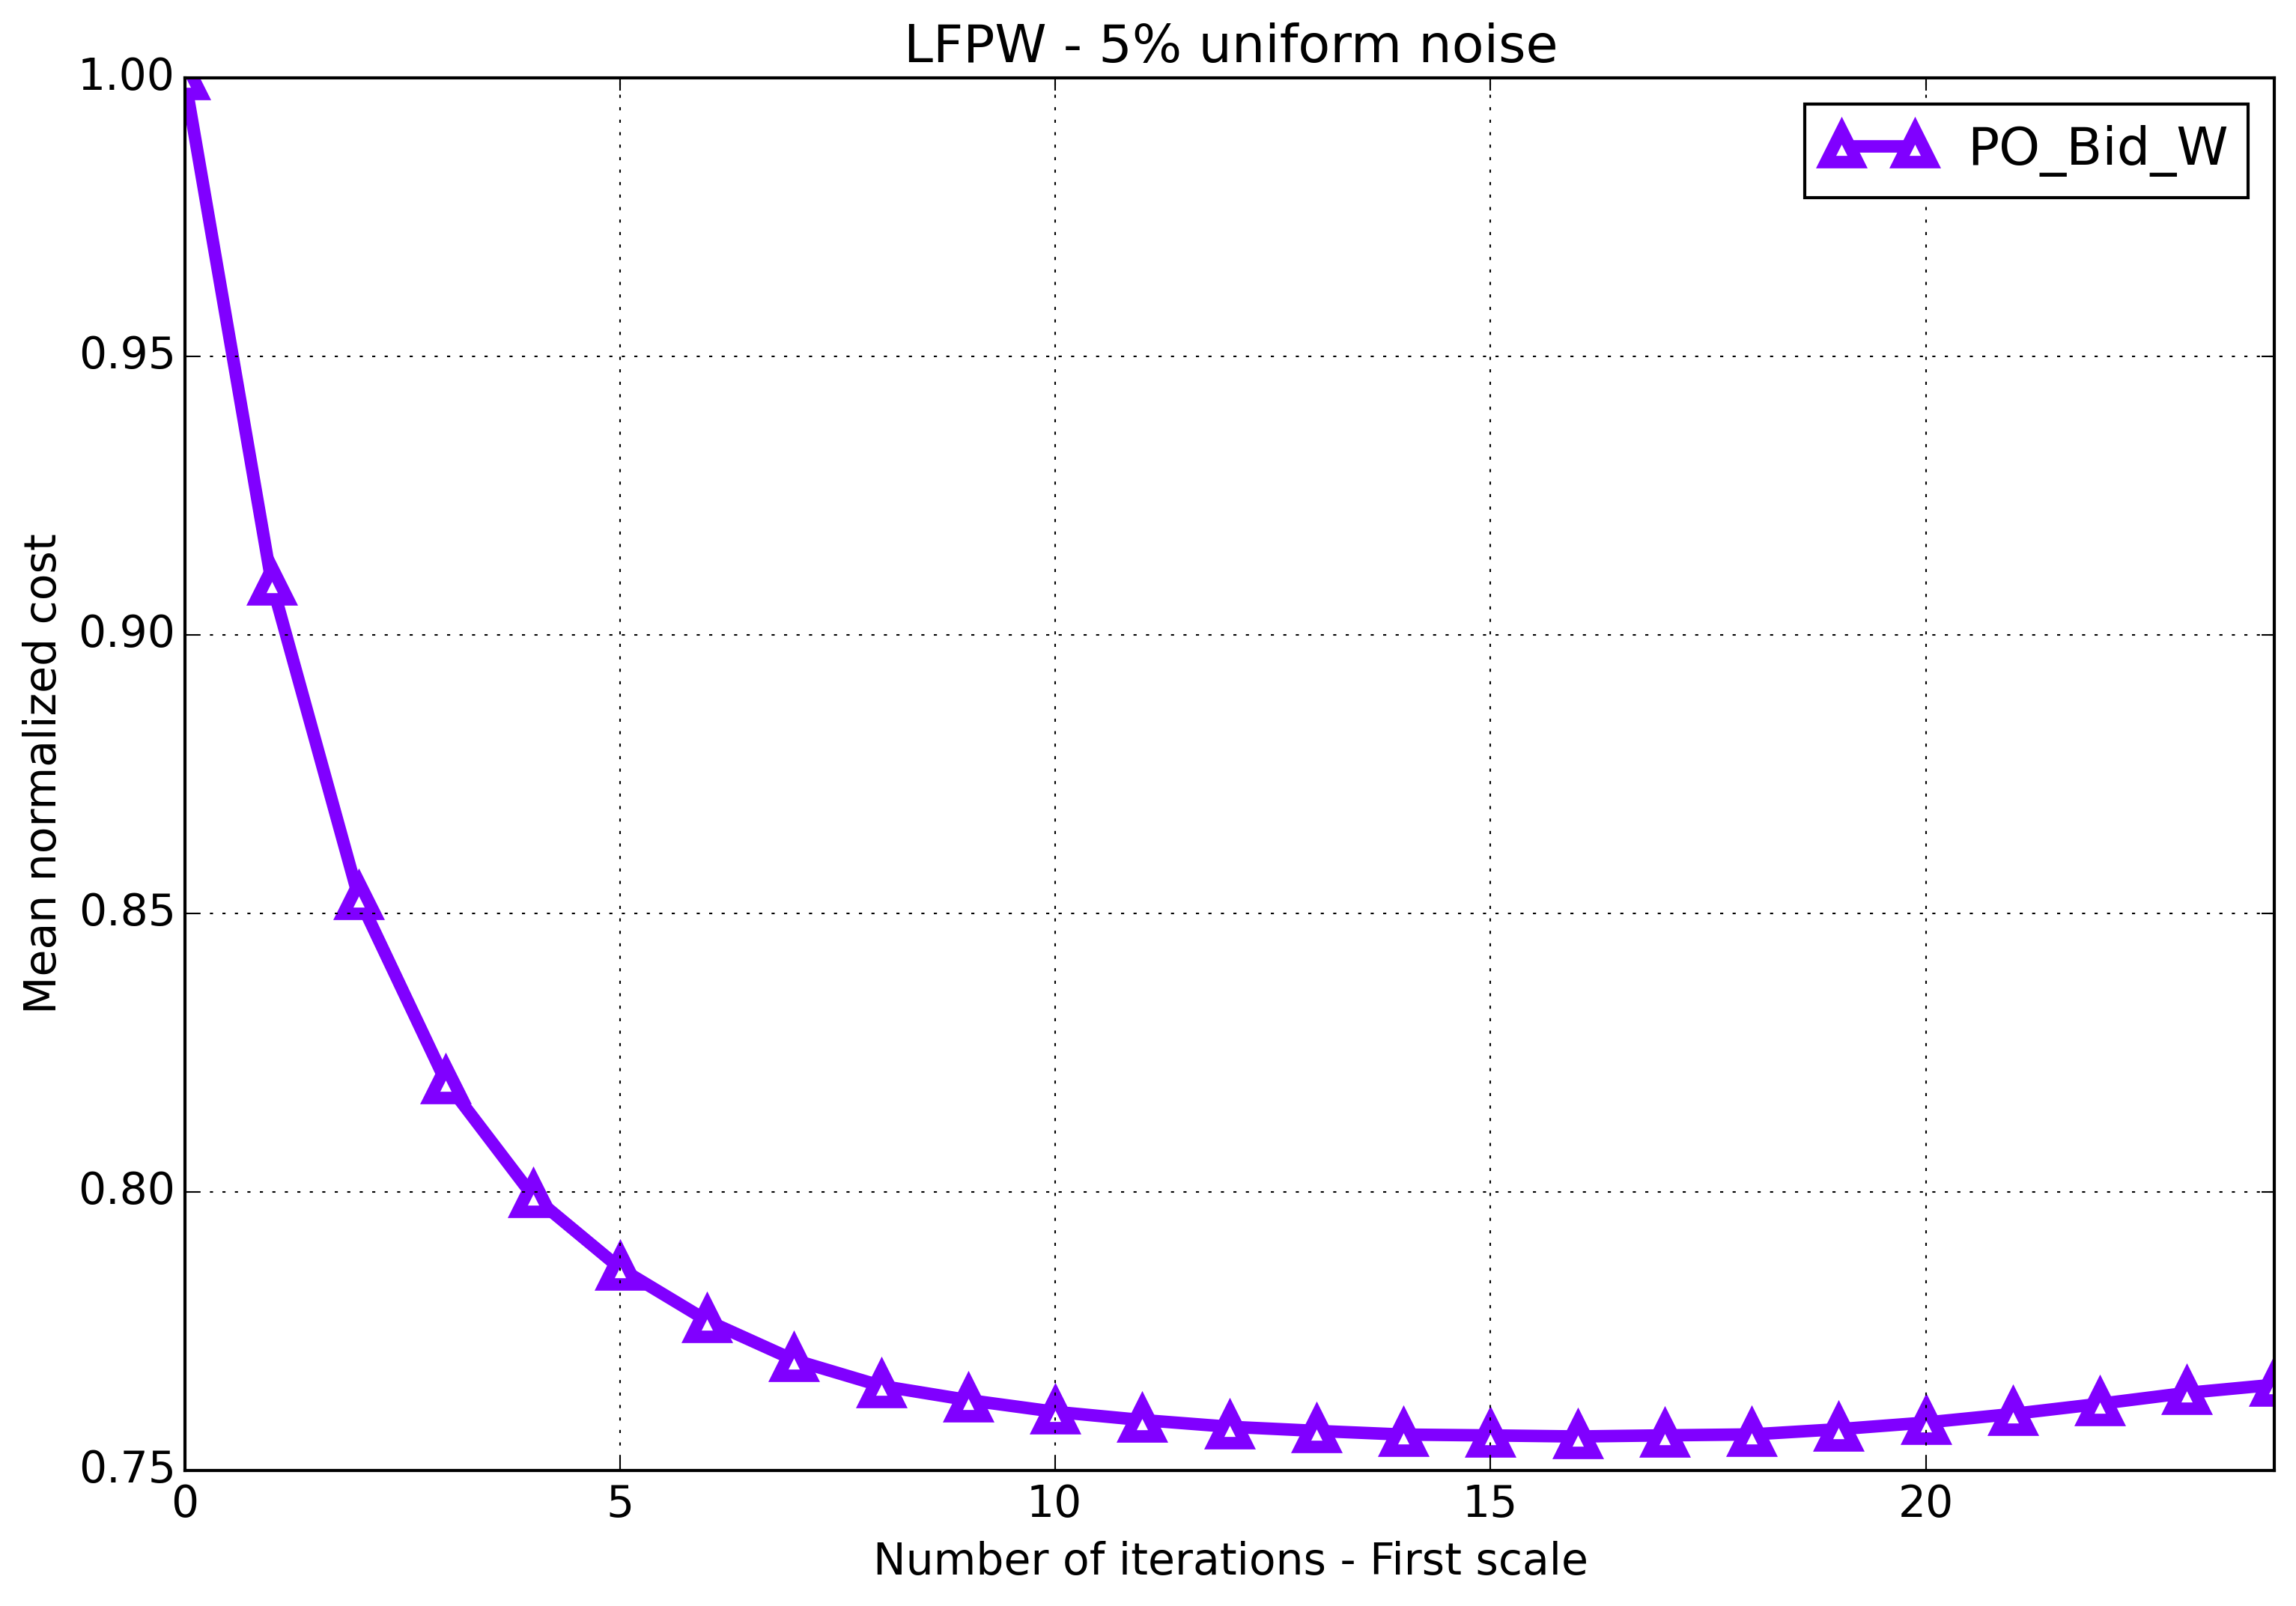
\includegraphics[width=\textwidth]{experiments/algorithms/po_w/mean_cost_vs_iters1_po_w_5.png}
	    \caption{Mean normalized cost vs number of first scale iterations graph on the LFPW test dataset for all Project-Out Wiberg algorithms initialized with $5\%$ uniform noise.}
	    \label{fig:mean_cost_vs_iters1_bpo_w_5}
	\end{subfigure}
	\hfill
	\begin{subfigure}{0.48\textwidth}
	    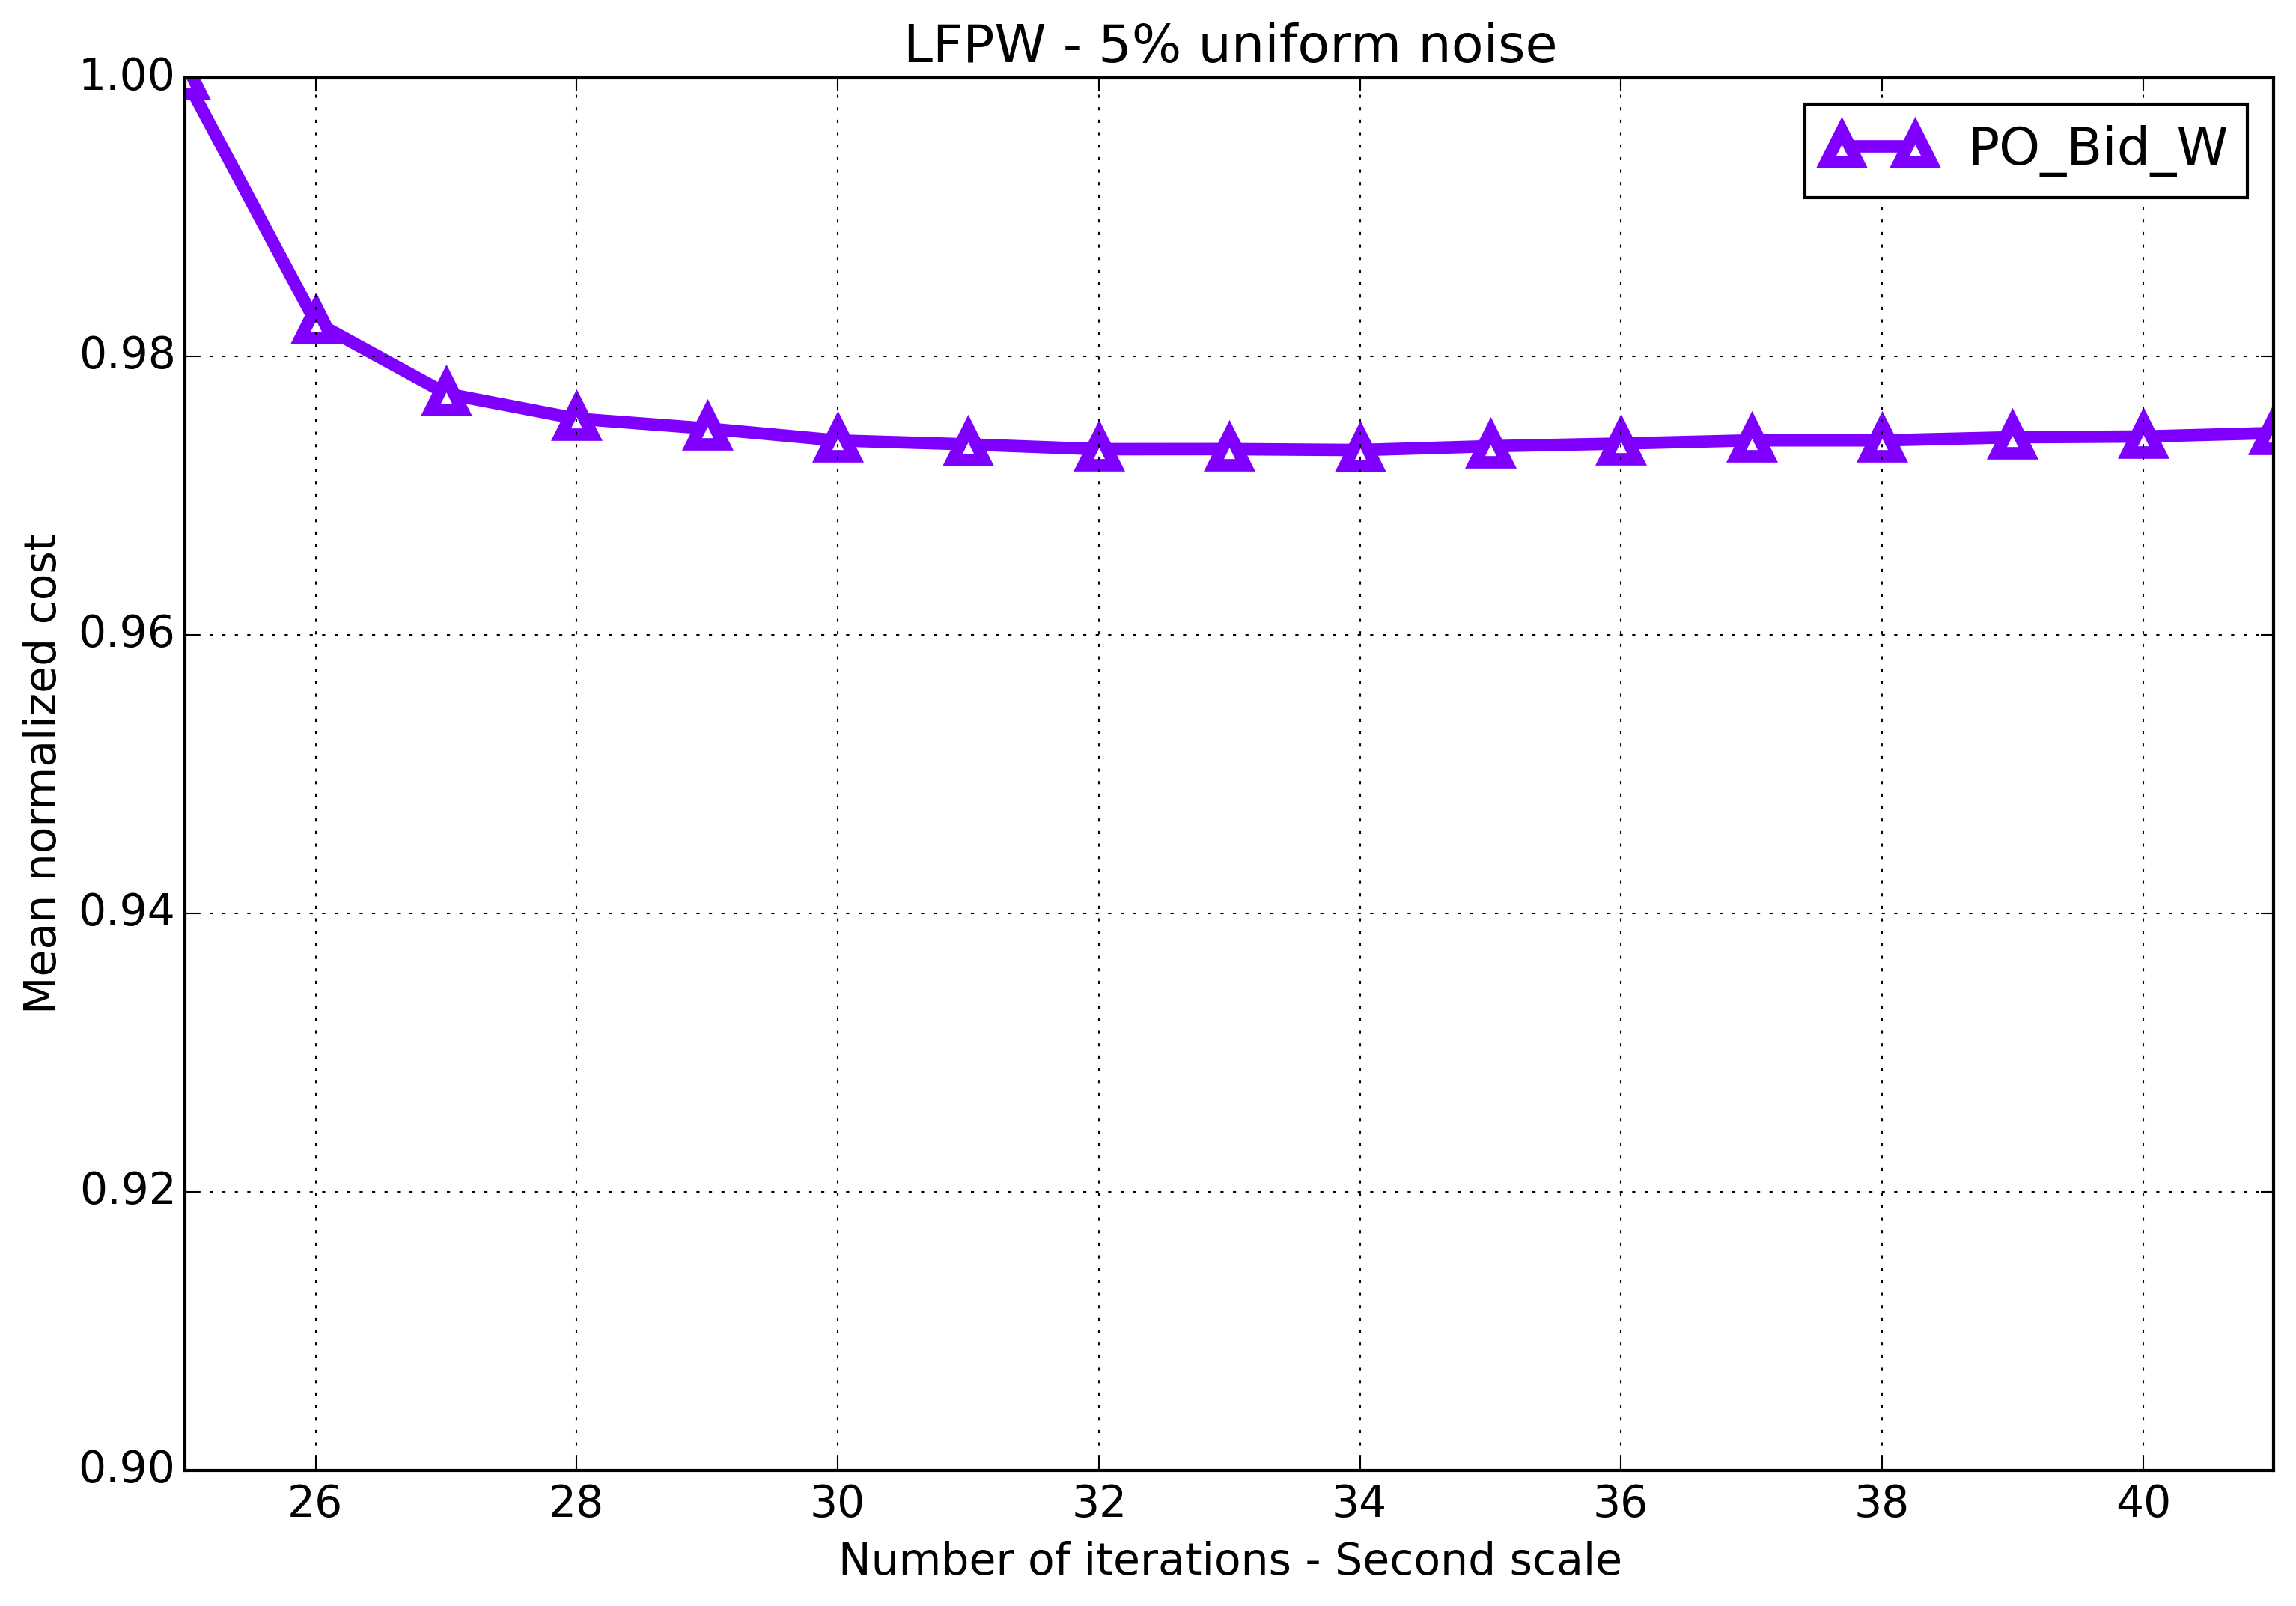
\includegraphics[width=\textwidth]{experiments/algorithms/po_w/mean_cost_vs_iters2_po_w_5.png}
	    \caption{Mean normalized cost vs number of second scale iterations graph on the LFPW test dataset for all Project-Out Wiberg algorithms initialized with $5\%$ uniform noise.}
	    \label{fig:mean_cost_vs_iters2_bpo_w_5}
	\end{subfigure}
	\par\bigskip\bigskip
	\begin{subfigure}{\textwidth}
		\center
		\begin{tabular}{lcccccc}
		    \toprule
		    Algorithm & $<0.02$ & $<0.03$ & $<0.04$ & Mean & Sdt & Median 
		    \\
		    \midrule
		    Initialization & 0.000 & 0.004 & 0.055 & 0.080 & 0.028 & 0.078
		    \\ 
		    PO\_Bid\_W\_Sch & 0.524 & 0.801 & 0.862 & 0.030 & 0.039 & 0.020
		    \\
		    \bottomrule
	  	\end{tabular}
	  	\caption{Table showing the proportion of images fitted with a normalized point-to-point error below $0.02$, $0.03$ and $0.04$ together with the normalized point-to-point error Mean, Std and Median for all Project-Out Wiberg algorithms initialized with $5\%$ uniform noise.}
	    \label{tab:stats_bpo_w_5}
	\end{subfigure}
	\caption{Results showing the fitting accuracy and convergence properties of the Project-Out Wiberg algorithms on the LFPW test dataset.}
	\label{fig:bpo_w_5}
\end{figure*}


% \begin{figure}[h!]
%     \centering
%     \includegraphics[width=0.50\textwidth]{experiments/algorithms/ssd_gn/ced_ssd_gn_4.png}
%     \caption{CED graph on the LFPW test dataset for all SSD Gauss-Newton algorithms initialized with $4$\% of uniform noise.}
%     \label{fig:ced_po_asymmetric_gn_4}
% \end{figure}




% \begin{figure}[h!]
%     \centering
%     \includegraphics[width=0.50\textwidth]{experiments/algorithms/ssd_gn/mean_error_vs_iters_ssd_gn_4.png}
%     \caption{Mean normalized point-to-point error vs number of iterations graph on the LFPW test dataset for all SSD Gauss-Newton algorithms initialized with $4$\% of uniform noise}
%     \label{fig:mean_error_vs_iters_po_asymmetric_gn_4}
% \end{figure}


\subsection{Weighted Bayesian project-out}

In this experiment, we quantify the importance of each of the two terms in our Bayesian project-out cost function, Equation \ref{eq:prob_po}. To this end, we introduce the parameters, $\rho \in [0, 1]$ and $\gamma = 1 - \rho$, to weight up the relative contribution of both terms as follows:
\begin{equation}
    \begin{aligned}
        \rho|| \mathbf{i}[\mathbf{p}] - \mathbf{\bar{a}} ||^2_{\mathbf{A}\mathbf{D}^{-1}\mathbf{A}^T} 
        + 
        \frac{\gamma}{\sigma^2}|| \mathbf{i}[\mathbf{p}] - \mathbf{\bar{a}} ||^2_{\bar{\mathbf{A}}}
    \end{aligned}
    \label{eq:weighted_po}
\end{equation}
Setting $\rho=0$, $\gamma=1$ reduces the previous cost function to the original project-out loss proposed in \cite{Matthews2004}; completely disregarding the contribution of the prior distribution over the appearance parameters i.e the Mahalanobis distance \emph{within} the appearance subspace. On the contrary, setting $\rho=1$, $\gamma=0$ reduces the cost function to the first term; completely disregarding the contribution of the project-out term i.e. the distance \emph{to} the appearance subspace. Finally setting $\rho=\gamma=0.5$ leads to the standard Bayesian project-out cost function proposed in Section \ref{sec:po_pi}.
 
In order to asses the impact that each term has on the fitting accuracy obtained by the previous project-out algorithm we repeat the experimental set up of the first experiment and test all project-out algorithms for different values of the parameters $\rho$ and $\gamma$. Results for this experiment are reported by Figure \ref{fig:rho}. We can see that, regardless of the type of composition, a weighted combinations of the two previous terms always leads to a smaller mean normalized point-to-point error compared to either term on its own. Note that the accuracy achieved by the standard Bayesian project-out cost function is substantially better than the one obtained by the original project-out loss (specially noticeable for the inverse and bidirectional cases); fully justifying the inclusion of the first term, i.e the Mahalanobis distance \emph{within} the appearance subspace, into the cost function. Finally, in this particular experiment, the accuracy of all algorithms is maximized by setting $\rho=0.1$, $\gamma=0.9$, further highlighting the importance of the first term in the Bayesian formulation.

\begin{figure*}[p]
	\centering
	\begin{subfigure}{\textwidth}
	    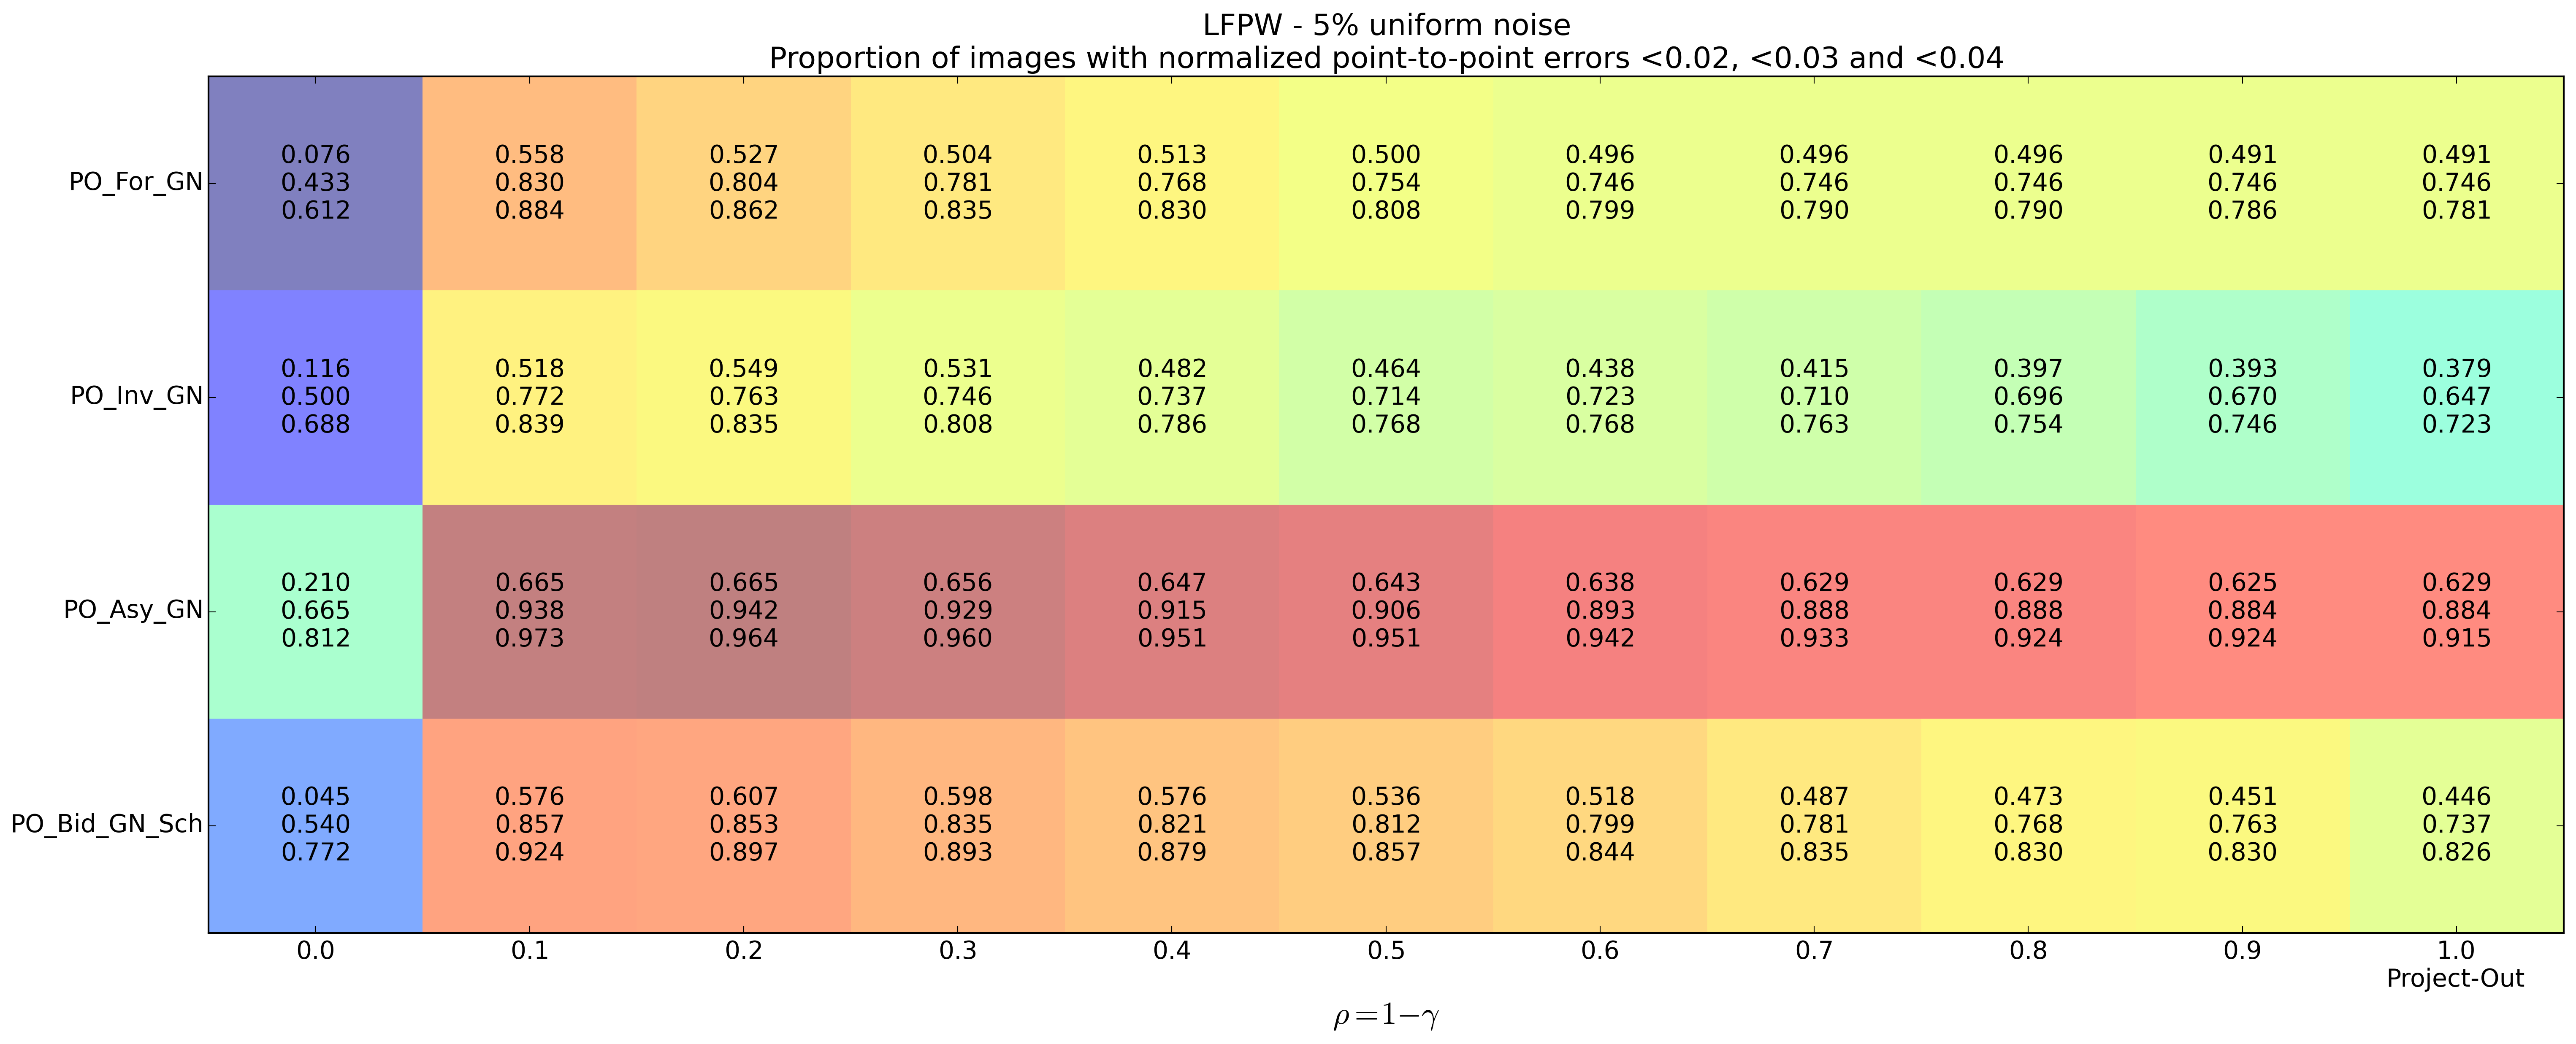
\includegraphics[width=\textwidth]{experiments/rho/convergence_vs_rho_po_gn_5.png}
	    \caption{Proportion of images with normalized point-to-point errors smaller than $0.02$, $0.03$ and $0.04$ for the Project-Out and SSD Asymmetric Gauss-Newton algorithms values of $\rho$ and $\gamma$ and initialized with $5\%$ noise.}
	    \label{fig:convergence_vs_rho_po_gn}
	\end{subfigure}
	\par\bigskip
	\begin{subfigure}{0.48\textwidth}
	    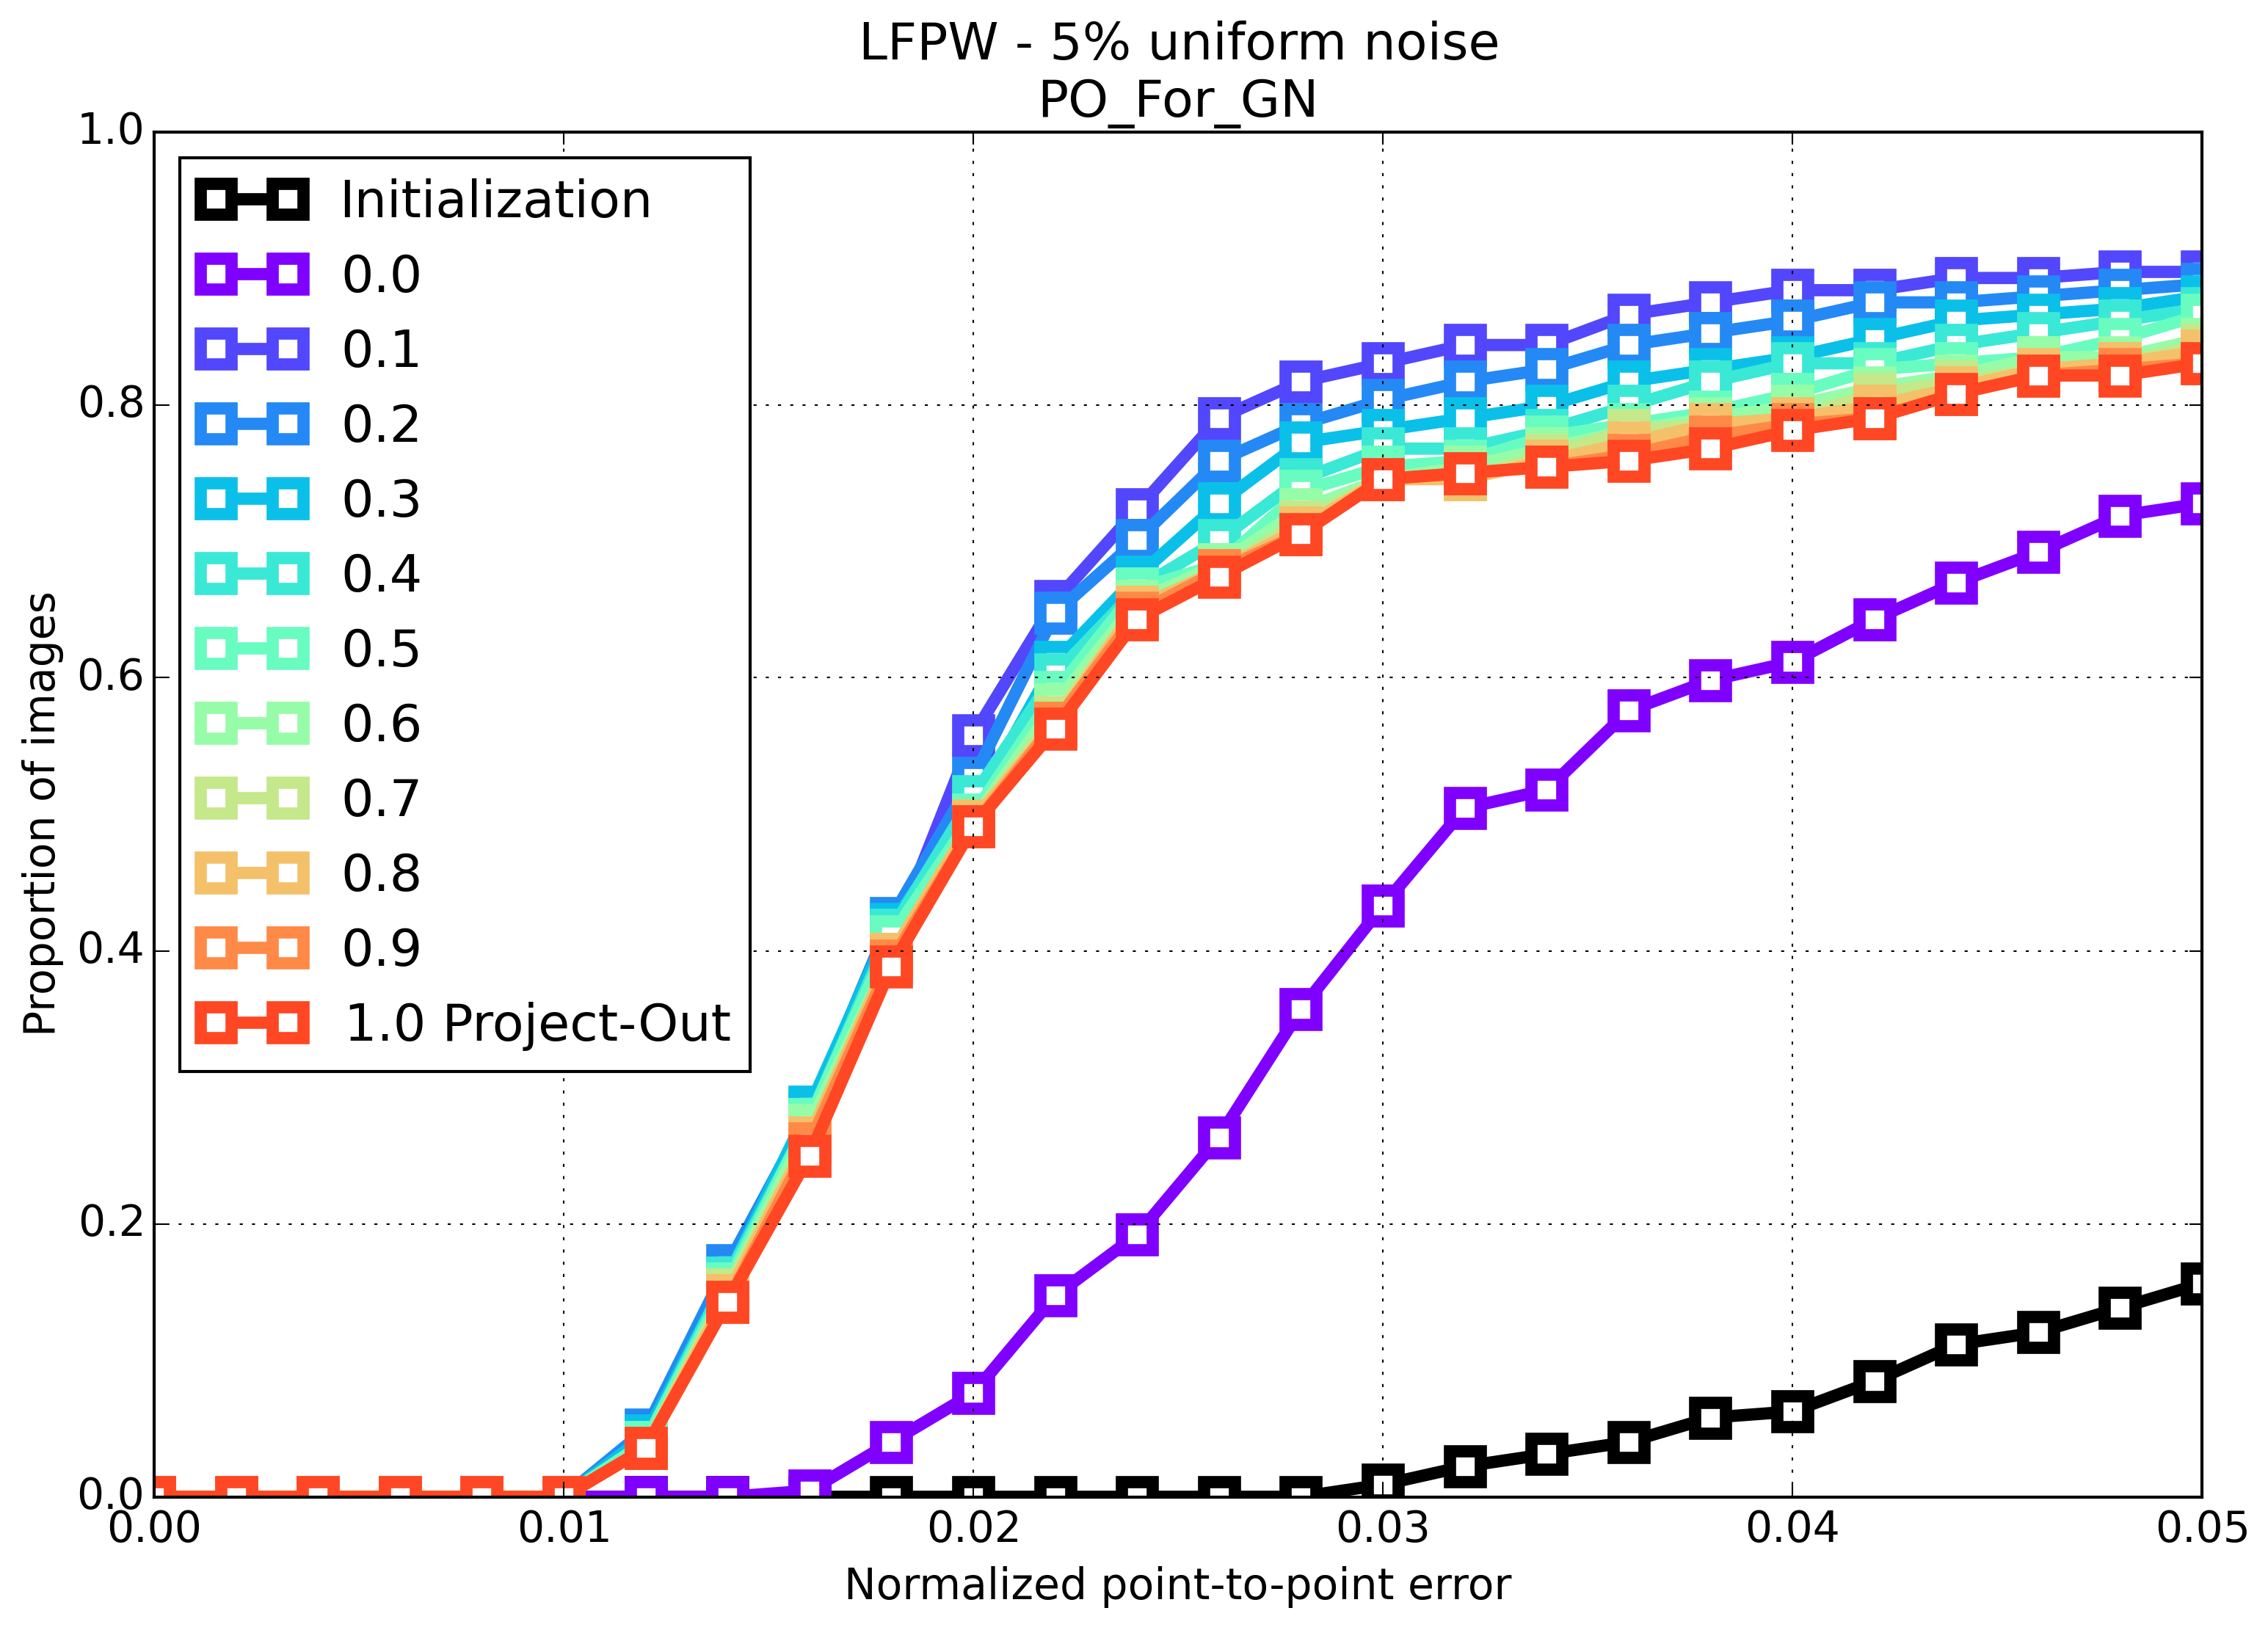
\includegraphics[width=\textwidth]{experiments/rho/ced_po_for_gn_5.png}
	    \caption{CED on the LFPW test dataset for Project-Out Forward Gauss-Newton algorithms for different values of $\rho$ and $\gamma$ and initialized with $5\%$ noise.}
	    \label{fig:ced_po_for_gn}
	\end{subfigure}
	\hfill
	\begin{subfigure}{0.48\textwidth}
	    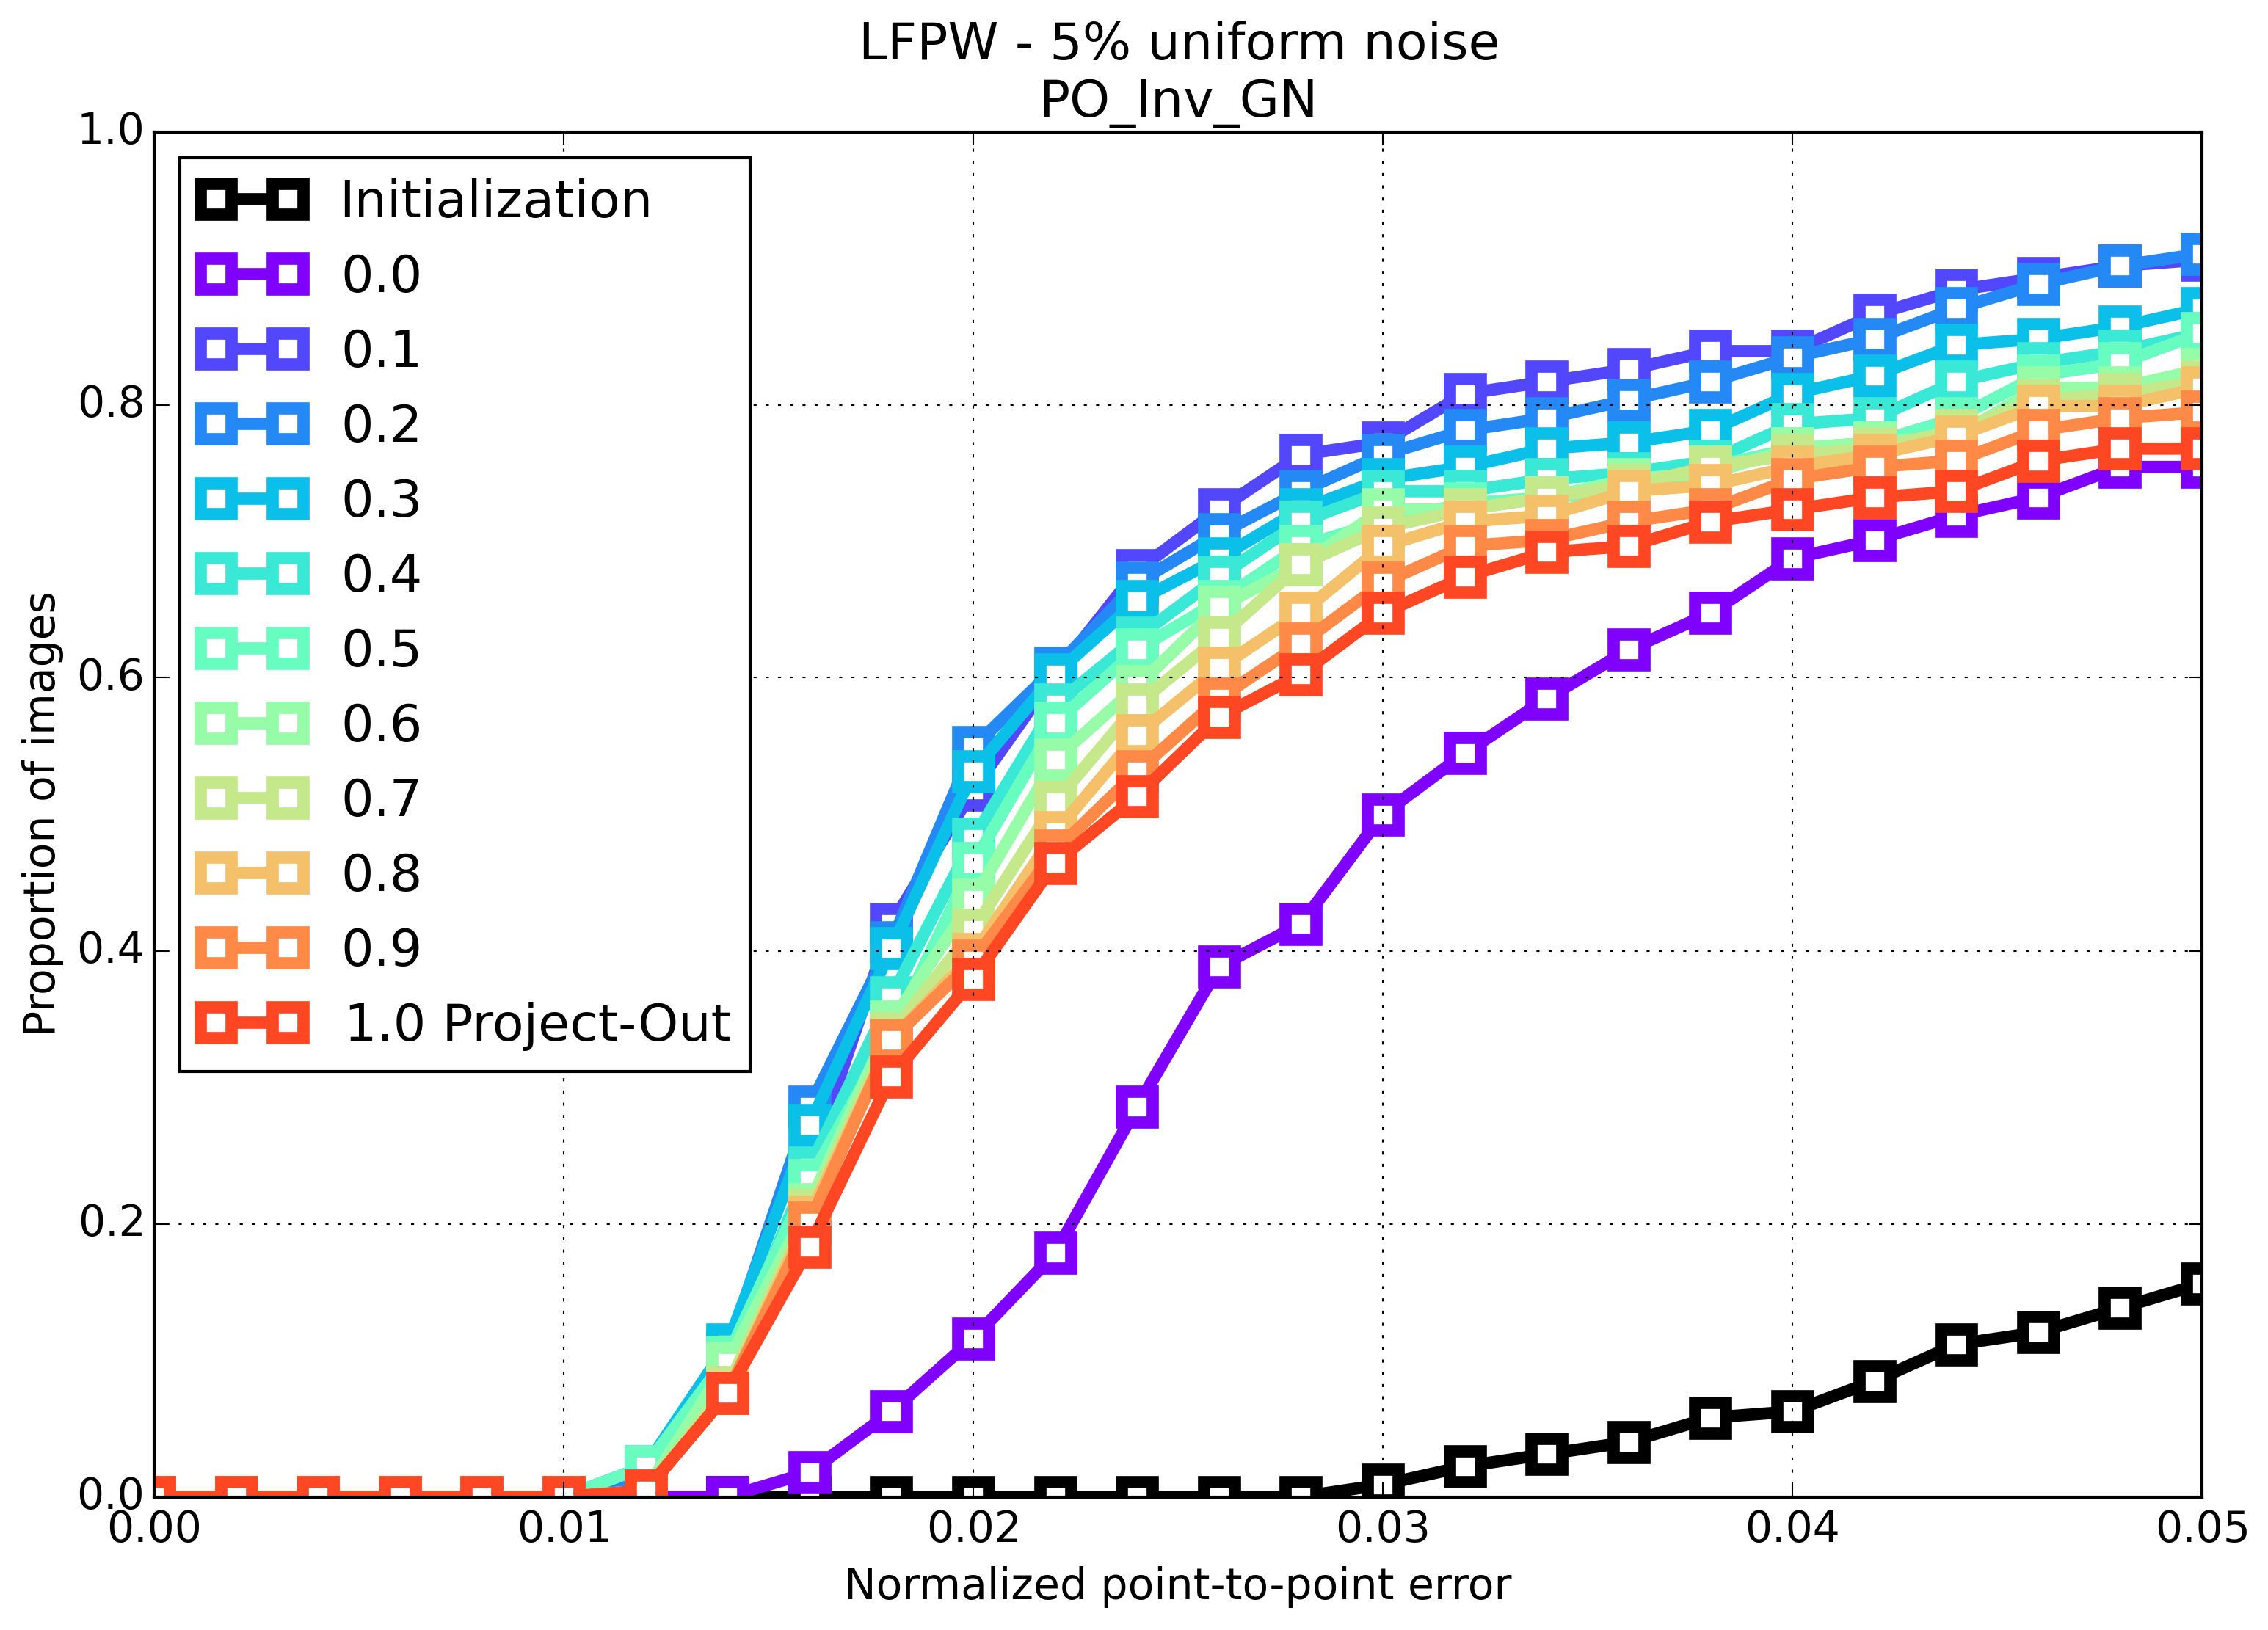
\includegraphics[width=\textwidth]{experiments/rho/ced_po_inv_gn_5.png}
	    \caption{CED on the LFPW test dataset for Project-Out Inverse Gauss-Newton algorithms for different values of $\rho$ and $\gamma$ and initialized with $5\%$ noise.}
	    \label{fig:ced_po_inv_gn}
	\end{subfigure}
	\par\bigskip
	\begin{subfigure}{0.48\textwidth}
	    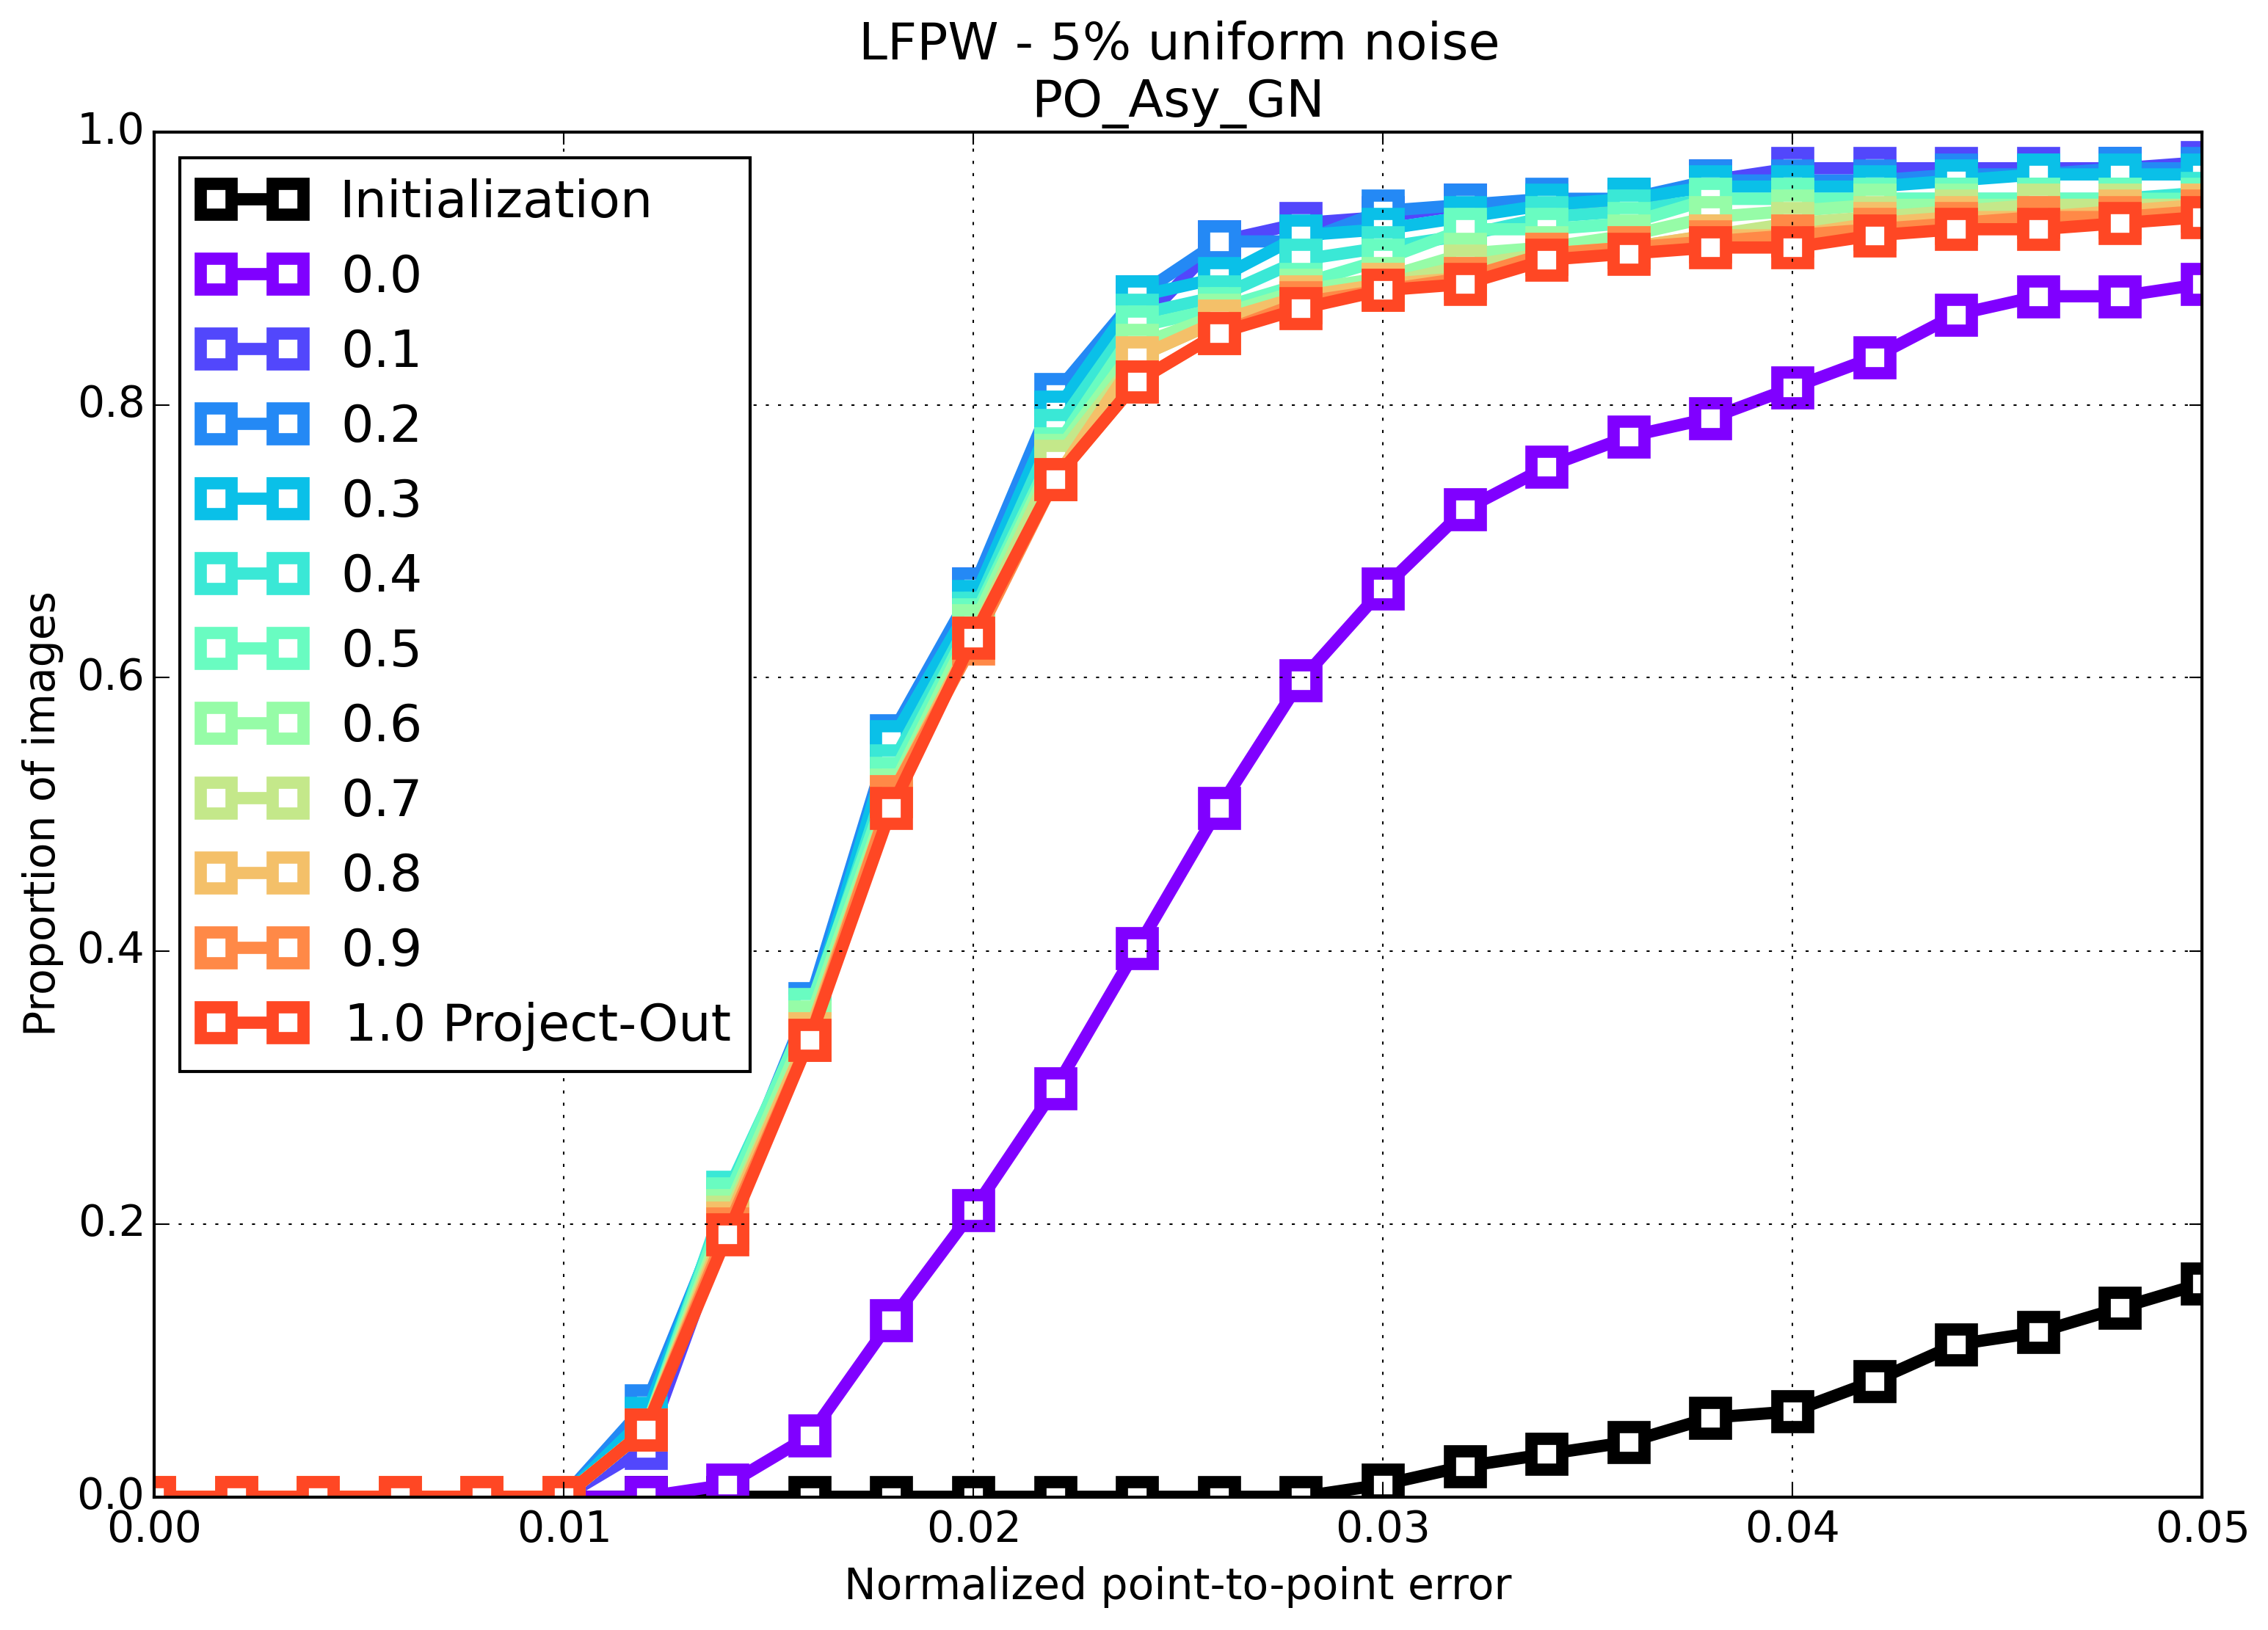
\includegraphics[width=\textwidth]{experiments/rho/ced_po_asy_gn_5.png}
	    \caption{CED on the LFPW test dataset for Project-Out Asymmetric Gauss-Newton algorithms for different values of $\rho$ and $\gamma$ and initialized with $5\%$ noise.}
	    \label{fig:ced_po_asy_gn}
	\end{subfigure}
	\hfill
	\begin{subfigure}{0.48\textwidth}
	    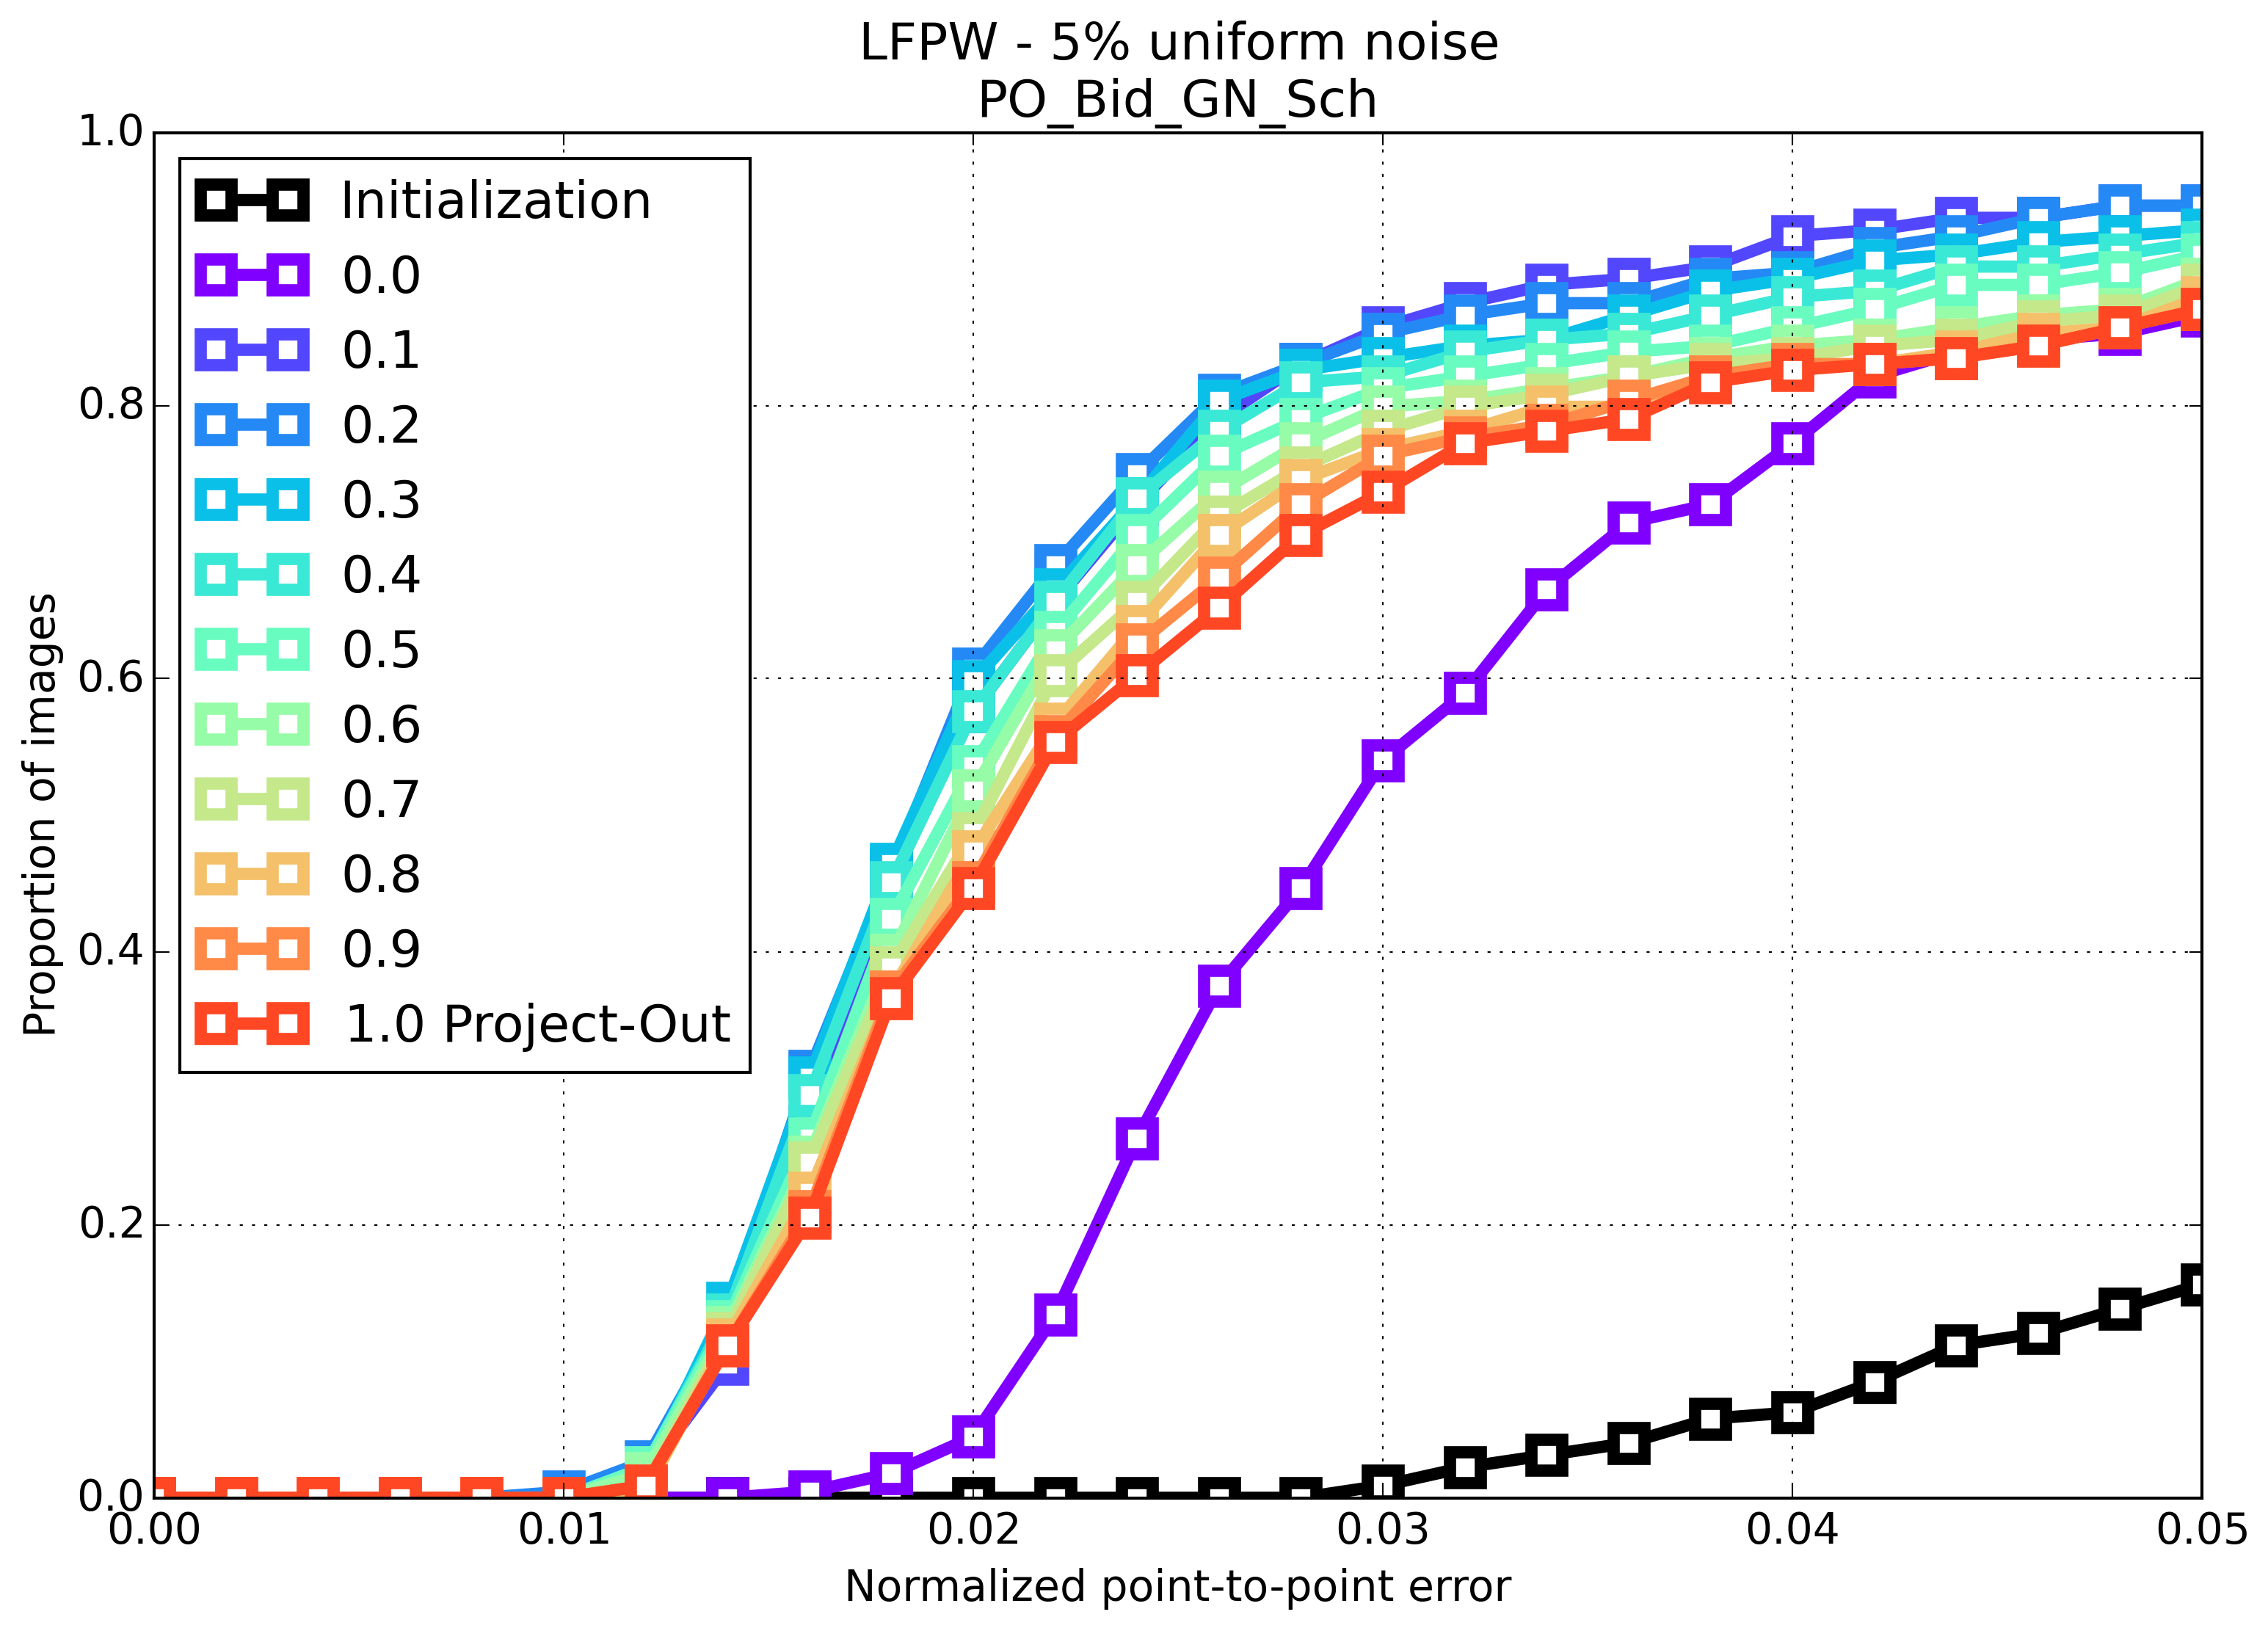
\includegraphics[width=\textwidth]{experiments/rho/ced_po_bid_gn_5.png}
	    \caption{CED on the LFPW test dataset for Project-Out Bidirectional Gauss-Newton algorithms for different values of $\rho$ and $\gamma$ and initialized with $5\%$ noise.}
	    \label{fig:ced_po_bid_gn}
	\end{subfigure}
	\caption{Results quantifying the effect of varying the value of the parameters $\rho$ and $\gamma$ in Project-Out Gauss-Newton algorithms.}
	\label{fig:rho}
\end{figure*}

% \begin{figure}[h!]
% 	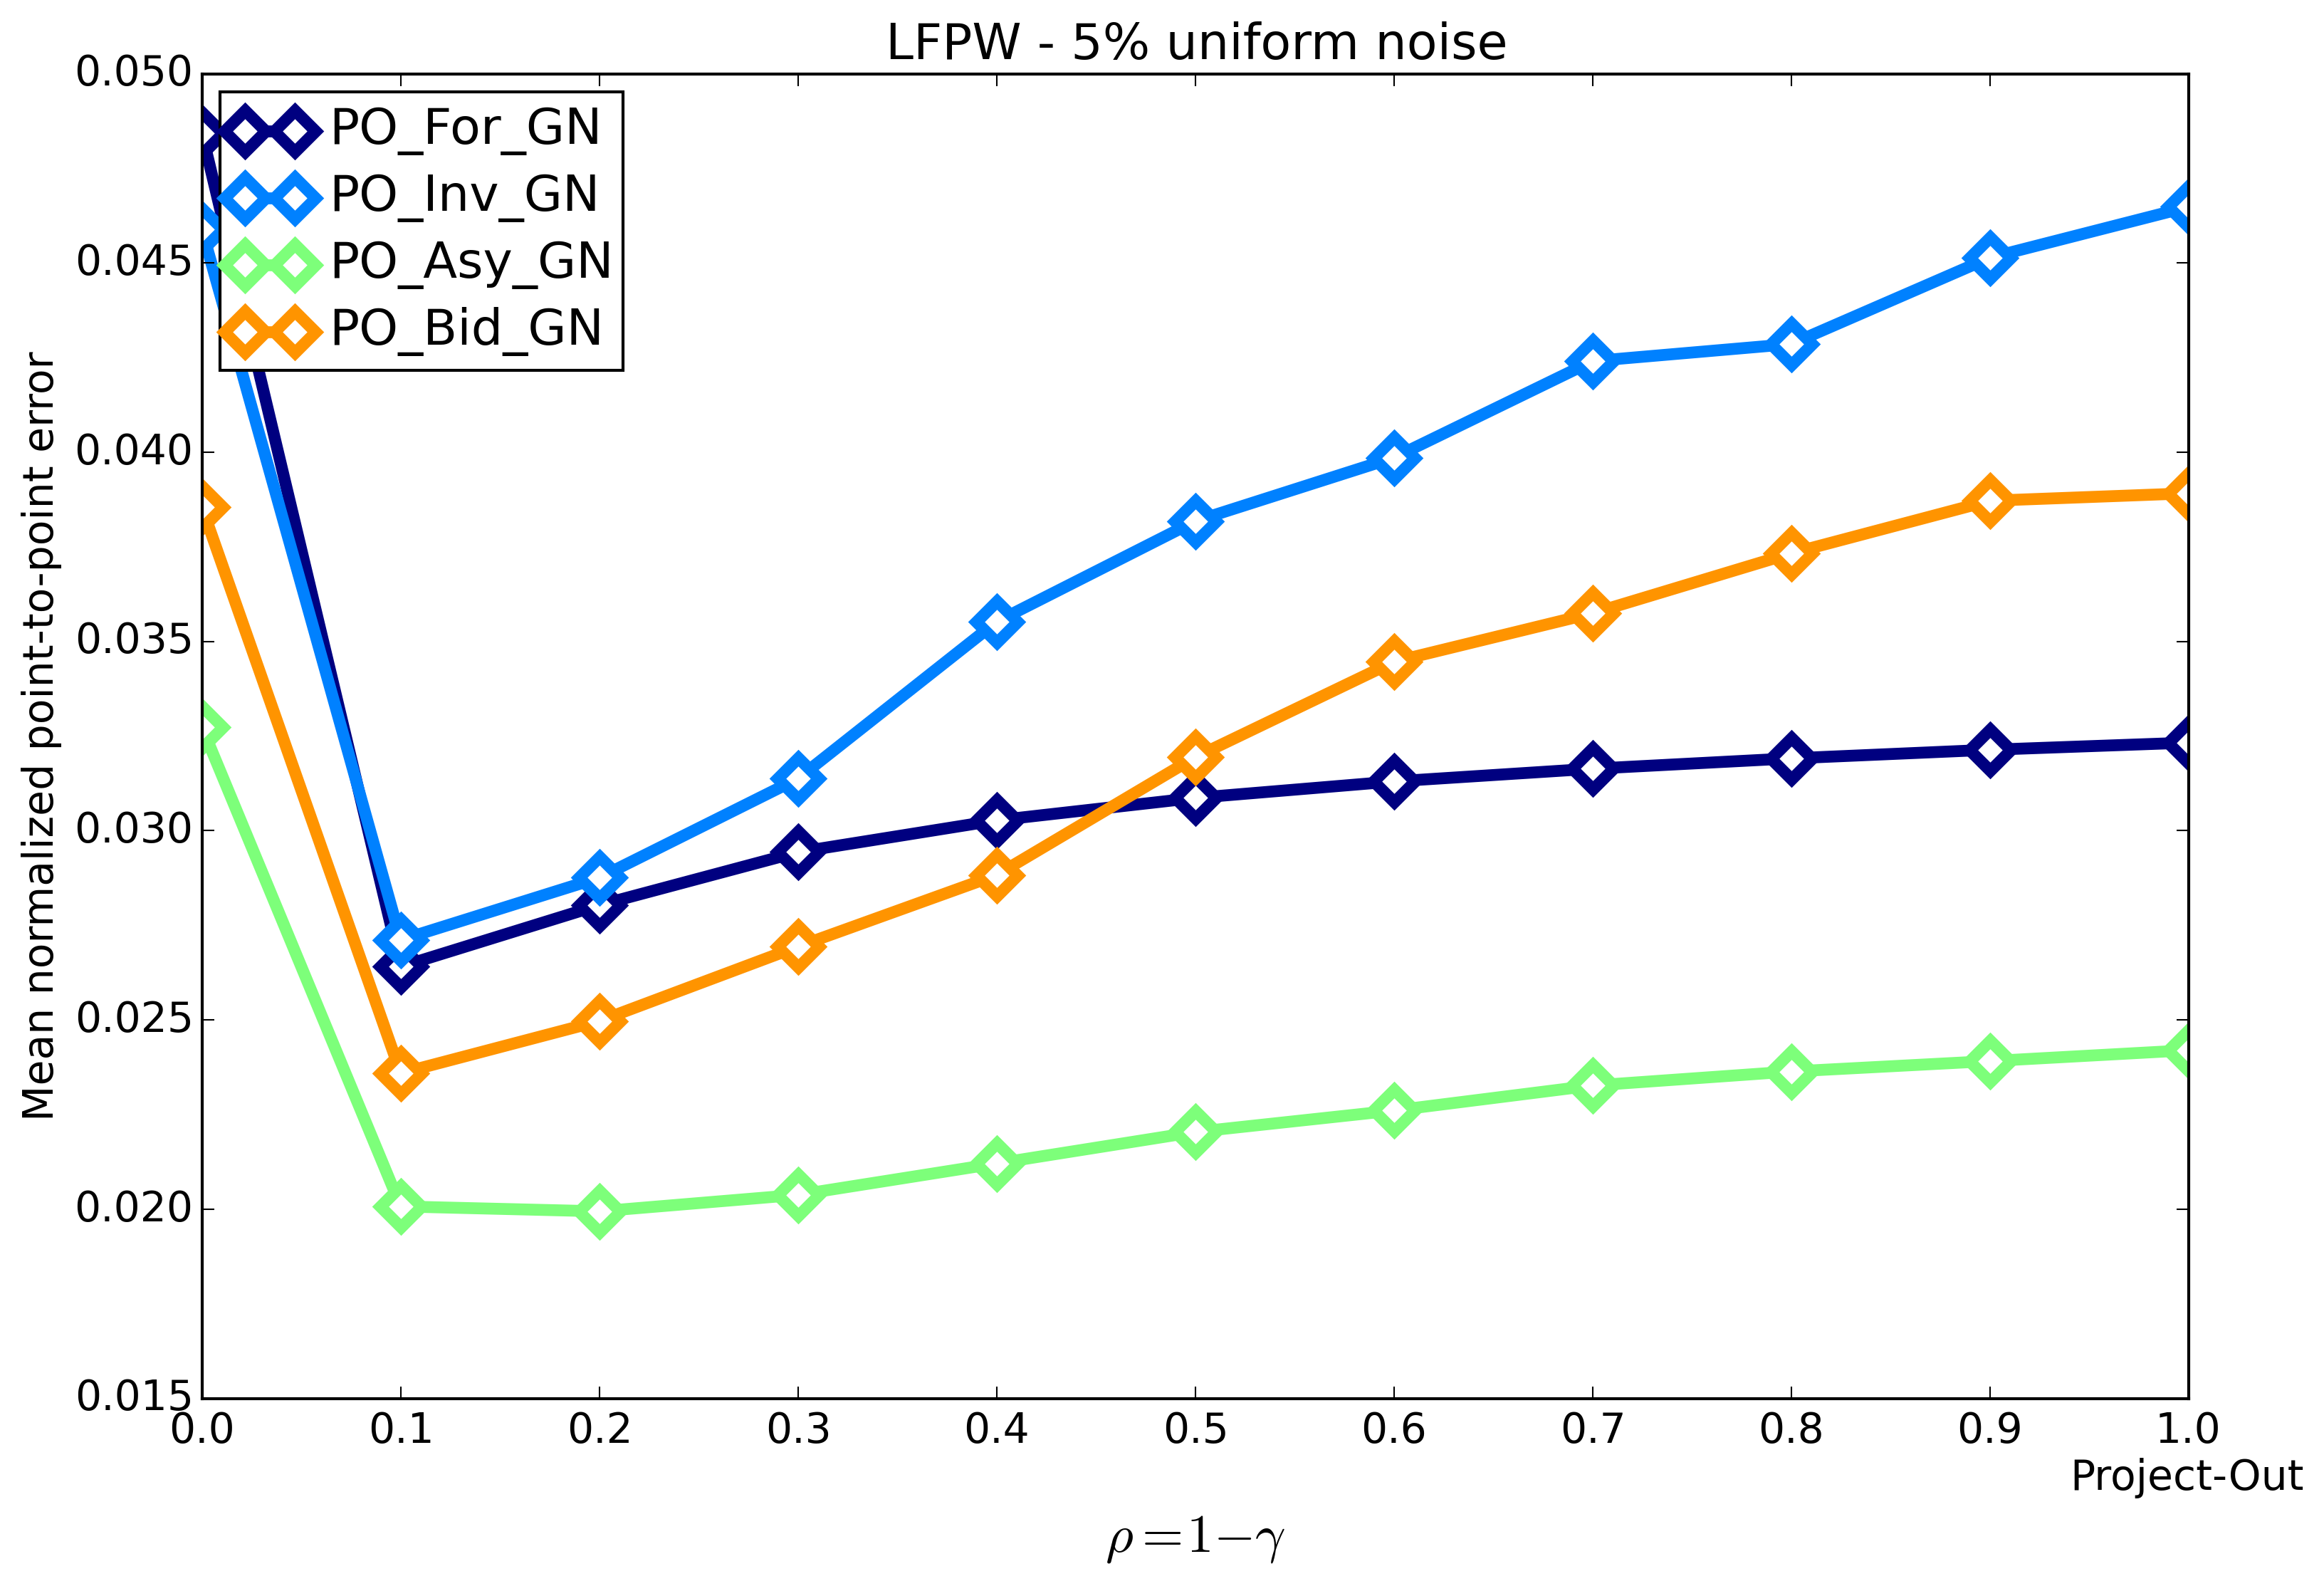
\includegraphics[width=0.48\textwidth]{experiments/rho/mean_error_vs_rho_5.png}
%     \caption{Mean normalized point-to-point error vs rho on the LFPW test dataset for all PO Gauss-Newton algorithms initialized with $5\%$ uniform noise.}
%     \label{fig:rho_5}
% \end{figure}


\subsection{Optimal asymmetric composition}

This experiment quantifies the effect that varying the value of the parameters $\alpha \in [0, 1]$ and $\beta = 1 -\alpha$ in Equation \ref{eq:ssd_ac} has in the fitting accuracy obtained by the asymmetric algorithms. Note that for $\alpha=1$, $\beta=0$ and $\alpha=0$, $\beta=1$ these algorithms reduce to their forward and inverse versions respectively. Remember that, in previous experiments, we used the symmetric case $\alpha=\beta=0.5$ to generate the results reported for \emph{Asymmetric Gauss-Newton} algorithms.

We again repeat the experimental set up described in the first experiments and report the fitting accuracy obtained by the Project Out and SSD Asymmetric Gauss-Newton algorithms for different values of the parameters $\alpha$ and $\beta$. Results are shown in Figure \ref{fig:alpha}. For the \emph{BPO Asymmetric} algorithm, the best results are obtain by setting $\alpha=0.4$, $\beta=0.6$, Figures \ref{fig:asy_gn_vs_alpha_5} (top) and \ref{fig:ced_po_asy_gn_5}. These results slightly outperform those obtain by the default \emph{Symmetric} algorithm and this particular configuration of the \emph{BPO Asymmetric} algorithm is the best performing one on the LFPW test dataset. For the \emph{SSD Asymmetric Gauss-Newton} algorithm the best results are obtained by setting $\alpha=0.2$, $\beta=0.8$, Figures \ref{fig:asy_gn_vs_alpha_5} (bottom) and \ref{fig:ced_ssd_asy_gn_5}. In this case, the boost in performance with respect to the default \emph{Symmetric} algorithm is significant and, with this particular configuration, the \emph{SSD Asymmetric Gauss-Newton} algorithm is the best performing \emph{SSD} algorithm on the LFPW test dataset, outperforming \emph{Inverse} and \emph{Bidirectional} algorithms.

\begin{figure*}[h!]
	\centering
	\begin{subfigure}{\textwidth}
	    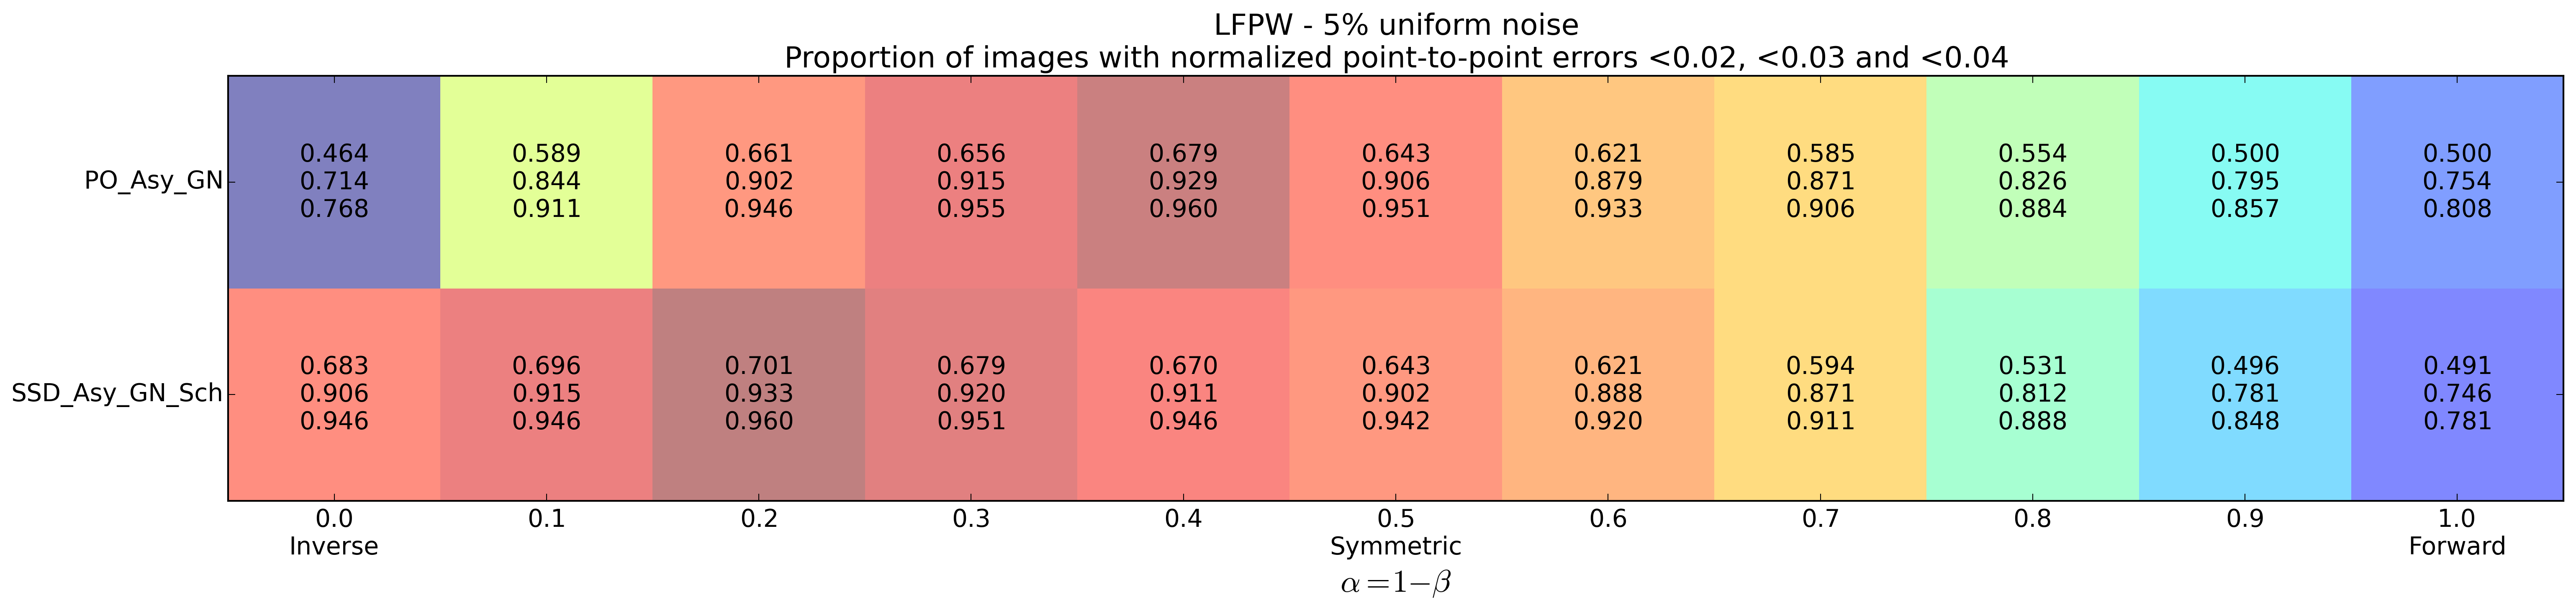
\includegraphics[width=\textwidth]{experiments/alpha/asy_gn_vs_alpha_5.png}
	    \caption{Proportion of images with normalized point-to-point errors smaller than $0.02$, $0.03$ and $0.04$ for the Project-Out and SSD Asymmetric Gauss-Newton algorithms values of $\alpha$ and $\beta$ and initialized with $5\%$ noise.}
	    \label{fig:asy_gn_vs_alpha_5}
	\end{subfigure}
	\par\bigskip\bigskip
	\begin{subfigure}{0.48\textwidth}
	    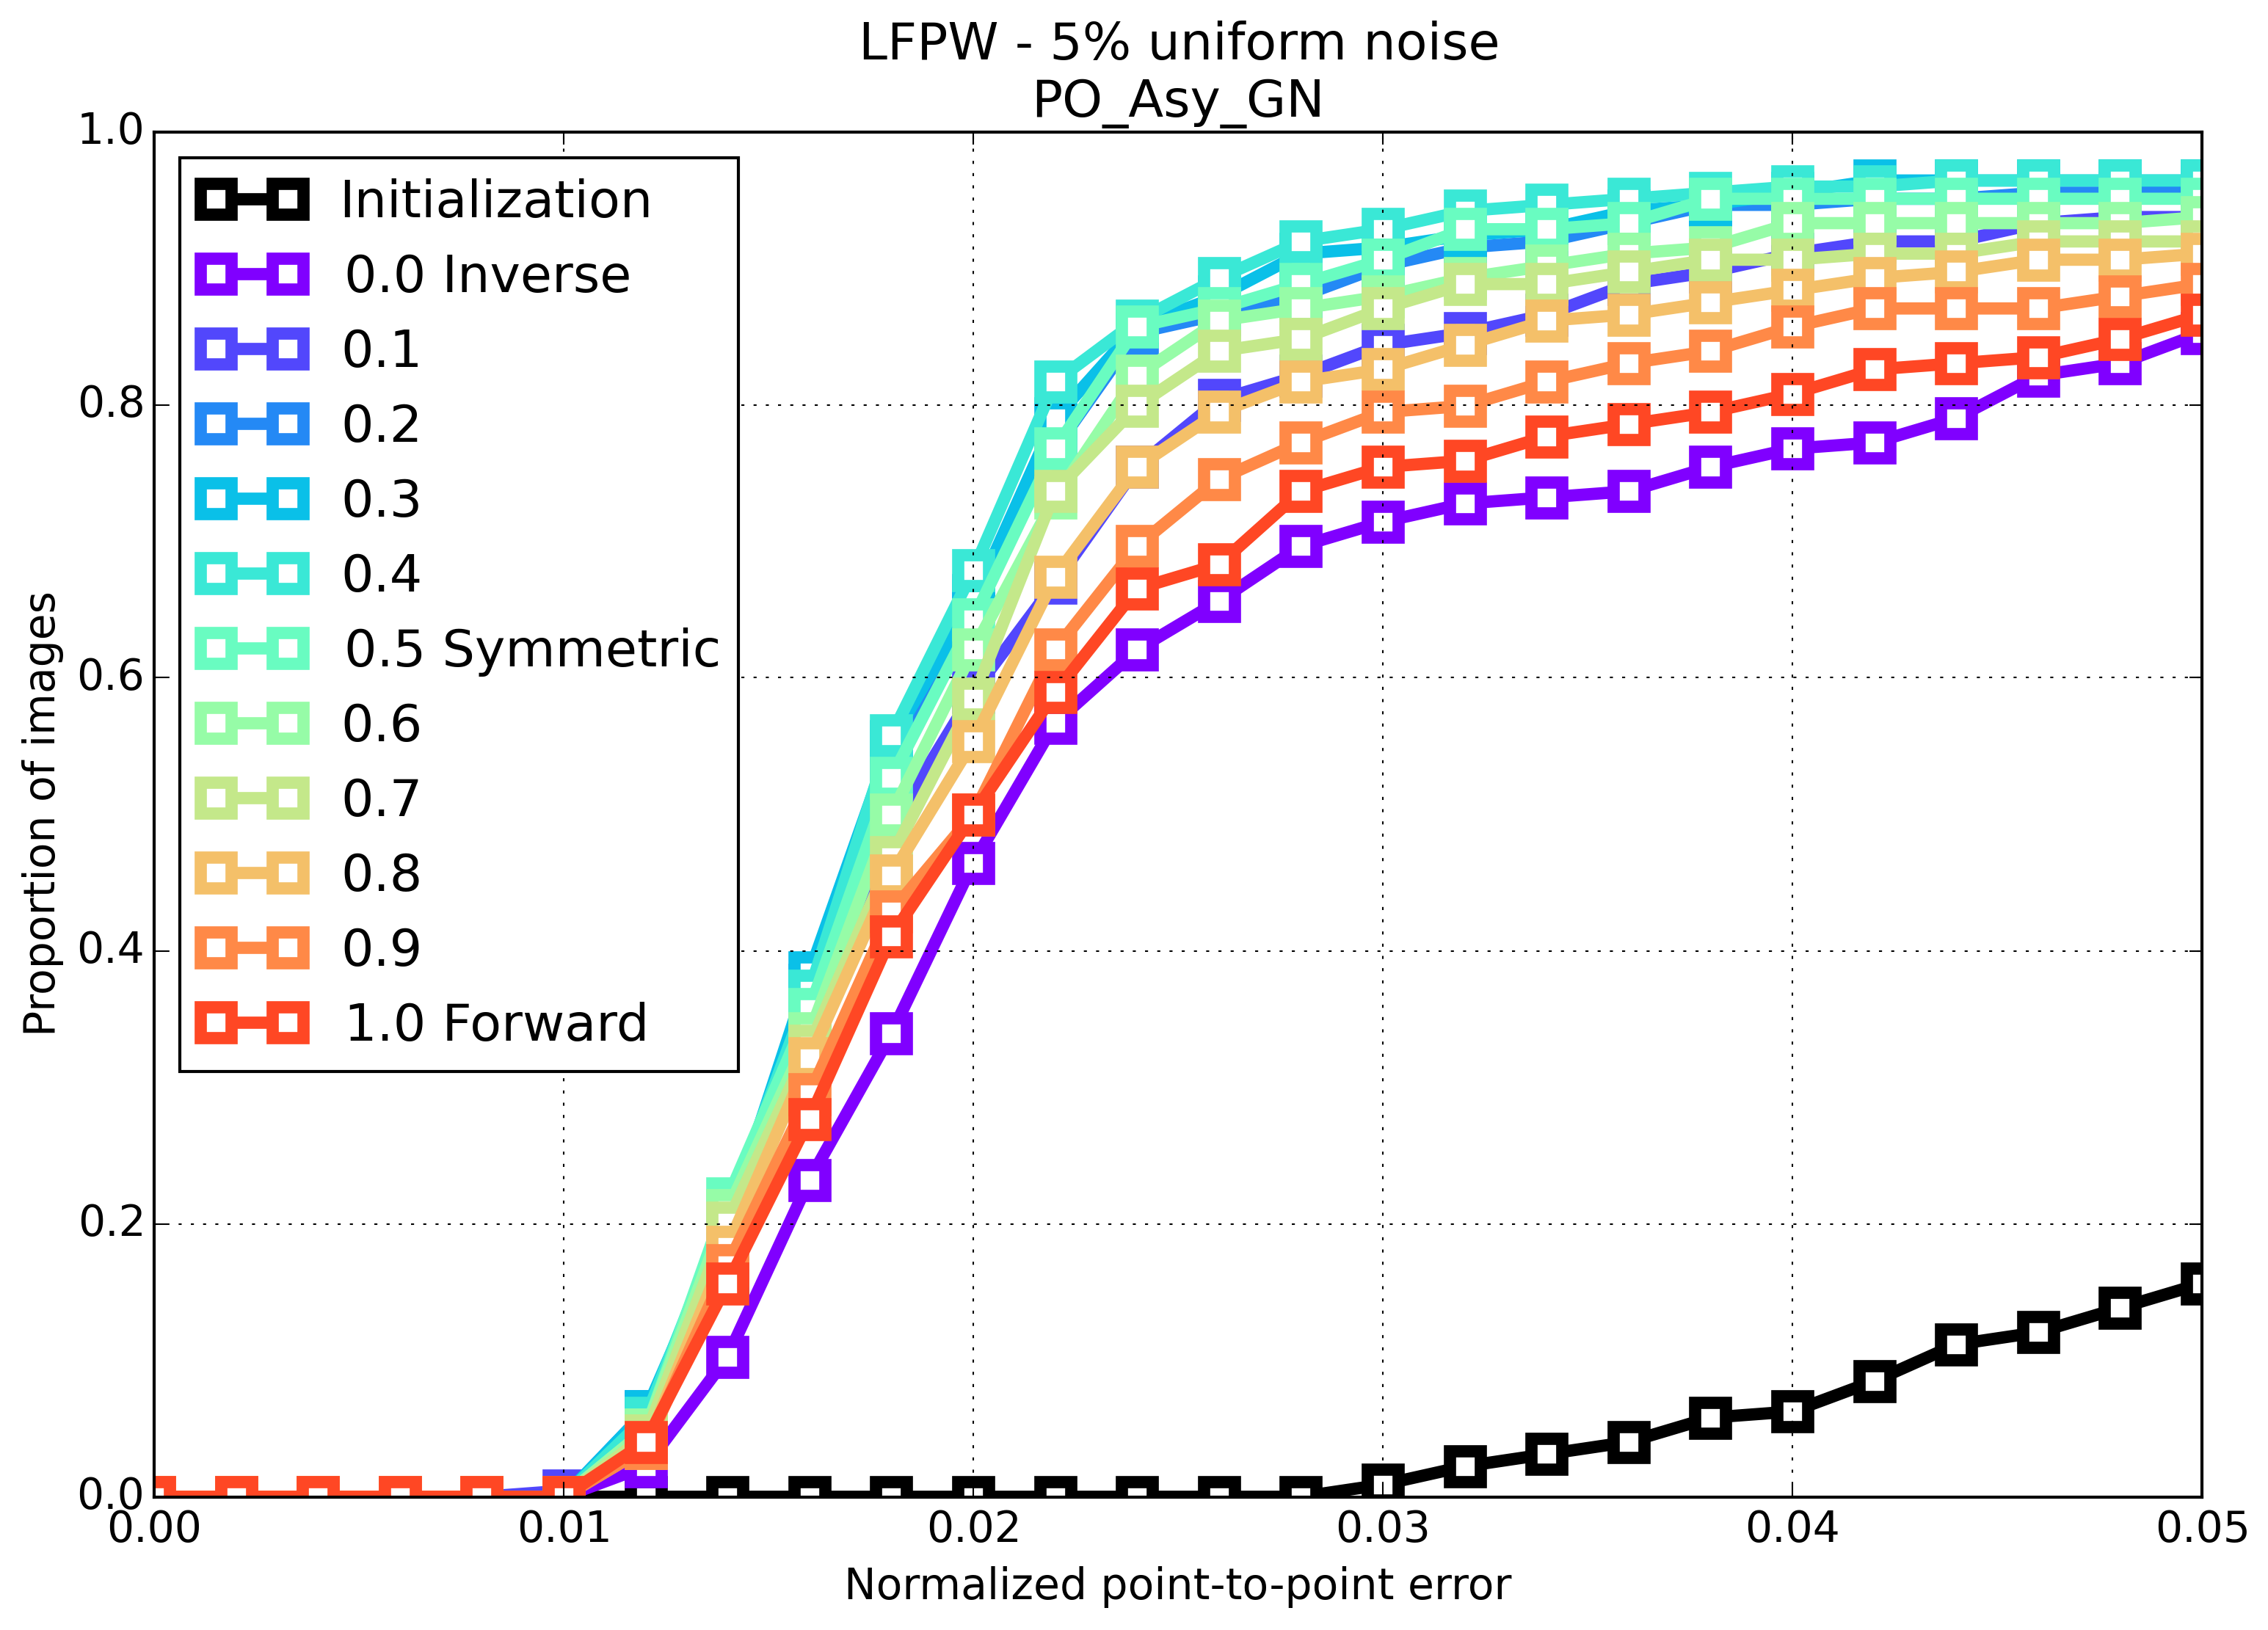
\includegraphics[width=\textwidth]{experiments/alpha/ced_po_asy_gn_5.png}
	    \caption{CED on the LFPW test dataset for Project-Out Asymmetric Gauss-Newton algorithm for different values of $\alpha$ and $\beta$ and initialized with $5\%$ noise.}
	    \label{fig:ced_po_asy_gn_5}
	\end{subfigure}
	\hfill
	\begin{subfigure}{0.48\textwidth}
	    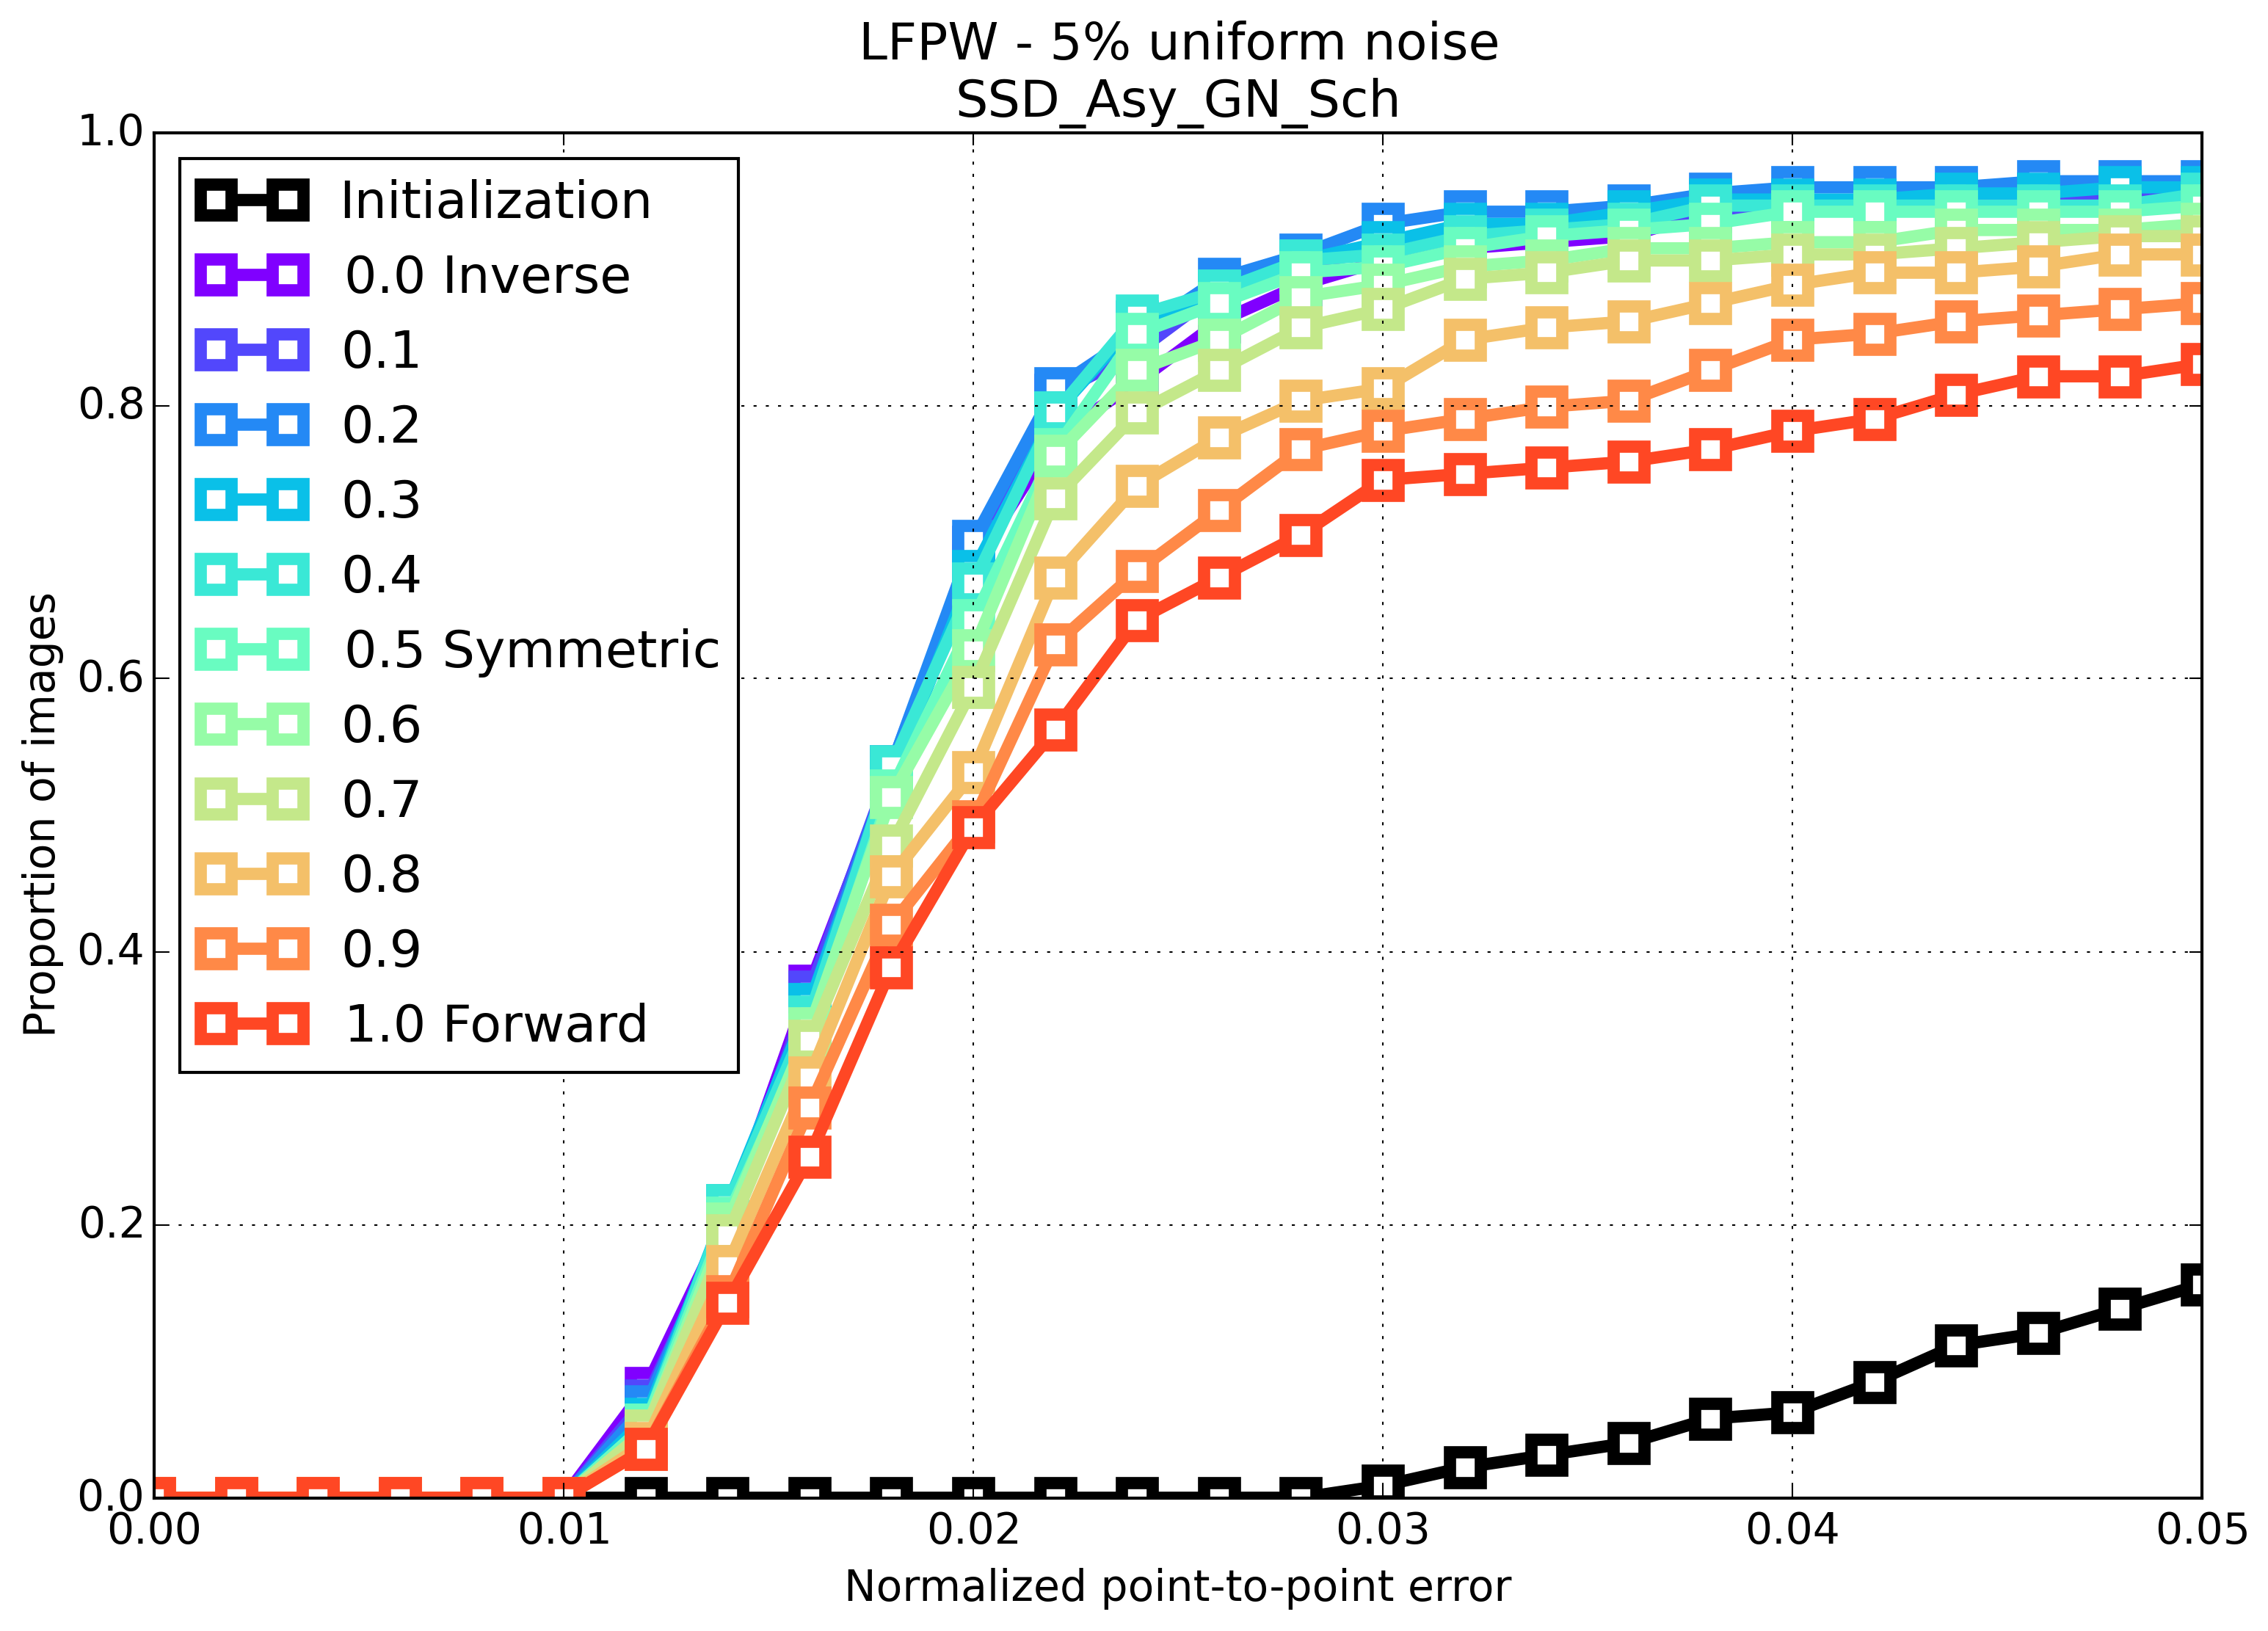
\includegraphics[width=\textwidth]{experiments/alpha/ced_ssd_asy_gn_5.png}
	    \caption{CED on the LFPW test dataset for the the SSD Asymmetric Gauss-Newton algorithm for different values of $\alpha$ and $\beta$ and initialized with $5\%$ noise.}
	    \label{fig:ced_ssd_asy_gn_5}
	\end{subfigure}
	\caption{Results quantifying the effect of varying the value of the parameters $\alpha$ and $\beta$ in Asymmetric algorithms.}
	\label{fig:alpha}
\end{figure*}

% \begin{figure}[h!]
%     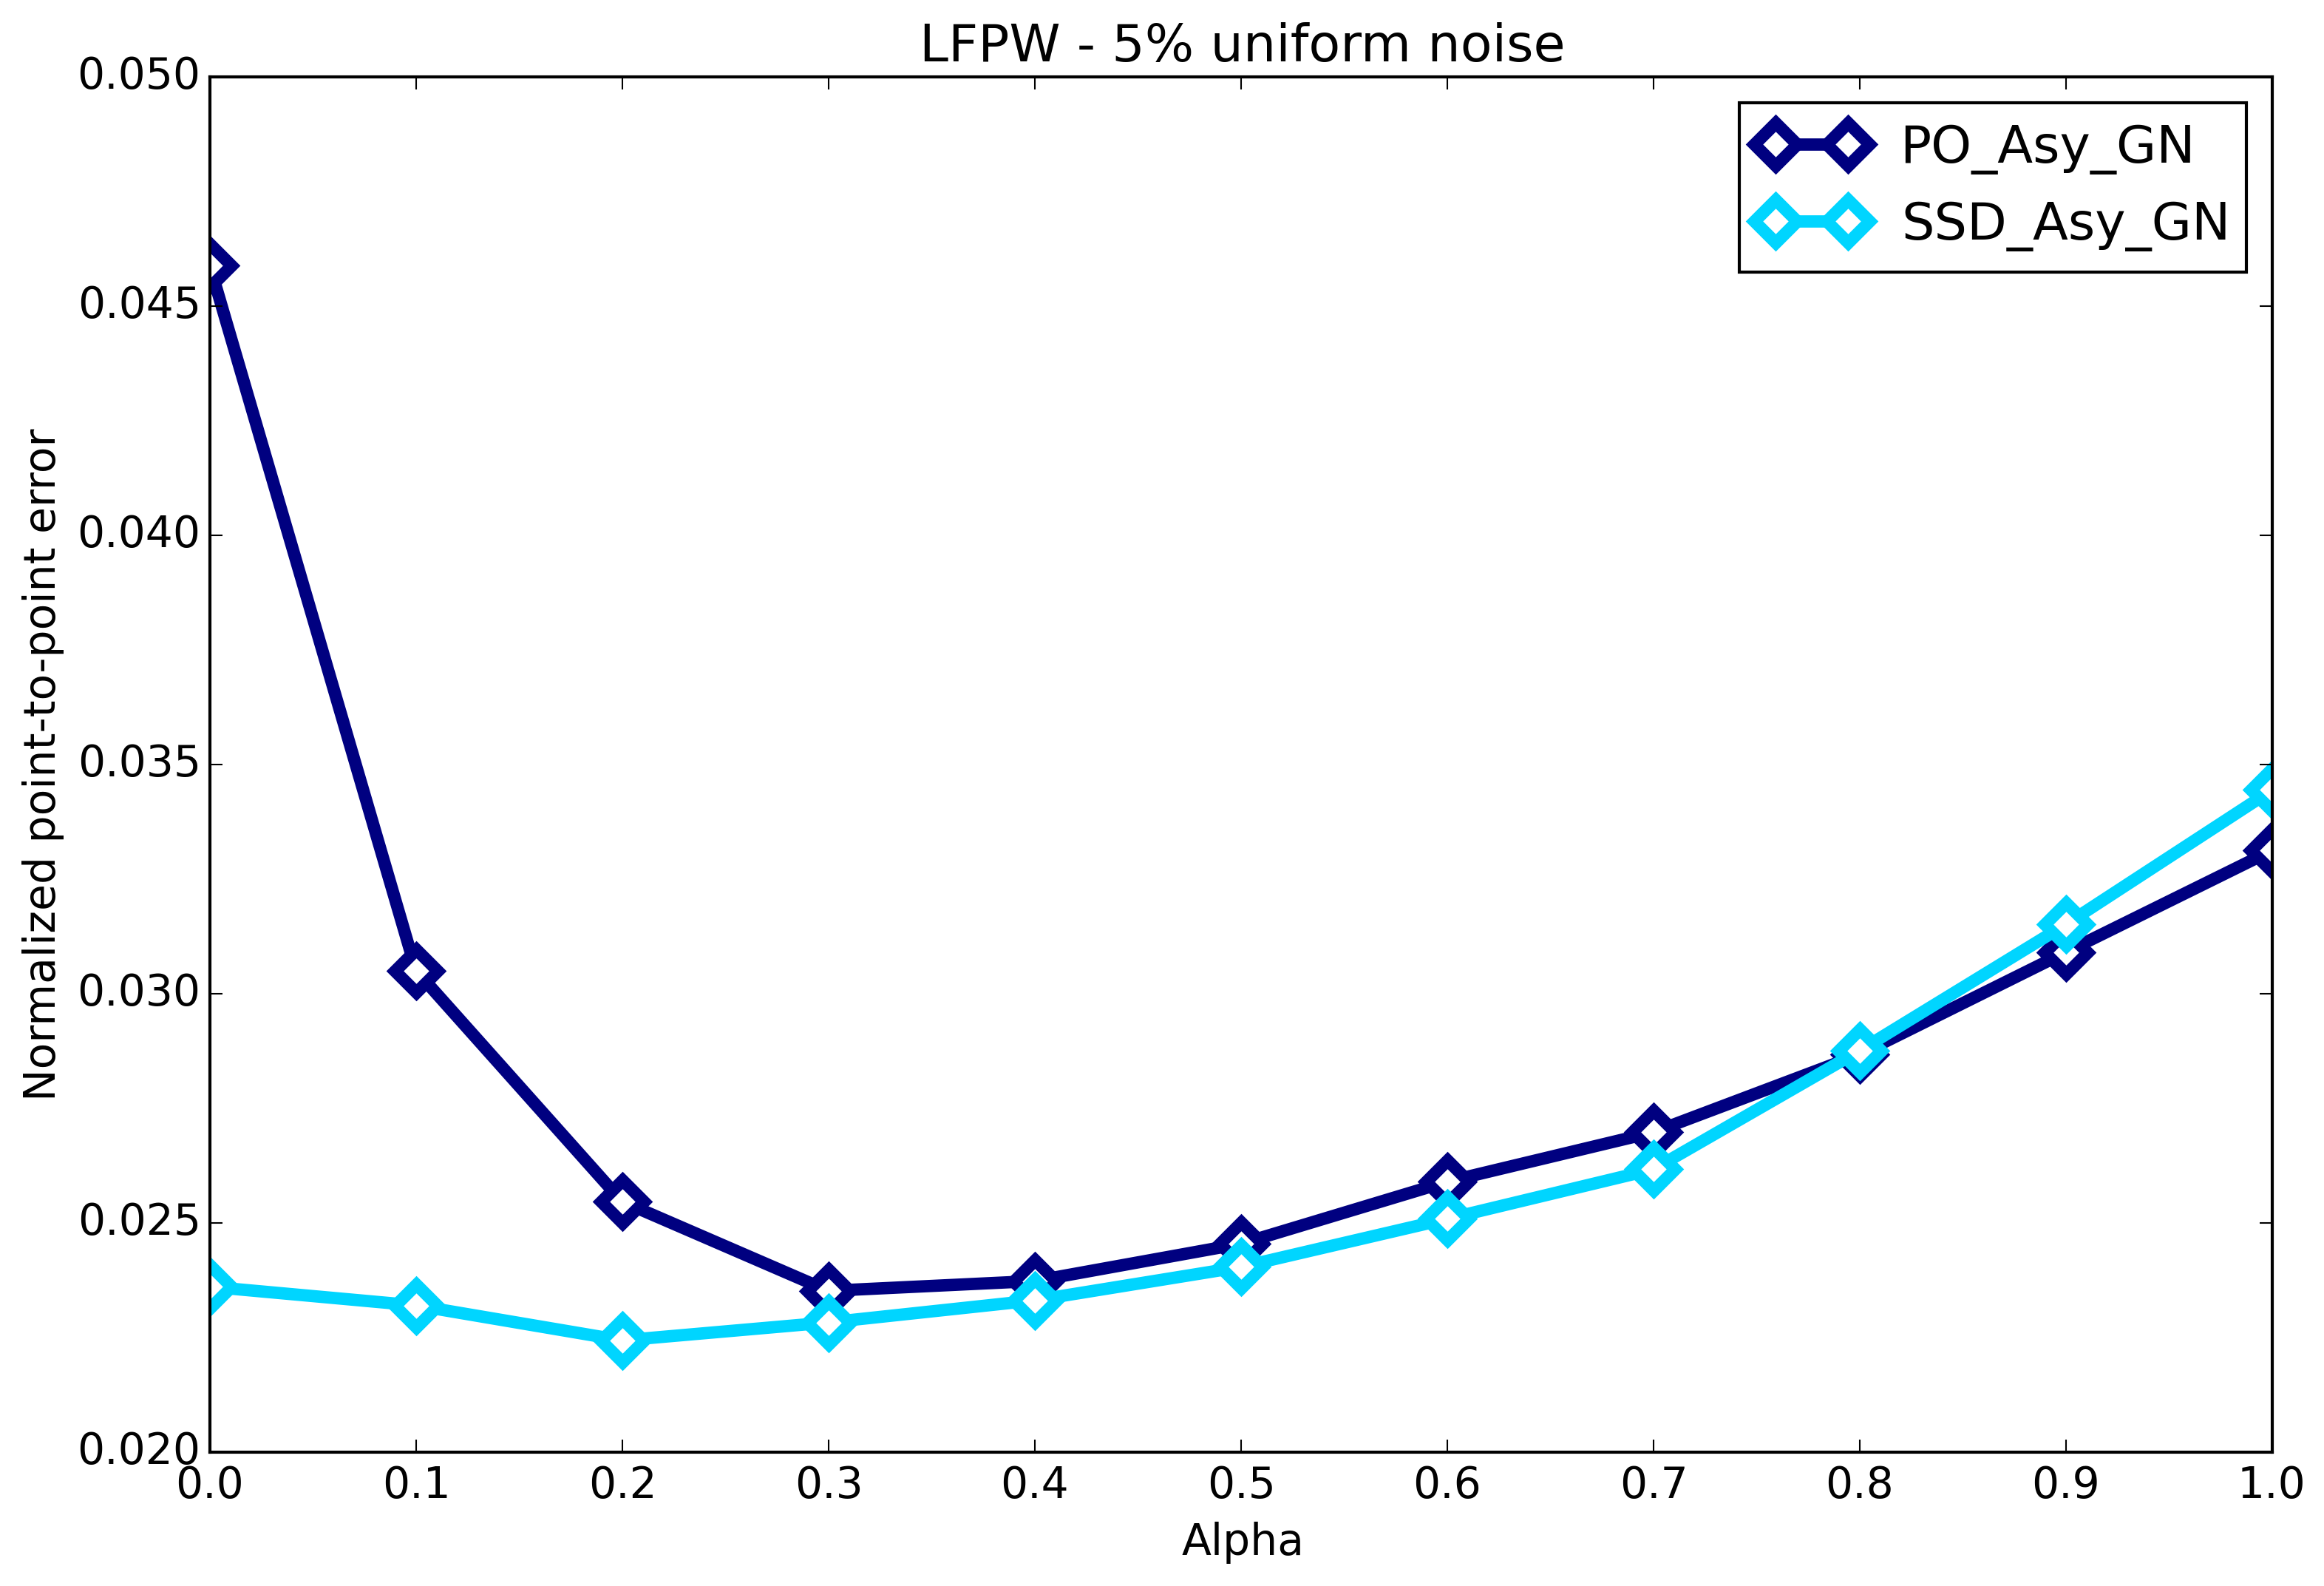
\includegraphics[width=0.48\textwidth]{experiments/alpha/mean_error_vs_alpha_asy_gn_5.png}
%     \caption{Mean normalized point-to-point error vs alpha on the LFPW test dataset for all Asymmetric Gauss-Newton algorithms initialized with $5\%$ uniform noise.}
%     \label{fig:alpha_5}
% \end{figure}


\subsection{Sampling and Number of Iterations}

In this experiment, we explore two different strategies to reduce the running time of the previous CGD algorithms. 

The first one consists of optimizing the SSD and Project-Out cost functions using only a subset of all pixels in the reference frame.In AAMs the total number of pixels on the reference frame, $F$, is typically several orders of magnitude bigger than the number of shape, $n$, and appearance, $m$, components i.e. $F>>m>>n$. Therefore, a significant reduction in the complexity (and running time) of CGD algorithms can be obtained by decreasing the number of pixels that are used to optimize the previous cost functions. To this end, we compare the accuracy obtained by using $100\%$, $50\%$, $25\%$ and $12\%$ of the total number of pixels on the reference frame. Note that, pixels are (approximately) evenly sampled across the reference frame in all cases, Figure \ref{fig:sampling_masks}.

The second strategy consist of simply reducing the number of iterations that each algorithm is run. Based on the figures used to asses the convergence properties of CGD algorithms in previous experiments, we compare the accuracy obtained by running the algorithms for $40 (24 + 16)$ and $20 (12 + 8)$ iterations.

Once more we repeat the experimental set up of the first experiment and report the fitting accuracy obtained by the Project Out and SSD Asymmetric Gauss-Newton algorithms. Result for this experiment are shown in Figure \ref{fig:sampling}. It can be seen that reducing the number of pixels up to $25\%$ while maintaining the original number of iterations to $40$ has little impact on the fitting accuracy achieved by both algorithms while reducing them to $12\%$ has a clear negative impact. In terms of run time, reducing the number of pixels to $50\%$, $25\%$ and $12\%$ offers speed ups of $\sim2.0$x, $\sim2.9$x and $\sim3.7$x for the \emph{BPO} algorithm and of $\sim1.8$x, $\sim2.6$x and $\sim2.8$x for the \emph{SSD} algorithm respectively. 

\begin{figure*}[h!]
	\centering
	\begin{subfigure}{0.48\textwidth}
	    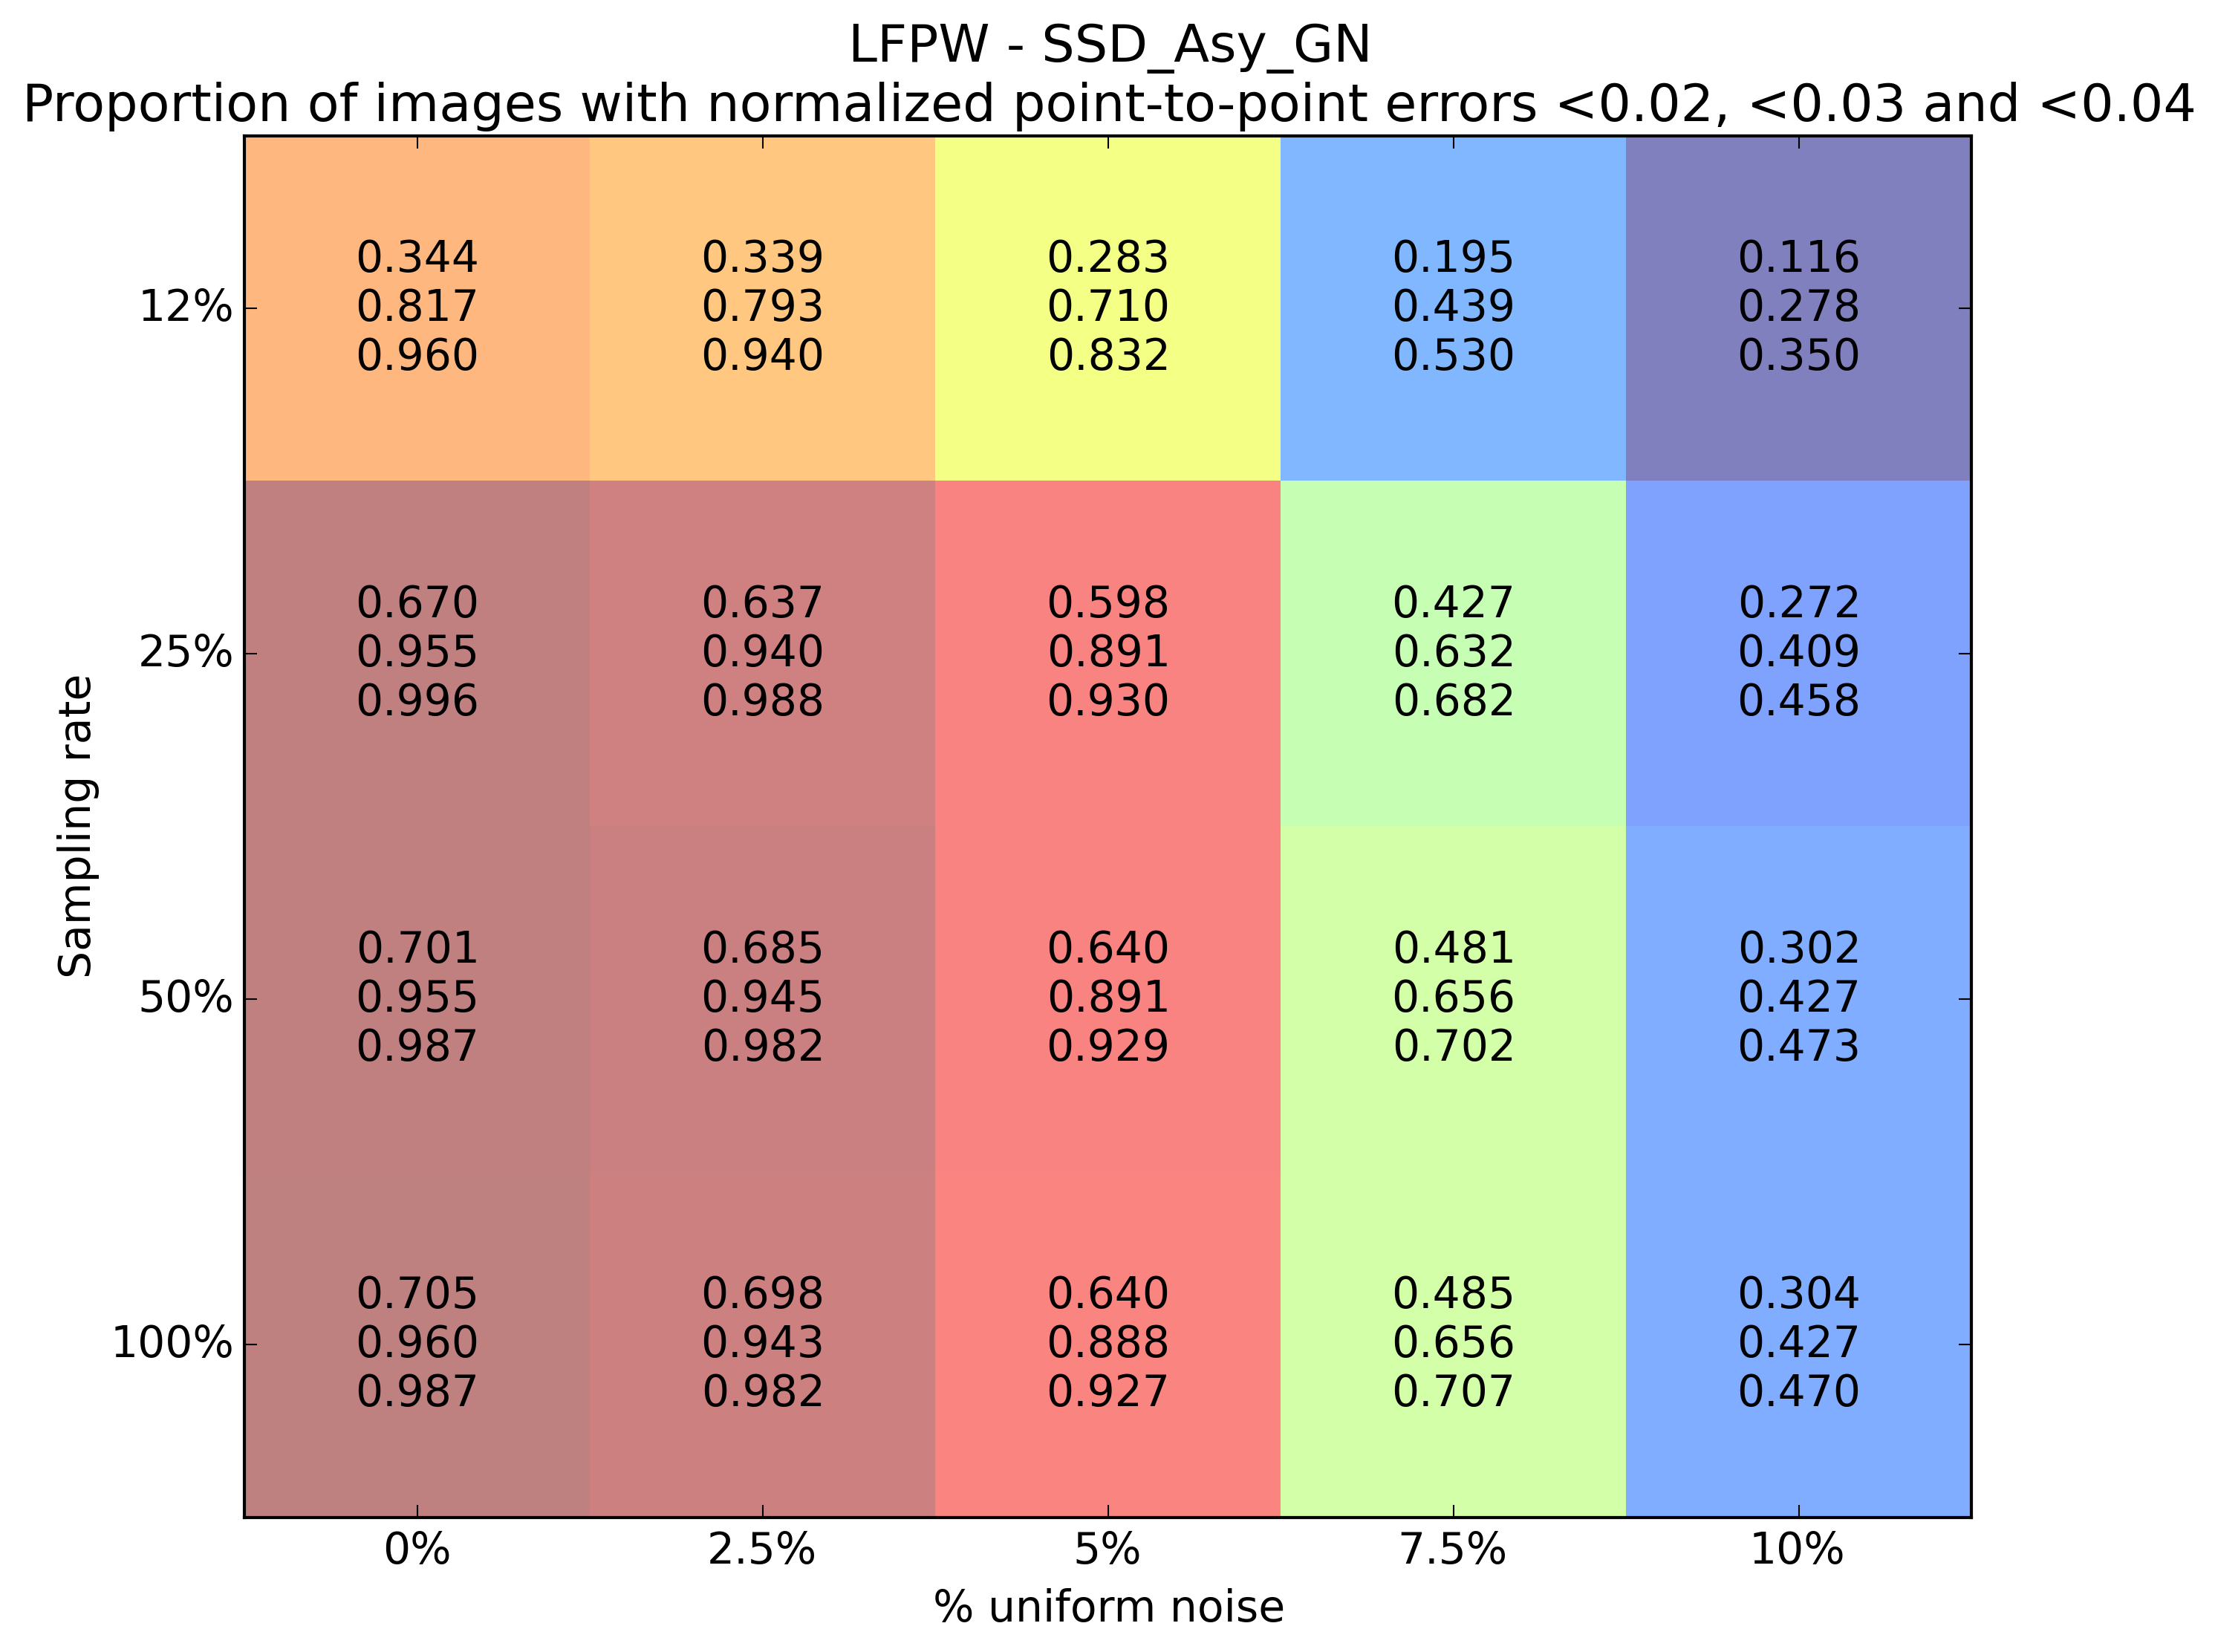
\includegraphics[width=\textwidth]{experiments/sampling/sampling_vs_noise_ssd_asy_gn.png}
	    \caption{Proportion of images with normalized point-to-point errors smaller than $0.02$, $0.03$ and $0.04$ for the SSD Asymmetric Gauss-Newton algorithm using different sampling rates, $40 (24 + 16)$ iterations, and initialized with different amounts of noise.}
	    \label{fig:sampling_vs_noise_ssd_asy_gn}
	\end{subfigure}
	\hfill
	\begin{subfigure}{0.48\textwidth}
	    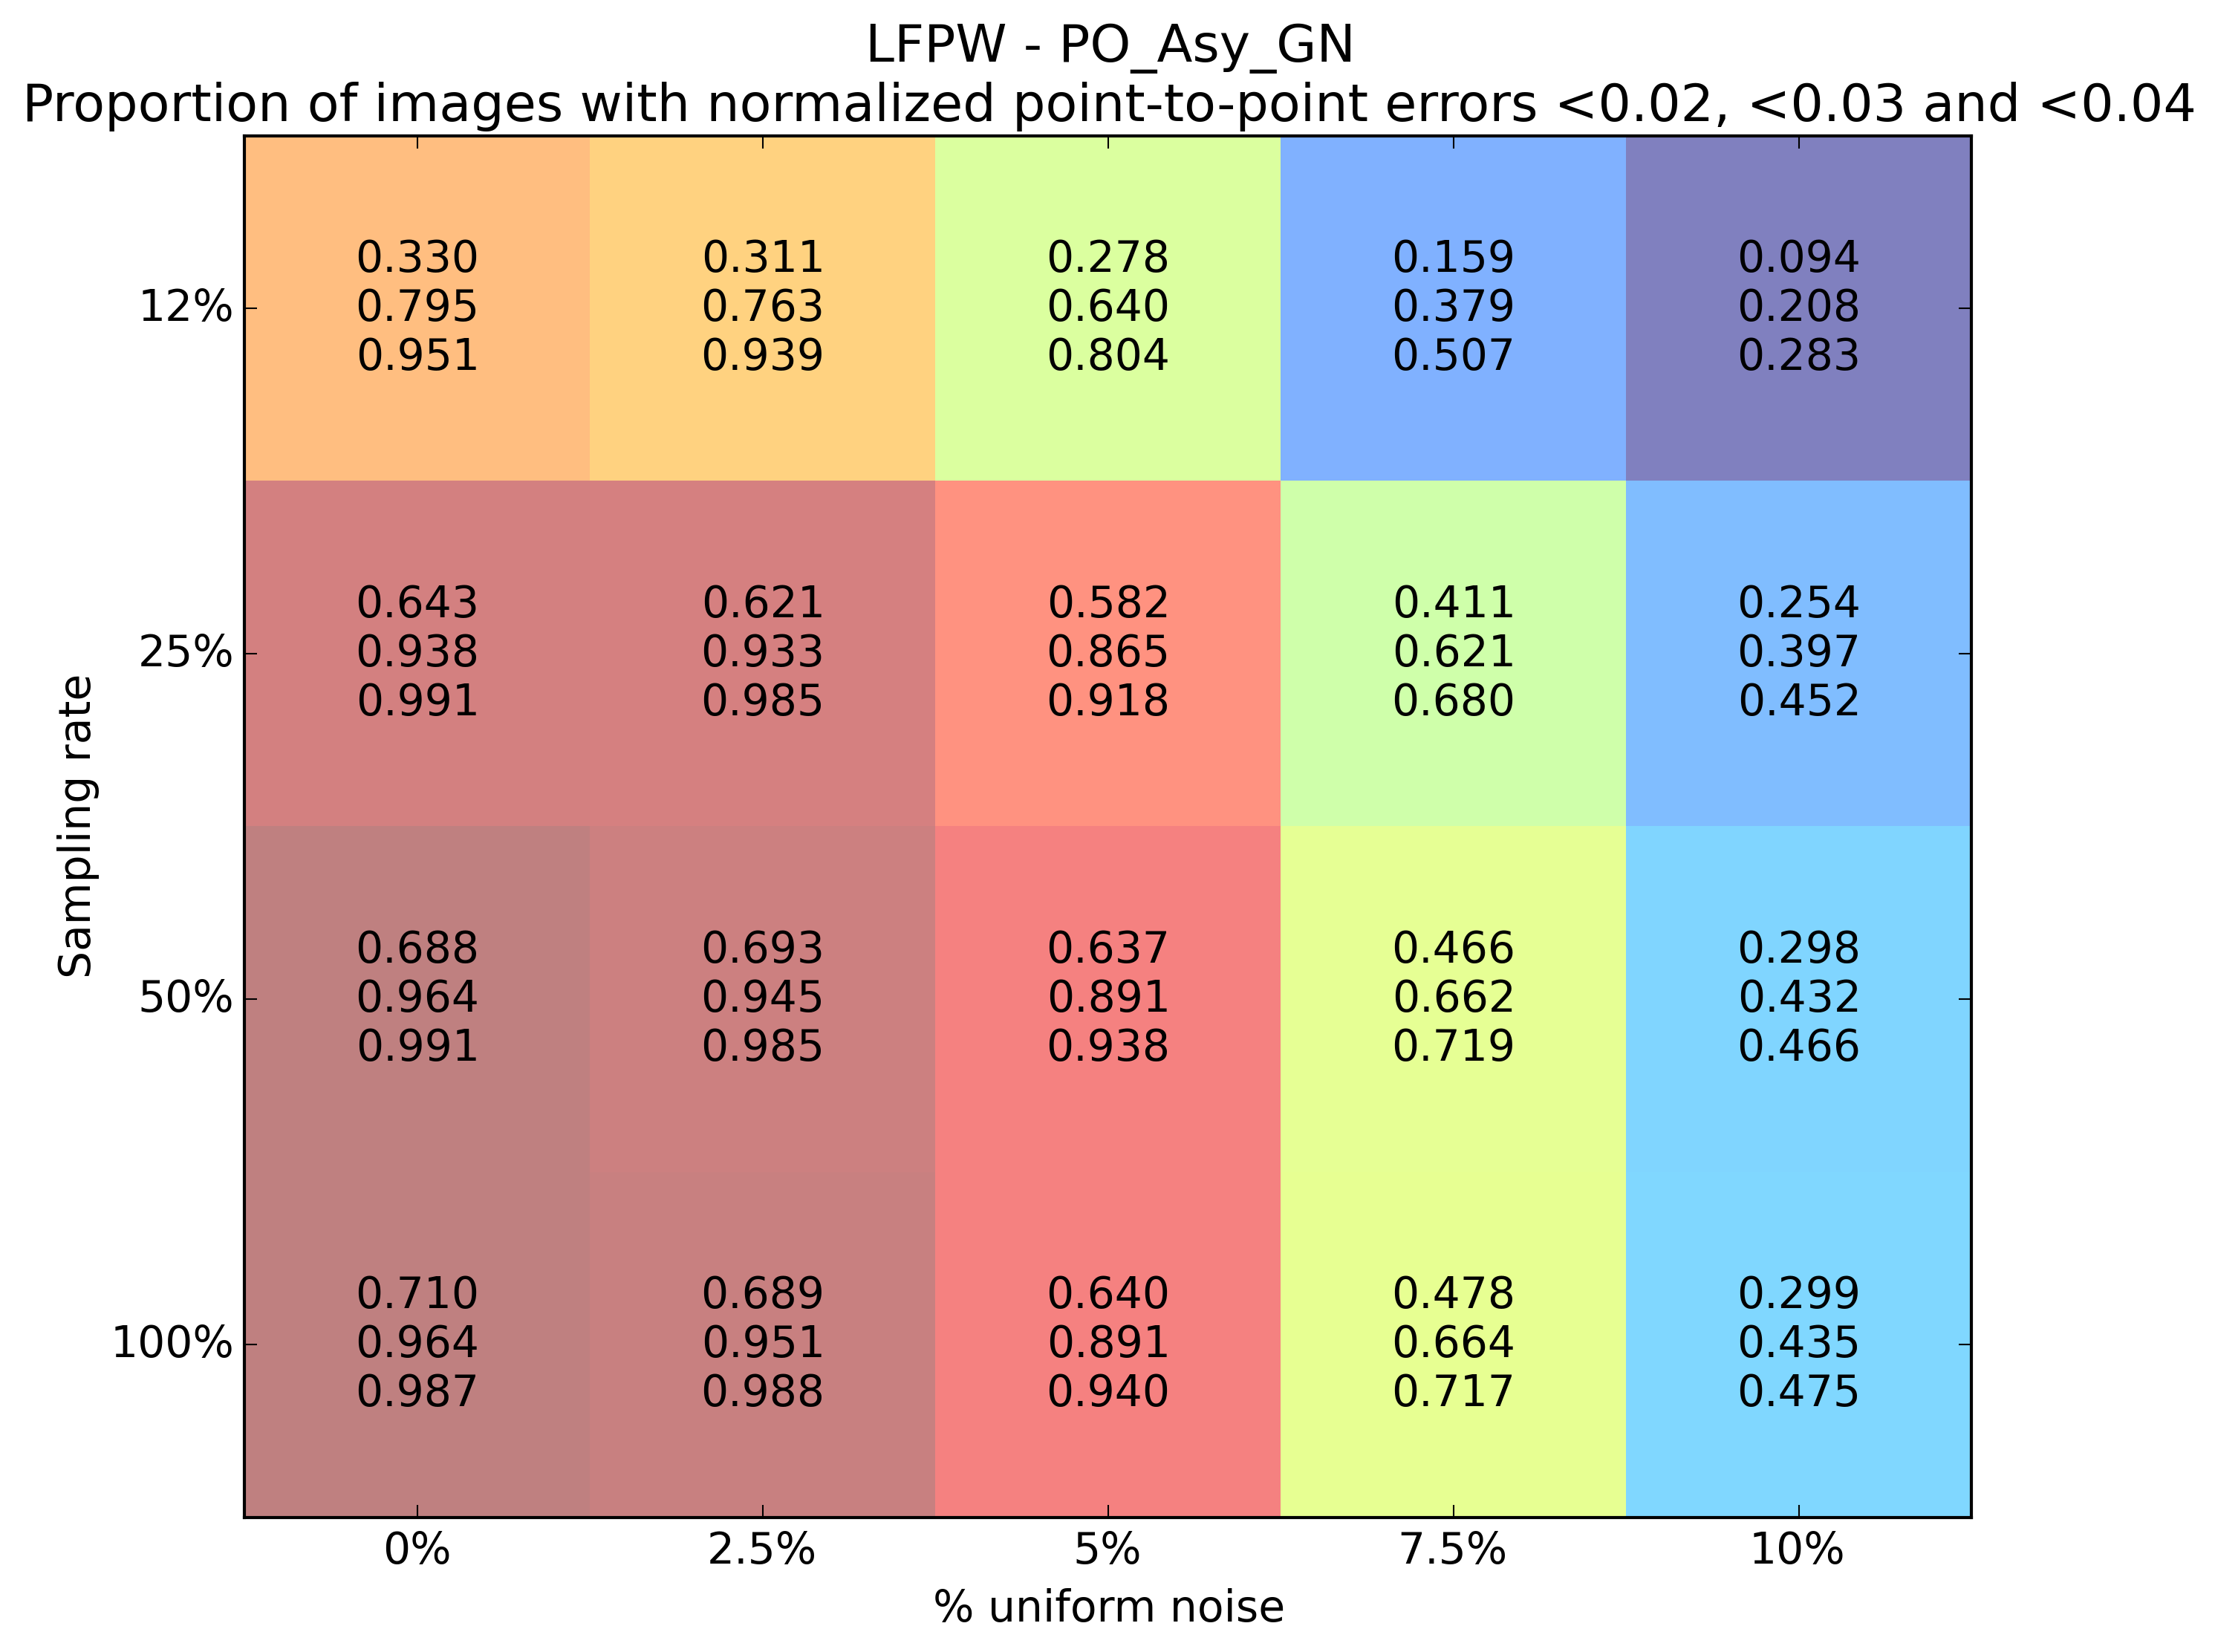
\includegraphics[width=\textwidth]{experiments/sampling/sampling_vs_noise_po_asy_gn.png}
	    \caption{Proportion of images with normalized point-to-point errors smaller than $0.02$, $0.03$ and $0.04$ for the Project-Out Asymmetric Gauss-Newton algorithm using different sampling rates, $40 (24 + 16)$ iterations, and initialized with different amounts of noise.}
	    \label{fig:sampling_vs_noise_po_asy_gn}
	\end{subfigure}
	\par\bigskip\bigskip
	\begin{subfigure}{\textwidth}
		\center
		\begin{tabular}{lcccccc}
		    \toprule
		    & $100\%$ & $<50\%$ & $<25\%$ & $<12\%$ 
		    \\
		    \midrule
		    PO\_Asy\_GN & $\sim1400$ ms & $\sim680$ ms & $\sim480$ ms & $\sim380$ ms
		    \\ 
		    PO\_Asy\_GN\_Sch & $\sim1680$ ms & $\sim930$ ms & $\sim650$ ms & $\sim590$ ms
		    \\
		    \bottomrule
	  	\end{tabular}
	  	\caption{Table showing run time of each algorithm for different amounts of sampling and $40 (24 + 16)$ iterations.}
	    \label{tab:runtime_40}
	\end{subfigure}
	\par\bigskip\bigskip
	\begin{subfigure}{0.48\textwidth}
	    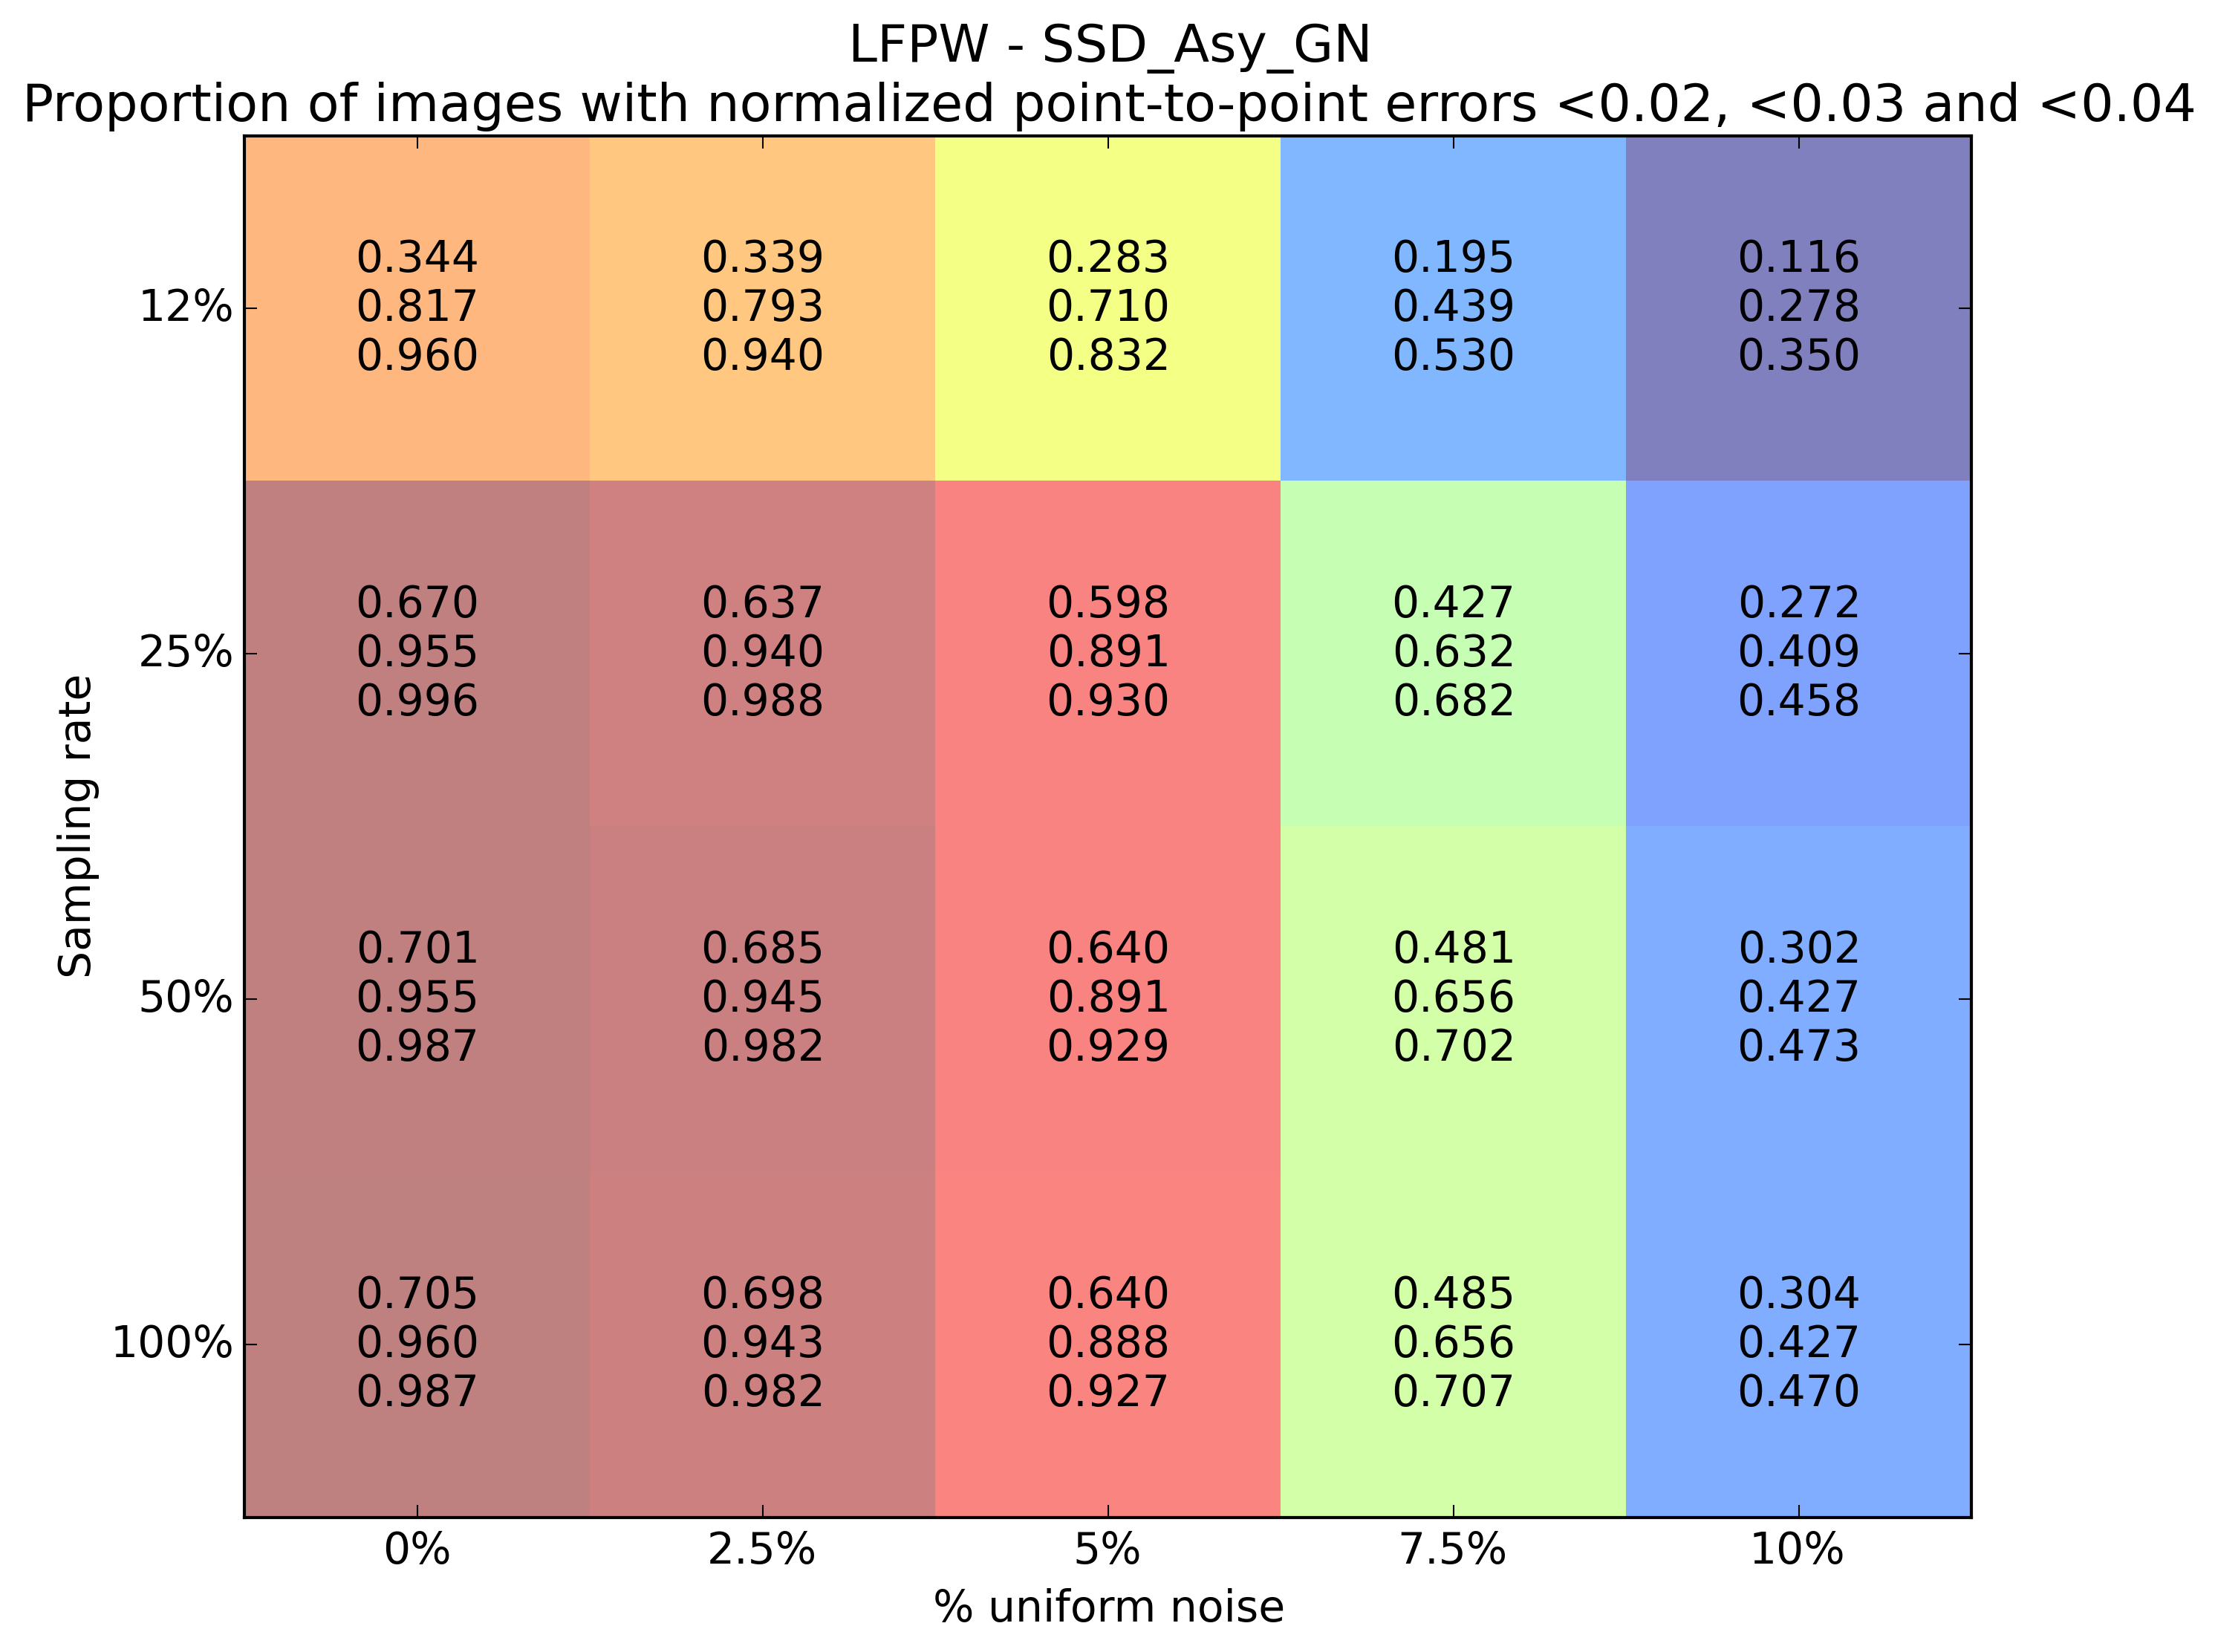
\includegraphics[width=\textwidth]{experiments/sampling/sampling_vs_noise_ssd_asy_gn.png}
	    \caption{Proportion of images with normalized point-to-point errors smaller than $0.02$, $0.03$ and $0.04$ for the SSD Asymmetric Gauss-Newton algorithm using different sampling rates, $20 (12 + 8)$ iterations, and initialized with different amounts of noise.}
	    \label{fig:sampling_vs_noise_ssd_asy_gn_20}
	\end{subfigure}
	\hfill
	\begin{subfigure}{0.48\textwidth}
	    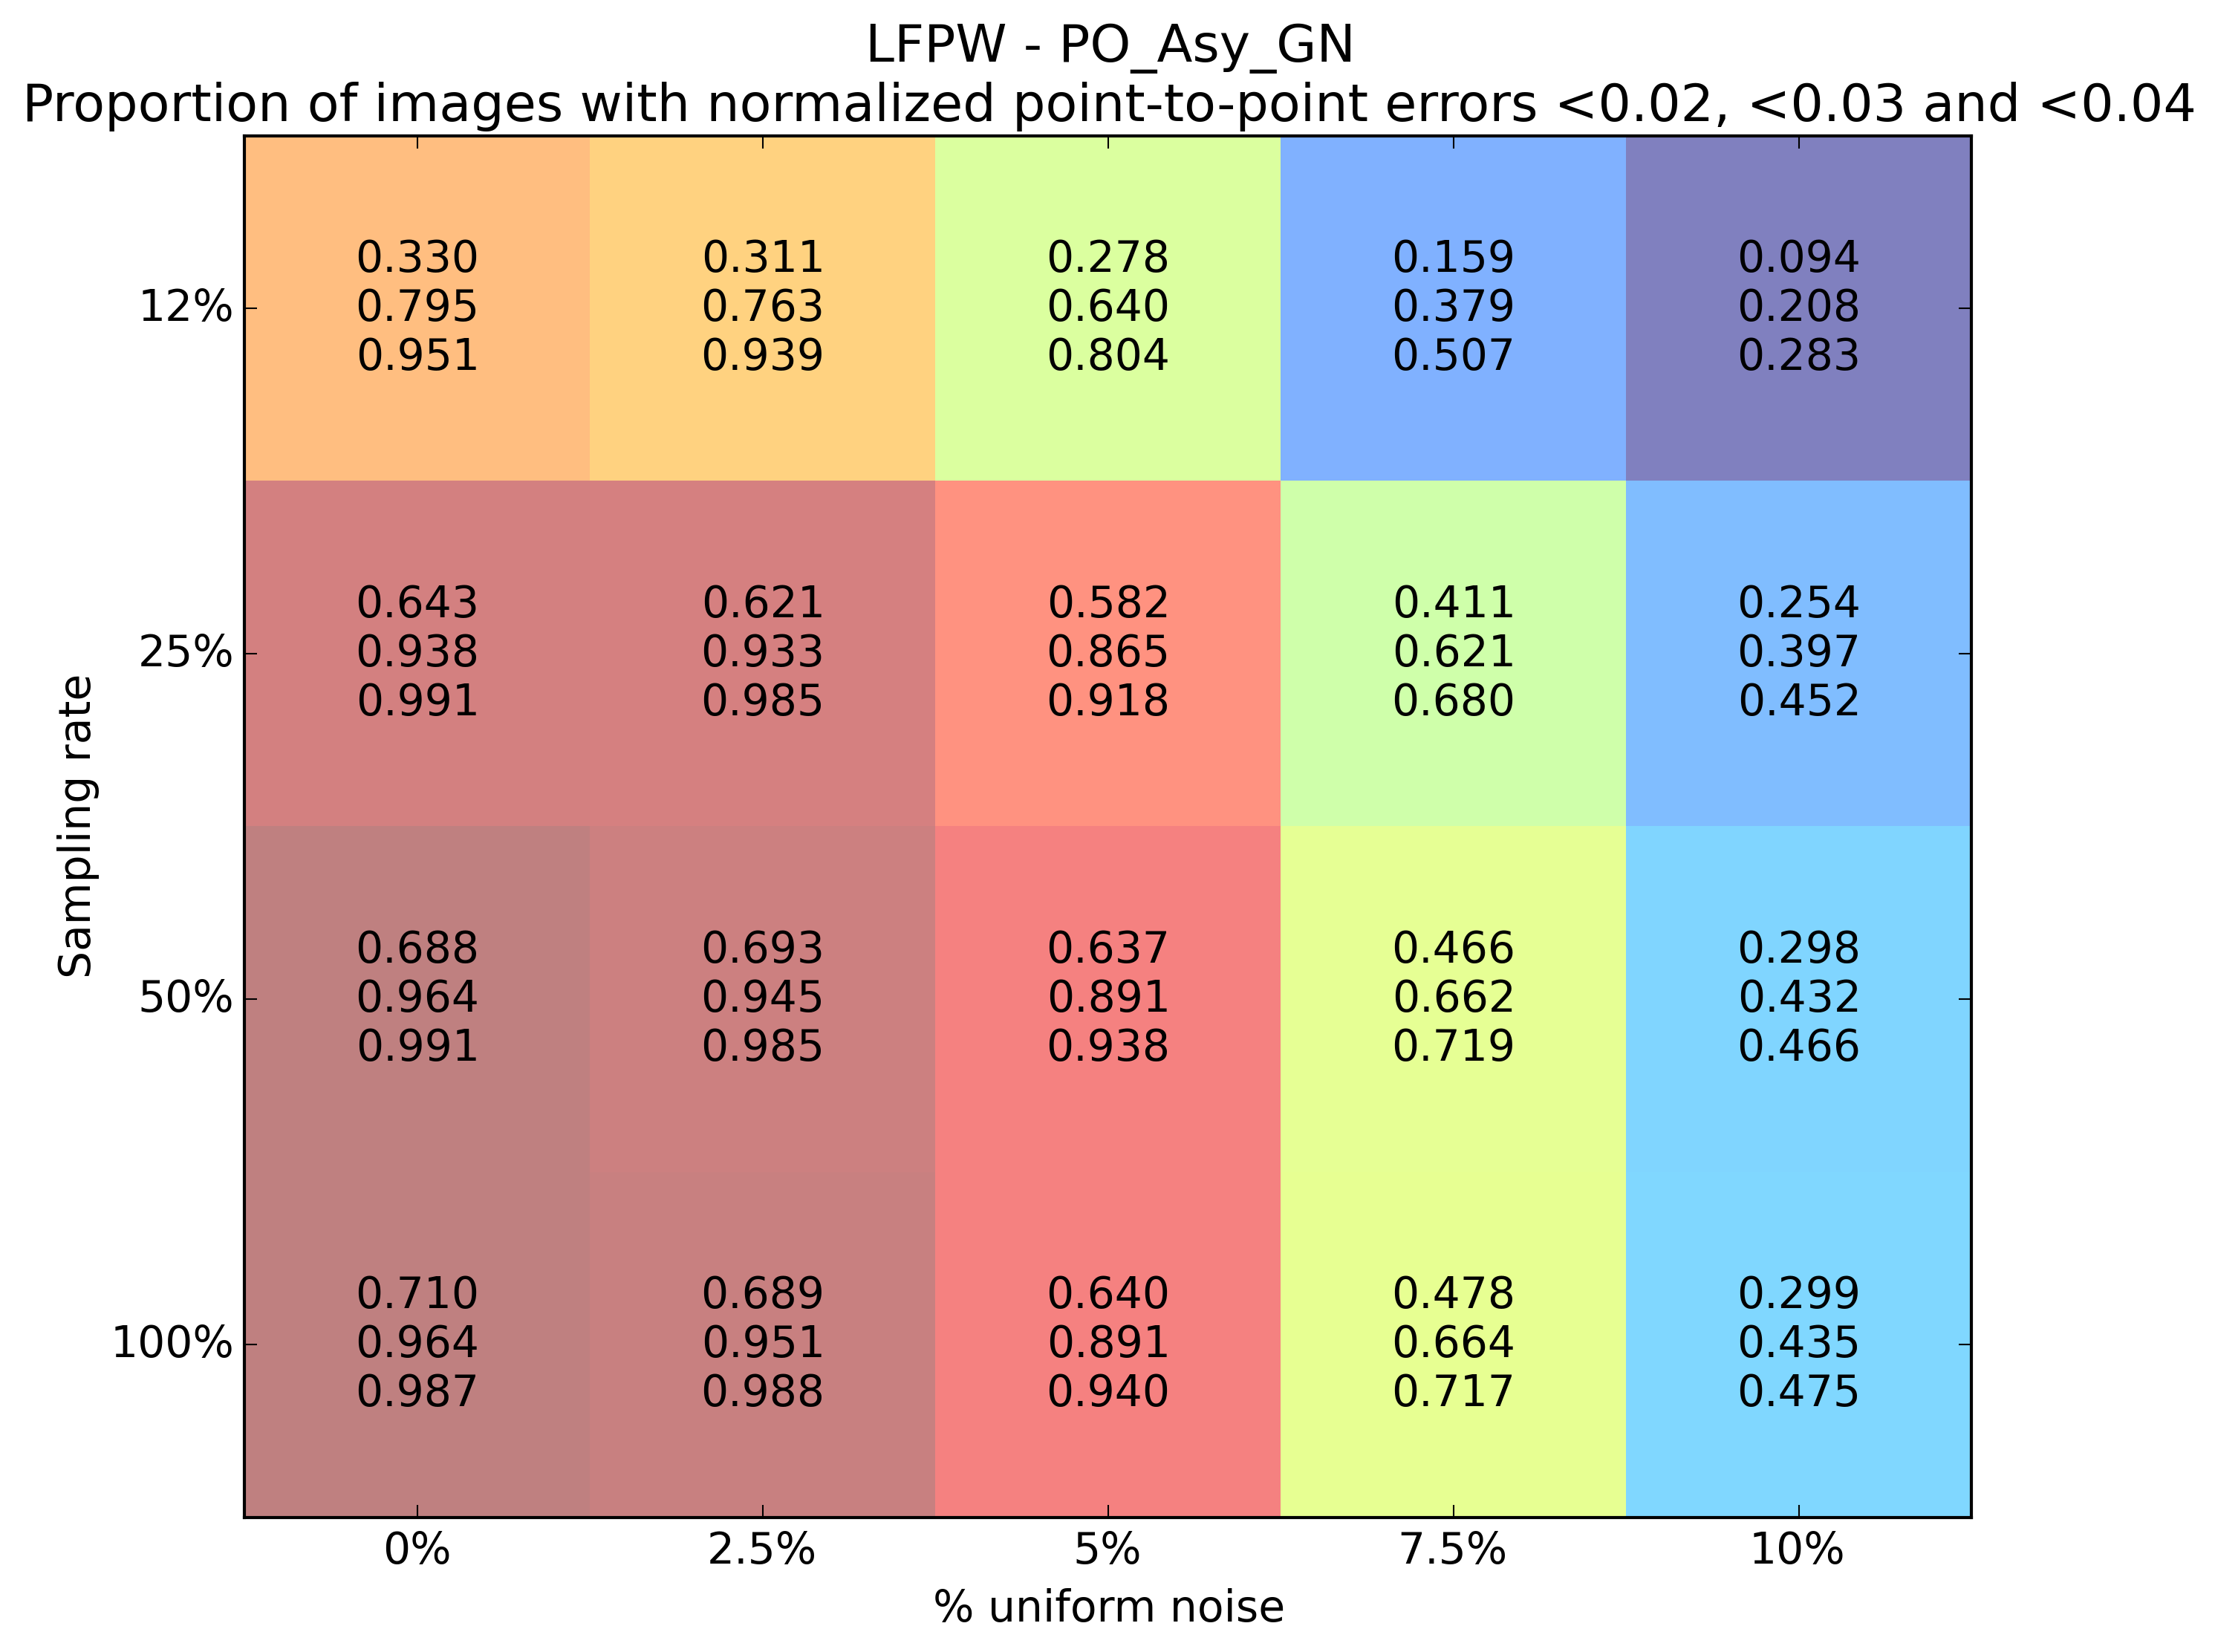
\includegraphics[width=\textwidth]{experiments/sampling/sampling_vs_noise_po_asy_gn.png}
	    \caption{Proportion of images with normalized point-to-point errors smaller than $0.02$, $0.03$ and $0.04$ for the Project-Out Asymmetric Gauss-Newton algorithm using different sampling rates, $20 (12 + 8)$ iterations, and initialized with different amounts of noise.}
	    \label{fig:sampling_vs_noise_po_asy_gn_20}
	\end{subfigure}
	\par\bigskip\bigskip
	\begin{subfigure}{\textwidth}
		\center
		\begin{tabular}{lcccccc}
		    \toprule
		    & $100\%$ & $<50\%$ & $<25\%$ & $<12\%$ 
		    \\
		    \midrule
		    PO\_Asy\_GN & $\sim1400$ ms & $\sim680$ ms & $\sim480$ ms & $\sim380$ ms
		    \\ 
		    PO\_Asy\_GN\_Sch & $\sim1680$ ms & $\sim930$ ms & $\sim650$ ms & $\sim596$ ms
		    \\
		    \bottomrule
	  	\end{tabular}
	  	\caption{Table showing run time of each algorithm for different amounts of sampling and $20 (12 + 8)$ iterations.}
	    \label{tab:runtime_20}
	\end{subfigure}
	\caption{Results assessing the effectiveness of sampling for the best performing Project-Out and SSD algorithms on the LFPW database.}
	\label{fig:sampling}
\end{figure*}


\subsection{Comparison on Helen and AFW}

In this last experiment, we report the fitting accuracy of the SSD and Project-Out Asymmetric Gauss-Newton algorithms on the test set of the Helen database and on the entire AFW database. We chose these two algorithm because they were the best performing algorithms in the previous experiments. 

\begin{figure*}[h!]
	\centering
	\begin{subfigure}{0.48\textwidth}
	    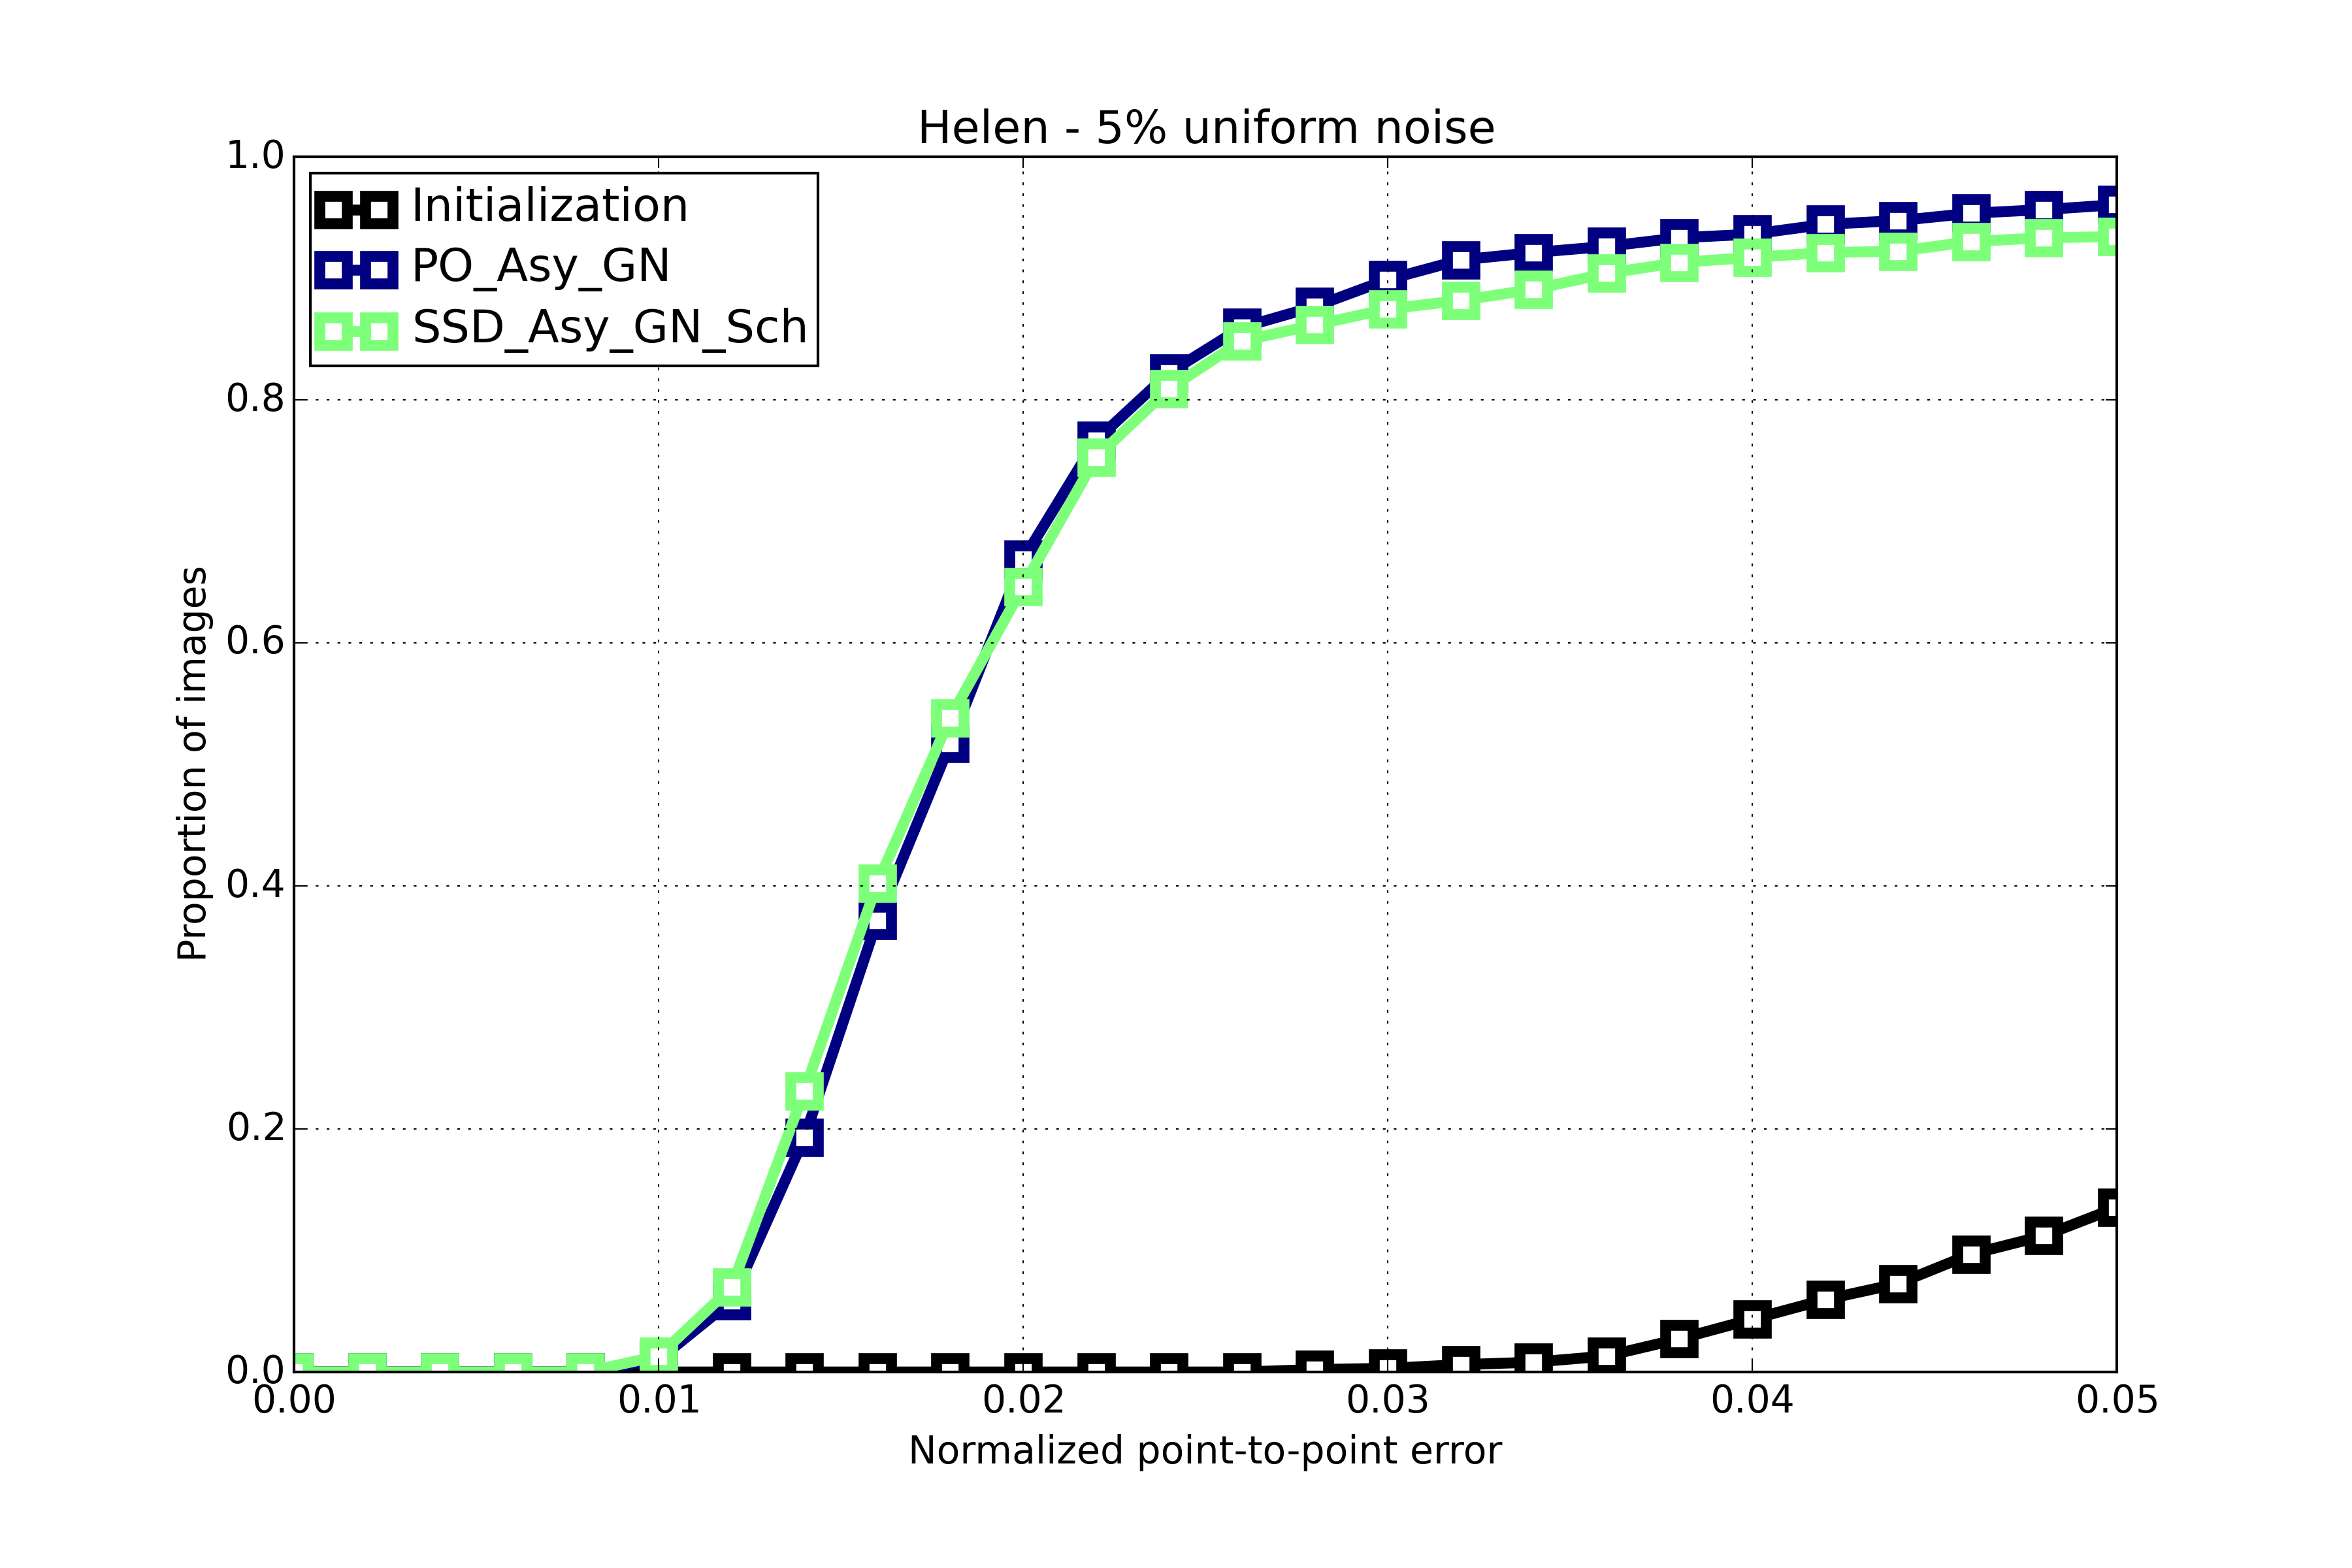
\includegraphics[width=\textwidth]{experiments/best/ced_helen_5.png}
	    \caption{CED on the Helen test dataset for the Project-Out and SSD Asymmetric Gauss-Newton algorithms initialized with $5\%$ noise.}
	    \label{fig:ced_po_for_gn}
	\end{subfigure}
	\hfill
	\begin{subfigure}{0.48\textwidth}
	    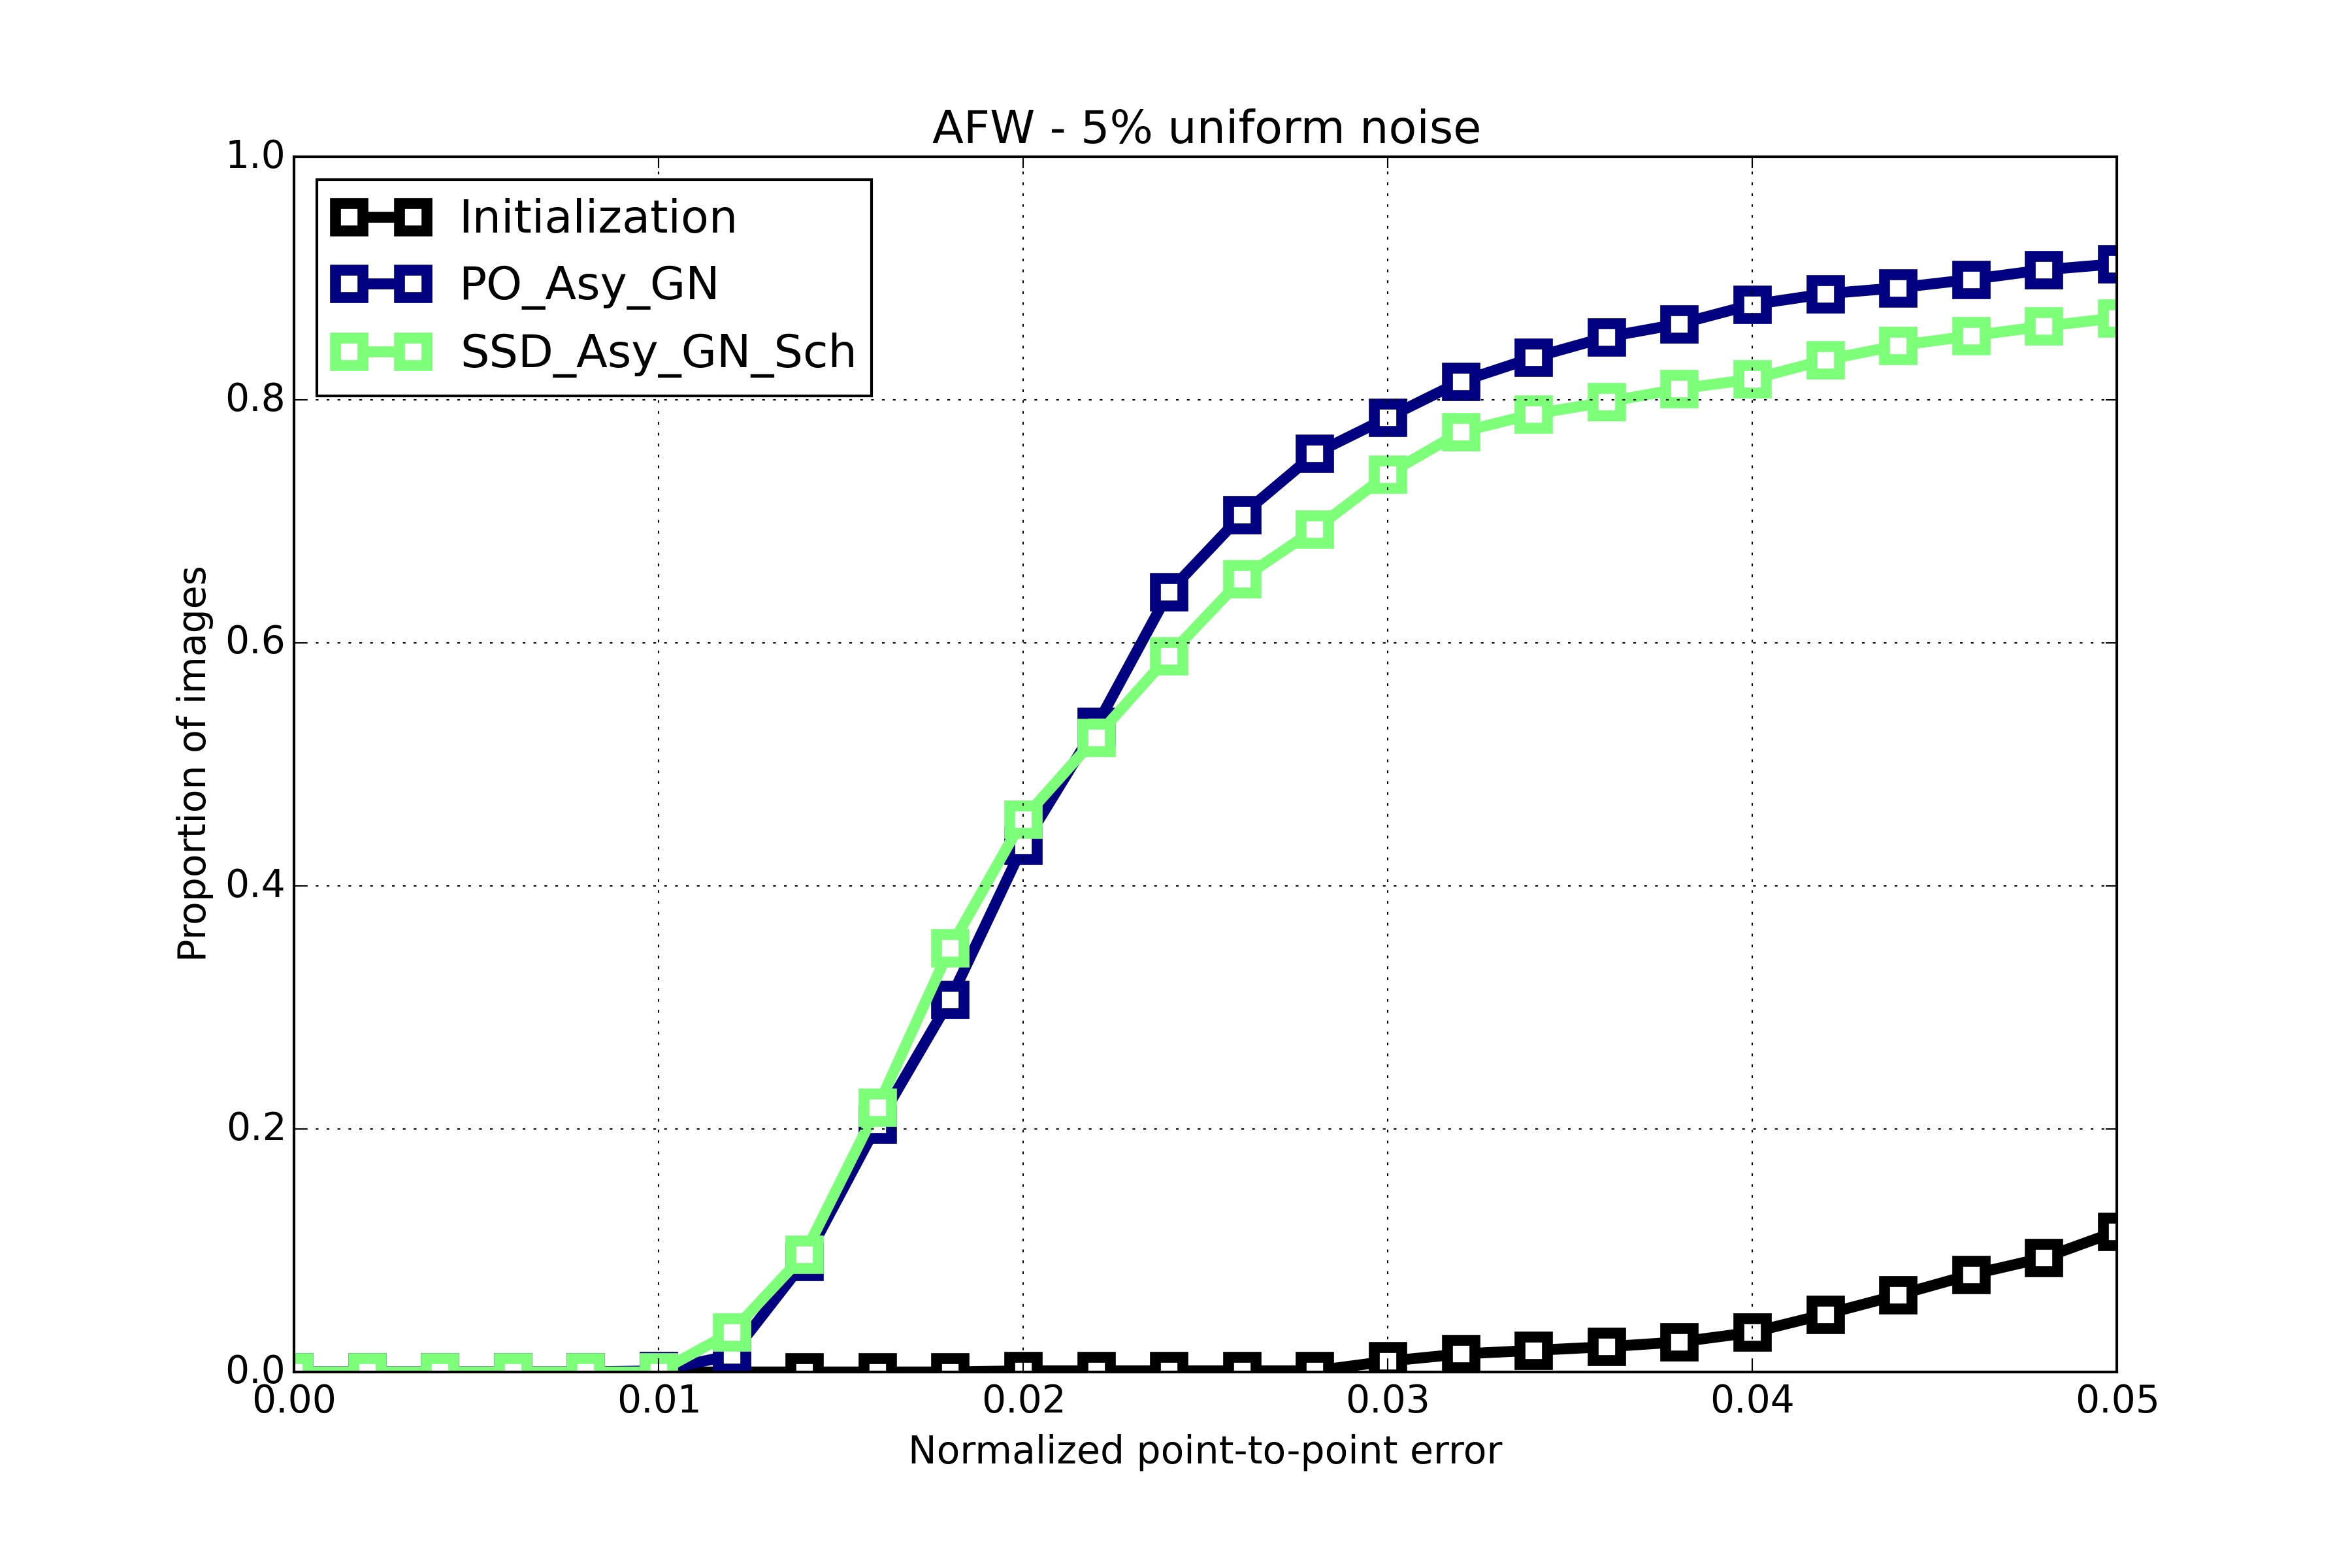
\includegraphics[width=\textwidth]{experiments/best/ced_afw_5.png}
	    \caption{CED on the AFW database for the Project-Out and SSD Asymmetric Gauss-Newton algorithm initialized with $5\%$ noise.}
	    \label{fig:ced_po_inv_gn}
	\end{subfigure}
	\caption{Results showing the fitting accuracy of the SSD and Project-Out Asymmetric Gauss-Newton algorithms on the Helen and AFW databases.}
	\label{fig:helen_afw}
\end{figure*}

% \begin{figure*}[h!]
% 	\centering
% 	\begin{subfigure}{0.48\textwidth}
% 	    \includegraphics[width=\textwidth]{experiments/best/helen/ced_best_5.png}
% 	    \caption{Cumulative Error Distribution on the entire AFW database for the best performing CGD algorithms initialized with $5\%$ uniform noise.}
% 	    \label{fig:helen_ced_best_5}
% 	\end{subfigure}
% 	\hfill
% 	\begin{subfigure}{0.48\textwidth}
% 		\includegraphics[width=\textwidth]{experiments/best/afw/ced_best_5.png}
% 	    \caption{Cumulative Error Distribution on the AFW database for the best performing CGD algorithms initialized with $5\%$ uniform noise.}
% 	    \label{fig:afw_ced_best_5}
% 	\end{subfigure}
% 	\label{fig:helen_afw}
% 	\caption{Experimental results on the Helen and AFW databases.}
% \end{figure*}


% \begin{figure*}[h!]
% 	\centering
% 	\begin{subfigure}{0.48\textwidth}
% 	    \includegraphics[width=\textwidth]{experiments/best/helen/ced_best_5.png}
% 	    \caption{Cumulative Error Distribution on the entire AFW database for the best performing CGD algorithms initialized with $5\%$ uniform noise.}
% 	    \label{fig:helen_ced_best_5}
% 	\end{subfigure}
% 	\hfill
% 	\begin{subfigure}{0.48\textwidth}
% 	    \includegraphics[width=\textwidth]{experiments/best/helen/mean_error_vs_iters_best_5.png}
% 	    \caption{Mean normalized point-to-point error vs number of iterations on the entire AFW database for the best performing CGD algorithms initialized with $5\%$ uniform noise.}
% 	    \label{fig:helen_mean_error_vs_iters_best_5}
% 	\end{subfigure}
% 	\par\bigskip
% 	\begin{subfigure}{0.48\textwidth}
% 	    \includegraphics[width=\textwidth]{experiments/best/helen/mean_cost_vs_iters1_best_5.png}
% 	    \caption{Mean normalized cost vs number of first pyramid level iterations on the entire AFW database for the best performing CGD algorithms initialized with $5\%$ uniform noise.}
% 	    \label{fig:helen_mean_cost_vs_iters1_best_5}
% 	\end{subfigure}
% 	\hfill
% 	\begin{subfigure}{0.48\textwidth}
% 	    \includegraphics[width=\textwidth]{experiments/best/helen/mean_cost_vs_iters2_best_5.png}
% 	    \caption{Mean normalized cost vs number of first pyramid level iterations on the entire AFW database for the best performing CGD algorithms initialized with $5\%$ uniform noise..}
% 	    \label{fig:helen_mean_cost_vs_iters2_best_5}
% 	\end{subfigure}
% 	\label{fig:helen}
% 	\caption{Experimental results on the Helen database.}
% \end{figure*}


% \begin{figure*}[h!]
% 	\centering
% 	\begin{subfigure}{0.48\textwidth}
% 	    \includegraphics[width=\textwidth]{experiments/best/afw/ced_best_5.png}
% 	    \caption{Cumulative Error Distribution on the AFW database for the best performing CGD algorithms initialized with $5\%$ uniform noise.}
% 	    \label{fig:afw_ced_best_5}
% 	\end{subfigure}
% 	\hfill
% 	\begin{subfigure}{0.48\textwidth}
% 	    \includegraphics[width=\textwidth]{experiments/best/afw/mean_error_vs_iters_best_5.png}
% 	    \caption{Mean normalized point-to-point error vs number of iterations on the AFW database for the best performing CGD algorithms initialized with $5\%$ uniform noise.}
% 	    \label{fig:afw_mean_error_vs_iters_best_5}
% 	\end{subfigure}
% 	\par\bigskip
% 	\begin{subfigure}{0.48\textwidth}
% 	    \includegraphics[width=\textwidth]{experiments/best/afw/mean_cost_vs_iters1_best_5.png}
% 	    \caption{Mean normalized cost vs number of first pyramid level iterations on the AFW database for the best performing CGD algorithms initialized with $5\%$ uniform noise.}
% 	    \label{fig:afw_mean_cost_vs_iters1_best_5}
% 	\end{subfigure}
% 	\hfill
% 	\begin{subfigure}{0.48\textwidth}
% 	    \includegraphics[width=\textwidth]{experiments/best/afw/mean_cost_vs_iters2_best_5.png}
% 	    \caption{Mean normalized cost vs number of first pyramid level iterations on the AFW database for the best performing CGD algorithms initialized with $5\%$ uniform noise..}
% 	    \label{fig:afw_mean_cost_vs_iters2_best_5}
% 	\end{subfigure}
% 	\label{fig:afw}
% 	\caption{Experimental results on the AFW database.}
% \end{figure*}



% This section reports the performance of the proposed method on the problem of face alignment in-the-wild. Results for two different experiments are reported. The first experiment compares the accuracy and convergence properties of the proposed Unified PIC-RLMS and AIC-RLMS algorithms with respect to those of PIC \cite{Baker2004}, AIC \cite{Papandreou2008} and and RLMS \cite{Saragih2011} on the popular LFPW \cite{Belhumeur2011} and Helen \cite{Le2012} datasets. The second experiment compares the performance of the previous algorithms against recently proposed state-of-the-art methods for face alignment in-the-wild, \ie the Supervised Descent Method of Xiong and De La Torre \cite{Xiong2013} and the Gauss-Newton Deformable Parts Model of Tzimiropoulos and Pantic \cite{Tzimiropoulos2014}, on the very challenging Annotated Faces in the Wild (AFW) dataset.

% \subsection{Comparison with AAMs and CLMs}
% Results for this experiment are reported over the 224 and 330 test images of the LFPW \cite{Belhumeur2011} and Helen\cite{Le2012} datasets. 66 points ground truth landmark annotations were provided by the iBUG group\footnote{\label{ibug_300}\url{http://ibug.doc.ic.ac.uk/resources/300-W/}}. All methods were initialized by perturbing the ground truth scale and translation parameters with Gaussian noise (rotations were not considered) and applying the resulting transformation to mean of the shape model. (Notice that this procedure produces initializations that are considerably more challenging than those reported in the recent AAM literature \cite{Tzimiropoulos2013, Tzimiropoulos2014}). The Cumulative Error Distributions (CED) for this experiment is shown in Figures \ref{fig:lfpw_exp1} and \ref{fig:helen_exp1}. Figures \ref{fig:lfpw_exp2} and \ref{fig:helen_exp2} shows the evolution of the mean normalized point-to-point error as a function of the number of iterations run by each algorithm. This experiment shows that our Unified AIC-RLMS approach considerably outperforms all other methods by a large margin on both datasets. More specifically, AIC-RLMS achieves a constant improvement of between 10\% to 20\% over PIC-RLMS and AIC at the significant region $0.020 < err > 0.040$ (at which the results are generally considered adequate by visual inspection). Note that the fast Unified PIC-RLMS algorithm is also the second most performant algorithm, surpassing both AIC and RLMS, on this particular experiment.

% \subsection{Comparison with state of the art}

% Results for this experiment are reported over the 337 images of the AFW \cite{Zhu2012} dataset. In this case, 49 points ground truth landmark annotations for this dataset were again provided by the iBUG group\footnoteref{ibug_300}. Results for \cite{Xiong2013} and \cite{Tzimiropoulos2014} were directly obtained using the publicly available models and fitting code kindly provided by the authors\footnote{\url{http://www.humansensing.cs.cmu.edu/intraface/}}$^{,}$\footnote{\url{http://ibug.doc.ic.ac.uk/resources/gauss-newton-deformable-part-models-face-alignment/}}. Note that, the provided models have been potentially trained using thousands of images in contrast to the only 813 images used to trained our method. In this experiment, all algorithms were initialized using the bounding box provided by our own in-house implementation of the face detector of \cite{Zhu2012}. The CED for this experiment are reported in Figure \ref{fig:afw_exp}. The results show that our Unified AIC-RLMS algorithm achieves state-of-the-art results on the AFW dataset, considerably outperforming both the Gauss-Newton Deformable Parts-Model of Tzimiropoulos and Pantic \cite{Tzimiropoulos2014} (which can be extremely accurate but sensitive to inaccurate initializations) and the SDM method of Xiong and De la Torre \cite{Xiong2013} (which can deal with very noisy initializations but is significantly less accurate than our method).

% \begin{figure}[t!]
% \centering
% \includegraphics[width=0.38\textwidth]{figures/graph7.png}
% \caption{Cumulative Error Distributions over 49 landmarks for the AFW dataset.}
% \label{fig:afw_exp}
% \end{figure}
